\documentclass[a4paper,10pt]{article}
\usepackage[top=25mm,bottom=24mm,left=27mm,right=27mm,headheight=15pt,headsep=8mm,footskip=12mm]{geometry}
\usepackage{fontspec,amsmath,amsthm,unicode-math}
\usepackage[english]{babel}
\usepackage{microtype,xcolor,fancyhdr,titlesec,booktabs,longtable,array,tabularx}
\usepackage{graphicx,tikz,enumitem,float,needspace}
\usetikzlibrary{arrows.meta,calc,positioning,decorations.pathreplacing,matrix}
\usepackage[unicode,hidelinks]{hyperref}
\usepackage[nameinlink,noabbrev]{cleveref}
\setmainfont{STIXTwoText-Regular.otf}[BoldFont=STIXTwoText-Bold.otf,ItalicFont=STIXTwoText-Italic.otf,BoldItalicFont=STIXTwoText-BoldItalic.otf]
\setmathfont{STIXTwoMath-Regular.otf}
\hypersetup{pdftitle={Coinductive generation of π, φ and e to arbitrary depth, derivation of α and the algebraic structure of the electron},pdfauthor={Oumar Haidara Fall; Rubén Ramos Balsa},pdfsubject={Compilation manuscript for academic transfer}}
\newcommand{\Autores}{Oumar Haidara Fall \textperiodcentered\ Rubén Ramos Balsa}
\newcommand{\Titulo}{Coinductive generation of \(\pi\), \(\varphi\) and \(e\) to arbitrary depth, derivation of \(\alpha\) and the algebraic structure of the electron}
\newcommand{\RR}{\mathbb R}\newcommand{\ZZ}{\mathbb Z}\newcommand{\QQ}{\mathbb Q}\newcommand{\CC}{\mathbb C}\newcommand{\FF}{\mathbb F}
\newcommand{\Id}{\operatorname{id}}\newcommand{\tr}{\operatorname{tr}}
\newcommand{\Span}{\operatorname{span}}\newcommand{\Cyl}{\operatorname{Cyl}}
\newcommand{\square}{\mdlgwhtsquare}
\newcommand{\TPK}{\mathrm{TPK}}\newcommand{\APP}{\mathrm{APP}}\newcommand{\TRIT}{\{-1,0,+1\}}
\newtheorem{theorem}{Theorem}[section]
\newtheorem{lemma}[theorem]{Lemma}
\newtheorem{proposition}[theorem]{Proposition}
\newtheorem{corollary}[theorem]{Corollary}
\theoremstyle{definition}
\newtheorem{definition}[theorem]{Definition}
\newtheorem{axiom}[theorem]{Axiom}
\theoremstyle{remark}\newtheorem{remark}[theorem]{Remark}
\numberwithin{equation}{section}
\setlength{\parindent}{1em}\setlength{\parskip}{3pt plus 1pt minus .5pt}
\setlength{\emergencystretch}{2em}
\clubpenalties 3 10000 10000 0
\widowpenalties 3 10000 10000 0
\displaywidowpenalty=10000
\renewcommand{\normalsize}{\fontsize{10.5}{13.4}\selectfont}\normalsize
\setlist{nosep,topsep=5pt}
\titleformat{\section}{\fontsize{13}{16}\selectfont\bfseries}{\thesection}{.65em}{}
\titleformat{\subsection}{\fontsize{11.2}{14}\selectfont\bfseries}{\thesubsection}{.65em}{}
\titleformat{\subsubsection}{\normalsize\bfseries}{\thesubsubsection}{.65em}{}
\AddToHook{cmd/subsection/before}{\Needspace{7\baselineskip}}
\AddToHook{cmd/subsubsection/before}{\Needspace{6\baselineskip}}
\AddToHook{env/theorem/before}{\Needspace{7\baselineskip}}
\AddToHook{env/lemma/before}{\Needspace{7\baselineskip}}
\AddToHook{env/proposition/before}{\Needspace{7\baselineskip}}
\setcounter{tocdepth}{2}
% REV03: preserve a separate number box for two-digit subsections.
\makeatletter
\renewcommand{\l@subsection}{\@dottedtocline{2}{1.5em}{3.2em}}
\makeatother
\titlespacing*{\section}{0pt}{17pt}{9pt}\titlespacing*{\subsection}{0pt}{13pt}{6pt}
\pagestyle{fancy}\fancyhf{}
\fancyhead[L]{\fontsize{8}{10}\selectfont Coinductive generation and algebraic structure of the electron}
\fancyhead[R]{}
\fancyfoot[C]{\thepage}\renewcommand{\headrulewidth}{.2pt}
\raggedbottom
% BEGIN NUCLEO_ADITIVO_20260921_PREAMBULO
\makeatletter
\@ifundefined{example}{\theoremstyle{definition}\newtheorem{example}[theorem]{Example}}{}
\@ifundefined{notatabla}{\newcommand{\notatabla}[1]{\par\smallskip{\footnotesize #1\par}}}{}
\makeatother
\providecommand{\FF}{\mathbb F}

% END NUCLEO_ADITIVO_20260921_PREAMBULO
% Apertura independiente del índice: corrección quirúrgica 20260928.
\let\HMTIndiceOriginal\tableofcontents
\makeatletter
\renewcommand{\tableofcontents}{\clearpage\begingroup\setlength{\parskip}{0pt}\fontsize{9.2}{10.5}\selectfont
\renewcommand{\l@section}[2]{\addvspace{3pt}\begingroup\bfseries\@dottedtocline{1}{0pt}{2em}{##1}{##2}\endgroup}
\HMTIndiceOriginal\endgroup\clearpage}
\makeatother
\begin{document}
\thispagestyle{plain}
\begin{center}
{\fontsize{9.5}{10.7}\selectfont Compilation manuscript for academic transfer\par}
\vspace{6mm}
{\fontsize{17}{20.5}\selectfont\bfseries\Titulo\par}
\vspace{8pt}
{\fontsize{11.5}{14}\selectfont\Autores\par}
\vspace{4pt}
{\fontsize{8}{10}\selectfont Coauthorship without precedence of contribution\par}
\vspace{4pt}
{\fontsize{8}{10}\selectfont Documentary integration and compilation generated by ChatGPT - Astra.\par}
\end{center}
\vspace{3pt}
\begin{center}\bfseries Abstract\end{center}
\begingroup
\fontsize{9.5}{10.7}\selectfont
\setlength{\parskip}{1.5pt plus .5pt minus .5pt}
\noindent
The constants \(\pi,\varphi,e\) are generated coinductively and jointly to arbitrary depth,
the fine-structure constant \(\alpha\) is derived, and the electronic
coordinate, its spin-\(1/2\) representation, and its helicity components
are constructed. The construction relates the determination of these
values to the preservation of the structures that produce them.
Its foundation is \emph{Triadic Modular Holography} (HMT):
\emph{All Possible Paths} (APP) is the discrete toroidal support
\((\mathbb Z/9\mathbb Z)^2\), equipped with the additive Cayley graph
generated by \(\pm(1,0),\pm(0,1)\) and with addition and multiplication
evaluations; TRIT is the oriented ternary signature \(\{-1,0,+1\}\),
which distinguishes three quadratic regimes; the \emph{Topological Phase
Kernel} (TPK) composes phase selection, transport, and memory updating.

The 104\,976 oriented initial conditions produce 468 emissions and 243
visible ternary sequences. Regions of closure, propagation, and self-scaling
are determined in this domain, whose Archimedean realizations are
\(\pi,e,\varphi\). Refinement by compatible cylinders makes it possible to obtain
any finite prefix by a finite computation. Nonadic holonomy preserves
phase while increasing memory; its aperiodic representation makes explicit
the coexistence of modular periodicity and unlimited prolongation.

The integral dodecaphase record \(K\) and its periodic rational realization
\(\kappa\) admit reversible reconstructions. Their composition with the regional
records determines \(\alpha\) by positional normalization. The correlated
analytic route represents it as the unique simple root of a prolongation
of the vacancy resolvent, with an explicit recurrence and geometric class.
Compatibility at every depth proves equality of the two representations
of the same state. Scalar evaluation and incidence resolution
are articulated through the oriented records that both preserve.

The electronic construction brings together the center of APP, oriented vacancy,
a matrix representation of the three regimes, and transfer between
areal and volumetric evaluations. The spin-\(1/2\) generators and directional
projectors are constructed from the electronic block; their interpretation
as helicity declares the direction of propagation and preserves scalar
evaluation, charge orientation, and route memory as distinct data.
Two readers of the return determine
the coefficients of its complete composition. The central trajectory visits
exactly \(27\) cells; its oriented event histories are distinguished by
the reversible integral chart. The harmonic decomposition of the return
has modes \(2,6,10\), whose powers \(64,16,64\) recover the coefficients
\(80\) and \(6\) of the electronic correction.
The action scale and
dimensional realization are presented before comparison with CODATA 2018 and
2022. The second realization of the structure preserves boundary
incidence: Witt designs, Golay codes, the Leech lattice, and the vertex
algebra \(V^\natural\), with its automorphism group, the Monster.
The numerical and exceptional realizations arise from the same structure;
their local operations and compatible limits preserve the records
linking equations, values, and incidence.
The record \(K\) also selects the direction of the reduction
\(11\to10\). Orbifolds of orders \(2\) and \(3\) provide isomorphic
presentations of \(V^\natural\), with transport of their automorphisms
and graded traces. The isomorphism of the quotient screens intertwines
reciprocal-radius duality while preserving the reduction data of
\(K\) and the lattice screen.

% BEGIN S27_FRAMING
Comparison of the stars of \(B_K\), \(B_\varphi\), and
\(B_{\rm APP}\) distinguishes their twelve completions through a common
polarization and places their signatures within the classification of
the \(495\) four-subsets. The ordered frame
\((H^-_\alpha,H_e,H_\varphi,H_{\rm APP})\) has trivial stabilizer
in the constructed incidence group. The carry cocycle, in turn,
makes explicit the information in the integer quotients that complements
the residues of the regional columns. Its composition and transport laws
preserve the arithmetic lift associated with numerical reading, while
the stars and their stabilizers determine the organization of boundary
reading.

% END S27_FRAMING
\vspace{7pt}
Transport monodromy and the mathematical model of an aperiodic time
crystal connect modular return, memory advance, and the three regimes
of the exponential. The determinantal decade and action character
determine the section corresponding to the reduced Planck constant,
\(\hbar\), that enters the electronic composition.



% BEGIN R27_FRAMING_SUMMARY_EN
The precision of this chain is developed from the arithmetic of the
emitter: its decimal alphabet of \(42\) blocks is determined, junctions
between regional emissions are exhibited, and ordered memory is
distinguished from the marginal distribution. Boundary selection separates
saturation, dual neutrality, and orientation. APP refinement laws, the
index-two sublattice, nonadic addition with carry, and quadratic correlation
make the intermediate operations explicit. In the level-three realization,
a formal-series identity yields optimal uniform divisibility by \(3^9\).
% END R27_FRAMING_SUMMARY_EN

\noindent\textbf{Keywords:} structural derivation of fundamental constants;
Triadic Modular Holography; coinductive generation; fine-structure constant;
algebraic structure of the electron; holonomy; boundary incidence;
reduced Planck constant; monodromy; aperiodic time crystal;
exceptional symmetries; Moonshine.
\par\endgroup

\tableofcontents
\clearpage
\begingroup\setlength{\parskip}{2pt}\fontsize{10}{11.8}\selectfont
\section{Introduction}
\label{sec:introduccion}

This work establishes a common coinductive generation of
\(\pi,\varphi,e\), the dodecaphase closure of \(\alpha\) and its
correlated analytic representation, and the algebraic composition of
the electronic coordinate. The electronic block also determines a
spin-\(1/2\) representation whose projectors give helicities
\(\pm1/2\) when a direction of propagation is specified. The same
genealogy preserves an incidence record leading to the Witt designs,
Golay codes, the Leech lattice, and \(V^\natural\). The result thus
connects determined values, recoverable memory, and algebraic
realizations through explicit operations.

Determining the values of fundamental constants constitutes a
central question in mathematical physics. A theory may establish relations
among observables, identify symmetries, and organize highly precise predictions,
while retaining parameters whose values are determined experimentally.
Understanding why those parameters take their values requires a construction
that identifies the operations, normalizations, and compatibility
conditions from which they result. This is the question organizing the present
work: the relation between the structure determining a constant, the equation
expressing that determination, and the value obtained by evaluating it.

This question is approached through a formal mathematical kernel called
\emph{Triadic Modular Holography}, hereafter HMT. Its three components are
\emph{All Possible Paths}, hereafter APP; TRIT, the name of the oriented
ternary structure; and \emph{Topological Phase Kernel}, hereafter TPK.
APP is the discrete toroidal support \(X_9=(\mathbb Z/9\mathbb Z)^2\).
Its cardinal translations define the Cayley graph of the additive
structure, with generators \(\pm(1,0),\pm(0,1)\); addition and
multiplication evaluations are computed on its vertices, retaining
remainders and quotients. TRIT is the oriented signature
\(\{-1,0,+1\}\), which distinguishes the hyperbolic, parabolic, and
elliptic regimes. TPK composes phase selection, transport of the
evaluations, and memory updating. The graph, evaluations, and dynamics
therefore have different functions on a common state.

The construction determines numerical realization together with the
structure producing it. The regions of closure, propagation, and
self-scaling are constructed in a finite domain of oriented initial
conditions; their compatible prolongation subsequently determines the coordinates
\(\pi,e,\varphi\). The dodecaphase record enters the determination of
\(\alpha\). The electronic construction composes these coordinates with a
central structure and its return operators. Finally, the incidence
retained along the route admits a realization through codes,
lattices, and a vertex algebra. Values and incidence relations are
realizations of shared data; preservation of those data under refinement
establishes their mathematical connection.

The question concerns the explanatory status of constants. When a
theory receives a parameter determined experimentally, its equations
establish the consequences that follow from that value. A structural
derivation changes this relationship: the value becomes one of the
consequences of the construction. The question of the strength of a
coupling or of a characteristic ratio of matter then becomes
the question of the mathematical relations that determine them.
The transition from parameter to consequence constitutes the guiding argument
of this article.

Numerical determination acquires, from this perspective, a constitutive
content. The equation brings together operations whose provenance must be made
explicit; its evaluation obtains the value fixed by those operations. Once
the corresponding conditions of existence, uniqueness, and compatibility
have been established, the necessity of the result belongs to the proof.
Explaining why a constant takes a value means reconstructing that
necessity within the domain of the theory. Decimal precision shows
a quantitative consequence of the structure, while the derivation
sets out the reason why precisely that consequence is obtained.

The scope of this question increases when several determinations
share a common origin. The thesis proposed by the authors links
constants to the organization that produces their reciprocal relations.
The common architecture must explain both the individuality of each
coordinate and the dependencies linking it to the others.
The order of the constructions therefore acquires demonstrative value:
it makes it possible to recognize which data are generated, which operations use them, and
which relations survive successive realizations. The diversity
of values is studied as an expression of an articulated formal unity.

In this organization, metrology performs a subsequent and
essential function. The construction fixes its results before comparing them with
observed quantities; experience examines their physical
correspondence and delimits the scope of empirical agreement. Mathematical necessity is established
with respect to the declared premises and operations, and natural
realization is examined through the identification of observables and their
independent testing. Both tasks contribute to a complete
explanation: the first determines the result within the corpus; the second
studies its relevance to describing the quantitative constitution of the
world.

This perspective makes it possible to situate the research historically. The
precedents considered below specify different ways of
relating laws, parameters, and observation. The present work adopts
as its central problem the internal determination of values and of the
structure linking them. Its arithmetic, geometric, and
algebraic developments receive their argumentative unity from that question. The
ontological aspiration lies in explaining how apparently independent
physical properties may correspond to necessary relations of a single
mathematical organization.


This problem becomes particularly clear for dimensionless couplings.
A coordinate expressed in units depends on metrological convention;
a dimensionless relation makes it possible to inquire into its determination
independently of that choice. The fine-structure constant enters
quantitatively testable relations and, at the same time, raises the question
of the structure fixing the electromagnetic coupling. The historical
program of its explanation provides a precise precedent for
studying together the value of a constant and the mathematical
organization from which it arises.

An illuminating episode appears in Dirac's 1931 work on
quantized singularities of the electromagnetic field. Its purpose
expressly addresses the existence of a minimum electric charge. The
result establishes a relation between that charge and the strength of a
magnetic monopole; Dirac notes, however, that the construction does not
by itself determine the dimensionless ratio associated with the approximate
value \(137\)\cite{dirac1931}. A genuine structural restriction is obtained,
whose demonstrative force is not equivalent to independently fixing
the coupling. This precedent shows that the question of the origin
of constants was part of fundamental research and requires
identifying exactly what each theory determines.

The history of quantum electrodynamics clarifies the difference between
that demand and the calculation of observable effects. In his Nobel lecture
of 1965, Feynman reconstructed procedures expressing level
shifts and scattering processes through the experimental mass of the
electron\cite{feynman1965}. Renormalization made it possible to obtain
finite, testable results while retaining that reference. The effectiveness
of these predictions constitutes an actual theoretical achievement; their dependence
on an experimental parameter also identifies the logical point at
which an additional determination could broaden the explanation. The
constitutive question supplements predictive capacity and studies the
conditions that fix its parameters.

The 2006 joint LEP--SLD report offers an experimental manifestation
of this architecture\cite{lep2006}. Its authors distinguish the model's
free parameters from the relations it imposes among observables.
Through radiative corrections, Z-resonance data made it possible
to infer indirectly the masses of the top quark and the W boson and to compare them
with direct measurements. Intertwined predictions and the experimental
determination of parameters formed a single testing procedure.
The relevant problem is therefore to identify the dependencies that a
construction determines internally and those whose specification continues
to require empirical information.

In this context, \emph{epistemological determination} will mean
the procedure that establishes a value through the relation among theory,
observation, and inference; \emph{constitutive determination} will mean the
deduction of that value from the relations defining the object
under consideration. The latter expression here designates a mathematical requirement:
to make explicit the domain, operators, normalizations, and
compatibilities that select the result. Its physical relevance
arises from subsequent comparison with observed quantities.
The change in perspective affects the order of explanation: the value is
examined as a consequence of a determined structure. The ontological
aspiration consists in relating that structure to the constitution of the
physical object; mathematical proof and experimental testing establish
the scope within which such a relation may be sustained.


The fine-structure constant makes the scope of the
problem particularly visible. In the usual electromagnetic description, \(\alpha\) is a
dimensionless coupling: it expresses a physical relation that remains when
units change. Pauli linked the explanation of its value to
understanding the atomistic structure of electricity\cite{pauli1946}.
Here the mathematical construction of the coupling is presented first,
followed by that of the electron to which this interaction is attributed. Their proximity
in the argument responds to a structural dependency: the data
determining the coupling also enter the composition of the
electronic coordinate. Physical comparison finally examines these
previously fixed expressions.

The historical perspective also encompasses the relation among action, phase,
and orientation. In his path formulation, Feynman assigns trajectories
a phase dependent on action and obtains the amplitude by
composing their contributions\cite{feynman1948}. The name
\emph{All Possible Paths} takes up this conceptual reference. In the present
construction, paths are defined on a finite arithmetic structure;
the admissibility rules and their evaluations are specified through
integer operations. The relation to physical action is formulated at the
dimensional stage, once that domain has been constructed.

The link between action and angular phase also appears in
Dirac's Lagrangian treatment\cite{dirac1933}. The expression \(\hbar=h/(2\pi)\)
places action relative to an angular coordinate in radians. The present development
first studies the determinants, quotients, and transports that
produce a dimensionless action scale. Its application to a physical
unit is distinguished from the ratios in which that common scale cancels.
This separation is decisive in explaining electronic composition
and the role of chronological return: the clock quantum provides a
scale, and the electronic section preserves its structural identity.

In his 1965 Nobel lecture, Feynman recalled a conversation with
John Archibald Wheeler about the identity of the charge and mass of
electrons\cite{feynman1965}. Wheeler imagined a single worldline
which, traversing time with alternating orientations, would appear in a
temporal section as multiple electrons and positrons. Feynman distinguished
this one-electron conjecture from the representation he incorporated into
his work: a positron as a segment of an electronic line with reversed temporal
orientation. His 1949 article develops this representation and
acknowledges Stückelberg's precedent\cite{feynman1949}. This episode
historically situates the problem of trajectory orientation. In HMT,
bidirectionality is expressed through involutions, transports, and
return conditions whose domain is specified in each construction.

The arithmetic content begins with the coexistence of two evaluations.
Each row of the multiplication table is obtained by additive accumulation;
modular reduction records its residues, while quotients preserve
the multiples of the base crossing the boundary. The difference between
addition and multiplication thus acquires an exact expression on a common support.
Mixed compositions may be order-sensitive and give rise to
discrete curvature. TRIT distinguishes the elliptic, parabolic, and
hyperbolic regimes through their quadratic relations, and the exponential provides
a common law for all three. This organization makes it possible to study a number
as the scalar realization of a compatible section preserving more data
than its isolated real coordinate.

Refinement makes this distinction explicit. A compatible sequence of
cylinders of decreasing diameter determines an Archimedean coordinate;
the trajectory simultaneously preserves orientation, transport quotients,
regime, and memory. Nonadic holonomy identifies phase return,
while its lift records the advance in depth. The Sturmian
representation describes the aperiodic order of this prolongation and provides
an operator formulation of its two phases. The scope of this symbolic
construction is established by its operators and invariants.

The record \(K\) receives its own definition before entering
\(\alpha\). It is constructed by a reversible integral transformation of the
signed record; its rational realization \(\kappa\) preserves the twelve
components, origin, and orientation fixed. Cyclic differences
determine the sectoral relations, and the uniform component completes
its reconstruction. For \(\alpha\), positional determination
by integer normalization is distinguished from analytic determination through the vacancy
resolvent. Their identification requires preserving compatibility of the
prolongations. The consequences for \(e+\pi\) will be expressed in terms
of these exact relations and of the arithmetic conditions that actually
allow decisions to be made.

The unique selection of \(K\) is established through operations on
explicit populations. The sequence
\(40320\to21902\to19446\to79\to1\) passes from orderings to
indexed grid incidences, distinct numerators, candidates on the
exceptional face, and heterotypic survivors. The regional count
\(196\cdot197\cdot196\to331\to2\to1\) applies Gram, occupancy,
distance, and orientation conditions to blocks from three catalogues.
Section~\ref{act21:sec:relacion-censos} distinguishes the domains of
the two counts; the selection and inversion proofs specify
how their outputs compose with the reversible record.

The electronic section develops the origin of each factor in the equation:
the matrix norm \(\sqrt3/4\), the regional transfer
\(\varphi/\pi^2\), the cubic term in \(\alpha\), torsional
normalization, and the multiplicative memory of return. Two readers of the
central trajectory determine the same coefficient triple through
different operations. The same recurrence determines a \(27\)-cell support
and two oriented histories distinguished by the integral chart. Its harmonic
reading identifies three modes of the central record and expresses the
return coefficients through their spectral powers. The electronic equation
thus retains an explicit dependence on the generated trajectory.
The local structure and the complete coordinate are
retained during dimensional realization. Comparison is presented
with the CODATA 2018 and 2022 adjustments\cite{codata2018,codata2022}, showing
central values, their uncertainties, and the calculated differences.

The exceptional prolongation takes up the boundary data of that same
route. Changes of representation pass from ternary sequences to
codes, from supports to incidence designs, and from discriminant classes to
lattices. Construction of the Leech neighbor makes it possible to apply the
Frenkel, Lepowsky, and Meurman procedure to obtain \(V^\natural\);
the Monster acts as the automorphism group of that algebra, and Moonshine
describes its graded traces\cite{flm,borcherds}. Scalar realization
and incidence realization constitute the two projections examined
in the article: both start from identified data and preserve the
pertinent relations of the construction.

% BEGIN S27_FRAMING
Two developments specify the articulation between integer records
and their incidences. Section~\ref{carry27:seccion} derives the carry
cocycle from Euclidean division of the regional columns. The complete
table of \(27\) inputs, polynomial representations, and rank proofs
establish the algebraic contribution of the quotients. The transport
identities retain this contribution together with the residue;
the cylinder bounds determine compatibility of the decimal reading.

Section~\ref{star27:comparacion} then compares the stars of
\(B_K=H_e\cap P_\pi\), \(B_\varphi=H_\varphi\cap P_\pi\), and
\(B_{\rm APP}=H_{\rm APP}\cap P_\pi\), polarized by the negative
support of the pre-carry cochain. Their twelve completions, the census
of the \(495\) four-subsets, and the stabilizers of the ordered frame
specify the information retained by this incidence reading.
The connection between the two developments lies in the regional
and oriented records produced by APP--TRIT--TPK: integer evaluation
retains magnitudes and carries, and boundary realization retains
supports, intersections, and symmetries.

% END S27_FRAMING


% BEGIN R27_FRAMING_INTRO_EN
The finite construction specifies which information is transmitted at
each stage. The alphabet of one window consists of \(42\) blocks obtained
from the emitter's two signatures; the six windows produce the catalogue
on which regional junctions are realized. Two records with the same
histogram and different temporal correlation identify a contribution of
order omitted by the marginal reading. The four gauges of the
multiplicative observable and the closure controls are examined on fixed
domains, preserving the provenance of the register and its boundary
conditions.

The same discipline distinguishes three extensions of APP: changing the
modulus, periodically repeating the support, and increasing the number
of coordinates. Multiplicative compression into three classes preserves
an index-two sublattice whose rank-two component realizes a Pell
iteration. Encoding pairs of trits transports addition through its carry.
Subsequently, quadratic correlation constructs the identity of the
six-position chart; dual neutrality reduces the eight saturated boundaries
to two, and the fixed orientation selects their representative. The
level-three divisibility result belongs at the end of the exceptional
realization, where its proof uses the rational identity already established.
% END R27_FRAMING_INTRO_EN

% BEGIN R28_FRAMING_INTRO_EN
The regional linkage is further developed on the emitter's labelled
multigraph and its phase quotient. Five walks of minimum length eight
join the APP, propagation, and autoscale anchors in each closure region.
Their oriented witnesses and finite minimality proof complete the
account of the junctions and of the information retained by each
representation.
% END R28_FRAMING_INTRO_EN


The enumeration of initial conditions specifies the admissible states;
the computational certificates allow their finite relations to be checked,
and the provenance records identify the data for each operation.
The definitions, lemmas, and their proofs establish continuity between
these objects. The passages to the limit retain their hypotheses and
restriction maps.
The construction in Section~\ref{subsec:alpha-publicaciones-completas}
specifies every coefficient of the correlated analytic representation and
proves its compatibility with the integer closure. Equality of the prefixes
of both representations at every depth is established in
Theorem~\ref{thm:alpha-dos-publicaciones-completas}, within the geometric
class and domain defined there.
The guiding question remains throughout
the development: which structure determines the value, and which relations persist
when its representation changes.


\par\endgroup
\clearpage
\section{Formal kernel of Triadic Modular Holography}
\label{sec:nucleo}

Triadic Modular Holography, abbreviated HMT, begins with a finite structure of positions and operations. The order of construction matters: positions receive arithmetic evaluations, transitions acquire a ternary signature, and the dynamics preserves the information needed to prolong them. Numerical realizations are formed only afterwards. A constant recognized at the end of this process does not replace the rule that produced its region or the history that determines its evaluation.

The name \emph{All Possible Paths}, APP, expresses the role of paths on the support. It is adopted as the name of the construction, with a conceptual reference to the path formulation of quantum mechanics; it does not imply that its arithmetic law is Feynman's path integral. The \emph{Topological Phase Kernel}, TPK,\footnote{The authors also dedicate the initials TPK to Tan Pengkiang. This dedication is independent of the mathematical definition.} denotes the composition of selection, transport, memory update, and prolongation. The acronyms are retained only after the objects they represent have been defined.

\subsection{APP: positional support and arithmetic evaluations}

Consider the nine interior marks on a line graduated from zero to ten,
\[
 D_9=\{1,2,3,4,5,6,7,8,9\}.
\]
Their horizontal and vertical arrangement produces the eighty-one positions of \(D_9^2\). The interior marks must be distinguished from the ten unit intervals of the reference line. This arrangement fixes an alphabet and two directions; it does not yet use a real expansion to determine a trajectory.

Cyclic identification of the positions yields the support
\[
 X_9=(\ZZ/9\ZZ)^2.
\]
The chart of positive representatives retains the symbol nine for the zero class. For every positive integer, define
\begin{equation}
 \rho_9(n)=1+((n-1)\bmod9),\qquad
 q_9(n)=\frac{n-\rho_9(n)}9,
 \qquad n=\rho_9(n)+9q_9(n).
 \label{eq:residuo-cociente}
\end{equation}
The positive digital root is therefore a choice of representative of the residue class. By itself, it does not preserve the integer before reduction; the coordinate \(q_9\) supplies precisely the missing information.

At each position \((i,j)\), accumulating \(i\), repeated \(j\) times, produces \(ij\). The two integer evaluations and their projections are
\[
 S(i,j)=i+j,\qquad P(i,j)=ij,\qquad
 \Sigma(i,j)=\rho_9(i+j),\quad \Pi(i,j)=\rho_9(ij).
\]
The symmetry \((i,j)\mapsto(j,i)\) interchanges the directions of accumulation and preserves both evaluations. This is a property of a single support, not a subsequent identification between two independent matrices.

\begin{definition}[Lifted arithmetic evaluation]
The APP evaluation that preserves both sheets is
\begin{equation}
 \mathcal A(i,j)=
 \bigl((R^+_{ij},q^+_{ij}),(R^\times_{ij},q^\times_{ij})\bigr)
 =\bigl((\rho_9(i+j),q_9(i+j)),(\rho_9(ij),q_9(ij))\bigr).
 \label{eq:app-levantada}
\end{equation}
Here the term \emph{sheet} denotes an evaluation on the same support: additive or multiplicative. The two quotient coordinates belong to the arithmetic state and are not discarded when the residues are reduced.
\end{definition}

\begin{figure}[tbp]
\centering
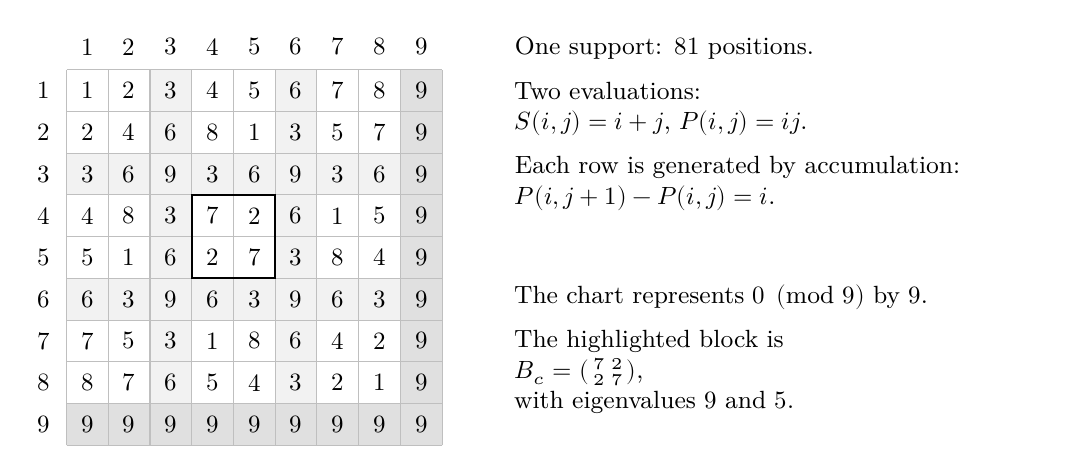
\begin{tikzpicture}[x=.53cm,y=.53cm,font=\small]
\fill[black!5] (1.5,-.5) rectangle (2.5,8.5);
\fill[black!5] (4.5,-.5) rectangle (5.5,8.5);
\fill[black!5] (-.5,2.5) rectangle (8.5,3.5);
\fill[black!5] (-.5,5.5) rectangle (8.5,6.5);
\fill[black!12] (7.5,-.5) rectangle (8.5,8.5);
\fill[black!12] (-.5,-.5) rectangle (8.5,.5);
\foreach \i in {1,...,9}{
 \node at (\i-1,9.05) {\(\i\)};
 \node at (-1.05,9-\i) {\(\i\)};
 \foreach \j in {1,...,9}{
  \pgfmathtruncatemacro{\v}{mod(\i*\j-1,9)+1}
  \node at (\j-1,9-\i) {\(\v\)};
 }
}
\foreach \k in {0,...,9}{
 \draw[black!25] (\k-.5,-.5)--(\k-.5,8.5);
 \draw[black!25] (-.5,\k-.5)--(8.5,\k-.5);
}
\draw[line width=.65pt] (2.5,3.5) rectangle (4.5,5.5);
\node[anchor=west,align=left,text width=6.5cm] at (10,7.2) {One support: \(81\) positions.\\[5pt]Two evaluations:\\ \(S(i,j)=i+j\), \(P(i,j)=ij\).\\[5pt]Each row is generated by accumulation:\\ \(P(i,j+1)-P(i,j)=i\).};
\node[anchor=west,align=left,text width=6.5cm] at (10,1.8) {The chart represents \(0\pmod9\) by \(9\).\\[5pt]The highlighted block is\\ \(B_c=\left(\begin{smallmatrix}7&2\\2&7\end{smallmatrix}\right)\),\\ with eigenvalues \(9\) and \(5\).};
\end{tikzpicture}
\caption{APP multiplication table in positive representatives. Non-unit rows and columns are distinguished by gray shading; the frame identifies the adjacent diagonal block with equal diagonals. The displayed table is an observable of the arithmetic torus; its representation edges do not constitute an intrinsic topological boundary of the torus.}
\label{fig:app}
\end{figure}


\begin{proposition}[Reconstruction of the evaluations]
The two pairs in \eqref{eq:app-levantada} determine \(i+j\) and \(ij\) exactly. The residues alone do not determine these integer evaluations or their quotients.
\end{proposition}
\begin{proof}
The first statement is \eqref{eq:residuo-cociente} applied to each sheet. For the second, \(10=1+9\) and \(19=1+2\cdot9\) have the same residue and different quotients. On the two-dimensional support, positions \((5,5)\) and \((8,2)\) give the same sum and the same product residue, but products \(25=7+18\) and \(16=7+9\). The residue projection identifies data that the lifted evaluation distinguishes.
\end{proof}

\subsubsection{Cayley graph, toroidal topology, and winding number}

The cardinal translations are given, in row and column coordinates, by
\[
 \nu_N=(-1,0),\quad\nu_E=(0,1),\quad
 \nu_S=(1,0),\quad\nu_O=(0,-1),\qquad T_d(x)=x+\nu_d.
\]
The first coordinate increases southwards and the second eastwards. The graph
\[
 \mathscr G_9=\operatorname{Cay}(X_9,\{\nu_N,\nu_E,\nu_S,\nu_O\})
\]
is the two-dimensional cyclic lattice: it has eighty-one vertices and four outgoing oriented edges per vertex. It is a Cayley graph for the \emph{additive} structure of the support. Multiplication of residues has zero divisors and does not turn all APP rows into a multiplicative group.

A cardinal word \(w=d_1\cdots d_r\) and an origin \(x_0\) determine
\[
 x_k=x_0+\sum_{j=1}^k\nu_{d_j}\pmod9.
\]
There are \(81\cdot4^r\) oriented paths of length \(r\), including returns and backtracking. When the path closes, its integer displacement before reduction defines
\begin{equation}
 \operatorname{wind}(w)=\frac19
 \bigl(\#S(w)-\#N(w),\#E(w)-\#O(w)\bigr)\in\ZZ^2.
\end{equation}
Path reversal changes the sign of this vector. Returning to the same residue position therefore does not require the winding to vanish. This is the first example of a distinction that will reappear in phase return: one coordinate may close while another records a nontrivial evolution.

\subsubsection{Transport quotient and cocycle identity}

Let \(s_9:\ZZ/9\ZZ\to D_9\) be the section of positive representatives. The transport quotient associated with additive composition, also called the \emph{carry} in positional arithmetic, is
\[
 c_9(a,b)=\frac{s_9(a)+s_9(b)-s_9(a+b)}9.
\]
The compositional character of this memory is expressed by an exact identity.

\begin{lemma}[Cocycle identity]
For \(a,b,c\in\ZZ/9\ZZ\),
\[
 c_9(a,b)+c_9(a+b,c)=c_9(b,c)+c_9(a,b+c).
\]
\end{lemma}
\begin{proof}
Both sums equal
\[
 \frac{s_9(a)+s_9(b)+s_9(c)-s_9(a+b+c)}9.
\]
Associativity of the sum of lifted representatives requires precisely this additional term when composing in the quotient.
\end{proof}

With positive representatives, this cocycle is not normalized at the identity: \(c_9(0,a)=1\). If \(s_0\) takes representatives in \(\{0,\ldots,8\}\), its normalized carry \(c_0\) satisfies
\[
 c_9(a,b)=c_0(a,b)+\mathbf1_{a=0}+\mathbf1_{b=0}-\mathbf1_{a+b=0}.
\]
The difference is the change of section; it does not alter the cocycle identity. The subsequent decomposition of the calendar into phase and window will use representatives from zero to eight.

The totals of both evaluations distinguish the visible contribution from that retained in the quotient:
\[
 \sum S=810,\quad\sum P=2025,\quad
 \sum\Sigma=405,\quad\sum\Pi=459,
\]
\[
 \sum q^+=45,\qquad\sum q^\times=174.
\]
It follows that
\begin{equation}
 2025-810=(459-405)+9(174-45)=54+9\cdot129.
 \label{eq:defecto-integrado}
\end{equation}
The sum--product difference is not exhausted by the visible defect \(54\). The identity also preserves the quotient defect \(129\). Removing it would change the arithmetic being transported, even if the residue table remained identical.

% BEGIN R27_MG03
\subsubsection{Modulus refinement and preservation of the two readers}
\label{mg03:refinamiento}

Identity \eqref{eq:defecto-integrado} preserves the integer defect
\(1215\) through residue \(54\) and quotient \(129\). Its
generalization requires separate specifications of the reading modulus,
the support size and the number of coordinates. These three operations
produce distinct counting laws from the same APP sheets.

For \(N\geq2\), fix the positive representative
\[
 \rho_N(s)=1+((s-1)\bmod N)\in\{1,\ldots,N\},
 \qquad s=\rho_N(s)+NQ_N(s),\quad Q_N(s)\in\mathbb Z.
\]
On \(\{1,\ldots,N\}^2\), the full-modulus readings are
\(\rho_N(i+j)\) and \(\rho_N(ij)\). Their sums are denoted by
\(S_+^{\mathrm{full}}(N)\) and \(S_\times^{\mathrm{full}}(N)\).

\begin{proposition}[Defect law for an integer modulus]
For every \(N\geq2\),
\begin{align}
 S_+^{\mathrm{full}}(N)&=\frac{N^2(N+1)}2,
 \label{mg03:suma-plena}\\
 S_\times^{\mathrm{full}}(N)&=
 \frac N2\left(N^2+\sum_{i=1}^{N}\gcd(i,N)\right),
 \label{mg03:producto-pleno}\\
 \Delta_N^{\mathrm{full}}&=
 \frac N2\left(\sum_{i=1}^{N}\gcd(i,N)-N\right).
 \label{mg03:defecto-pleno}
\end{align}
\end{proposition}

\begin{proof}
In an additive row, translation by \(i\) permutes the \(N\) residue
classes and their positive representatives. Each row sums to
\(N(N+1)/2\), proving \eqref{mg03:suma-plena}. For a multiplicative
row, let \(g=\gcd(i,N)\). The image of \(j\mapsto ij\pmod N\)
contains the \(N/g\) residue classes divisible by \(g\), and each
has \(g\) preimages. Their positive representatives are
\(g,2g,\ldots,N\), whose sum is
\[
 g\frac{(N/g)(N/g+1)}2=\frac{N(N+g)}{2g}.
\]
Multiplicity \(g\) gives \(N(N+g)/2\) per row. Summation over
\(i\) yields \eqref{mg03:producto-pleno}; subtracting
\eqref{mg03:suma-plena} gives \eqref{mg03:defecto-pleno}.
\end{proof}

\begin{corollary}[Prime-power moduli]
If \(N=p^m\), where \(p\) is prime and \(m\geq1\), then
\begin{equation}
 \sum_{i=1}^{p^m}\gcd(i,p^m)
 =p^m+m(p-1)p^{m-1},\qquad
 \Delta_{p^m}^{\mathrm{full}}
 =\frac{m(p-1)}2p^{2m-1}.
 \label{mg03:primo-potencia}
\end{equation}
\end{corollary}

\begin{proof}
For each \(0\leq k<m\), there are
\(p^{m-k}-p^{m-k-1}\) indices with exact \(p\)-adic valuation
\(k\). Their greatest common divisor with \(p^m\) is \(p^k\),
so this stratum contributes \((p-1)p^{m-1}\). The \(m\) strata
contribute \(m(p-1)p^{m-1}\), whereas the index \(i=p^m\)
contributes \(p^m\). Substitution into \eqref{mg03:defecto-pleno}
gives the second formula.
\end{proof}

The triadic specialization is
\(\Delta_{3^m}^{\mathrm{full}}=m3^{2m-1}\). The first moduli
display both sums together with their difference:
\[
\begin{array}{c|r|r|r}
 N&S_+^{\mathrm{full}}&S_\times^{\mathrm{full}}&\Delta_N^{\mathrm{full}}\\\hline
 3&18&21&3\\
 9&405&459&54\\
 27&10206&10935&729\\
 81&269001&277749&8748
\end{array}
\]

Periodic refinement instead retains \(\rho_9\) and enlarges the
support to \(\{1,\ldots,9r\}^2\), with integer \(r\geq1\). Each pair of residues modulo
nine has \(r^2\) representatives in this support, for both addition
and multiplication. Consequently,
\begin{equation}
 S_+^{\mathrm{per}}(9r;9)=r^2\,405,\quad
 S_\times^{\mathrm{per}}(9r;9)=r^2\,459,\quad
 \Delta^{\mathrm{per}}(9r;9)=r^2\,54.
 \label{mg03:periodico}
\end{equation}
For \(r=3\), the sums are \(3645\) and \(4131\), and the defect
is \(486\). The full-modulus reading at \(27\) produces \(729\)
because it updates both the modulus and its representatives; the periodic
reading produces \(486\) because it retains modulus nine and multiplies
its incidences by nine. In both readings, the divisions
\(i+j=R^++NQ^+\), \(ij=R^\times+NQ^\times\), with the modulus
actually employed, preserve the integer identity at each cell and after
summation. This specifies the datum accompanying each defect.

\subsubsection{Dimensional variation at fixed modulus nine}
\label{mg03:dimension}

A second extension retains the modulus and increases the number of
factors. For \(d\geq1\), let
\[
 \mathcal A_d=\{1,\ldots,9\}^d,\qquad
 \Sigma_d(x)=\rho_9\!\left(\sum_{j=1}^d x_j\right),\qquad
 \Pi_d(x)=\rho_9\!\left(\prod_{j=1}^d x_j\right).
\]

\begin{proposition}[Dimensional count for accumulation and multiplication]
The sums of the two readers over \(\mathcal A_d\) are
\begin{equation}
 S_{+,d}=45\,9^{d-1},\qquad
 S_{\times,d}=9^{d+1}-9(d+3)6^{d-1}.
 \label{mg03:ley-dimensional}
\end{equation}
Therefore,
\begin{equation}
 \frac{S_{\times,d}-S_{+,d}}{9^d}
 =4-(d+3)\left(\frac23\right)^{d-1}
 \longrightarrow4.
 \label{mg03:limite-dimensional}
\end{equation}
\end{proposition}

\begin{proof}
For each fixed choice of the first \(d-1\) coordinates, the final
coordinate traverses every additive residue once. Each positive
representative occurs \(9^{d-1}\) times, and their sum is \(45\);
this proves the additive formula.

For multiplication, distinguish the units \(U=\{1,2,4,5,7,8\}\),
the multiples of three of valuation one \(T=\{3,6\}\), and the
zero representative \(9\). The \(6^d\) words whose factors all
belong to \(U\) distribute their products uniformly over the six
units: fixing \(d-1\) factors leaves a permutation of the group
under multiplication by the last factor. Their contribution is
\(27\,6^{d-1}\).

The words with exactly one factor in \(T\) and all other factors
in \(U\) number \(2d6^{d-1}\). For each position of the singular
factor and each choice of the remaining units, its two possible values
\(3,6\) produce each of the residues \(3,6\) once. Their contribution
is \(9d6^{d-1}\). Every remaining word contains a factor \(9\),
or at least two factors in \(T\), so its product has representative
\(9\). Their number is \(9^d-6^d-2d6^{d-1}\). Thus
\[
 S_{\times,d}=27\,6^{d-1}+9d6^{d-1}
 +9\bigl(9^d-6^d-2d6^{d-1}\bigr),
\]
which simplifies to \eqref{mg03:ley-dimensional}. Dividing by
\(9^d\) and subtracting the additive mean \(5\) gives
\eqref{mg03:limite-dimensional}; the term
\((d+3)(2/3)^{d-1}\) tends to zero.
\end{proof}

Dimension two recovers \(S_{+,2}=405\), \(S_{\times,2}=459\)
and total defect \(54\). The limit \(4\) belongs to the mean
defect under increasing dimension. Total defect, preserved quotient
and dimensional mean are specified readers of APP arithmetic; TRIT
and TPK subsequently transport these data with their orientation,
modulus and mathematical residence.

% END R27_MG03

\subsubsection{Ternary reduction and multiplicative radical}

The ring \(R=\ZZ/9\ZZ\) has unit group \(\{1,2,4,5,7,8\}\) and maximal ideal
\[
 \mathfrak m=(3)=\{0,3,6\},\qquad\mathfrak m^2=0.
\]
Every additive row is a permutation of the nine representatives. A multiplicative row is such a permutation exactly when its index is a unit. Rows three and six contain three repeated values; row nine contains only the representative of the zero class. Thus multiplicative folding already distinguishes the units from the nilpotent sector before any continuous geometry is introduced.

The map \(x\mapsto3x\) has kernel and image both equal to \(\mathfrak m\). It induces an isomorphism of vector spaces over \(\FF_3\),
\[
 R/\mathfrak m\longrightarrow\mathfrak m,\qquad [x]\longmapsto3x,
\]
but not a ring isomorphism. In particular, the visible sequence \(3,6,9\) admits two different readings: its direct reduction modulo three is \(0,0,0\), whereas extracting the factor three and then reducing its internal coordinate gives \(1,2,0\). This second operation preserves a coordinate of the ideal; it is not the same projection as directly reducing the original number.

\subsubsection{Latin realization of the additive evaluation}

The difference between the two evaluations can also be expressed through
operators. Let \((e_r)_{r\in\ZZ/9\ZZ}\) be the orthonormal basis of \(\CC^9\).
The assignment \(v_{ab}=e_{a+b}\) produces an orthonormal basis in every row
and column. The projectors \(P_{ab}=v_{ab}v_{ab}^{*}\) satisfy
\[
 \sum_bP_{ab}=I_9=\sum_aP_{ab},\qquad P_{ab}^2=P_{ab}.
\]
Indeed, each translation \(b\mapsto a+b\) permutes the nine residues.
This yields a realization of a Latin square by rank-one projectors,
in the terminology of quantum Latin squares
\cite{mustovicary,delascuevas2023}. This construction starts from the
additive sheet already defined and makes explicit the map to its operator representation.

The multiplicative evaluation preserves different content: for \(a=3\), the
vectors \(e_{3b}\) repeat the residues \(0,3,6\), and
\[
 \sum_{b\in\ZZ/9\ZZ}|e_{3b}\rangle\langle e_{3b}|
 =3\bigl(|e_0\rangle\langle e_0|+|e_3\rangle\langle e_3|
                    +|e_6\rangle\langle e_6|\bigr).
\]
The multiplicity is recorded in the operator and characterizes the multiplicative
radical. Thus the toroidal support, the Latin property, and the operator
resolution of the identity are properties requiring different definitions.
The quantum magic squares studied by De las Cuevas, Drescher, and Netzer
require positive entries and row and column sums equal to the identity;
their theory also distinguishes dilations with commuting entries\cite{delascuevas2020}.
This reference provides a precise language for comparing realizations of APP.

\subsection{TRIT: orientation and quadratic regimes}

\begin{definition}[Ternary signature and local lift]
The TRIT signature uses the balanced identification
\[
 \FF_3\longrightarrow\TRIT,\qquad 0\mapsto0,\quad1\mapsto+1,\quad2\mapsto-1.
\]
For \(n\in\ZZ\), its lift preserves \(n=r+3c\), where \(r\in\TRIT\) and \(c\in\ZZ\). In a transition of bounded local amplitude, the three states \((0,-1),(0,0),(0,+1)\) may exhibit the same zero residue and different carries.
\end{definition}

The signature does not replace the trajectory. A zero residue does not mean an absence of orientation, phase, or quotient information. Nor does it introduce a physical quantity by itself. Its function is to distinguish algebraically the transport classes that will be realized next.

\subsubsection{Three quadratic regimes and a common exponential}

Once the ternary signature has been obtained, its quadratic realization is defined by
\begin{equation}
 \mathbb A_\tau=\RR[X]/(X^2+\tau),\qquad \tau\in\TRIT.
 \label{eq:algebras-trit}
\end{equation}
If \(J_\tau\) is the class of \(X\), then \(J_\tau^2=-\tau I\). The structure distinguishes the elliptic type \(\tau=+1\), the parabolic type \(\tau=0\), and the hyperbolic type \(\tau=-1\). The real realization does not generate the signature: it expresses the types already produced by oriented reduction.

\begin{proposition}[Exponentiation of the three types]
In each algebra \eqref{eq:algebras-trit},
\begin{equation}
 \exp(tJ_\tau)=C_\tau(t)I+S_\tau(t)J_\tau,
\end{equation}
where
\[
 C_\tau(t)=\sum_{n\ge0}\frac{(-\tau)^nt^{2n}}{(2n)!},\qquad
 S_\tau(t)=\sum_{n\ge0}\frac{(-\tau)^nt^{2n+1}}{(2n+1)!}.
\]
The three realizations are
\[
 \begin{array}{c|c|c}
 \tau&J_\tau^2&\exp(tJ_\tau)\\\hline
 +1&-I&\cos t\,I+\sin t\,J_\tau\\
 0&0&I+tJ_\tau\\
 -1&I&\cosh t\,I+\sinh t\,J_\tau.
 \end{array}
\]
\end{proposition}
\begin{proof}
Separating the even and odd terms of the exponential series and substituting \(J_\tau^{2n}=(-\tau)^nI\) and \(J_\tau^{2n+1}=(-\tau)^nJ_\tau\) gives the formulas. For \(\tau=0\), all terms of degree at least two vanish. In the other two cases, the trigonometric or hyperbolic series are recovered.
\end{proof}

The exponential is common to all three regimes: it is not assigned exclusively to the parabolic branch. The invariants
\[
 C_\tau(t)^2+\tau S_\tau(t)^2=1
\]
follow from \(\exp(tJ_\tau)\exp(-tJ_\tau)=I\). The same algebraic principle preserves unity through realizations that differ in their quadratic type.

In the hyperbolic regime, \(P_\pm=(I\pm J_{-1})/2\) are complementary projectors and
\[
 \exp(tJ_{-1})=e^tP_++e^{-t}P_-.
\]
Growth and contraction appear jointly in two eigendirections. In the elliptic regime, the parameter describes a rotation; in the parabolic regime, a nilpotent translation. The temporal interpretation adopted by HMT associates \(+1\) with return with memory, \(0\) with the threshold, and \(-1\) with bidirectional opening. This interpretation requires an ordering of the parametrization; it does not add a fourth algebraic type.

% Cumulative TRIT extension; inserted before the regime figure.
% It neither replaces nor removes the preceding development.
\subsubsection{Balanced division and composition of lifts}
\label{trit-ampl-div-balanceada}

Ternary reduction expresses an integer evaluation of APP through a visible
coordinate and a prolongation coordinate. Its function is not merely to
abbreviate the notation for an integer: it provides a composition rule
determining how the quotient changes when evaluations are added or multiplied.
The balanced choice also makes the compatibility of this rule with sign
reversal explicit.

\begin{definition}[Balanced ternary coordinates]
\label{trit-ampl-def-coordenadas}
For \(n\in\mathbb Z\), let
\[
 q_3(n)=\left\lfloor\frac{n+1}{3}\right\rfloor,\qquad
 r_3(n)=n-3q_3(n).
\]
The map
\[
 \mathcal B:\mathbb Z\longrightarrow\TRIT\times\mathbb Z,\qquad
 n\longmapsto(r_3(n),q_3(n))
\]
is called the balanced ternary decomposition. Its inverse is
\(\mathcal L(r,c)=r+3c\).
\end{definition}

Indeed, \(r_3(n)\in\{-1,0,+1\}\). If two pairs represent the same integer,
\(r+3c=s+3d\), then \(r-s\) is a multiple of \(3\) and belongs to the interval
\([-2,2]\); necessarily \(r=s\) and \(c=d\). The representation is therefore
unique. Division can be repeated on \(q_3(n)\), so that each level preserves
the data needed to reconstruct the preceding one. The quotient is not a
perturbation of the residue: it is its complementary coordinate.

The signature obtained from an evaluation \(F\), with \(F=S\) or \(F=P\) in APP,
is \(r_3\circ F\). When reduction acts on the phase cursor, the same balanced
section produces the classes \(\{1,4,7\}\), \(\{2,5,8\}\), and
\(\{3,6,9\}\), with values \(+1,-1,0\). The TPK selector defined below
uses these classes to determine the operating mode.
Reading an evaluation and selecting a mode thus share the same ternary
reduction, but have different domains and functions.

\Needspace{16\baselineskip}
\begin{proposition}[Arithmetic of balanced pairs]
\label{trit-ampl-prop-aritmetica}
Let \(n=r+3c\) and \(m=s+3d\), with \(r,s\in\TRIT\). Define
\[
 \chi(r,s)=\frac{r+s-r_3(r+s)}3.
\]
Integer operations are transported to the pairs by
\begin{align}
 (r,c)\boxplus(s,d)
 &=\bigl(r_3(r+s),c+d+\chi(r,s)\bigr),
 \label{trit-ampl-eq-suma}\\
 (r,c)\boxtimes(s,d)
 &=\bigl(rs,rd+sc+3cd\bigr).
 \label{trit-ampl-eq-producto}
\end{align}
The map \(\mathcal L\) preserves both operations.
\end{proposition}
\begin{proof}
The equality \(r+s=r_3(r+s)+3\chi(r,s)\) gives
\[
 n+m=r_3(r+s)+3\bigl(c+d+\chi(r,s)\bigr).
\]
On the other hand,
\[
 nm=rs+3(rd+sc+3cd).
\]
Since the product of two balanced representatives again belongs to
\(\{-1,0,+1\}\), it requires no additional residue reduction. Uniqueness
of the decomposition proves both formulas.
\end{proof}

For example, \(2=(-1)+3\) and \(4=1+3\). Their sum and product are reconstructed
as
\[
 (-1,1)\boxplus(1,1)=(0,2),\qquad
 (-1,1)\boxtimes(1,1)=(-1,3).
\]
The resulting evaluations are \(6\) and \(8\). Adding the quotients suffices
in this additive example; the product involves the cross terms
\(rd\), \(sc\), and \(3cd\). The discrepancy between the two operations
also resides in the prolongation coordinate, not only in the residue.

The term \(\chi\) is a cocycle of the balanced section. If
\(r\oplus s=r_3(r+s)\), it satisfies
\[
 \chi(r,s)+\chi(r\oplus s,t)
 =\chi(s,t)+\chi(r,s\oplus t).
\]
Both sides represent the quotient of the same sum of three integers.
This identity ensures that regrouping the operations does not change the
reconstructed evaluation. At the same time, projection onto the first
component suppresses this accounting: \(1+1=-1+3\), whereas the residue
reading retains only \(-1\). The information removed is determined,
in this case, by \(\chi(1,1)=1\).

The relation with modulus \(9\) preserves a second discrete scale.
The map
\[
 \beta:\TRIT\times\mathbb F_3\longrightarrow\mathbb Z/9\mathbb Z,
 \qquad (r,\bar c)\longmapsto r+3c\pmod9
\]
is well defined and bijective. Changing the representative of \(\bar c\)
adds a multiple of \(9\); conversely, equality of images fixes
\(r\) first, by reduction modulo \(3\), and then \(\bar c\). Addition
transported by this bijection contains the term
\(\chi(r,s)\) from \eqref{trit-ampl-eq-suma}, now reduced modulo \(3\).
Thus the two ternary levels do not compose by independent coordinatewise
addition: normalization of the first level modifies the second.

In particular, the classes \(3\), \(6\), and \(0\) of
\(\mathbb Z/9\mathbb Z\) have first component \(0\), but second components
\(1\), \(2\), and \(0\), respectively. The distinction already observed
between direct reduction and extraction of the ideal coordinate appears
as a property of \(\beta\). Preserving this coordinate prevents the zero
residue sector from being artificially collapsed into a single position.
Modulus \(1000\), used later to organize decimal blocks,
serves a different positional-representation function; its quotient is
preserved through the corresponding division. A change of base preserves
the integer when it retains residue and quotient, whereas coincidence of
residues in different bases does not by itself identify their transport states.

\Needspace{11\baselineskip}
\subsubsection{Inversion, residue class, and non-visible coordinates}
\label{trit-ampl-inversion}

Additive inversion lifts unambiguously:
\[
 \mathcal B(-n)=(-r_3(n),-q_3(n)).
\]
In particular, \(3\), \(0\), and \(-3\) have coordinates
\((0,1)\), \((0,0)\), and \((0,-1)\). They share a zero signature but
represent different evaluations. In a transition restricted to a quotient
of maximum amplitude \(1\), these are the three possibilities of the
visible fiber over zero; in a general integer lift, that fiber contains
all pairs \((0,c)\), with \(c\in\mathbb Z\).

The quotient coordinate recovers the evaluated integer, but does not by
itself recover the trajectory that produced it. Two APP paths may share
evaluation, residue, and quotient while differing in orientation, sequence
of modes, or winding. Thus decomposition \(\mathcal B\) is integrated into
the transport state rather than replacing it. The arithmetic memory of a
division and the memory of a trajectory are related coordinates, not synonyms.

For a signature sequence of length \(n\), oriented reversal is
\[
 C_{\rm rev}(\tau_1,\ldots,\tau_n)
   =(-\tau_n,\ldots,-\tau_1).
\]
Applying it twice restores the sequence. The operation reverses the order
of positions and the sign of each signature; it preserves the length and
the zero positions in reversed order. In the adopted parametrization,
it interchanges return with memory, associated with \(+1\), and bidirectional
opening, associated with \(-1\), while retaining the threshold \(0\).
Transport of the remaining trajectory data is specified by the corresponding
TPK involution.

This signature reversal must be distinguished from conjugation within a
quadratic algebra. The former may change the type \(\tau\); the latter,
constructed below, acts within a type already fixed. This distinction
prevents attributing an algebraic equivalence between different regimes
to a sign reversal.

\subsubsection{Quadratic product, conjugation, and algebraic norm}
\label{trit-ampl-norma}

An element of \(\mathbb A_\tau\) has a unique expression \(aI+bJ_\tau\).
The relation \(J_\tau^2=-\tau I\) determines its product:
\begin{equation}
 (aI+bJ_\tau)(cI+dJ_\tau)
   =(ac-\tau bd)I+(ad+bc)J_\tau.
 \label{trit-ampl-producto-cuadratico}
\end{equation}
This is a real realization of the type already selected. The coordinates
\(a,b\) are not APP residues, and the product
\eqref{trit-ampl-producto-cuadratico} does not replace
\eqref{trit-ampl-eq-producto}; it expresses another operation in the
declared quadratic codomain.

\begin{definition}[Conjugation and algebraic norm]
\label{trit-ampl-def-norma}
Conjugation of type \(\tau\) and its algebraic norm are
\[
 \overline{aI+bJ_\tau}=aI-bJ_\tau,\qquad
 N_\tau(aI+bJ_\tau)=a^2+\tau b^2.
\]
\end{definition}

\begin{proposition}[Multiplicativity and invertibility]
\label{trit-ampl-prop-norma}
For \(z,w\in\mathbb A_\tau\),
\[
 z\bar z=N_\tau(z)I,\qquad
 N_\tau(zw)=N_\tau(z)N_\tau(w).
\]
Moreover, \(z\) is invertible if and only if \(N_\tau(z)\ne0\), in which case
\[
 z^{-1}=\frac{\bar z}{N_\tau(z)}.
\]
\end{proposition}
\begin{proof}
The product of \(aI+bJ_\tau\) and \(aI-bJ_\tau\) is
\((a^2+\tau b^2)I\). Conjugation is multiplicative and the algebra is
commutative, so that
\((zw)\overline{zw}=(z\bar z)(w\bar w)\). If the norm does not vanish,
the stated formula supplies the inverse. Conversely, if \(zw=I\),
multiplicativity implies \(N_\tau(z)N_\tau(w)=1\).
\end{proof}

The quadratic form \(N_\tau\) is positive definite only in the elliptic type.
For \(\tau=0\), it equals \(a^2\), and the element \(J_0\) is nonzero although
its square and norm are zero. For \(\tau=-1\), it equals \(a^2-b^2\);
the nonzero elements \(I+J_{-1}\) and \(I-J_{-1}\) have zero norm and
their product vanishes. Here the algebraic norm is a multiplicative
quadratic form: it does not presuppose a positive vector-space norm.

The three types admit faithful realizations by
\[
 aI+bJ_\tau\longmapsto
 \begin{pmatrix}a&-\tau b\\b&a\end{pmatrix}.
\]
The determinant of this matrix is \(N_\tau(aI+bJ_\tau)\).
The complex structure, the dual-number structure, and the split real
structure are thus represented by a single matrix expression.
Each preserves its own law and zero divisors. The form of signature
\((1,1)\) in the last case admits a Lorentzian interpretation in dimension
\(1+1\); identification of a physical metric additionally requires a
specific space, field, and transport rule.

\subsubsection{Multiplicative conservation and composition of evolutions}
\label{trit-ampl-evoluciones}

The exponential already obtained belongs to the set of norm-one elements:
\[
 N_\tau\bigl(\exp(tJ_\tau)\bigr)=1.
\]
This conservation persists under composition of parameters. Indeed, all
factors are functions of the same generator, and
\[
 \exp(tJ_\tau)\exp(sJ_\tau)=\exp((t+s)J_\tau).
\]
Comparing the two components gives the addition laws
\begin{align}
 C_\tau(t+s)&=C_\tau(t)C_\tau(s)-\tau S_\tau(t)S_\tau(s),\\
 S_\tau(t+s)&=S_\tau(t)C_\tau(s)+C_\tau(t)S_\tau(s).
\end{align}
Conjugation changes \(t\) to \(-t\) and coincides with inversion within
this subgroup. It does not change \(\tau\): it reverses an evolution of
the chosen regime.

In the elliptic type, the preserved form is \(a^2+b^2\), and the exponential
trajectory traverses the unit-norm circle. In the hyperbolic type, the
eigencoordinates are \(u=a+b\), \(v=a-b\), with \(uv=N_{-1}(z)\).
The exponential gives
\[
 (u,v)=(e^t,e^{-t}),\qquad uv=1.
\]
Growth of one coordinate is accompanied by contraction of the other.
Conservation expresses a relation between the two coordinates; it does
not assert that each remains constant.

In the parabolic type,
\[
 (I+tJ_0)(I+sJ_0)=I+(t+s)J_0,\qquad
 (I+tJ_0)^{-1}=I-tJ_0.
\]
The evolution does not stop because \(J_0^2=0\). Nilpotency removes terms
of order at least two, but preserves the linear term that transports
the parameter. The visible symbol \(0\), the zero element of the algebra,
and the nonzero generator \(J_0\) are distinct. This distinction is
necessary to describe the threshold without identifying it with an absence
of state or dynamics.

\begin{proposition}[Composition of affine coordinates]
\label{trit-ampl-prop-pendientes}
In the chart where the scalar component does not vanish, represent a
direction by \(I+uJ_\tau\). If \(1-\tau uv\ne0\), the direction of its
product with \(I+vJ_\tau\) has coordinate
\[
 u\star_\tau v=\frac{u+v}{1-\tau uv}.
\]
\end{proposition}
\begin{proof}
We have
\[
 (I+uJ_\tau)(I+vJ_\tau)
   =(1-\tau uv)I+(u+v)J_\tau.
\]
Dividing by the scalar component gives the stated expression.
\end{proof}

The affine chart preserves the ratio of components, not the scalar factor
divided out. When \(1-\tau uv=0\), the product must be examined before
changing charts: it may have a well-defined direction with zero scalar
component, or be the zero element in the presence of zero divisors.
The composition law still belongs to the full algebra; a coordinate
singularity does not automatically imply a singularity of the object.
This formula will reappear in the elliptic regional reading. Its use
requires retaining the denominator and, where applicable, the normalization factor.

\subsubsection{Transport of type and subsequent realizations}
\label{trit-ampl-puentes}

The algebras \(\mathbb A_{+1}\), \(\mathbb A_0\), and
\(\mathbb A_{-1}\) are not isomorphic as unital real algebras.
The first is a field; the second contains a nonzero nilpotent; the
third has nontrivial idempotents and is isomorphic to
\(\mathbb R\times\mathbb R\). Thus a change of signature organizing a
route cannot be interpreted as an undifferentiated isomorphism between
the three realizations. The TPK preserves the regime index, the domains,
and the effective operator acting at each transition.

In the electron chapter, the pair of projections of the APP sheets
produces a normalized commutator whose square is \(-I\). The same block
contains an involution of square \(I\) and two nilpotent directions.
The joint realization will be proved for that concrete pair of projections;
the preceding classification explains why the three quadratic relations
can appear within one matrix algebra without being identified with one another.

In the exceptional prolongation, the Paley matrix reduced modulo \(3\)
satisfies \(A_W^2=-I_6\). This relation endows the ternary space with
a structure of dimension \(3\) over \(\mathbb F_9\). Its connection to
a real operator root is expressed through the integral presentation
\[
 \mathbb Z[u]/(u^2+1).
\]
Base changes to \(\mathbb F_3\) and \(\mathbb R\) produce representations
of the same relation. Each retains its characteristic, dimension, and
incidence information. Developing the respective operators establishes
the connection, not equality of their cardinalities.

Norm-one conservation consequently describes the quadratic realizations
of evolutions. Conservation of quotients, orientation, and trajectory
belongs to the transported arithmetic state. Both properties participate
in the construction, with different functions: one determines the identities
of the representations; the other makes it possible to compose, reconstruct,
and prolong the operations that give rise to them.


\begin{figure}[htbp]
\centering
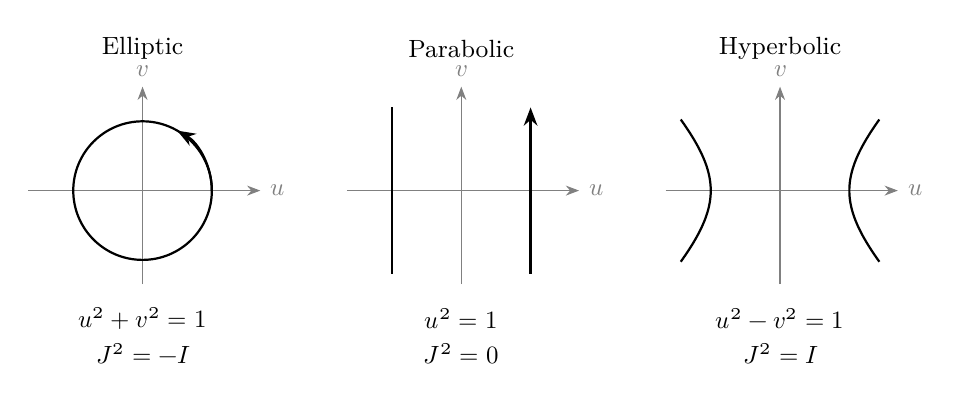
\begin{tikzpicture}[scale=.88,>=Stealth,font=\small]
\foreach \c/\titulo in {0/{Elliptic},4.6/{Parabolic},9.2/{Hyperbolic}}{
\begin{scope}[xshift=\c cm]
\draw[->,gray] (-1.65,0)--(1.7,0) node[right] {\(u\)};
\draw[->,gray] (0,-1.35)--(0,1.5) node[above] {\(v\)};
\node at (0,2.05) {\titulo};
\end{scope}}
\draw[thick] (0,0) circle[radius=1];
\draw[->,thick] (1,0) arc[start angle=0,end angle=60,radius=1];
\node at (0,-1.85) {\(u^2+v^2=1\)};
\node at (0,-2.35) {\(J^2=-I\)};
\draw[thick] (3.6,-1.2)--(3.6,1.2);
\draw[->,thick] (5.6,-1.2)--(5.6,1.2);
\node at (4.6,-1.85) {\(u^2=1\)};
\node at (4.6,-2.35) {\(J^2=0\)};
\draw[thick,domain=-.9:.9,samples=50] plot ({9.2+cosh(\x)},{sinh(\x)});
\draw[thick,domain=-.9:.9,samples=50] plot ({9.2-cosh(\x)},{sinh(\x)});
\node at (9.2,-1.85) {\(u^2-v^2=1\)};
\node at (9.2,-2.35) {\(J^2=I\)};
\end{tikzpicture}
\caption{Quadratic realizations of TRIT. For
\(J_\tau=\left(\begin{smallmatrix}0&-\tau\\1&0\end{smallmatrix}\right)\),
the exponential preserves \(u^2+\tau v^2\). Parabolic degeneration
preserves \(u\) and transports \(v\) linearly. The three diagrams represent
orbits of quadratic forms; their geometric type corresponds to the
algebraic relation of the generator.}
\label{fig:trit-regimenes}
\end{figure}


\newpage
\subsection{TPK: Topological Phase Kernel}

The dynamics uses the phase selector
\[
 M_{\rm ph}(r)=
 \begin{cases}
 +1,&r\in\{1,4,7\},\\
 -1,&r\in\{2,5,8\},\\
 0,&r\in\{3,6,9\}.
 \end{cases}
\]
Its value determines which evaluation operates. Cardinal transport moves the corresponding cursor; the record preserves the previous value, the new quotient, the orientation, and the transition. Selection and transport are therefore different functions: a ternary sign is not a displacement on the torus.

We shall denote by \(\widehat X\) the space of arithmetic states with trajectory memory. An element contains the positions and directions of both cursors, the active mode, the TRIT signature, the phase, the residues and quotients of both evaluations, the carries, the constructed prefix, and the boundary data. When a refinement cylinder is introduced, it forms part of the state. This notation avoids replacing the object by a reduced version that retains only the visible symbol.

\begin{definition}[TPK update]
Let \(\mathsf{Sel}_t\) be mode selection through \(M_{\rm ph}\), \(\mathsf{Tra}_t\) the lifted cardinal transport, and \(\mathsf{Mem}_t\) the record update. The transition is
\begin{equation}
 \mathcal U_t=\mathsf{Mem}_t\circ\mathsf{Tra}_t\circ\mathsf{Sel}_t.
 \label{eq:actualizacion}
\end{equation}
Each application preserves the fields it does not modify and updates the remaining fields by Euclidean division and trajectory concatenation.
\end{definition}

The notation \eqref{eq:actualizacion} expresses the order of composition; it does not replace the effective rules. The following section specifies its finite two-cursor realization completely. Prolongation will then be obtained not by erasing its memory and repeating the first emission, but by transporting the prefixes and their compatible boundaries. Thus APP supplies the evaluations, TRIT distinguishes their regimes, and TPK composes their evolution.

% Expository recovery from the TPK kernel's source owners.
% Provenance and preservation controls are documented in technical/TPK_INTEGRACION.md.
% This file expands the TPK section; it does not replace extension.tex or generacion.tex.

\subsubsection{Dynamic state, observables, and operational dependencies}
\label{tpk-int:estado}

The Topological Phase Kernel organizes the evolution of the two APP sheets
with the orientation determined by TRIT. Its definition comprises the state
on which it acts, the transition rules, and the relations that make
prolongations compatible. Equation \eqref{eq:actualizacion} acquires operational
content when the coordinates received and modified by each factor are specified.
Position belongs to the toroidal support; phase belongs to the calendar;
orientation determines transport; quotients record the arithmetic evaluation
before reduction. These coordinates are related through the transition and
retain different mathematical functions.

The observable projection of a state is
\begin{equation}
 q=(x_+,d_+,x_\times,d_\times,\theta)
 \in\mathcal Q_{\rm obs}
 :=(X_9\times\mathcal D)^2\times\Theta_{108},
 \qquad \mathcal D=\{N,E,S,O\},\quad
 \Theta_{108}=\ZZ/108\ZZ.
 \label{tpk-int:qobs}
\end{equation}
The subscripts distinguish the additive and multiplicative cursors. The
fibers of complete states over \(q\) preserve the ordered trajectory, the
integer evaluations of both sheets, their residues and quotients, and the
orientation and boundary records. A precision prolongation adds the prefix
and the compatible cylinder. Thus two states with the same projection
\(q\) may retain different records.

Operational dependencies have three levels. At the local level, the selector
activates a sheet, transport changes its position, and the update computes
the new arithmetic coordinates. At the trajectory level, these transitions
compose and retain the records of preceding steps. At the refinement level,
extension relations determine which continuation preserves the predecessor's
prefix, signature, and boundary. The finite calendar describes the phase
of these operations; holonomy describes their composition on the history.

\subsubsection{Tritic selection and lifted cardinal transport}
\label{tpk-int:seleccion}

Let \(\bar\theta\in\{0,\ldots,107\}\) be the calendar representative.
The operating phase and the dodecaphase sector are
\begin{equation}
 r(\theta)=1+(\bar\theta\bmod9),\qquad
 \beta(\theta)=\left[\left\lfloor\frac{\bar\theta}{9}\right\rfloor\right]_{12}.
 \label{tpk-int:fase}
\end{equation}
The previously defined selector may be written \(\varepsilon_9=M_{\rm ph}\).
Its value vector in the ordered chart of \(D_9\) is
\[
 m_{\rm ph}=(1,-1,0,1,-1,0,1,-1,0).
\]
The function \(M_{\rm ph}:D_9\to\TRIT\) and this vector are two
presentations of the same selector, with their respective domains.

Define the activation indicators
\[
 a_+(\theta)=\mathbf1_{\{1,4,7\}}(r(\theta)),\qquad
 a_\times(\theta)=\mathbf1_{\{2,5,8\}}(r(\theta)).
\]
Cursor transport is then
\begin{equation}
 x_+'=x_++a_+(\theta)\nu_{d_+},\qquad
 x_\times'=x_\times+a_\times(\theta)\nu_{d_\times}
 \quad\text{in }X_9.
 \label{tpk-int:cursores}
\end{equation}
In phases \(3,6,9\), both positions remain unchanged; the neutral event
forms part of the chronology and its record. Cardinal directions determine
the vectors \(\nu_d\), whereas the phase signature determines which
vector is applied.

The integer lift preserves boundary crossing. If
\(s:X_9\to D_9^2\) chooses positive representatives and
\(x'=x+a\nu_d\), with \(a\in\{0,1\}\), define
\begin{equation}
 b_d(x,a)=\frac{s(x)+a\nu_d-s(x')}{9}\in\ZZ^2.
 \label{tpk-int:borde}
\end{equation}
Divisibility by \(9\) follows from equality in \(X_9\).
If \(z\in\ZZ^2\) records previous crossings, the update is
\(z'=z+b_d(x,a)\). Thus
\[
 s(x')+9z'=s(x)+9z+a\nu_d.
\]
The integer transport data remain reconstructible after the position
has been reduced on the torus.

\begin{proposition}[Conservation of lifted displacement]
\label{tpk-int:prop-desplazamiento}
For a cardinal trajectory of \(n\) steps, with activation indicators
\(a_t\),
\[
 s(x_n)+9z_n=s(x_0)+9z_0+
 \sum_{t=0}^{n-1}a_t\nu_{d_t}.
\]
The same equality is preserved under concatenation of two compatible trajectories.
\end{proposition}
\begin{proof}
The one-step identity is \eqref{tpk-int:borde}. Summing it over the
\(n\) steps cancels the intermediate coordinates. Splitting the summation
interval into two segments produces exactly the concatenation law.
For a closed trajectory, the difference \(z_n-z_0\) is the previously
defined winding number.
\end{proof}

The same principle governs APP evaluations. If a sheet takes the integer
value \(N_t\), its record simultaneously preserves
\(N_t=R_t+9q_t\). The difference between two steps satisfies
\[
 N_{t+1}-N_t=(R_{t+1}-R_t)+9(q_{t+1}-q_t).
\]
Spatial-crossing memory \(z_t\) and arithmetic quotient \(q_t\)
have different definitions; preserving them jointly maintains the
geometric and arithmetic provenance of every transition.

\subsubsection{Two-cursor chronology and composite returns}
\label{tpk-int:cronologia}

The cardinal involution \(\jmath\) interchanges \(N\) with \(S\) and
\(E\) with \(O\). After applying \eqref{tpk-int:cursores}, both
directions are reversed at the end of a block of \(27\) steps.
Writing
\[
 h(\theta)=\mathbf1_{\{0,27,54,81\}}
             ((\bar\theta+1)\bmod108),
\]
the complete rule on the observable projection is
\begin{equation}
 F_{\rm obs}(q)=
 \bigl(x_+',\jmath^{h(\theta)}d_+,
       x_\times',\jmath^{h(\theta)}d_\times,
       \theta+1\bigr).
 \label{tpk-int:fobs}
\end{equation}
The reading that forms the emission uses the positions before transport,
according to the explicit recurrence in Section~\ref{sec:extension}.
The observable update and emission therefore compose in a fixed order.

\begin{proposition}[Reversibility and period of the observable calendar]
\label{tpk-int:periodo}
The map \(F_{\rm obs}\) is a permutation of
\(\mathcal Q_{\rm obs}\) and satisfies \(F_{\rm obs}^{108}=I\).
Within a block of \(54\) steps, positions and directions are restored;
the coordinate in \(\Theta_{108}\) advances by \(54\).
\end{proposition}
\begin{proof}
Given the final state, the preceding phase is first recovered by subtracting
one in \(\Theta_{108}\). That phase determines whether directions were
reversed and which cursor moved. Applying the corresponding involution
and subtracting the cardinal vector uniquely recovers the initial state.

Each interval of \(27\) steps contains nine activations of each cursor.
The following block preserves the activations and reverses the directions,
so the integer displacements cancel over \(54\) steps. The rule has
period \(54\) in its position and orientation increments; the same
cancellation holds for any calendar origin. After \(108\) steps,
\(\theta\) is also restored.
\end{proof}

We reserve
\[
 \mathcal K_{27}=F_{\rm obs}^{27}:
 \mathcal Q_{\rm obs}\longrightarrow\mathcal Q_{\rm obs}
\]
for the iterate of \(27\) transitions. Its fourth iterate is the
identity on the observable state defined in \eqref{tpk-int:qobs}.
Projecting history onto the calendar makes this finite check possible.
The trajectory record, its evaluations, and the new prefixes remain in
the dynamic state on which \(\mathcal U_t\) acts; observable equality
does not reinitialize them.

\subsubsection{Affine memory transport and composition of states}
\label{tpk-int:memoria}

The observable projection admits fibers of arithmetic and geometric data.
Over a configuration \(q\), we write a state in the form
\[
 x=(q,o,h,c,\sigma,C,b,\lambda).
\]
Here \(o\) preserves orientation and sheet; \(h\), residues and
quotients; \(c\), additive transport memory; \(\sigma\), the boundary
signature; \(C\), the precision cylinder; \(b\), its boundary label;
and \(\lambda\), the recorded trajectory. The signature is determined
by a map
\[
 \operatorname{Sig}_q:
 \mathsf H_q\times\mathsf C_q\times\mathsf{Hist}_q
 \longrightarrow\mathsf S_q,
 \qquad \sigma=\operatorname{Sig}_q(h,c,\lambda).
\]
The symbols \(\mathsf H_q,\mathsf C_q,\mathsf{Hist}_q\), and
\(\mathsf S_q\) denote, respectively, the sets of residue--quotient
data, the abelian transport-memory group, the recorded trajectories,
and the boundary signatures. Realizations of this signature are specified
component by component in the regional and terminal constructions.
This dependence prevents treating the signature as a free parameter
once the data producing it are fixed.

The elementary residue--quotient chart is explicit. For
\(n\in\ZZ\), let
\[
 r=1+((n-1)\bmod9),\qquad u=\frac{n-r}{9}.
\]
Then \(n=r+9u\), with \(r\in D_9\) and \(u\in\ZZ\).
Uniqueness follows because two representatives in \(D_9\) congruent
modulo \(9\) are equal. This chart supplies local integer reconstruction.
The precision towers additionally incorporate the truncation maps and
cylinders developed in \ref{sec:extension} and \ref{sec:generacion}.

Let \(\gamma:q\to q'\) be an observable trajectory. Fiber transport
is expressed through maps
\[
 \mathsf H(\gamma):\mathsf H_q\to\mathsf H_{q'},\qquad
 \mathsf C(\gamma):\mathsf C_q\to\mathsf C_{q'},\qquad
 \mathsf{Hist}(\gamma):\mathsf{Hist}_q\to\mathsf{Hist}_{q'}.
\]
The maps respect identities and composition, and
\(\mathsf C(\gamma)\) is an abelian-group homomorphism.
The increment \(k_{\rm tr}(\gamma)\in\mathsf C_{q'}\) satisfies
\begin{equation}
 \begin{split}
 k_{\rm tr}(\operatorname{id}_q)&=0,\\
 k_{\rm tr}(\gamma_2\circ\gamma_1)
 &=k_{\rm tr}(\gamma_2)+
   \mathsf C(\gamma_2)k_{\rm tr}(\gamma_1).
 \end{split}
 \label{tpk-int:cociclo}
\end{equation}
Here \(k_{\rm tr}\) denotes the transport cocycle;
the rational coordinate \(\kappa\) of record \(K\) retains
its notation in the dodecaphase-closure chapter.

Transportable coordinates are updated by
\begin{equation}
 \begin{aligned}
 h'&=\mathsf H(\gamma)h,&
 c'&=\mathsf C(\gamma)c+k_{\rm tr}(\gamma),\\
 \lambda'&=\gamma\circ\lambda,&
 \sigma'&=\operatorname{Sig}_{q'}(h',c',\lambda').
 \end{aligned}
 \label{tpk-int:accion-memoria}
\end{equation}
The second equation is an affine action: the linear term transports
previous memory and the cocycle adds the increment produced by the
trajectory. In the spatial-crossing realization for each cursor separately,
\(\mathsf C(\gamma)=I\) and \(k_{\rm tr}(\gamma)\) is the sum
of the vectors in \eqref{tpk-int:borde}. This concrete instance connects
the abstract law with the cardinal operations already defined.

\begin{proposition}[Compatibility of the update with concatenation]
\label{tpk-int:composicion-memoria}
Updating by \eqref{tpk-int:accion-memoria} along
\(\gamma_1\), followed by updating along \(\gamma_2\),
coincides with updating along \(\gamma_2\circ\gamma_1\).
\end{proposition}
\begin{proof}
For the affine coordinate, two updates give
\[
 c''=\mathsf C(\gamma_2)\mathsf C(\gamma_1)c
       +\mathsf C(\gamma_2)k_{\rm tr}(\gamma_1)
       +k_{\rm tr}(\gamma_2).
\]
Functoriality of \(\mathsf C\) and
\eqref{tpk-int:cociclo} turn this expression into
\(\mathsf C(\gamma_2\circ\gamma_1)c+
k_{\rm tr}(\gamma_2\circ\gamma_1)\).
The statement for \(h\) follows from composition of
\(\mathsf H\), and that for \(\lambda\) from associativity
of trajectories. The final signature agrees because it is evaluated
on the same three reconstructed coordinates.
\end{proof}

The cylinder and its boundary complete this law through the relations
\(\operatorname{Ext}_\gamma\), defined in
\ref{tpk-int:bidireccionalidad}. Their elements determine which of
the preceding updates preserve an admissible prolongation.
States, together with the triples \((\gamma,x,x')\) admitted by
these relations, form a category over observable trajectories:
\[
 (\gamma_2,x',x'')\circ(\gamma_1,x,x')
     =(\gamma_2\circ\gamma_1,x,x'').
\]
The identity of \(x\) is \((\operatorname{id}_q,x,x)\).
Composition preserves arithmetic transport and boundary prolongability
simultaneously. This is the structure in which returns with memory
and successive refinements take place.

\subsubsection{Dodecaphase record, phase, and accumulated memory}
\label{tpk-int:dodecafase}

The \(108\) transitions are distributed over the ordered windows
\[
 E_m=\{9m-8,\ldots,9m\},\qquad 1\leq m\leq12.
\]
The record preserves the phase origin, orientation, and data
produced during each window. Its map is
\[
 \mathcal R_{12}(x)=
 \bigl((E_m,\tau_m,\sigma_m,\kappa_m,\Lambda_m)\bigr)_{m=1}^{12},
\]
where \(\tau_m\) is the window's subroute, \(\sigma_m\) its
orientation, \(\kappa_m\) the integer boundary increment, and
\(\Lambda_m\) the local incidence record. We adopt the chart
developed in \ref{subsec:k-registro-integral}; its window indices
correspond to \(m=\beta+1\).
The domain comprises compatible TPK histories, and the codomain
their oriented temporal records. Composition of segments and their
increments is governed by \eqref{tpk-int:accion-memoria}.
By contrast, the group \(C_{12}\) describes translation of the
window index; \(\Theta_{108}\) preserves the step calendar.
This distinction specifies what is transformed and what is observed
when a cycle is completed.

In coordinates \(\theta=9b+r\), with \(0\leq r<9\), advancing
\(9\) steps preserves \(r\) and increases \(b\) by one.
Addition of phases introduces the quotient
\[
 c_0(r,r')=\left\lfloor\frac{r+r'}9\right\rfloor,
\]
whose cocycle identity ensures associativity of composition.
The finite calendar preserves \([b]_{12}\); a record of turns
preserves \(b\in\ZZ\), or \(b\in\mathbb N_0\) for a
history with fixed origin. Section~\ref{sec:extension} proves
the nonsplit exact sequence \eqref{eq:extension108}. Its function
is to describe the relation between these coordinates before they
are used to construct the signed state.

The signed record receives phase and memory data through the
composition developed in Section~\ref{sec:k-registro}:
\begin{equation}
 R_{\rm sgn}=\Pi_H\circ\mathcal E_{108}^{90,120}
                         \circ\mathcal R_{12}.
 \label{tpk-int:registro-causal}
\end{equation}
Its domain is the terminal state with memory; its output belongs
to \(\ZZ^{12}\). The reversible transformation between this signed
state and \(K\), together with the rational reading of \(K\),
is proved in the corresponding chapter. Record operations precede
these transformations. Reconstructing a record from its cyclic
differences verifies its recoverability; its dynamic provenance
must be preserved through the events that produced it.

For the encoded trace \((d_t)\) retained by the record,
the event reader counts codes \(\{2,4,6,8\}\) in each window
with orientation \((+,+,+,-,-,-,+,+,+,-,-,-)\).
These codes and the cardinal symbols of \(\mathcal D\)
are different record coordinates. Chapter~\ref{sec:k-registro}
develops this reader, the integral decomposition \(1+5+6\),
the congruences characterizing its image, and its exact inverse.
The inversion proof establishes which data this chart preserves;
the definition of \(\mathcal R_{12}\) specifies the oriented
history on which it acts.

\subsubsection{Phase incidence and internal channel construction}
\label{tpk-int:incidencia}

The selector determines three subsets of \(D_9\):
\[
 H_+=\{1,4,7\},\qquad H_-=\{2,5,8\},\qquad H_0=\{3,6,9\}.
\]
Let \(H_{\rm act}=H_+\sqcup H_-\) be the set of active phases
and \(O_{\rm ph}=D_9\setminus\{9\}\) the chart preceding
the marked return. Denote by \(P_2(H_{\rm act})\) the set of
unordered pairs of active phases. Internal incidence is given by
\begin{equation}
 \mathcal F^{\rm ph}_6=H_{\rm act}\times P_2(H_{\rm act}),\qquad
 \mathcal F^{\rm ph}_8=O_{\rm ph}\times P_2(H_{\rm act}),\qquad
 \Theta_{\rm ph}=D_9\times P_2(H_{\rm act}).
 \label{tpk-int:fases90120}
\end{equation}
The indices describe the number of positions in the first component.
The construction uses the phases and calendar origin already fixed;
subsequent exceptional realizations will transport these incidences
to their own domains.

\begin{proposition}[Cardinalities and oriented phase incidence]
\label{tpk-int:cardinales}
The sets in \eqref{tpk-int:fases90120} have cardinalities
\(90,120,135\), respectively. If
\[
 \partial_{\rm ph}=\Theta_{\rm ph}\times\{-1,+1\},\qquad
 E_{\rm ph}=\partial_{\rm ph}\sqcup\{\infty\},\qquad
 L_{\rm ph}=H_0\times P_2(H_{\rm act}),
\]
then
\[
 |\partial_{\rm ph}|=270,\quad |E_{\rm ph}|=271,\quad
 |L_{\rm ph}|=45,\quad
 |\partial_{\rm ph}\sqcup L_{\rm ph}|=315.
\]
Simultaneously translating the phase origin and marked return preserves
all these cardinalities and inclusions.
\end{proposition}
\begin{proof}
There are six active phases, so
\(|P_2(H_{\rm act})|=\binom62=15\). Multiplying by
\(6,8,9\) gives \(90,120,135\). Orientation doubles \(135\);
the return mark adds one element; the three neutral phases give
\(3\cdot15=45\). A calendar translation transports each factor
by a bijection and carries the marked point to its image. Products
and disjoint unions thus preserve the incidence.
\end{proof}

Here the cardinality \(271\) has a phase-incidence realization.
The cubic completion in Section~\ref{sec:extension} has its own
construction of the corona \(1000-729\). The correspondence
between the two realizations must preserve the maps and marks
identifying them, in addition to their cardinality. Likewise,
the selector \(\varepsilon_9\), the incidence \((90,120)\),
and the extractor \(\mathcal E_{108}^{90,120}\) retain the
domains and operations just distinguished.

\subsubsection{Trajectory reversal and conjugate prolongations}
\label{tpk-int:bidireccionalidad}

Bidirectionality begins with an operation on trajectories before scalar
values are assigned to them. For
\(\gamma=(x_0;d_1,\ldots,d_n)\), with endpoint \(x_n\), define
\[
 \operatorname{rev}\gamma
   =(x_n;\jmath d_n,\ldots,\jmath d_1).
\]
The reversed trajectory starts at the endpoint of the original.
Composition satisfies
\[
 \operatorname{rev}^2\gamma=\gamma,\qquad
 \operatorname{rev}(\gamma_2\circ\gamma_1)
   =\operatorname{rev}\gamma_1\circ\operatorname{rev}\gamma_2,
\]
and integer displacement changes sign. These identities follow by
reversing the order of steps and replacing each cardinal vector
with its opposite. For a loop, it follows that
\(\operatorname{wind}(\operatorname{rev}\gamma)
=-\operatorname{wind}(\gamma)\).

On records, reversal also requires transporting the order of components
and the orientation of events. Route reversal and signature conjugation
are distinguishable operations: their composition is specified when
applied to a concrete record. In particular, the regional involution
interchanging closure and propagation components preserves the self-scaling
axis; its formula is given in Section~\ref{mono-ampl:regiones}.
This regional operation acts on a different domain from cardinal
trajectory reversal.

Extensions over a route \(r:q\to q'\) are expressed by
relations between fibers of compatible states. If \(\mathcal F_q\)
denotes the fiber of complete states over \(q\), we require
\[
 \operatorname{Ext}_r\subseteq\mathcal F_q\times\mathcal F_{q'},
 \qquad \Delta_{\mathcal F_q}\subseteq
        \operatorname{Ext}_{\operatorname{id}_q},
\]
\[
 \operatorname{Ext}_{r_2}\circ\operatorname{Ext}_{r_1}
       \subseteq\operatorname{Ext}_{r_2\circ r_1}.
\]
Their composition preserves the evaluations of both sheets, orientation,
quotients, prefix, and boundary. Route reversal does not by itself imply
that every extension relation is a bijection. Conjugate prolongation
is defined on the domain where transport of these data satisfies
the corresponding compatibilities.

\subsubsection{Nonadic holonomy and continuity of refinement}
\label{tpk-int:holonomia}

A phase turn composes transitions on the state with memory:
\begin{equation}
 \Gamma_{9,k}=\mathcal U_{k+8}\circ\cdots\circ\mathcal U_k.
 \label{tpk-int:gamma}
\end{equation}
On an individualized history, this functional composition realizes
the holonomy relation; on the full domain we retain
\(\Gamma_{9,k}\subseteq\widehat X_k\times\widehat X_{k+9}\),
with the admissible prolongations developed later.
The cyclic base has nine phases, while the fiber preserves trajectory,
quotients, and boundary. Monodromy is the action of one turn of this
base on the fibers; holonomy \(\Gamma_{9,k}\) expresses its
realization through the effective TPK transitions.

If \(g\) observes phase and \(M\) the number of retained turns,
\[
 g(\Gamma_{9,k}x)=g(x),\qquad M(\Gamma_{9,k}x)=M(x)+1.
\]
The first identity expresses phase closure and the second identifies
the new temporal depth. Coinductive prolongation also preserves its
cylinders and prefixes. Restrictions between depths compose an inverse
system; a compatible section gathers its antecedents without replacing
them by the latest observation. This arithmetic of histories and its
unity are developed in \ref{hist:seccion}--\ref{hist:doble-varianza};
the regions and their readers are constructed in Section~\ref{sec:generacion}.

Phase transfer on emissions already constructed has a different domain.
Let \(\mathcal A_+\) and \(\mathcal A_\times\) be the
additive and multiplicative signature alphabets, with cardinalities
\(18\) and \(26\). Their product identifies the catalog \(\mathcal U_6\).
For \(f:\mathcal A_+\times\mathcal A_\times\to\RR\),
the sheet averages are
\[
 (E_+f)(s,e)=\frac1{18}\sum_{s'\in\mathcal A_+}f(s',e),\qquad
 (E_\times f)(s,e)=\frac1{26}\sum_{e'\in\mathcal A_\times}f(s,e').
\]
These emissions and their cardinalities are constructed through the
recurrence in Section~\ref{sec:extension}. Once they have been obtained,
the transfer operator is defined on
\(\mathcal U_6\times C_9\) by
\[
 P_+=E_+,\quad P_-=E_\times,\quad P_0=I,\qquad
 \mathcal K_{\rm ph}((u,r),(v,r+1))=P_{M_{\rm ph}(r)}(u,v),
\]
with zero weight for all other phase transitions. The index
\(r\) uses the positive representative of the cyclic class.
The phase order \((+1,-1,0)^3\) then produces the renewal
\[
 \mathcal K_{\rm ph}^{9}\big|_r=E_+E_\times.
\]
Indeed, both averages are idempotent, commute, and average different
factors; their composition assigns weight \(1/(18\cdot26)=1/468\)
to each emission. This equality characterizes a subsequent transfer
observable. History transport remains given by \eqref{tpk-int:gamma},
with its memory and boundary.

The resulting hierarchy establishes the function of the following chapters.
Finite emission constructs the domain and regions; extension relations
preserve their prefixes; the nonadic connection prolongs them; the
dodecaphase record determines the data entering \(K\) and the
closure of \(\alpha\). Numerical and incidence realizations receive
this preceding structure. This order allows every consequence to be
presented in its own chapter while preserving, from the formal kernel
onwards, the objects that make it possible.


\subsection{Accumulated memory and transport resolvents}
\label{subsec:memoria-resolvente}

Calendar return does not remove increments produced during the journey.
To express this distinction in operator form, an accumulated trajectory-event
record is constructed first, followed by its generating series. Reduction
of memory variables will be performed on this transport, also preserving
the source and output reader.

\subsubsection{Oriented events and record update}

Let \((d_t)\) be the sequence of integer direction codes retained by
a TPK trajectory. The code \(d_t\) and the cursor's cardinal direction
are different coordinates; no identification of their alphabets is assumed.
We number the windows starting from zero:
\[
 I_m=\{9m+1,\ldots,9m+9\},\qquad m\geq0.
\]
In the first cycle, \(I_m\) is window \(E_{m+1}\) of the
dodecaphase record. Its orientation is
\[
\sigma=(1,1,1,-1,-1,-1,1,1,1,-1,-1,-1).
\]
For a prolonged history, \(\sigma_m\in\{-1,1\}\) is the sign
retained in the corresponding window. The signed event is
\begin{equation}
 a_m=\sigma_m\sum_{t\in I_m}
       \mathbf1_{\{2,4,6,8\}}(d_t),\qquad |a_m|\leq9.
 \label{mem:evento}
\end{equation}
Each summand is incorporated when its transition occurs. This definition
counts trace events; it does not select directions through a value
that is to be obtained later.

Let \(\mathbf e_0,\ldots,\mathbf e_{11}\) be the basis of \(\ZZ^{12}\)
and \(S\mathbf e_j=\mathbf e_{j+1\bmod12}\). Write
\(R=S^{-1}\). The accumulated record in fixed coordinates satisfies
\[
z_{m+1}=z_m+a_m\mathbf e_{m\bmod12}.
\]
A prefix with no accumulated history starts at \(z_0=0\); at a different
origin, \(z_0\) retains the preceding record.
The frame accompanying the calendar is \(y_m=S^{-m}z_m\).

\begin{proposition}[Update and return with memory]
\label{mem:prop-actualizacion}
The record in the moving frame satisfies
\begin{equation}
 y_{m+1}=Ry_m+\eta_m,\qquad
 \eta_m=a_mR\mathbf e_0.
 \label{mem:actualizacion}
\end{equation}
For every \(n\geq1\),
\begin{equation}
 y_n=R^ny_0+\sum_{j=0}^{n-1}R^{n-1-j}\eta_j.
 \label{mem:iteracion}
\end{equation}
In particular,
\begin{equation}
 y_{12}=y_0+\sum_{j=0}^{11}a_j\mathbf e_j.
 \label{mem:retorno12}
\end{equation}
\end{proposition}
\begin{proof}
Multiplying the update of \(z_m\) by \(S^{-(m+1)}\) gives
\(y_{m+1}=S^{-1}y_m+a_mS^{-1}\mathbf e_0\), since
\(S^{-m}\mathbf e_{m\bmod12}=\mathbf e_0\).
Formula \eqref{mem:iteracion} follows by induction.
For \(n=12\), \(R^{12}=I\) and
\(R^{11-j}\eta_j=a_jR^{12-j}\mathbf e_0=a_j\mathbf e_j\),
which proves \eqref{mem:retorno12}.
\end{proof}

Thus twelve windows restore the frame and preserve the event vector.
The count alone does not recover the order of all steps within each
window; that order remains in the recorded trajectory.

To specify the balance, define
\[
 D_3=I-S^3,\quad D_4=I-S^4,\quad
 B=D_3^{\mathsf T}D_3+D_4^{\mathsf T}D_4,
\]
\[
 \mathcal M(y)=\tfrac12y^{\mathsf T}By,
 \qquad q(y)=\sum_{j=0}^{11}y_j.
\]
The first is a quadratic form of the record; the second records the sum
of its coordinates. They are not identified here with physical energy or charge.

\begin{proposition}[Event-induced balance]
\label{mem:prop-balance}
Update \eqref{mem:actualizacion} satisfies
\begin{equation}
 \begin{aligned}
 \mathcal M(y_{m+1})-\mathcal M(y_m)
   &=a_m(By_m)_0+2a_m^2,\\
 q(y_{m+1})-q(y_m)&=a_m.
 \end{aligned}
 \label{mem:balance}
\end{equation}
\end{proposition}
\begin{proof}
Expanding the products gives
\(B=4I-S^3-S^{-3}-S^4-S^{-4}\); hence
\(R^{\mathsf T}BR=B\) and \(B_{00}=4\).
Since \(y_{m+1}=R(y_m+a_m\mathbf e_0)\), the quadratic difference
is \(a_m\mathbf e_0^{\mathsf T}By_m+\tfrac12a_m^2B_{00}\).
The coordinate sum is invariant under permutation \(R\),
giving the second equality.
\end{proof}

\Needspace{20\baselineskip}
\subsubsection{Generating series and uniform memory control}

The series preserves all increments, not only their sum at the end of
a cycle. With a formal variable \(u\), let
\[
 Y(u)=\sum_{m\geq0}y_mu^m,\qquad
 H_\eta(u)=\sum_{m\geq0}\eta_mu^m.
\]

\begin{proposition}[Resolvent and tail bound]
\label{mem:prop-serie}
The formal identity
\begin{equation}
 Y(u)=(I-uR)^{-1}\bigl(y_0+uH_\eta(u)\bigr)
 \label{mem:serie}
\end{equation}
holds. Both series converge for \(|u|<1\). If \(\ell:\RR^{12}\to\RR\)
is linear, \(L=\|\ell\|_{1\to\RR}\), \(M_0=\|y_0\|_1\), and
\(0<r<1\), then, for every integer \(N\geq0\) and \(|u|\leq r\),
\begin{equation}
 \left|\sum_{m>N}\ell(y_m)u^m\right|
 \leq Lr^{N+1}\left(
 \frac{M_0+9(N+1)}{1-r}+\frac{9r}{(1-r)^2}\right).
 \label{mem:cota}
\end{equation}
The derivative series converges uniformly on every disk
\(|u|\leq r<1\).
\end{proposition}
\begin{proof}
Multiplying \eqref{mem:actualizacion} by \(u^{m+1}\) and summing gives
\(Y-y_0=uRY+uH_\eta\). The constant term of \(I-uR\) is
invertible, so its formal inverse is \(\sum_{k\geq0}u^kR^k\).
Moreover, \(R\) preserves the \(\ell^1\) norm and
\(\|\eta_m\|_1\leq9\), whence
\(\|y_m\|_1\leq M_0+9m\).
For the tail, sum the majorants
\(L(M_0+9m)r^m\), using
\[
 \sum_{m>N}r^m=\frac{r^{N+1}}{1-r},\qquad
 \sum_{m>N}mr^m=r^{N+1}
 \left(\frac{N+1}{1-r}+\frac r{(1-r)^2}\right).
\]
Finally, \(\sum_{m\geq1}Lm(M_0+9m)r^{m-1}<\infty\)
majorizes the derivative series and proves its uniform convergence.
\end{proof}

The variable \(u\) counts windows of nine transitions. Identifying it
with another reader's variable requires preserving that clock and the
map relating the two readings.

\subsubsection{Memory elimination: operator, source, and reader}

On a domain where the update is fixed as \(U:X\to X\),
the free vector space \(V=\QQ^{(X)}\) on the states admits the operator
\(T\delta_x=\delta_{U(x)}\). The clock is included in \(x\) if
the transition depends on it. This linear extension preserves distinct
states even when they share an observable phase.

Consider a decomposition \(V=V_0\oplus V_1\), where \(V_1\)
is the auxiliary sector to be eliminated, and write
\[
 T=\begin{pmatrix}A&B_1\\C&D\end{pmatrix},\qquad
 v=\binom{v_0}{v_1},\qquad \ell=(\ell_0,\ell_1).
\]
Here \(A:V_0\to V_0\), \(B_1:V_1\to V_0\),
\(C:V_0\to V_1\), and \(D:V_1\to V_1\).
The following identities are formal; they also hold wherever the
resolvents converge.

\begin{proposition}[Schur reduction with source and reader]
\label{mem:prop-schur}
Let
\[
 D_u=(I-uD)^{-1},\qquad
 \mathscr F(u)=I-uA-u^2B_1D_uC.
\]
The retained component of \((I-uT)^{-1}v\) is
\begin{equation}
 w_0=\mathscr F(u)^{-1}\bigl(v_0+uB_1D_uv_1\bigr),
 \qquad w_1=D_u(v_1+uCw_0).
 \label{mem:schur-fuente}
\end{equation}
Its complete reading satisfies
\begin{equation}
 \begin{split}
 \ell(I-uT)^{-1}v
 ={}&(\ell_0+u\ell_1D_uC)
       \mathscr F(u)^{-1}(v_0+uB_1D_uv_1)\\
    &+\ell_1D_uv_1.
 \end{split}
 \label{mem:schur-lector}
\end{equation}
\end{proposition}
\begin{proof}
The two equations of \((I-uT)w=v\) are
\(w_0=v_0+uAw_0+uB_1w_1\) and
\(w_1=v_1+uCw_0+uDw_1\).
Solving the second and substituting it into the first gives
\eqref{mem:schur-fuente}; applying \(\ell_0\) and \(\ell_1\)
to the two components gives \eqref{mem:schur-lector}.
All formal inverses exist because their constant terms are identities.
\end{proof}

The term \(u^2B_1D_uC=\sum_{k\geq0}u^{k+2}B_1D^kC\)
describes departure into memory, \(k\) steps within it, and a return.
By contrast, \(u\ell_1D_uC\) reads memory before that return.
Thus reducing only the operator does not necessarily preserve the
observation: the source and reader must also be transformed.

The distinction is visible in the cycle already constructed. If \(P\)
retains \(\mathbf e_0\), then \(PRP=0\), but
\begin{equation}
 \left\langle\mathbf e_0,(I-uR)^{-1}\mathbf e_0\right\rangle
 =\frac1{1-u^{12}},\qquad
 \left\langle\mathbf e_{11},(I-uR)^{-1}\mathbf e_0\right\rangle
 =\frac u{1-u^{12}}.
 \label{mem:ejemplo-ciclo}
\end{equation}
Indeed, \(R^n\mathbf e_0=\mathbf e_{-n\bmod12}\): the two
series collect, respectively, \(n\equiv0\) and
\(n\equiv1\pmod{12}\). The resolvent of the compression is \(I\),
whereas compression of the resolvent preserves the omitted returns.
This example concerns the twelve-window record, not the entire TPK state.

\subsubsection{Segment composition and coherence of reduction}

Let three composable affine transports be
\(F_i(y)=R_i y+b_i\), with compatible domains and codomains.
The memory produced by the complete journey is
\begin{equation}
 F_3F_2F_1(y)
 =R_3R_2R_1y+b_3+R_3b_2+R_3R_2b_1.
 \label{mem:cociclo-tres}
\end{equation}
The proof is successive substitution of the three affine formulas.
Grouping the first two segments first, or the last two, produces the
same expression; the factors transport each increment from its point
of origin. In \eqref{mem:actualizacion},
\(R_i=R\) and \(b_i\) is the event of its window.

Eliminating several layers preserves a similar coherence.
To make it explicit, now decompose
\(V=V_0\oplus V_1\oplus V_2\) and write
\[
 T=\begin{pmatrix}
 A&B_1&B_2\\C_1&D_{11}&D_{12}\\C_2&D_{21}&D_{22}
 \end{pmatrix},\qquad Q_2=(I-uD_{22})^{-1}.
\]
Eliminating the third component leaves the four blocks
\begin{equation}
 \begin{aligned}
 A'&=A+uB_2Q_2C_2,&
 B_1'&=B_1+uB_2Q_2D_{21},\\
 C_1'&=C_1+uD_{12}Q_2C_2,&
 D_{11}'&=D_{11}+uD_{12}Q_2D_{21}.
 \end{aligned}
 \label{mem:schur-intermedio}
\end{equation}

\begin{proposition}[Transitivity of elimination]
If \(D_*=(D_{ij})_{i,j=1}^2\), the complement obtained in two stages
coincides with that obtained by eliminating both memories together:
\begin{equation}
 \begin{split}
 I-uA'-u^2B_1'(I-uD_{11}')^{-1}C_1'
 ={}&I-uA\\
 &-u^2(B_1\ B_2)(I-uD_*)^{-1}\binom{C_1}{C_2}.
 \end{split}
 \label{mem:schur-transitivo}
\end{equation}
\end{proposition}
\begin{proof}
Solving the third equation of \((I-uT)w=v\) and substituting it into
the first two produces \eqref{mem:schur-intermedio}. Eliminating the
second component then gives the left-hand side of
\eqref{mem:schur-transitivo}. Solving the two memory equations
together gives the right-hand side, by Proposition~\ref{mem:prop-schur}.
The formal solution is unique because \(I-uT\) has constant term
\(I\). Both procedures also transform the source and reader according
to \eqref{mem:schur-fuente}--\eqref{mem:schur-lector}.
\end{proof}

Balance \eqref{mem:balance} describes record increments.
The preceding identities allow them to be transported when memory is
reused in dodecaphase closure; they do not by themselves determine
additional analytic coefficients.


\clearpage
% BEGIN NUCLEO_ADITIVO_20260921_CENSO
\clearpage
\section{Topological Phase Kernel and generation of the seed catalogue}
\label{act21:tpk:capitulo}

The two APP evaluations acquire generative efficacy once their activation,
evaluation position, positional transport and the information preserved by
each transition have been specified. The \emph{Topological Phase Kernel},
abbreviated TPK, combines these operations into a dynamics on enriched
states. Its definition comprises selection, transport, arithmetic updating
and preservation of the record. The finite construction developed in this
section provides the seeds on which the regional lifts and coinductive
prolongation subsequently act.

The principal result of this stage is a generated and classified catalogue:
the initial conditions of the two cursors produce integer emissions;
their ternary reading determines oriented words; and the dihedral action
organises these words into orbits. Each step preserves its preimages and
the relations that permit recovery of the preceding description. The chain
of cardinalities
\[
 104\,976\longrightarrow468\longrightarrow243\subset729,
 \qquad 243\longrightarrow43,
\]
abbreviates distinct objects. Each object is constructed and each count
justified below, before any of them is used as data for regional selection.

\subsection{Phase selection, transport and enriched state}
\label{act21:tpk:operaciones}

\subsubsection{Tritic selector of operative phase}

The nonadic phase takes its values in \(D_9=\{1,\ldots,9\}\). The tritic
selector is the function
\begin{equation}
 M_{\mathrm{ph}}:D_9\longrightarrow\{-1,0,+1\},\qquad
 M_{\mathrm{ph}}(g)=
 \begin{cases}
 +1,&g\in\{1,4,7\},\\
 -1,&g\in\{2,5,8\},\\
 0,&g\in\{3,6,9\}.
 \end{cases}
 \label{act21:tpk:selector}
\end{equation}
In the emitter realisation, the value \(+1\) activates the additive
evaluation, \(-1\) activates the multiplicative evaluation, and \(0\)
records the neutral event. The cardinal orientation of the cursor is
another state coordinate. This distinction specifies both the operation
being read and the direction in which its evaluation point is transported.

For transitions indexed by \(t\geq1\), the phase preceding the reading is
\begin{equation}
 g_t=1+[(t-1)]_9,\qquad \epsilon_t=M_{\mathrm{ph}}(g_t),
 \label{act21:tpk:fase}
\end{equation}
where \([n]_b\) denotes the representative of \(n\) modulo \(b\) in
\(\{0,\ldots,b-1\}\). A window of nine transitions contains the sequence
\((+1,-1,0,+1,-1,0,+1,-1,0)\).

\subsubsection{Oriented cursors and cardinal transport}

The indices \(I_9=\{0,\ldots,8\}\) are used for positions, and the positive
labels \((a,b)=(i+1,j+1)\) for APP evaluations. A finite cursor is
\[
 c=(i,j;d)\in\mathcal S:=I_9^2\times\mathcal D,
 \qquad \mathcal D=\{N,E,S,O\}.
\]
The four directions act by
\[
 v_N=(-1,0),\quad v_E=(0,1),\quad
 v_S=(1,0),\quad v_O=(0,-1).
\]
The cardinal map corresponding to \(d\) is
\[
 T_d(i,j)=\bigl([i+(v_d)_1]_9,[j+(v_d)_2]_9\bigr).
\]
Thus \(M_{\mathrm{ph}}\) and \(T_d\) have distinct domains, codomains
and actions. Tritic activation selects one of the two cursors; cardinal
transport changes its position in the direction already retained by that
cursor.

The integer lift of the cursor is
\(\widetilde c=(x,y;d)\in\mathbb Z^2\times\mathcal D\), with finite position
\(([x]_9,[y]_9)\). Its winding counts are recovered from
\begin{equation}
 x=9\lfloor x/9\rfloor+[x]_9,\qquad
 y=9\lfloor y/9\rfloor+[y]_9.
 \label{act21:tpk:vueltas}
\end{equation}
These two divisions concern spatial transport. The division of an additive
or multiplicative evaluation constitutes a distinct arithmetic record,
which is preserved together with them.

\subsubsection{Composition of the transition}

The state of the finite realisation includes the two lifted cursors, their
directions, the phase, the accumulators of the active window, the ordered
list of blocks already emitted and the transition record. Each local
record contains the preceding positions, the integer evaluations of both
sheets, their residues and quotients, the active regime and the
orientations. Prefix and boundary fields arising in a prolongation are
incorporated into the same state with their compatibility rules.

The transition is ordered as
\begin{equation}
 \mathcal U_t=\mathsf{Mem}_t\circ\mathsf{Tra}_t\circ\mathsf{Sel}_t.
 \label{act21:tpk:composicion}
\end{equation}
Selection determines the regime and preserves the sample taken before any
displacement. Transport applies the active movement and the cardinal
reversal prescribed by the schedule. Updating incorporates that sample
into the accumulators and the record; at the end of a window, it emits
the corresponding block. The composition therefore uses a sample taken
before transport, although its definitive storage occurs at the end of
the transition.

\subsection{Initial conditions and reversible enumeration}
\label{act21:tpk:semillas}

The additive and multiplicative sheets have independent cursors. The
domain of initial conditions is the ordered product
\[
 \Omega_{\mathrm{seed}}=\mathcal S_+\times\mathcal S_\times,
 \qquad |\mathcal S|=9^2\cdot4=324.
\]
Consequently,
\begin{equation}
 |\Omega_{\mathrm{seed}}|=324^2=104\,976.
 \label{act21:tpk:censo-inicial}
\end{equation}
The number \(81\) counts positions; \(324\) counts the oriented positions
of one cursor; \(104\,976\) counts ordered pairs of cursors. Choosing a
position in APP retains only part of an initial condition of the emitter.

Fix the numbering
\[
 \operatorname{ind}(N)=0,\quad\operatorname{ind}(E)=1,\quad
 \operatorname{ind}(S)=2,\quad\operatorname{ind}(O)=3,
\]
and define
\begin{equation}
 \nu(i,j;d)=4(9i+j)+\operatorname{ind}(d).
 \label{act21:tpk:indice-semilla}
\end{equation}

\begin{proposition}[Exact enumeration of the initial conditions]
\label{act21:tpk:enumeracion}
The map \(\nu\) is a bijection from \(\mathcal S\) onto
\(\{0,\ldots,323\}\). The pair of indices is reversibly encoded by
\(324\nu_++\nu_\times\in\{0,\ldots,104\,975\}\).
\end{proposition}
\begin{proof}
Division by four recovers
\[
 \operatorname{ind}(d)=[\nu]_4,\qquad
 j=[\lfloor\nu/4\rfloor]_9,\qquad i=\lfloor\nu/36\rfloor.
\]
The bounds on the domain ensure that these three quantities belong to
their respective index sets and reconstruct \(\nu\) through
\eqref{act21:tpk:indice-semilla}. For the pair, Euclidean division by \(324\)
recovers the quotient \(\nu_+\) and the residue \(\nu_\times\).
\end{proof}

The enumeration traverses the complete domain before any regional
grouping. The indices locate the preimages of an emission while keeping
explicit the condition that produced each trajectory.

\subsection{Sheet evaluation and arithmetic record}
\label{act21:tpk:lecturas}

At a positive position \((a,b)\), the integer evaluations are
\(A_+(a,b)=a+b\) and \(A_\times(a,b)=ab\). For \(n>0\), retain
\begin{equation}
 \rho_9(n)=1+[n-1]_9,\qquad
 q_9(n)=\lfloor(n-1)/9\rfloor,\qquad
 n=\rho_9(n)+9q_9(n).
 \label{act21:tpk:division-evaluacion}
\end{equation}
Additive activation incorporates \(\rho_9(A_+)\) into the corresponding
accumulator. Multiplicative activation uses an observable of the residue
\(\rho_9(A_\times)\), defined next.

\subsubsection{Discrete exponent in the units modulo nine}

The powers of \(2\) modulo \(9\) traverse
\[
 2^0,2^1,\ldots,2^5\equiv1,2,4,8,7,5\pmod9,
 \qquad 2^6\equiv1\pmod9.
\]
The discrete logarithm in this group of six units is represented by
\begin{equation}
 \ell_9(1)=0,\quad\ell_9(2)=1,\quad\ell_9(4)=2,
 \quad\ell_9(8)=3,\quad\ell_9(7)=4,\quad\ell_9(5)=5.
 \label{act21:tpk:logaritmo}
\end{equation}
The emission law extends the observable by
\(\ell_9(3)=\ell_9(6)=\ell_9(9)=0\). To preserve its provenance, the
recorded sample includes the original residue and the indicator of
membership in the group of units. An observed value of zero can therefore
originate from the unit \(1\) or from one of the three non-invertible
residues, with its origin remaining recoverable.

% BEGIN R27_MG05_CALIBRES
% MG05a. After the extension/provenance paragraph following
% act21:tpk:logaritmo; before the reading-and-motion order paragraph.
\subsubsection{Gauges of the multiplicative observable and generator normalization}
\label{mg05:calibres}

The choice of discrete exponent admits a finite comparison in which
the APP support, the initial conditions of both cursors, the tritic
selector, the reversal calendar, and the emission rule remain fixed.
The variation is confined to the observable on the multiplicative
sheet. Let \(\ell_{2}\) and \(\ell_{5}\) be the logarithms of
\((\mathbb Z/9\mathbb Z)^\times\) with generators \(2\) and
\(5\), respectively, extended by zero on \(\{3,6,9\}\).
They are compared with \(v_3\), evaluated on the positive
representatives \(1,\ldots,9\), and with the identity reading on
those same representatives.

\begin{proposition}[Normalization of the multiplicative logarithm]
\label{mg05:normalizacion}
The two isomorphisms from the unit group modulo nine to
\(\mathbb Z/6\mathbb Z\), normalized by sending a generator to
\(1\), are \(\ell_2\) and \(\ell_5\). They satisfy
\[
 \ell_5(x)\equiv-\ell_2(x)\pmod6
 \qquad\bigl(x\in(\mathbb Z/9\mathbb Z)^\times\bigr).
\]
Choosing the least positive generator fixes \(\ell_2=\ell_9\),
with the values in \eqref{act21:tpk:logaritmo}.
\end{proposition}
\begin{proof}
The powers of \(2\) traverse \(1,2,4,8,7,5\) and close at the
sixth step. The generators of a cyclic group of order six correspond
to exponents coprime to six: \(1\) and \(5\). Their representatives
are \(2\) and \(2^5\equiv5\pmod9\).
Since \(5\equiv2^{-1}\pmod9\), expressing a unit as a power of
\(5\) changes the sign of its exponent in base \(2\).
Normalization by the least positive representative selects \(2\).
\end{proof}

The homomorphism condition alone also admits maps with proper image.
The proposition therefore distinguishes a faithful representation of
the unit group from its quotients. Extension by zero also specifies
the treatment of the three noninvertible residues; the provenance
record retains which residue was observed.

The comparison of the four observables traverses the same
\(104\,976\) initial conditions and groups their emissions over six
windows. Writing \(E_g\) for the emitter with multiplicative
observable \(g\), one obtains the following image census.
\begin{table}[htbp]
\centering
\small
\begin{tabular}{@{}lrrrl@{}}
\toprule
Observable & \(|\operatorname{im}E_g|\) & Zero roots
 & Additive law & Normalization\\
\midrule
\(\ell_2\)&468&yes&yes&least generator\\
\(\ell_5\)&468&yes&yes&inverse generator\\
\(v_3\)&144&no&yes&zero unit image\\
\(\operatorname{id}\)&684&no&no&positive residue\\
\bottomrule
\end{tabular}
\caption{Comparison of four gauges on the same transport and the same domain of initial conditions.}
\label{mg05:tabla-calibres}
\end{table}

Both logarithms satisfy the additive exponent law. The valuation
\(v_3\) vanishes on every unit but takes the values \(1,1,2\) on
\(3,6,9\); this accounts for the difference between its two control
columns. The identity retains the positive residue and fails the
homomorphism law into \(\mathbb Z/6\mathbb Z\); for example, at
the unit \(1\), the required equality would be \(1\equiv2\pmod6\).
The census of \(468\) emissions is shared by both logarithms and
therefore retains the inversion ambiguity. The least-generator
criterion resolves that ambiguity before any regional reading of
constants. The cardinalities in the table describe the exhaustive
evaluation of these four observables on the fixed domain; their
role is to test the emitter's operational normalization.

% END R27_MG05_CALIBRES

\subsubsection{Order of reading and movement}

Evaluations are performed at the positions preceding the transition.
If \(\epsilon_t=+1\), the additive reading is accumulated and its cursor
is displaced. If \(\epsilon_t=-1\), the multiplicative discrete exponent
is accumulated and the second cursor is displaced. If \(\epsilon_t=0\),
the neutral counter is incremented and both positions are preserved.

At the end of steps \(27\) and \(54\), both directions are replaced by
their opposites. The windows are concatenated with positions and
orientations preserved. At the start of each window, only its three local
accumulators are reset to zero; the preceding record remains available.

\begin{proposition}[Inversion of the lifted transport]
\label{act21:tpk:inversion}
Let \(a,b\in\{0,1\}\) be the activation and reversal indicators of a
cursor. If \(\operatorname{opp}\) interchanges \(N\leftrightarrow S\)
and \(E\leftrightarrow O\), the transformation
\[
 F_{a,b}(z,d)=\bigl(z+a v_d,\operatorname{opp}^{\,b}(d)\bigr)
\]
has inverse
\[
 F_{a,b}^{-1}(z',d')=
 \bigl(z'-a v_{\operatorname{opp}^{\,b}(d')},
       \operatorname{opp}^{\,b}(d')\bigr).
\]
Spatial reduction modulo nine intertwines this transformation with the
finite transport.
\end{proposition}
\begin{proof}
Applying opposition twice recovers the initial direction. Once that
direction has been recovered, subtracting \(a v_d\) reverses the
displacement. For the spatial projection, it suffices to use
\([z+a v_d]_9=[[z]_9+a v_d]_9\) componentwise. Directional reversal
preserves this equality.
\end{proof}

The phase determines the indicators used by the inverse. The spatial and
arithmetic records can therefore be preserved jointly, including when
the boundary of the representative \(I_9^2\) is crossed.

\subsection{Six windows and decimal block emission}
\label{act21:tpk:emision}

\subsubsection{Accumulation within a nonadic window}

Window \(m\), with \(1\leq m\leq6\), comprises steps
\(9m-8,\ldots,9m\). Let \(S_m\) be the sum of its active positive
additive residues, \(E_m\) the sum of its active discrete exponents, and
\(Z_m\) its number of neutral events.

\begin{lemma}[Activation multiplicities]
\label{act21:tpk:tres-eventos}
Each window contains three additive activations, three multiplicative
activations and three neutral activations. In particular, \(Z_m=3\).
\end{lemma}
\begin{proof}
The phases of a window traverse exactly \(1,\ldots,9\). Each of the
three sets in \eqref{act21:tpk:selector} has cardinality three.
\end{proof}

The six windows comprise \(54\) transitions and produce six blocks.
This length belongs to the initial emitter defined here. Continuation
in depth subsequently acts on the words and their compatible records.

\subsubsection{Decimal encoding rule}

The emission law specifies the digits
\begin{align}
 d_{m,1}&=[S_m]_{10},\notag\\
 d_{m,2}&=[S_m+E_m]_{10},\notag\\
 d_{m,3}&=[3S_m+5E_m+7Z_m]_{10},\notag\\
 U_m&=100d_{m,1}+10d_{m,2}+d_{m,3}.
 \label{act21:tpk:bloque-decimal}
\end{align}
The weights \(100,10,1\) are the hundreds, tens and units positions.
The subscript \(10\) denotes the decimal residue, and each block satisfies
\(0\leq U_m\leq999\). The emitted word is the ordered sequence
\(\mathbf U=(U_1,\ldots,U_6)\), with a fixed width of three digits per
block.

The coefficients \(3,5,7\) constitute the explicit weights of this
emission law. Once the rule has been fixed, each digit is calculated from
the accumulators, and the results of this section follow from that rule.
The number \(1\) appearing in its reduced form has a further specific
provenance: \(7Z_m=21\equiv1\pmod{10}\).

If \(s_m=[S_m]_{10}\) and \(e_m=[E_m]_{10}\), one obtains
\begin{equation}
 G(s_m,e_m)=100s_m+10[s_m+e_m]_{10}
                   +[3s_m+5e_m+1]_{10}=U_m.
 \label{act21:tpk:acoplamiento-firmas}
\end{equation}
Here the letter \(e_m\) denotes a component of the discrete-exponent
signature. Its definition belongs to the finite emitter.

\begin{proposition}[Recovery of the two signatures]
\label{act21:tpk:recuperacion-firmas}
The map \(G:\{0,\ldots,9\}^2\to\{0,\ldots,999\}\) is injective.
For a block \(U=100a+10b+c\) in its image, the inverse is
\[
 s=a,\qquad e=[b-a]_{10},\qquad
 c=[3s+5e+1]_{10}.
\]
Consequently, the word \(\mathbf U\) determines the two six-component
signatures \(\mathbf s\) and \(\mathbf e\).
\end{proposition}
\begin{proof}
The last two summands of \eqref{act21:tpk:acoplamiento-firmas} belong to
\(\{0,\ldots,99\}\), so the hundreds digit recovers \(s\). The tens digit
is \([s+e]_{10}\); subtracting \(s\) and reducing modulo ten recovers
\(e\). The units digit verifies the third congruence. The reconstruction
applies independently to the six positions of the word.
\end{proof}

The integer totals \(S_m,E_m\) are recovered from the recorded readings;
the hundreds and tens digits recover their residues. For example, a total
\(S_m=15\) produces \(s_m=5\). This distinction identifies precisely
which information each level of encoding preserves.

% BEGIN R27_DEC01
\subsubsection{Decimal alphabet and check-digit congruence of the emitter}
\label{sec:rec27-codigo}

Retain the emission law \eqref{act21:tpk:bloque-decimal},
with the APP readings and observable \(\ell_9\) of
\eqref{act21:tpk:logaritmo}, the cursors of
Section~\ref{act21:tpk:operaciones}, and the six-window calendar of
Section~\ref{act21:tpk:emision}. The accumulators are \(S_m,E_m,Z_m\),
with \(Z_m=3\), and the output digits are denoted
\(d_{m,1},d_{m,2},d_{m,3}\).
Proposition~\ref{act21:tpk:recuperacion-firmas} already recovers both
residual signatures. Combining this recovery with the actual accumulator
images determines the following alphabet.

\begin{proposition}[Check-digit congruence for the third digit]
Every emitted block satisfies
\[
 d_{m,3}=[5d_{m,2}-2d_{m,1}+1]_{10}.
\]
\end{proposition}
\begin{proof}
The inverse in Proposition~\ref{act21:tpk:recuperacion-firmas}
gives \([E_m]_{10}=[d_{m,2}-d_{m,1}]_{10}\). Substituting
$E_m\equiv d_{m,2}-d_{m,1}\pmod{10}$ and $Z_m=3$ into the third digit gives
$3d_{m,1}+5(d_{m,2}-d_{m,1})+21\equiv5d_{m,2}-2d_{m,1}+1\pmod{10}$.
\end{proof}

\begin{proposition}[Decimal alphabet of forty-two blocks]
The per-window image of the emitter consists exactly of the blocks
\[
\begin{array}{c|rrrrrrr}
[E_m]_{10}&\multicolumn{7}{c}{U_m}\\ \hline
0&114&227&443&556&669&885&998\\
1&129&232&458&561&674&890&903\\
3&149&252&478&581&694&810&923\\
5&169&272&498&501&614&830&943\\
7&189&292&418&521&634&850&963\\
9&109&212&438&541&654&870&983
\end{array}
\]
\end{proposition}
\begin{proof}
A cardinal trajectory reads three consecutive terms of the additive cycle
\[
 (2,3,4,5,6,7,8,9,1).
\]
Their sums are
$(9,12,15,18,21,24,18,12,6)$; reversing direction preserves the set of sums.
Hence
\[
 \operatorname{Im}S_m=\{6,9,12,15,18,21,24\},\qquad
 \operatorname{Im}[S_m]_{10}=\{1,2,4,5,6,8,9\}.
\]
In the multiplicative channel, a fixed factor divisible by three contributes
zero. For invertible factors, the cyclic sums of three readings are
\[
\begin{array}{c|c}
\text{fixed factor}&\text{possible sums}\\\hline
1,8&\{1,3,7,9\}\\
2,7&\{3,5,9\}\\
4,5&\{1,5,7\}
\end{array}
\]
Thus $\operatorname{Im}E_m=\{0,1,3,5,7,9\}$.
Attainability can already be verified in the first window: every cursor in
the following two tables has direction $E$.
\[
\begin{array}{c|rrrrrrr}
S_1&6&9&12&15&18&21&24\\\hline
(i_+,j_+)&(0,8)&(0,0)&(0,1)&(0,2)&(0,3)&(0,4)&(0,5)
\end{array}
\]
\[
\begin{array}{c|rrrrrr}
E_1&0&1&3&5&7&9\\\hline
(i_\times,j_\times)&(2,0)&(0,0)&(0,1)&(1,1)&(0,2)&(0,4)
\end{array}
\]
Independence of the two cursors realizes every one of the $7\cdot6$ pairs.
The first two digits recover the residual pair, so their 42 images are
distinct. The check-digit congruence fixes the third digit and yields
exactly the stated table.
\end{proof}

The decimal block therefore preserves both residual signatures through an
injective encoding and a check digit. This result describes the finite
emitter alphabet; continuation of the regional readings additionally retains
the phase, orientation and memory conditions of the enriched state.

The per-window image therefore has \(42\) blocks. Compatible concatenation
of six windows preserves the census of \(468\) emissions in
Proposition~\ref{act21:tpk:468}, whose ternary reduction yields
\(243\) words within the \(729\)-word ambient space. Each cardinality
counts the object of its stage and retains the provenance of the same
emitter.

% END R27_DEC01

\subsubsection{Positional encoding of the six-block word}

The six blocks admit a fixed-width integer encoding,
\begin{equation}
 \mathscr N(\mathbf U)=\sum_{m=1}^{6}U_m1000^{6-m},
 \qquad0\leq\mathscr N(\mathbf U)<1000^6.
 \label{act21:tpk:entero-base1000}
\end{equation}
The first block occupies the position of greatest weight, and the sixth
the base-thousand units position. A block \(058\) occupies a complete
position with integer value \(58\); its three-digit width belongs to
the decimal presentation of that position.

\begin{proposition}[Positional recovery of the emissions]
\label{act21:tpk:inversa-base1000}
The encoding \eqref{act21:tpk:entero-base1000} determines the complete word by
\[
 U_m=\left[\left\lfloor
 \frac{\mathscr N(\mathbf U)}{1000^{6-m}}\right\rfloor\right]_{1000},
 \qquad1\leq m\leq6.
\]
\end{proposition}
\begin{proof}
On division by \(1000^{6-m}\), the preceding blocks yield integer
multiples of \(1000\), block \(m\) yields \(U_m\), and the contribution
of the subsequent blocks belongs to \([0,1)\). Taking the integer part
eliminates the latter contribution, and the residue modulo \(1000\)
eliminates the former.
\end{proof}

This encoding preserves the six emissions. Its domain has ordered
base-thousand positions, whereas the APP domain has spatial positions
modulo nine. The composition retains both indices: \(m\) identifies an
emission window, and \((i,j)\) identifies the cell visited during a
transition in that window.

\subsection{Complete calculation of an emission beginning with 501}
\label{act21:tpk:ejemplo501}

Fix the initial conditions
\[
 c_{+,0}=(0,4;N),\qquad c_{\times,0}=(2,3;N),
 \qquad \nu_+=16,\quad\nu_\times=84.
\]
The initial positive positions are \((1,5)\) and \((3,4)\). The preceding
chronological index is \(t=0\), the first phase read is \(g_1=1\), and
the record is empty. These coordinates are the inputs to the calculation;
the blocks are obtained by executing the recurrence.

\begin{table}[htbp]
\caption{First window: preceding readings and active accumulation.}
\label{act21:tpk:tabla-501}
\small
\begin{tabular}{@{}rcccrrr@{}}
\toprule
\(t\)&\(\epsilon_t\)&position \(+\)&position \(\times\)&
\(\Delta S\)&\(\Delta E\)&\((S,E,Z)\)\\
\midrule
1&\(+1\)&\((1,5)\)&\((3,4)\)&6&0&\((6,0,0)\)\\
2&\(-1\)&\((9,5)\)&\((3,4)\)&0&0&\((6,0,0)\)\\
3&0&\((9,5)\)&\((2,4)\)&0&0&\((6,0,1)\)\\
4&\(+1\)&\((9,5)\)&\((2,4)\)&5&0&\((11,0,1)\)\\
5&\(-1\)&\((8,5)\)&\((2,4)\)&0&3&\((11,3,1)\)\\
6&0&\((8,5)\)&\((1,4)\)&0&0&\((11,3,2)\)\\
7&\(+1\)&\((8,5)\)&\((1,4)\)&4&0&\((15,3,2)\)\\
8&\(-1\)&\((7,5)\)&\((1,4)\)&0&2&\((15,5,2)\)\\
9&0&\((7,5)\)&\((9,4)\)&0&0&\((15,5,3)\)\\
\bottomrule
\end{tabular}
\par\smallskip\noindent{\footnotesize\emph{Note.} Positions are positive
labels of the cells preceding movement. Neutral events increment only \(Z\).}
\end{table}

The three active additive evaluations are
\[
 1+5=6,\qquad9+5=14=5+9,\qquad8+5=13=4+9,
\]
so \(S_1=6+5+4=15\). The three active multiplicative evaluations are
\(3\cdot4=12\), \(2\cdot4=8\) and \(1\cdot4=4\). Their positive
residues are \(3,8,4\), with observables \(0,3,2\); hence \(E_1=5\).
Finally, \(Z_1=3\). The decimal rule gives
\[
 d_{1,1}=[15]_{10}=5,\quad
 d_{1,2}=[15+5]_{10}=0,\quad
 d_{1,3}=[45+25+21]_{10}=1,
\]
and one obtains \(U_1=501\).

The second additive reading above has arithmetic quotient \(1\), whereas
its lifted cursor is at \((-1,4;N)\), with vertical winding count \(-1\).
These are distinct data in the same record. Both participate in the
complete recovery of the evaluation and its position.

\begin{table}[htbp]
\caption{The six windows of initial condition \((16,84)\).}
\label{act21:tpk:tabla-seis501}
\begin{tabular}{@{}rrrrrrrr@{}}
\toprule
\(m\)&steps&\(S_m\)&\(E_m\)&\(Z_m\)&\(s_m\)&\(U_m\)&\([-U_m]_3\)\\
\midrule
1&1--9&15&5&3&5&501&0\\
2&10--18&6&5&3&6&614&1\\
3&19--27&24&5&3&4&498&0\\
4&28--36&21&5&3&1&169&2\\
5&37--45&12&5&3&2&272&1\\
6&46--54&12&5&3&2&272&1\\
\bottomrule
\end{tabular}
\end{table}

The resulting word and its signatures are
\begin{align*}
 \mathbf U&=(501,614,498,169,272,272),\\
 \mathbf s&=(5,6,4,1,2,2),&
 \mathbf e&=(5,5,5,5,5,5).
\end{align*}
Cardinal reversal after step \(27\) changes the trajectories of the final
three windows. The repeated block \(272\) corresponds to two successive
windows with their own positions and chronological record.

As a second case, the minimal initial condition
\((\nu_+,\nu_\times)=(0,0)\) produces
\[
 \mathbf U=(252,109,252,903,850,850),\quad
 \mathbf s=(2,1,2,9,8,8),\quad
 \mathbf e=(3,9,3,1,7,7).
\]
In this case, both cursors return to their initial positions and
orientations after \(54\) transitions. The nonadic phase completes six
cycles, the chronological counter advances by \(54\) units, and the
record contains \(54\) samples. The positional reading of the return and
the recorded history describe distinct properties of the execution.

\subsection{Factorisation of the finite census}
\label{act21:tpk:censo}

The signatures \(f_+(\nu)=\mathbf s\) and
\(f_\times(\nu)=\mathbf e\) are calculated by executing the corresponding
cursor through the six windows. The independence of positions and
directions between the two cursors gives
\begin{equation}
 T_{\mathrm{em}}(\nu_+,\nu_\times)
   =G^{(6)}\bigl(f_+(\nu_+),f_\times(\nu_\times)\bigr),
 \label{act21:tpk:factorizacion}
\end{equation}
where \(G^{(6)}\) applies \eqref{act21:tpk:acoplamiento-firmas} at each position.
This factorisation first permits enumeration of \(324+324\) trajectories
and then combination of the distinct signatures, preserving the
multiplicities of their preimages.

\par\noindent\begin{minipage}{\linewidth}
\subsubsection{Images of the two signatures}

The following tables include every signature. Its multiplicity is the
number of initial conditions producing it; the minimal index locates one
such condition. The complete preimage is defined by
\[
 f_\sigma^{-1}(a)=\{\nu\in\{0,\ldots,323\}:f_\sigma(\nu)=a\}.
\]
The recurrence of the preceding sections determines every element of
this set by a finite integer calculation.

\begin{table}[H]
\centering\fontsize{9.5}{11.4}\selectfont
\setlength{\abovecaptionskip}{8pt}\setlength{\belowcaptionskip}{6pt}
\renewcommand{\arraystretch}{1.12}
\caption{The eighteen additive signatures.}
\label{act21:tpk:firmas-aditivas}
\begin{tabular}{@{}lrr@{\qquad}lrr@{}}
\toprule
signature&multiplicity&\(\nu_{\min}\)&signature&multiplicity&\(\nu_{\min}\)\\
\midrule
\texttt{122564}&18&17&\texttt{564122}&18&16\\
\texttt{122898}&18&24&\texttt{645212}&18&4\\
\texttt{212645}&18&5&\texttt{654889}&18&33\\
\texttt{212988}&18&0&\texttt{889221}&18&13\\
\texttt{221456}&18&29&\texttt{889654}&18&32\\
\texttt{221889}&18&12&\texttt{898122}&18&25\\
\texttt{456221}&18&28&\texttt{898465}&18&20\\
\texttt{465898}&18&21&\texttt{988212}&18&1\\
\texttt{546988}&18&9&\texttt{988546}&18&8\\
\bottomrule
\end{tabular}

\par\vspace{12pt}

\caption{The twenty-six multiplicative signatures.}
\label{act21:tpk:firmas-multiplicativas}
\begin{tabular}{@{}lrr@{\qquad}lrr@{}}
\toprule
signature&multiplicity&\(\nu_{\min}\)&signature&multiplicity&\(\nu_{\min}\)\\
\midrule
\texttt{000000}&108&8&\texttt{555555}&24&84\\
\texttt{177393}&8&1&\texttt{555717}&8&14\\
\texttt{177555}&8&54&\texttt{555771}&8&18\\
\texttt{177771}&8&11&\texttt{555933}&8&24\\
\texttt{339555}&8&6&\texttt{717555}&8&12\\
\texttt{339771}&8&15&\texttt{717717}&8&21\\
\texttt{339933}&8&59&\texttt{717933}&8&19\\
\texttt{393177}&8&0&\texttt{771177}&8&9\\
\texttt{393393}&8&45&\texttt{771339}&8&13\\
\texttt{393555}&8&40&\texttt{771555}&8&16\\
\texttt{555177}&8&52&\texttt{933339}&8&57\\
\texttt{555339}&8&4&\texttt{933555}&8&26\\
\texttt{555393}&8&41&\texttt{933717}&8&17\\
\bottomrule
\end{tabular}
\end{table}
\end{minipage}\par


\begin{proposition}[Image and multiplicities of the emitter]
\label{act21:tpk:468}
The image \(\mathcal U_6=\operatorname{im}T_{\mathrm{em}}\) contains
\(468\) distinct words. Their preimages are distributed into \(432\)
fibres of cardinality \(144\), \(18\) of cardinality \(432\) and \(18\)
of cardinality \(1944\).
\end{proposition}
\begin{proof}
Exhaustive evaluation of the algorithm in Section~\ref{act21:tpk:algoritmo}
on the indices \(0,\ldots,323\) gives the two tables above.
The first partition has \(18\) classes of cardinality \(18\); the second
has \(24\) classes of cardinality \(8\), one of cardinality \(24\) and
one of cardinality \(108\). The sums \(18\cdot18=324\) and
\(24\cdot8+24+108=324\) verify the total mass of both partitions.
Proposition~\ref{act21:tpk:recuperacion-firmas} makes the coupling of their
images injective; there are therefore \(18\cdot26=468\) emissions.
By \eqref{act21:tpk:factorizacion}, the preimage of a pair of signatures is
the product of their two preimages. This gives \(18\cdot24=432\)
products of cardinality \(18\cdot8=144\), \(18\) of cardinality
\(18\cdot24=432\), and \(18\) of cardinality \(18\cdot108=1944\).
Finally,
\[
 432\cdot144+18\cdot432+18\cdot1944=104\,976.
\]
The enumerative part is an exact finite check of the recurrence; the
factorisation explains why this count covers every pair.
\end{proof}

The emission in Example~\ref{act21:tpk:ejemplo501} has a fibre of cardinality
\(18\cdot24=432\). The example with indices \((0,0)\) has a fibre of
cardinality \(18\cdot8=144\). In both cases, the emitted word recovers
the signatures, whereas identification of a particular initial condition
uses its index or its trajectory record.

\subsection{Oriented ternary reading and preservation of fibres}
\label{act21:tpk:reduccion-ternaria}

Oriented reduction acts separately on each block:
\begin{equation}
 \Psi:\mathcal U_6\longrightarrow\mathbb F_3^6,\qquad
 \Psi(U_1,\ldots,U_6)=([-U_1]_3,\ldots,[-U_6]_3).
 \label{act21:tpk:psi}
\end{equation}
Its sign fixes an orientation of the catalogue. The balanced identification
\(0\mapsto0\), \(1\mapsto+1\), \(2\mapsto-1\) is then applied
componentwise.

Modulo nine organises APP evaluations and positions; residues modulo ten
form each digit; base thousand combines three decimal positions; and
modulo three determines the ternary signature of each block. These four
uses have defined objects and functions. In particular, \(\Psi\) reads
six blocks and produces six trits; a positional conversion of the integer
formed by eighteen digits would be a different operation.

For the two conditions already calculated, one obtains
\begin{align*}
 \Psi(501,614,498,169,272,272)&=(0,1,0,2,1,1),\\
 \Psi(252,109,252,903,850,850)&=(0,2,0,0,2,2).
\end{align*}
The decimal emitter is defined before this reduction. The function of
\(\Psi\) is to produce the ternary object on which orbital symmetry and
regional selectors act. This function explains its position in the
genealogy: it connects an already calculated emission with a structural
classification.

The image \(\mathcal W_6:=\Psi(\mathcal U_6)\) contains exactly \(243\)
words within the ambient set of \(3^6=729\) words. Enumeration by the
final algorithm gives the histogram
\begin{equation}
\begin{array}{c|rrrrrr}
 |\Psi^{-1}(w)|&1&2&3&4&5&6\\\hline
 \text{number of words }w&132&66&18&3&6&18.
\end{array}
\label{act21:tpk:fibras-ternarias}
\end{equation}
The sums for the two readings are
\[
132+66+18+3+6+18=243,
\qquad132+2\cdot66+3\cdot18+4\cdot3+5\cdot6+6\cdot18=468.
\]
The first counts ternary words; the second recovers the number of
emissions distributed among their fibres.

\begin{example}[Two emissions with the same ternary signature]
\label{act21:tpk:colision}
The emissions
\[
 (498,501,614,252,252,109),\qquad
 (870,810,923,252,252,109)
\]
are distinct and both have image \((0,0,1,0,0,2)\) under \(\Psi\).
Each has \(144\) initial conditions. The ternary word preserves a reading
class; the emissions and their preimages distinguish the data that
converge in that class.
\end{example}

Preservation of fibres is expressed concretely by
\[
 \mathcal F_w=\{\mathbf U\in\mathcal U_6:\Psi(\mathbf U)=w\},
 \qquad
 \Omega_{\mathbf U}=T_{\mathrm{em}}^{-1}(\mathbf U).
\]
The complete preimage of \(w\) in the initial domain is therefore the
disjoint union of the sets \(\Omega_{\mathbf U}\), with
\(\mathbf U\in\mathcal F_w\). The enriched record can retain the
emission, its signatures and the initial condition together with its
ternary reading. The exact inverse then concerns the recorded datum with
its type; the isolated six-trit word retains the precise scope of
\eqref{act21:tpk:psi}.

\subsection{Dihedral action and the forty-three orbits}
\label{act21:tpk:orbitas}

Define the following permutations on six coordinates:
\begin{align}
 r(u_1,u_2,u_3,u_4,u_5,u_6)
   &=(u_3,u_1,u_2,u_5,u_6,u_4),\\
 s(u_1,u_2,u_3,u_4,u_5,u_6)
   &=(u_4,u_5,u_6,u_1,u_2,u_3).
 \label{act21:tpk:generadores-diedrales}
\end{align}
The first rotates the two groups of three coordinates in conjugate
directions; the second interchanges the groups. Their composition
satisfies \(r^3=s^2=1\) and \(srs=r^{-1}\). They therefore generate an
action of the six-element dihedral group \(D_3\).

\begin{proposition}[Equivariance and stability of the catalogue]
\label{act21:tpk:equivarianza}
Reduction by \(\Psi\) commutes with the action of \(D_3\). The sets
\(\mathcal U_6\) and \(\mathcal W_6\) are stable under its generators.
\end{proposition}
\begin{proof}
The equality \(\Psi(g\mathbf U)=g\Psi(\mathbf U)\) holds at every
coordinate because \(g\) permutes positions and \(\Psi\) applies the
same reduction at each position. Stability of the catalogue is a further
check: generating its \(468\) elements by
\eqref{act21:tpk:factorizacion}, one verifies that \(r\mathbf U\) and
\(s\mathbf U\) again belong to that set. The algorithm in
Section~\ref{act21:tpk:algoritmo} performs these membership checks.
Equivariance then transfers stability to the ternary image.
\end{proof}

\begin{proposition}[Complete orbital decomposition]
\label{act21:tpk:43}
The set \(\mathcal W_6\) decomposes into \(43\) orbits: \(38\) of
cardinality six and \(5\) of cardinality three.
\end{proposition}
\begin{proof}
For each \(w\in\mathcal W_6\), form
\[
 \mathcal O(w)=\{w,rw,r^2w,sw,srw,sr^2w\}.
\]
Choose the lexicographically least word in this set as representative.
Two words have the same representative exactly when they belong to the
same orbit. The algorithm generates the list of representatives in
Table~\ref{act21:tpk:representantes}; their cardinalities sum to
\(38\cdot6+5\cdot3=243\). Since every word in the catalogue participates
in this operation and the catalogue is stable, the list covers the
entire image.
\end{proof}

\begin{table}[htbp]
\caption{Minimal representatives and cardinalities of the forty-three orbits.}
\label{act21:tpk:representantes}
\small
\begin{tabular}{@{}lr@{\qquad}lr@{\qquad}lr@{}}
\toprule
representative&cardinality&representative&cardinality&representative&cardinality\\
\midrule
\texttt{001002}&6&\texttt{002112}&6&\texttt{012222}&6\\
\texttt{001011}&6&\texttt{002211}&6&\texttt{021022}&6\\
\texttt{001012}&6&\texttt{002220}&6&\texttt{021121}&6\\
\texttt{001021}&6&\texttt{011021}&6&\texttt{021202}&6\\
\texttt{001022}&6&\texttt{011112}&6&\texttt{022022}&3\\
\texttt{001100}&3&\texttt{011120}&6&\texttt{022112}&6\\
\texttt{001101}&6&\texttt{011201}&6&\texttt{022121}&6\\
\texttt{001110}&6&\texttt{011211}&6&\texttt{022202}&3\\
\texttt{001112}&6&\texttt{011220}&6&\texttt{022211}&6\\
\texttt{001202}&6&\texttt{011222}&6&\texttt{022222}&6\\
\texttt{001210}&6&\texttt{012112}&6&\texttt{112112}&3\\
\texttt{001211}&6&\texttt{012121}&6&\texttt{112211}&3\\
\texttt{001220}&6&\texttt{012202}&6&\texttt{112222}&6\\
\texttt{001222}&6&\texttt{012210}&6&&\\
\texttt{002012}&6&\texttt{012220}&6&&\\
\bottomrule
\end{tabular}
\end{table}

The orbits inherit integer invariants from their fibres. For each word,
\(n(w)=|\mathcal F_w|\) counts emissions, whereas
\[
 M(w)=\sum_{\mathbf U\in\mathcal F_w}|\Omega_{\mathbf U}|
\]
counts initial conditions. The symbol census \(c(w)=(n_0,n_1,n_2)\)
records the number of occurrences of each ternary class.
Together with the orientation and the support of the trajectories,
these data provide the predicates for subsequent regional selection.
The classification thus preserves more information than the form of a
representative word.

\subsection{Self-contained enumeration and verification algorithm}
\label{act21:tpk:algoritmo}

The enumeration uses integers, finite lists and the operations already
defined. The following procedure specifies its execution; \(\sigma\)
takes the values \(+\) and \(\times\).

\begin{enumerate}
\item For each \(\nu=0,\ldots,323\), recover \((i,j;d)\) using the
inverse of \eqref{act21:tpk:indice-semilla}. Initialise an empty signature list.
\item For each window \(m=1,\ldots,6\), initialise the accumulator
\(A=0\). Traverse \(t=9m-8,\ldots,9m\), calculating \(\epsilon_t\)
by \eqref{act21:tpk:fase}.
\item If \(\sigma=+\) and \(\epsilon_t=+1\), add
\(\rho_9(i+j+2)\) to \(A\) and update
\((i,j)\leftarrow T_d(i,j)\). If \(\sigma=\times\) and
\(\epsilon_t=-1\), add
\(\ell_9(\rho_9((i+1)(j+1)))\) and perform the same transport.
\item At the end of \(t=27\) or \(t=54\), replace \(d\) by its
opposite. At the end of the window, append \([A]_{10}\) to the
signature list. Preserve the position and direction for the next window.
\item Group the \(324\) indices according to equality of their
six-component lists. These two groupings give \(f_+\), \(f_\times\)
and all their preimages.
\item For each pair of distinct signatures, apply \(G^{(6)}\).
Assign to the emission the product multiplicity of the two preimages.
Verify signature recovery in each block and the sum of multiplicities
\(104\,976\).
\item Apply \(\Psi\) to each emission and group by equality of words.
Count the \(243\) values and the multiplicities in
\eqref{act21:tpk:fibras-ternarias}.
\item Apply \(r,s\) to each emission and verify membership in the
catalogue. For each ternary word, form its six dihedral images, remove
repetitions and record its lexicographic minimum. Count the \(43\)
orbits and the two sizes in Table~\ref{act21:tpk:representantes}.
\end{enumerate}

The execution terminates: the first stage evaluates \(648\) trajectories
of \(54\) transitions; the second combines \(468\) pairs of signatures;
the third groups a set of \(243\) words. An additional direct check can
execute the \(104\,976\) pairs and compare the result with the
factorisation \eqref{act21:tpk:factorizacion}; its scope is the same finite
domain.

\subsection{Preservation of the record and the function of the seeds}
\label{act21:tpk:conclusion}

Let \(\mathsf{Sample}(q_t)\) be the sample preceding the transition, and
\(\mathcal M_t\) the accumulated record. The memory update is
\begin{equation}
 \mathcal M_{t+1}=\mathcal M_t\mathbin{\Vert}\mathsf{Sample}(q_t),
 \label{act21:tpk:archivo}
\end{equation}
where \(\Vert\) denotes ordered concatenation. Induction gives
\[
 \mathcal M_n=\mathcal M_0\mathbin{\Vert}
 (\mathsf{Sample}(q_0),\ldots,\mathsf{Sample}(q_{n-1})).
\]
The accumulators are reconstructed by summing the active contributions
of each segment of nine records. Their quotients, the winding counts
of the cursors and the orientations remain associated with the same
transitions. Execution determines that record through the recurrence;
storage preserves the specific provenance of the readings.

% BEGIN R27_MEM01
\subsection{Cyclic correlation and preservation of path order}
\label{sec:rec27-memoria}

The record \eqref{act21:tpk:archivo} preserves the ordered
concatenation of samples. The following example isolates order
information extracted by two distinct readers from a twelve-position
word, retaining the domain of each reading.

Let $\tau=(\tau_1,\ldots,\tau_{12})\in\{-1,0,1\}^{12}$ be an ordered
word, with indices taken modulo $12$. Define
\[
\begin{aligned}
 G_a&=\{a,a+4,a+8\}\quad(1\leq a\leq4),\\
 \nu_{120}(\tau)&=\sum_{a=1}^4\operatorname{sgn}
 \left(\sum_{m\in G_a}\tau_m\right),\\
 \nu_{270}(\tau)&=\sum_{m=1}^{12}\tau_m\tau_{m+3}.
\end{aligned}
\]
The marginal histogram is $p_j(\tau)=\#\{m:\tau_m=j\}/12$ for
$j\in\{-1,0,1\}$, and its entropy is
$H(\tau)=-\sum_j p_j(\tau)\log p_j(\tau)$, with $0\log0=0$.

\begin{proposition}[Order information beyond the marginal distribution]
There exist words with identical histograms and distinct correlations
$\nu_{270}$, even when $\nu_{120}$ has the same value.
\end{proposition}
\begin{proof}
Consider
\[
 \tau^{(a)}=(1,1,0,0,0,0,0,0,0,0,0,0),\qquad
 \tau^{(b)}=(1,0,0,1,0,0,0,0,0,0,0,0).
\]
Both have $p_1=1/6$, $p_0=5/6$ and $p_{-1}=0$, so their marginal
entropies coincide. In each case, two of the sets $G_a$ contain a unit and
the other two contain only zeros: $\nu_{120}=2$.
In $\tau^{(a)}$, no pair of units has cyclic separation three, whereas in
$\tau^{(b)}$ precisely the term $m=1$ contributes.
Thus $\nu_{270}(\tau^{(a)})=0$ and $\nu_{270}(\tau^{(b)})=1$.
\end{proof}

This separation identifies the information retained by the ordered record:
incidences between positions in addition to symbol frequencies.
A reduced state retaining only the histogram assigns the same output to
both words and loses this correlation. Marginal entropy, uncertainty
between bases and entanglement entropy are defined on different objects;
relating them requires retaining the distribution, the change of basis,
and the state together with its partition, respectively.

% END R27_MEM01

% BEGIN R28_MEMORY_PARITY_INPUT
% BEGIN R28_MEMORY_PARITY
% Additive continuation of MEM01: both readers are already defined.
\begin{proposition}[Parity of the readers under oriented reversal]
With cyclic indices in \(\mathbb Z/12\mathbb Z\), let
\((C_M\tau)_m=-\tau_{-m}\) and \(\operatorname{sgn}(0)=0\).
The two readers satisfy
\[
 \nu_{120}(C_M\tau)=-\nu_{120}(\tau),\qquad
 \nu_{270}(C_M\tau)=\nu_{270}(\tau).
\]
\end{proposition}
\begin{proof}
The reflection \(m\mapsto-m\) permutes the four position classes
modulo four. Reversal changes the sign of each class sum and hence,
by the oddness of \(\operatorname{sgn}\), the sign of \(\nu_{120}\).
In the second reader, the signs of the two factors cancel:
\[
 \sum_m(C_M\tau)_m(C_M\tau)_{m+3}
 =\sum_m\tau_{-m}\tau_{-m-3}
 =\sum_k\tau_{k+3}\tau_k
 =\nu_{270}(\tau).
\]
\end{proof}
Orientation thus distinguishes an odd reading from an even correlation.
Both depend on the arrangement of samples in the record; their
transformation laws specify which information persists when the route
is reversed.
% END R28_MEMORY_PARITY

% END R28_MEMORY_PARITY_INPUT

At the end of this stage, the complete domain of initial conditions,
decimal emission, its two recoverable signatures, the ternary image,
its fibres and its orbital classification have been constructed.
The counts \(104\,976\), \(468\), \(243\), \(729\) and \(43\) now
have a domain and a mechanism of derivation. Regional selections receive
these structures with their invariants, and the lifts act on oriented
words with preserved provenance. This continuity makes the finite
catalogue a constructive antecedent of the coinductive development.

% END NUCLEO_ADITIVO_20260921_CENSO
\section{Development of the formal kernel: initial conditions, geometry, and refinement}
\label{sec:extension}

The eighty-one-position support does not coincide with the domain of initial conditions for the dynamics. An initial condition must also specify an orientation, and the additive and multiplicative sheets have independent cursors. This distinction allows exhaustive reconstruction of the emission without selecting a numerical region in advance.

\subsection{Initial states and the emission recurrence}

For enumeration we use indices \(I_9=\{0,\ldots,8\}\), related to positive labels by \(i\mapsto i+1\). Let
\[
 \mathcal S=I_9^2\times\{N,E,S,O\},\qquad
 \Omega_{\rm seed}=\mathcal S_+\times\mathcal S_\times.
\]
Each initial condition \(\omega=(s_+,s_\times)\) determines two positions and two directions. The domain comprises all ordered pairs, so
\begin{equation}
 |\mathcal S|=324,\qquad |\Omega_{\rm seed}|=324^2=104\,976.
 \label{eq:semillas}
\end{equation}
The independent annex enumerates all these conditions; the body presents the law transforming them. The rows of an emission table are fibers of this initial-condition domain.

The finite realization uses six windows of nine transitions. At each instant \(t\), the phase signature is \(M_{\rm ph}(1+((t-1)\bmod9))\). If its value is \(+1\), the positive residue \(\Sigma(i+1,j+1)=\rho_9(i+j+2)\) of the first cursor is read and that cursor is then moved; if its value is \(-1\), the positive residue \(\Pi(i+1,j+1)=\rho_9((i+1)(j+1))\) of the second cursor is read and the second cursor is then moved. Zero increments the neutral counter. At the end of transitions twenty-seven and fifty-four, cardinal orientations are reversed. Integer evaluations and their quotients are retained in the record, but the emitter uses the residue readings specified here.

In the unit sector, the multiplicative reader uses the base-two discrete logarithm in \((\ZZ/9\ZZ)^\times\):
\[
 \ell_9(1)=0,\quad\ell_9(2)=1,\quad\ell_9(4)=2,\quad
 \ell_9(8)=3,\quad\ell_9(7)=4,\quad\ell_9(5)=5.
\]
For finite emission it is extended by zero to the non-unit sector. This extension is an observable, not an identification of the elements \(3,6,9\) with the multiplicative identity. The sheet and its membership in the radical sector remain in the trajectory record.

Let \(S_m\) be the sum of the three positive additive residues \(\Sigma\) in window \(m\), \(E_m\) the sum of the three discrete exponents of the multiplicative residues \(\Pi\), and \(Z_m=3\) the number of neutral events. Thus \(S_m\) does not sum the integer evaluations \(S=i+j\), whose quotients remain in the record. With \([a]_{10}\in\{0,\ldots,9\}\), the decimal emission rule is
\begin{align}
 d_{m,1}&=[S_m]_{10},\notag\\
 d_{m,2}&=[S_m+E_m]_{10},\notag\\
 d_{m,3}&=[3S_m+5E_m+7Z_m]_{10},\notag\\
 U_m&=100d_{m,1}+10d_{m,2}+d_{m,3}.
 \label{eq:emisor-seis}
\end{align}
The integer coefficients and calendar of this recurrence are explicit parts of the declared emission law. Values of \(\pi,\varphi,e\) or \(\alpha\) are not received. Distinguishing an emission rule from a constant recognized from its output prevents the genealogy from being hidden in a decimal table.

If \(s_m=[S_m]_{10}\) and \(e_m=[E_m]_{10}\), the same rule is written
\begin{equation}
 U_m=100s_m+10[s_m+e_m]_{10}+[3s_m+5e_m+1]_{10}.
 \label{eq:acoplamiento}
\end{equation}
The final one is the residue of \(7Z_m=21\) modulo ten. The oriented ternary reduction of the catalog adopts the convention
\begin{equation}
 \Psi(U_1,\ldots,U_6)=([-U_1]_3,\ldots,[-U_6]_3).
 \label{eq:psi-catalogo}
\end{equation}
The sign of this chart is explicit: changing it modifies the words and requires transport of subsequent orientations. The balanced identification of each component of \(\FF_3\) with TRIT is performed after \eqref{eq:psi-catalogo}.

\begin{proposition}[Injective factorization of emission]
The word \(U=(U_1,\ldots,U_6)\) determines both signatures \(s=(s_1,\ldots,s_6)\) and \(e=(e_1,\ldots,e_6)\). The emission image has \(18\cdot26=468\) elements. The ternary projection has \(243\) distinct values in the ambient set of \(729\) words.
\end{proposition}
\begin{proof}
The hundreds digit of \(U_m\) recovers \(s_m\). If \(b_m\) is its tens digit, then \(e_m=[b_m-s_m]_{10}\). The units digit checks the third congruence of \eqref{eq:acoplamiento}. Hence coupling is injective on the signature product.

Enumerating the \(324\) conditions for one cursor through the preceding recurrence produces eighteen additive signatures, each with eighteen preimages, and twenty-six multiplicative signatures, of which twenty-four have eight preimages, one has twenty-four, and one has one hundred and eight. The annex preserves these signatures and their initial conditions, allowing the finite enumeration to be repeated without a reference numerical catalog. Injectivity of the coupling gives \(18\cdot26\) emissions and multiplicities
\[
 \underbrace{432}_{18\cdot24}\text{ fibers of }144,
 \qquad18\text{ fibers of }432,
 \qquad18\text{ fibers of }1944.
\]
The sum is \(432\cdot144+18\cdot432+18\cdot1944=104\,976\). Applying \eqref{eq:psi-catalogo} to the \(468\) emissions produces exactly \(243\) words. This last number is the cardinality of the image, not of the space \(\FF_3^6\).
\end{proof}

This factorization explains the difference between finite exhaustiveness and unlimited depth. Domain \eqref{eq:semillas} is complete for the declared support and emitter; it does not contain every prefix of every prolongation in advance. Depth belongs to the system of compatible extensions constructed over those conditions.

% BEGIN R27_MG04
\subsubsection{Encoding trit pairs and addition with carry}
\label{mg04:codificacion}

The ternary reading of APP--TRIT--TPK emissions has a six-coordinate
ambient space over \(\mathbb F_3\). Grouping its coordinates into
three pairs organizes this space through three nonadic digits. The
grouping preserves the position and order of the trits; the addition
it represents must also transport their carry.

Let \(T=\{0,1,2\}\) be the set of ternary representatives. For a
class \(x\in\mathbb Z/9\mathbb Z\), write
\(\widetilde x\in\{0,\ldots,8\}\) for its canonical representative.
Define
\begin{equation}
 \beta:T^2\longrightarrow\mathbb Z/9\mathbb Z,
 \qquad \beta(a,b)=[a+3b]_9.
 \label{mg04:beta}
\end{equation}
Here \([s]_m\), when used as a digit, denotes the representative
in \(\{0,\ldots,m-1\}\) of the residue class of \(s\).

\begin{proposition}[Inverse and transport of addition]
The map \(\beta\) is a bijection, with inverse
\begin{equation}
 \beta^{-1}(x)=
 \left([\widetilde x]_3,
       \left\lfloor\frac{\widetilde x}{3}\right\rfloor\right).
 \label{mg04:inversa}
\end{equation}
The operation on \(T^2\) transported from nonadic addition is
\begin{equation}
 (a,b)\oplus(c,d)=
 \left([a+c]_3,
 \left[b+d+\left\lfloor\frac{a+c}{3}\right\rfloor\right]_3\right).
 \label{mg04:suma}
\end{equation}
With this operation, \(\beta\) is an isomorphism of additive groups.
The identity is \((0,0)\), and the inverse of \((a,b)\) is
\begin{equation}
 \left([-a]_3,
 \left[-b+\left\lfloor\frac{-a}{3}\right\rfloor\right]_3\right).
 \label{mg04:opuesto}
\end{equation}
\end{proposition}

\begin{proof}
Euclidean division of each \(0\leq\widetilde x\leq8\) by three
gives a unique remainder \(a\in T\) and a unique quotient \(b\in T\),
with \(\widetilde x=a+3b\). This proves bijectivity and
\eqref{mg04:inversa}.

For addition, write \(a+c=3k+r\), where \(r=[a+c]_3\) and
\(k=\lfloor(a+c)/3\rfloor\). Then
\[
 (a+3b)+(c+3d)=r+3(b+d+k).
\]
Reducing \(b+d+k\) modulo three changes the right-hand side only
by a multiple of nine. Hence
\(\beta((a,b)\oplus(c,d))=\beta(a,b)+\beta(c,d)\).
Bijectivity transports associativity, commutativity and the identity.
Finally, the division \(-a=3\lfloor-a/3\rfloor+[-a]_3\), applied
to \(-a-3b\), gives \eqref{mg04:opuesto}.
\end{proof}

The carry is already visible in
\[
 (2,0)\oplus(1,0)=(0,1),\qquad
 \beta(2,0)+\beta(1,0)=[3]_9.
\]
Vector addition in \(\mathbb F_3^2\) would produce \((0,0)\)
in this same example. Moreover, \((1,0)\) has order nine under
\(\oplus\), whereas its order under vector addition is three.
These operations specify the two algebraic structures carried by
the same set of nine representatives.

\begin{corollary}[Cubic chart of the ternary ambient space and projection fibres]
The coordinatewise map
\begin{equation}
 \begin{split}
 \beta^{\times3}:T^6&\longrightarrow(\mathbb Z/9\mathbb Z)^3,\\
 (t_1,t_2,t_3,t_4,t_5,t_6)&\longmapsto
 \bigl(\beta(t_1,t_2),\beta(t_3,t_4),\beta(t_5,t_6)\bigr)
 \end{split}
 \label{mg04:cubo}
\end{equation}
is a bijection between sets of \(729=3^6=9^3\) elements. Projection
\(\operatorname{pr}_{12}(X,Y,Z)=(X,Y)\) onto the \(81\)
nonadic positions has exactly nine elements in each fibre.
\end{corollary}

\begin{proof}
The product of the three inverses in \eqref{mg04:inversa} inverts
\eqref{mg04:cubo}. For fixed \(X,Y\), the third coordinate ranges
over the nine classes of \(\mathbb Z/9\mathbb Z\); hence
\(\operatorname{pr}_{12}^{-1}(X,Y)=
\{(X,Y,Z):Z\in\mathbb Z/9\mathbb Z\}\), with the asserted
cardinality. Retaining \(Z\) together with \(X,Y\) allows the full
inverse to recover the six ordered trits.
\end{proof}

The domain of this count is the complete ambient space of \(729\)
words. The catalogue of \(468\) decimal emissions and its admissible
image of \(243\) ternary words retain their own emission maps and
restrictions. The restriction of \(\beta^{\times3}\) to that image
remains injective, whereas its projection-fibre sizes are determined
by intersection with the ambient fibre. The uniform statement of
nine elements belongs to the complete cube.

The resulting two-dimensional chart recovers a labelled representation
of the previously constructed APP support. The additive and multiplicative sheets are additional functions
on this support, with the representatives and quotients declared in
the kernel. The third coordinate preserves the datum omitted by facial
projection; routes and temporal memory remain in the TPK state from
which the reading proceeds. The finite encoding thereby specifies
the information it transports and distinguishes it from the complete
history to which it belongs.

% END R27_MG04

\subsection{Calendar closure and memory advance}

The calendar of one hundred and eight transitions consists of twelve nonadic windows. Its group structure is more precise than an informal product of two periods:
\begin{equation}
 0\longrightarrow C_{12}\xrightarrow{\iota}C_{108}
 \xrightarrow{p}C_9\longrightarrow0,
 \quad\iota([b])=[9b],\quad p([t])=[t]_9.
 \label{eq:extension108}
\end{equation}
If \(t=9b+r\) with \(0\le r<9\), adding two phases produces the carry
\[
 (b,r)+(b',r')=
 \left(b+b'+\left\lfloor\frac{r+r'}9\right\rfloor,\ [r+r']_9\right),
\]
where the first coordinate is reduced modulo twelve. Composition preserves the term linking the two coordinates.

\begin{proposition}[Nonsplitting of the calendar]
Sequence \eqref{eq:extension108} is exact and admits no section that is a group homomorphism.
\end{proposition}
\begin{proof}
The kernel of reduction modulo nine is the subgroup of multiples of nine, the image of \(\iota\). If the extension split, commutativity would give \(C_{108}\cong C_{12}\times C_9\). The first group has exponent \(108\), whereas the second has exponent \(\operatorname{lcm}(12,9)=36\), a contradiction.
\end{proof}

Nine transitions restore the nonadic phase and advance one window; one hundred and eight restore the finite calendar. Neither fact requires erasing the trajectory or restoring a prolongation prefix. Nonadic holonomy \(\Gamma_9\) denotes transport through one turn on states with memory, so that
\begin{equation}
 g(\Gamma_9x)=g(x),\qquad M(\Gamma_9x)=M(x)+1.
 \label{eq:holonomia-memoria}
\end{equation}
Phase equality and memory increment are compatible and constitute two observations of the same transport.

% Recovery of 02_trit_geometrias and holonomy with memory.
\subsubsection{Temporal parametrization of compatibility and tritic orientation}
\label{trit-temporal-compatibilidad}

The temporal interpretation of TRIT is established on transitions of the
complete state. Let \(x\xrightarrow{\rm adm}y\) be the admissibility relation
determined by TPK operations on \(\widehat X\). A trajectory parametrized
by a discretely ordered set \(\mathcal T\) is a map
\[
 \gamma:\mathcal T\longrightarrow\widehat X,\qquad
 \gamma(t)\xrightarrow{\rm adm}\gamma(t^+),
\]
where \(t^+\) is the successor of \(t\). The compatibility relation
precedes the choice of parameter: the order allows its transitions to
be expressed as an evolution. When the term section is used, the
projection \(p:E\to\mathcal T\) and condition
\(p\circ\gamma=\operatorname{id}_{\mathcal T}\) are also declared.
The state space, temporal order, and transported information are thereby specified.

The signature \(\tau\) selects a quadratic regime and admits a temporal
reading relative to this parametrization. Type \(+1\), with
\(J_{+1}^{2}=-I\), represents return and memory; type \(0\), with
\(J_0^{2}=0\), represents the transition threshold; type \(-1\), with
\(J_{-1}^{2}=I\), represents opening in two eigendirections. In the
model's temporal terminology, these functions correspond, respectively,
to past, present, and future. The correspondence concerns the operational
position of a transition within a history: retained antecedent, update,
and admissible prolongation.

This interpretation acquires content through three distinct operations.
Restriction of a trajectory recovers the prefix already constructed.
The update \(\mathcal U_t\) composes selection, transport, and recording
in the observed transition. Prolongation considers continuations that
preserve the boundary conditions of that prefix. If
\(\mathcal P_n(x)\) denotes the set of admissible continuations of
length \(n\) from \(x\), deleting the last step defines
\[
 r_n:\mathcal P_{n+1}(x)\longrightarrow\mathcal P_n(x).
\]
An unlimited continuation is a collection \((\gamma_n)_{n\geq1}\)
satisfying \(r_n(\gamma_{n+1})=\gamma_n\). The inverse system thus
preserves the restrictions each depth imposes on preceding depths.
Existence of a compatible collection is established in the corresponding
prolongation domain; merely specifying the sets \(\mathcal P_n(x)\)
does not replace that proof.

Bidirectionality therefore combines reconstruction of antecedents with
compatibility of continuations. On the signature sequence, the involution
\(C_{\rm rev}\) reverses order and changes the sign of each component.
The trajectory is also subject to the transformations of position, sheet,
and boundary specified by transport. The reversed signature is an
observation of the conjugate trajectory, not a replacement for its other
coordinates. The threshold remains distinguished: the visible value
\(0\) retains its transition function even when its quotient or
historical record is nonzero.

The relation with exponential geometries is equally precise. In each
fixed regime, \(\exp(tJ_\tau)\) composes parameters and preserves the
algebraic norm. Elliptic closure belongs to that local representation.
Phase return of \(\Gamma_9\), by contrast, acts on the trajectory
with memory, according to \eqref{eq:holonomia-memoria}. A trajectory
can recover its phase while retaining a new antecedent: historical data
have changed although the phase observation is the same. The parabolic
threshold retains a linear displacement; hyperbolic opening separates
two eigendirections of expansion and contraction. These three
realizations provide composition laws, whereas the TPK determines their
selection and effective concatenation.

The aperiodic suspension in Section \ref{sec:generacion} will make this
distinction explicit through a finite phase factor, an irrational rotation,
and a memory degree. The link between TRIT and temporality is thus
expressed by operations on trajectories and their quadratic representations.
Its content exceeds a classification of signs: it preserves the regime,
the direction of transport, and the relation between antecedent,
transition, and continuation.


The monodromic representation of this return is developed in
Section~\ref{mono-ampl:conexion}. There, the holonomy of the state
is distinguished from its representation on phase and counter. The
symbolic suspension in Section~\ref{mono-ampl:cristal} defines the
aperiodic time-crystal model, and Section~\ref{mono-ampl:euler}
composes this temporality with the three Euler realizations.

\subsection{Observable compression and orthogonal conservation}

An isometric realization provides a quantitative expression of what a reduced observation loses. Let \(U:\mathcal H\to\mathcal H\) be an isometric realization of transport through one turn, \(U^*U=I\), and \(J:\mathcal H_{\rm vis}\to\mathcal H\) an isometric inclusion. Define
\[
 T=J^*UJ,\qquad D=(I-JJ^*)UJ.
\]
Then
\begin{equation}
 UJ=JT+D,\qquad J^*D=0,\qquad I-T^*T=D^*D.
 \label{eq:conservacion-ortogonal}
\end{equation}
The last equality follows by taking the adjoint product of the first and using orthogonality. Contraction of the visible component does not by itself constitute destruction of information in the total state.

\begin{proposition}[Finite-horizon conservation]
If \(I-T^*T=D^*D\), then, for every \(n\ge1\),
\begin{equation}
 I=\sum_{r=0}^{n-1}T^{*r}D^*DT^r+T^{*n}T^n.
 \label{eq:telescopia}
\end{equation}
\end{proposition}
\begin{proof}
Multiplying \(D^*D=I-T^*T\) by \(T^{*r}\) and \(T^r\), then summing, produces a telescoping sum. The interior terms cancel, leaving \(I-T^{*n}T^n\).
\end{proof}

The final summand preserves the terminal state. Removing it before justifying a limit would alter the equality. This distinction is the operational content of conservation of unity under compression: the norm is distributed among the visible component, memory, and terminal, rather than being replaced by a single residue.

\subsection{Local development: commutation, Lorentzian signature, and discrete curvature}

The adjacent diagonal block with equal diagonals modulo nine is unique. Indeed,
\[
 k^2\equiv(k+1)^2\pmod9\quad\Longleftrightarrow\quad2k+1\equiv0\pmod9
\]
gives \(k=4\). Its visible matrix is
\[
 B_c=\begin{pmatrix}7&2\\2&7\end{pmatrix}=7I+2R,
 \quad R=\begin{pmatrix}0&1\\1&0\end{pmatrix},\quad R^2=I.
\]
With \(P_\pm=(I\pm R)/2\), one obtains \(B_c=9P_++5P_-\). The unity of stochastic normalization and conservation of an indefinite form are two realizations of this block:
\[
 \frac{B_c}{9}=P_++\frac59P_-,\qquad
 \frac{B_c}{\sqrt{45}}=\exp(\eta R),\quad\eta=\frac12\log\frac95.
\]
For \(Q=\operatorname{diag}(1,-1)\), the second matrix satisfies \(B_c^{\mathsf T}QB_c=45Q\). This yields a local realization in \(SO^+(1,1)\); no prior introduction of four-dimensional spacetime is required to prove it.

Uniform averaging over the classes \(C_1=\{1,4,7\}\), \(C_2=\{2,5,8\}\), and \(C_0=\{3,6,9\}\) gives
\[
 M_\Pi=\begin{pmatrix}4&5&6\\5&4&6\\6&6&9\end{pmatrix},\quad
 M_\Sigma=\begin{pmatrix}5&6&4\\6&4&5\\4&5&6\end{pmatrix}.
\]
The characteristic polynomial of \(M_\Pi\) is
\[
 (\lambda+1)((\lambda-9)^2-72),
\]
so its quadratic form has signature \((2,1)\). The local spectral gap \(9-5=4\), the coefficient \(2\), the aggregate difference \(51-45=6\), and the integrated defect \(9\cdot6=54\) describe different levels of the same arithmetic comparison. They are not interchangeable indices of a single operator.

% BEGIN R27_MG02
\subsubsection{Invariant sublattice and quadratic unit of the aggregated operator}
\label{mg02:subreticula}

Aggregation by residue classes preserves an integral structure that
specifies the preceding spectral decomposition. The initial operator is
\(M_\Pi\), obtained by averaging the multiplicative sheet of APP over
the blocks \(C_a\times C_b\). Its integral domain is \(\mathbb Z^3\),
with coordinates ordered by \(C_1,C_2,C_0\).

\begin{proposition}[Decomposition on an index-two sublattice]
Let
\[
 v_-=(1,-1,0)^{\mathsf T},\qquad
 v_+=(1,1,0)^{\mathsf T},\qquad v_0=(0,0,1)^{\mathsf T},
\]
and let \(L=\mathbb Zv_-\oplus\mathbb Zv_+\oplus\mathbb Zv_0\).
Then
\begin{equation}
 L=\{(x,y,z)\in\mathbb Z^3:x\equiv y\pmod2\},
 \qquad [\mathbb Z^3:L]=2.
 \label{mg02:indice}
\end{equation}
The sublattice \(L\) is invariant under \(M_\Pi\). In the ordered
basis \((v_-,v_+,v_0)\), the restriction has matrix
\begin{equation}
 [M_\Pi|_L]=(-1)\oplus3H,\qquad
 H=\begin{pmatrix}3&2\\4&3\end{pmatrix},\qquad \det H=1.
 \label{mg02:restriccion}
\end{equation}
\end{proposition}

\begin{proof}
The combination \(av_-+bv_++cv_0=(a+b,-a+b,c)\) has first and
second coordinates of equal parity. Conversely, for a vector with this
parity, its coordinates in the stated basis are \(a=(x-y)/2\),
\(b=(x+y)/2\) and \(c=z\), all integers. The change-of-basis matrix
and its rational inverse are
\[
 P=\begin{pmatrix}1&1&0\\-1&1&0\\0&0&1\end{pmatrix},\qquad
 P^{-1}=\begin{pmatrix}1/2&-1/2&0\\1/2&1/2&0\\0&0&1\end{pmatrix}.
\]
For this column order, \(\det P=2\), giving the index in
\eqref{mg02:indice}. The action on the three generators is
\[
 M_\Pi v_-=-v_-,\qquad
 M_\Pi v_+=9v_++12v_0,\qquad
 M_\Pi v_0=6v_++9v_0.
\]
These equalities prove both invariance and the identity
\[
 P^{-1}M_\Pi P=
 \begin{pmatrix}-1&0&0\\0&9&6\\0&12&9\end{pmatrix}
 =(-1)\oplus3H.
\]
Finally, \(\det H=9-8=1\).
\end{proof}

\begin{corollary}[Pell iteration on the rank-two submodule]
For \(n\geq0\), there are integers \(a_n,b_n\) such that
\begin{equation}
 H^n=\begin{pmatrix}a_n&b_n\\2b_n&a_n\end{pmatrix},\qquad
 a_n+b_n\sqrt2=(3+2\sqrt2)^n,
 \qquad a_n^2-2b_n^2=1.
 \label{mg02:pell}
\end{equation}
In particular, \((a_0,b_0)=(1,0)\), \((a_1,b_1)=(3,2)\) and
\((a_2,b_2)=(17,12)\). The eigenvalues of \(H\) are the conjugate
quadratic units \(3\pm2\sqrt2\).
\end{corollary}

\begin{proof}
Multiplication of matrices of the stated form corresponds to
\[
 (a,b)(c,d)=(ac+2bd,ad+bc),
\]
the multiplication law for \(a+b\sqrt2\). Hence the powers of
\(H\) satisfy \(a_{n+1}=3a_n+4b_n\), \(b_{n+1}=2a_n+3b_n\),
with the preceding initial data. The multiplicative norm of
\(3+2\sqrt2\) is one; thus \(a_n^2-2b_n^2=1\) at every degree.
The characteristic polynomial of \(H\), \(\lambda^2-6\lambda+1\),
gives the two conjugate units. The identity
\(H^{\mathsf T}\operatorname{diag}(2,-1)H=
\operatorname{diag}(2,-1)\) expresses the same conservation as an
integral bilinear form.
\end{proof}

The integral splitting therefore resides in \(L\); the same matrix
\(P\) gives a complete decomposition over \(\mathbb R^3\). The
factor \(3\) in the restriction preserves the scale of the APP
average: its rank-two iteration is \(3^nH^n\). The central block
\(B_c=\left(\begin{smallmatrix}7&2\\2&7\end{smallmatrix}\right)\),
in contrast, resides in two adjacent positions of the table and satisfies
\(B_c^{\mathsf T}\operatorname{diag}(1,-1)B_c=
45\operatorname{diag}(1,-1)\). Compression into three classes and
central restriction to two positions thus retain their respective
domains, bases and normalizations. The Pell structure proceeds from
the first operation through \eqref{mg02:restriccion}.

% END R27_MG02

Discrete curvature can be described directly before this spectral realization. In residues, let \(S(x,y)=x+y\), \(P(x,y)=xy\), and let \(\Delta_x,\Delta_y\) be forward differences. Link variables are differences of potentials, \(A_x^T=\Delta_xT\), \(A_y^T=\Delta_yT\), and we set
\[
 F(T_x,T_y)=\Delta_x\Delta_yT_y-\Delta_y\Delta_xT_x.
\]
Since \(\Delta_xS=\Delta_yS=1\), \(\Delta_xP=y\), and \(\Delta_yP=x\),
\begin{equation}
 F(S,S)=F(P,P)=0,\qquad F(S,P)=+1,\quad F(P,S)=-1\pmod9.
\end{equation}
Sum and product, taken separately, induce flat connections; their ordered mixture changes the sign of plaquette curvature. Summing over a rectangle of sides \(a,b\) cancels interior edges, and the oriented boundary sum equals \(\pm ab\) modulo nine. An exact relation thus appears between composition order and boundary orientation.

\subsection{Cubic completion and two notions of boundary}
% BEGIN R27_MG07
\subsubsection{Threshold difference and composition of shells}
\label{mg07:umbral}

The enlargement of a discrete cell preserves every stratum appearing
when its size increases by one unit. The threshold difference expresses
this operation on the cardinality reader and tracks its behaviour under
addition and multiplication before a metric realization is introduced.

\begin{definition}[Threshold difference]
Let \(R\) be a commutative ring with identity and let
\(f:\mathbb Z_{\geq0}\to R\). Define
\begin{equation}
 (D_\#f)(n)=f(n+1)-f(n).
 \label{mg07:definicion}
\end{equation}
For an integer reader of nested finite cells, this difference records
the cardinality of the shell added in the step \(n\to n+1\).
\end{definition}

\begin{proposition}[Additivity and exact product law]
For \(f,g:\mathbb Z_{\geq0}\to R\),
\begin{align}
 D_\#(f+g)(n)&=D_\#f(n)+D_\#g(n),
 \label{mg07:aditividad}\\
 D_\#(fg)(n)&=f(n+1)D_\#g(n)+g(n)D_\#f(n)
 \label{mg07:producto-desplazado}\\
 &=f(n)D_\#g(n)+g(n)D_\#f(n)
   +D_\#f(n)D_\#g(n).
 \label{mg07:producto}
\end{align}
\end{proposition}

\begin{proof}
The difference of a sum separates term by term. For the product,
adding and subtracting \(f(n+1)g(n)\) gives
\[
 \begin{split}
 f(n+1)g(n+1)-f(n)g(n)
 &=f(n+1)\bigl(g(n+1)-g(n)\bigr)\\
 &\quad+g(n)\bigl(f(n+1)-f(n)\bigr).
 \end{split}
\]
This proves \eqref{mg07:producto-desplazado}. Substitution of
\(f(n+1)=f(n)+D_\#f(n)\) yields \eqref{mg07:producto}, including
its complete bilinear term.
\end{proof}

If \(A_n\subseteq A_{n+1}\) and \(B_n\subseteq B_{n+1}\) are
finite sets, the shell of the product decomposes into three disjoint
parts:
\[
 \begin{split}
 (A_{n+1}\times B_{n+1})\setminus(A_n\times B_n)
 &=\bigl(A_n\times(B_{n+1}\setminus B_n)\bigr)\\
 &\quad\sqcup\bigl((A_{n+1}\setminus A_n)\times B_n\bigr)\\
 &\quad\sqcup\bigl((A_{n+1}\setminus A_n)
                 \times(B_{n+1}\setminus B_n)\bigr).
 \end{split}
\]
Taking cardinalities gives exactly \eqref{mg07:producto}. The
bilinear term counts positions new in both factors; it resides in
the intersection of the two enlargements, with incidence preserved.

\begin{proposition}[Binomial law for the dimensional shell]
For \(d\geq1\), let \(f_d(n)=n^d\). Then
\begin{equation}
 D_\#f_d(n)=(n+1)^d-n^d
 =\sum_{k=0}^{d-1}\binom dk n^k
 =\sum_{r=1}^{d}\binom dr n^{d-r}.
 \label{mg07:binomio}
\end{equation}
\end{proposition}

\begin{proof}
The binomial expansion of \((n+1)^d\) contains \(n^d\) and the
remaining \(d\) terms in the first sum. Substituting \(r=d-k\)
gives the second sum. In the support \(\{1,\ldots,n+1\}^d\),
each added position has a nonempty set of coordinates equal to
\(n+1\). If that set has \(r\) elements, there are \(\binom dr\)
choices of positions and \(n^{d-r}\) choices of previous coordinate
values. These strata are disjoint and cover the shell, also proving
the formula by finite incidence.
\end{proof}

For \(d=3\), the three strata have cardinalities \(3n^2\),
\(3n\) and \(1\). At the nonadic--decimal step, \(n=9\), the
operation gives \(243+27+1=271\); excluding the final vertex leaves
\(270\) positions. The following cubic completion makes explicit
the union of this shell with the \(729\) previous positions. The
threshold law thus preserves both the total and its distribution by
the number of new coordinates. Subsequent lattice realizations
transport their incidences through the maps specific to each
construction.

% END R27_MG07

Expanding the cubic support of side nine to that of side ten admits an exact positional stratification:
\begin{equation}
 10^3=9^3+3\cdot9^2+3\cdot9+1=729+243+27+1.
 \label{eq:cubo}
\end{equation}
The first term corresponds to three interior coordinates; the second to one new coordinate; the third to two; and the last to the vertex with three new coordinates. The expansion corona contains \(271\) positions. By contrast, the internal boundary of the discrete cube of side nine contains \(9^3-7^3=386\). The difference between these counts is a difference of domain, not a conflict of values.

Dividing \eqref{eq:cubo} by \(1000\) gives a normalized partition of unity. Cube incidence distinguishes six faces, twelve edges, and eight vertices. The subsequent connection to Steiner hexads and octads requires the corresponding combinatorial maps; cube cardinalities do not replace them. Here this completion supplies the relation between bases \(729\) and \(1000\), while exceptional prolongation will be developed after numerical generation and the electron.

\subsubsection{Stratification of the completion and restoration of the apex}
\label{sec:revision-emrh}

The completion admits a set-theoretic description making its operation
explicit. Let \(E_9\) be the set of nine residue classes, represented
positively by \(1,\ldots,9\), and let \(\ast\) be an additional element.
The symbol \(\ast\) differs from the zero class, already represented by \(9\).
Consequently, extending \(E_9\) to
\(\widehat E=E_9\sqcup\{\ast\}\) increases the cardinality from nine
to ten without changing the internal modular identification. The cubic
completion is \(\widehat C=\widehat E^3\), and the initial cube is \(C=E_9^3\).

\begin{definition}[Strata of combinatorial codimension]
For \(0\leq r\leq3\), define
\[
 S_r=\{(x_1,x_2,x_3)\in\widehat E^3:
             \#\{j:x_j=\ast\}=r\}.
\]
The apex of the completion is \(a_\ast=(\ast,\ast,\ast)\), and the
punctured completion is \(\widehat C^{\circ}=\widehat C\setminus\{a_\ast\}\).
\end{definition}

\begin{proposition}[Exact decomposition of the completion]
The strata are disjoint and satisfy
\begin{align}
 \widehat C&=S_0\sqcup S_1\sqcup S_2\sqcup S_3,
 &|S_r|&=\binom3r9^{3-r},\label{eq:revision-estratos}\\
 |\widehat C^{\circ}|&=729+243+27=999,
 &|\widehat C|&=999+1=1000.\label{eq:revision-999}
\end{align}
The punctured expansion contains \(270\) elements in addition to the
initial cube; the complete expansion contains \(271\).
\end{proposition}
\begin{proof}
An element of \(S_r\) is obtained by choosing the \(r\) coordinates
containing \(\ast\), in \(\binom3r\) ways, and assigning one of the
nine classes of \(E_9\) to each remaining coordinate. Classification by
the number of additional coordinates is exhaustive and its classes are
disjoint. The sole element of \(S_3\) is \(a_\ast\). Removing it
subtracts one from the total cardinality; restoring it recovers the
complete Cartesian product.
\end{proof}

The expression \emph{holographic extreme and mean ratio}, abbreviated EMRH
in the corpus, here denotes this articulation of the initial body, expansion
strata, and unit restoration. Its immediate content is the exact partition
of a finite product and its normalization. The number \(999\) represents
a definite object, the punctured completion; \(1000\) represents its
closure through restoration of the apex. The added unit therefore has
an explicit incidence location.

\begin{figure}[htbp]
\centering
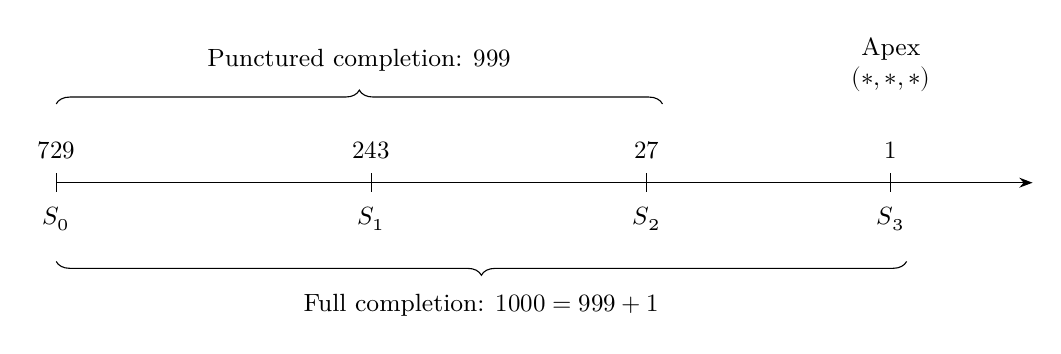
\begin{tikzpicture}[x=1cm,y=1cm,>=Stealth,font=\small]
\draw[->] (0,0)--(12.4,0);
\foreach \x/\a/\b in {0/729/{S_0},4.0/243/{S_1},7.5/27/{S_2},10.6/1/{S_3}}{
  \draw (\x,0.12)--(\x,-0.12);
  \node[above=5pt] at (\x,0) {\(\a\)};
  \node[below=5pt] at (\x,0) {\(\b\)};
}
\draw[decorate,decoration={brace,amplitude=5pt}] (0,1)--(7.7,1);
\node[above=8pt] at (3.85,1) {Punctured completion: \(999\)};
\draw[decorate,decoration={brace,mirror,amplitude=5pt}] (0,-1)--(10.8,-1);
\node[below=8pt] at (5.4,-1) {Full completion: \(1000=999+1\)};
\node[align=center] at (10.6,1.5) {Apex\\\((\ast,\ast,\ast)\)};
\end{tikzpicture}
\caption{Strata of the cubic completion. The arrangement represents
the set-theoretic decomposition, not a metric scale. The \(243\) elements
of \(S_1\) form three coordinate strata of \(81\) elements; the \(27\)
elements of \(S_2\) form three strata of \(9\). The apex completes the partition.}
\label{fig:revision-emrh}
\end{figure}

% Geometric adaptation of the preserved cubic-completion figure.
\begin{figure}[htbp]
\centering
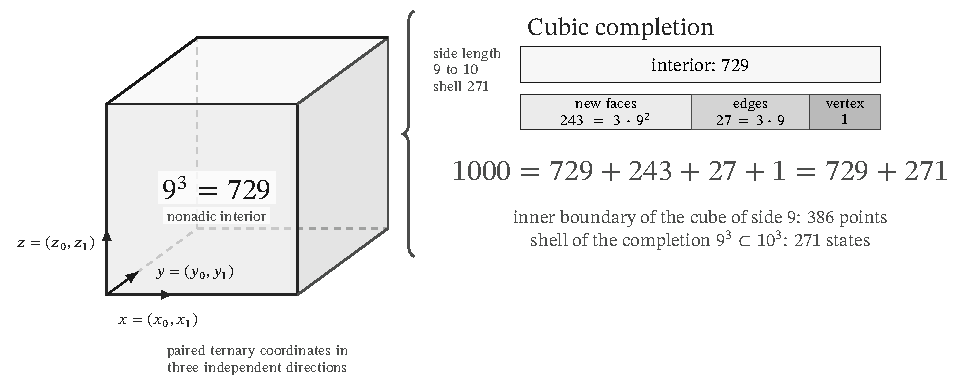
\includegraphics[width=\linewidth]{figures/cubo_emrh.pdf}
\caption{Cubic representation of the expansion from nine to ten classes per coordinate. Strata \(S_1,S_2,S_3\) locate the added incidences on faces, edges, and the apex; their cardinalities form the \(271\)-element shell. The \(386\)-element boundary belongs to the initial cube. This geometric perspective complements the partition in Figure~\ref{fig:revision-emrh}; graphical spacing is schematic.}
\label{fig:completacion-cubo-recuperado}
\end{figure}


\subsubsection{Conservation of unity and dimensional compatibility}

Normalization is not limited to dividing an isolated identity. In dimension
\(d\), the product \(\widehat E^d\) carries the uniform measure
\(\mu_d(\{x\})=10^{-d}\). The coordinate projection
\(p_d:\widehat E^{d+1}\to\widehat E^d\) deletes the last coordinate.

\begin{proposition}[Projective compatibility of normalized measures]
For every \(d\geq1\),
\[
 (p_d)_*\mu_{d+1}=\mu_d,
 \qquad \mu_d(\widehat E^d)=1.
\]
The mass of the stratum with \(r\) additional coordinates is
\(\binom dr9^{d-r}/10^d\), and the masses of all strata sum to one.
\end{proposition}
\begin{proof}
Each point of \(\widehat E^d\) has ten preimages. Their total mass is
\(10\,10^{-(d+1)}=10^{-d}\). Equality for any subset follows by
summing over its points. The stratified formula follows from the same
count as \eqref{eq:revision-estratos}; the binomial
\((9+1)^d\) gives total normalization.
\end{proof}

In dimension three, removing the apex leaves mass \(999/1000\), and
restoring it adds \(1/1000\). Renormalizing before restoration would
define a different measure: the distinction is operationally relevant.
In particular, conservation of probability mass, conservation of transport
records, and thermodynamic dissipation concern different objects. The
proposition proves the first and provides the compatible support for
studying the second; the third requires a specified dynamic and energetic realization.

The internal geometric boundary also remains distinct.
On the Cartesian representative \(\{1,\ldots,9\}^3\), removing
\(\{2,\ldots,8\}^3\) leaves \(386\) points. This boundary belongs
to the initial cube, whereas \(\widehat C\setminus C\) belongs to
its expansion. Cubic completion, base-thousand positional expansion,
and exceptional-incidence reading share support data; their respective
maps determine which information from these data each representation uses.


\subsection{Cubic incidence and Lorentzian realization}

Cubic completion supplies a relation between interior and boundary.
Its geometry can be developed through incidence of the six faces with
the eight vertices. Label faces by \((i,\varepsilon)\),
\(i\in\{1,2,3\}\), \(\varepsilon\in\{+1,-1\}\), and vertices by
\(\nu\in\{+1,-1\}^3\). The incidence matrix is
\[
 M_{(i,\varepsilon),\nu}=\mathbf1_{\{\nu_i=\varepsilon\}}.
\]
Let \(u=(1,\ldots,1)^{\mathsf T}\in\RR^6\), let \(R_F\) denote
face opposition, and let \(P_u=uu^{\mathsf T}/6\), \(P_-=(I-R_F)/2\).

\begin{proposition}[Four-dimensional incidence quotient]
The incidence Gram matrix satisfies
\[
 MM^{\mathsf T}=12P_u+4P_-.
\]
Its eigenvalues \(12,4,0\) have multiplicities \(1,3,2\).
Consequently,
\[
 Q_\square=\RR^6/\ker(MM^{\mathsf T})
 \simeq\RR u\oplus E_-,\qquad E_-=\operatorname{im}P_-.
\]
\end{proposition}
\begin{proof}
A face contains four vertices; two opposite faces have empty intersection,
and two distinct non-opposite faces share two vertices.
The matrix \(12P_u+4P_-\) has exactly these entries.
The uniform subspace has dimension one; differences between opposite
faces generate a three-dimensional space orthogonal to it.
Its complement has dimension two and belongs to the kernel.
\end{proof}

The decomposition \(1+3\) comes from incidence. The temporal choice
is declared through the bilinear form
\[
 B_\square([x],[y])=\langle x,(P_--P_u)y\rangle.
\]
It is well defined on the quotient because both projectors annihilate
the kernel. In the basis
\[
 t=[u]/\sqrt6,\qquad
 d_i=[e_{i,+}-e_{i,-}]/\sqrt2,
\]
its matrix is \(\operatorname{diag}(-1,1,1,1)\). The domain,
decomposition, and sign convention producing the Minkowski realization
are thus explicit. The positive Gram matrix determines the quotient;
the temporal assignment determines the indefinite form on it.

The operator
\[
 W_\square=\sqrt6P_u+\sqrt2P_-,\qquad
 W_\square e_{i,\varepsilon}=t+\varepsilon d_i
\]
sends the six face labels to null directions, since
\(B_\square(t+\varepsilon d_i,t+\varepsilon d_i)=-1+1=0\).
Direction reversal and face opposition thus acquire a concrete
geometric realization.

\subsubsection{Soldering, reversal, and subdivision}

The cellular realization uses an invertible transport \(U_m(a)\),
preserving the Lorentzian form, between the endpoint fibers of an
oriented dual edge \(a\), a face label \(\lambda_m(a)\),
and an orientation \(\sigma_m(a)\).
With \(\ell_m=\ell_0/9^m\), the soldering map is
\[
 \beta_m(a)=\ell_m\sigma_m(a)
 W_{\square,s(a)}e_{\lambda_m(a)}.
\]
Compatible reversal satisfies
\[
 \beta_m(\bar a)=-U_m(a)\beta_m(a).
\]
Identify the source fibers at two consecutive levels through the declared
refinement isometry. If the nine subsegments \(a_1,\ldots,a_9\),
at level \(m+1\), preserve label and orientation when transported
to that common fiber, then
\begin{equation}
 \beta_m(a)=\sum_{j=1}^9
 U_{m+1}(a_1\cdots a_{j-1})^{-1}\beta_{m+1}(a_j).
 \label{eq:soldadura-refinamiento}
\end{equation}
Each transported term equals \(\ell_m/9\) times the same null
direction, proving the identity. The compatibility hypothesis determines
which subdivisions realize this refinement. The equation brings together
direction, scale, and transport, rather than limiting geometric
correspondence to a dimension count.

With orientation and the Lorentzian form also fixed, Hodge duality
on \(\Lambda^2Q_\square^*\) satisfies \(\star^2=-I\).
In dimension four, the sign is \((-1)^{2(4-2)+1}=-1\).
This yields a real complex structure on two-forms and, after
complexification, the eigenspaces with eigenvalues \(+i\) and \(-i\).
The electromagnetic realization will use this domain after constructing
the electronic section and declaring its coupling.

\subsection{Compatibility of modular and positional reductions}

The block-decimal base enters through Euclidean division preserving
residue and quotient simultaneously:
\[
 n=1000q+r,\qquad 0\le r<1000.
\]
Since \(1000\equiv1\pmod9\) and \(1000\equiv1\pmod3\),
\[
 n\equiv q+r\pmod9,\qquad n\equiv q+r\pmod3.
\]
Reduction of a block therefore requires the quotient's contribution
to recover the integer's class. The numbers \(0\) and \(1000\)
have the same remainder modulo \(1000\), but different classes
modulo \(9\) and \(3\). This is an operational reason for preserving
memory through a change of resolution.

Ternary refinement and determination of a decimal prefix can be
coordinated through a single integer remainder. If \(N/3^L\)
is a cylinder endpoint and \(D/1000^r\) a decimal endpoint, define
\[
 A=1000^rN-D3^L.
\]
On adding six ternary symbols, \(N'=729N+\nu\),
\(L'=L+6\), with \(0\le\nu<729\). If the decimal prefix remains
fixed, one obtains
\[
 A'=729A+\nu1000^r.
\]
If a decimal block \(\delta\) is also incorporated, then
\(D'=1000D+\delta\), \(r'=r+1\), and
\begin{equation}
 A'=729000A+\nu1000^{r+1}-729\delta3^L.
 \label{eq:residuo-dos-bases}
\end{equation}
Both identities follow by substitution of the definitions. Comparing
endpoints is thus reduced to integer operations retaining each
prolongation's contribution. This compatibility makes it possible
to refine a region before evaluating its real coordinate.

% Incorporation at the end of extension.tex; contains no main section.
% Provenance: RESULTADO_RECUPERADO; sector-specific explicit statement of hypotheses.
% Sources read: Doble proyección holográfica monograph (editorial source material),
% manuscrito/local/01_tesis_recuperada.tex and
% manuscrito/generated/algebra_holonomica.tex, especially §§1--7 and 21.
% Governing definition of number: manuscrito/flattened/main_autosuficiente.tex,
% sections starting at lines 22137 and 23000 of the 775-page source collection.
% Its global presentation is not adopted as proof of every TPK arrow.

\subsection{Number as a compatible section and value as a reading}
\label{hist:seccion}

Distinguishing state from observation specifies what object is prolonged
as resolution increases. At depth \(n\), let \(X_n\) be the set of
admissible states produced by APP--TRIT--TPK. Their data include position,
sum and product sheets, residues and quotients, regime, orientation,
carry, phase, route, boundary, memory, and survival. These are not
independent coordinates: earlier arithmetic evaluations and transports
impose their relations. A prolongation preserves these relations in
each antecedent, even while adding new steps and memory data.
This is the meaning of the arithmetic of histories formalized below.

Let \(r_{m,n}:X_m\to X_n\), for \(m\geq n\), be depth
restrictions, with \(r_{n,n}=\operatorname{id}\) and
\(r_{\ell,n}=r_{m,n}\circ r_{\ell,m}\). Each restriction preserves
the prefix and the information already determined in it.

\begin{definition}[Compatible numerical section]
An HMT number is a compatible history of the state system:
\begin{equation}
 x=(x_n)_{n\geq0}\in X_\infty:=\varprojlim_n X_n,
 \qquad r_{m,n}(x_m)=x_n.
 \label{hist:limite-inverso}
\end{equation}
A reader is an additional operation on a specified domain of these
histories. A digit is a finite observation; a scalar value is an evaluation
of the reader. The pair consisting of a section and its reader constitutes
a read presentation, not a redefinition of the section's identity.
\end{definition}

On the Archimedean domain \(X_\infty^{\mathrm{Arch}}\), the reader
associates a closed cylinder with each prefix, preserves nesting, and
makes its diameter tend to zero. It thus determines
\begin{equation}
 \operatorname{ev}_{\mathbb R}:X_\infty^{\mathrm{Arch}}\longrightarrow
 \mathbb R,\qquad
 \{\operatorname{ev}_{\mathbb R}(x)\}=\bigcap_n I_n(x).
 \label{hist:evaluacion}
\end{equation}
The concrete construction of these cylinders and the determination of
their boundaries are developed in Section~\ref{sec:generacion}.
Definition \eqref{hist:limite-inverso} does not by itself assert
that the image of \eqref{hist:evaluacion} is the entire line:
a coverage claim requires its own theorem. Nor does equality of
values establish equality of histories without an injectivity result.
This separation allows precision to be discussed as depth while preserving
the distinction between the arithmetic antecedent and its scalar realization.

\subsection{Composition of histories and memory multiplier}
\label{hist:algebra}

Fix a sector of states at depth \(n\) and a category \(\mathcal C\)
whose arrows are its admissible histories. Composition is written
\(vu=v\circ u\): first traverse \(u\), then \(v\).
Elementary steps come from TPK selection, transport, and updating.
A local tritic fiber admits the notation
\(\mathbb R[J_x]/(J_x^2+\tau(x)1_x)\), where
\(\tau(x)\in\{+1,0,-1\}\). Regime and orientation belong to
the transported state; a transition between regimes does not amount
to identifying their quadratic algebras.

The following formulation specifies an algebraic sector of this composition.
For each object \(x\), a unital associative real algebra \(A_x\),
possibly noncommutative, is given. For each \(u:x\to y\), a
unital homomorphism \(\rho_u:A_x\to A_y\) is given. Assume a strict action:
\begin{equation}
 \rho_{\operatorname{id}_x}=\operatorname{id}_{A_x},\qquad
 \rho_v\rho_u=\rho_{vu}.
 \label{hist:accion-estricta}
\end{equation}
For each composable pair \(u:x\to y\), \(v:y\to z\), fix an
invertible central multiplier \(\Omega(v,u)\in Z(A_z)^\times\).
Require the normalization
\(\Omega(\operatorname{id}_y,u)=\Omega(u,\operatorname{id}_x)=1_y\)
and, for every composable triple, the identity
\begin{equation}
 \rho_w\bigl(\Omega(v,u)\bigr)\Omega(w,vu)
   =\Omega(w,v)\Omega(wv,u).
 \label{hist:cociclo}
\end{equation}
These are explicit hypotheses on transports and their coefficients,
not a consequence of calling the dynamics holonomic. Applying this
presentation to a TPK sector requires identifying its \(\rho_u\)
and \(\Omega(v,u)\). Transitions expressed through bimodules require
preserving that structure and are not replaced by \eqref{hist:accion-estricta}.

The space of finite sums
\[
 \mathcal H(\mathcal C,A,\rho,\Omega)
   =\bigoplus_{u\in\operatorname{Mor}(\mathcal C)} A_{t(u)}T_u
\]
receives the bilinear product
\begin{equation}
 (aT_v)(bT_u)=a\rho_v(b)\Omega(v,u)T_{vu},
 \label{hist:producto}
\end{equation}
when the arrows are composable, and zero otherwise. Here \(t(u)\)
denotes the terminal state. Addition gathers histories with coefficients;
multiplication concatenates histories while preserving the record multiplier.

\begin{proposition}[Sectorial associativity with a central multiplier]
Under \eqref{hist:accion-estricta} and \eqref{hist:cociclo}, product
\eqref{hist:producto} is associative. If the object set is finite,
its identity is \(\sum_x1_xT_{\operatorname{id}_x}\).
\end{proposition}
\begin{proof}
For \(u:x\to y\), \(v:y\to z\), \(w:z\to t\), let
\(a\in A_y\), \(b\in A_z\), \(c\in A_t\). The two coefficients
of \(T_{wvu}\) are
\begin{align*}
 ((cT_w)(bT_v))(aT_u):\quad&
 c\rho_w(b)\Omega(w,v)\rho_{wv}(a)\Omega(wv,u),\\
 (cT_w)((bT_v)(aT_u)):\quad&
 c\rho_w(b)\rho_w\rho_v(a)\rho_w(\Omega(v,u))\Omega(w,vu).
\end{align*}
The strict action identifies \(\rho_w\rho_v(a)\) with \(\rho_{wv}(a)\).
Centrality of \(\Omega(w,v)\) allows it to move to the right of
that factor; \eqref{hist:cociclo} then equates the remaining products.
The coefficients \(a,b,c\) are not permuted. If the triple is not
composable, both parenthesizations are zero because of their initial
and terminal states. Bilinearity completes the proof. Local identities
and normalization of \(\Omega\) verify the stated identity element.
\end{proof}

Calendar carry provides an effective example. In the category with one
object and arrows \(C_9\), take coefficients
\(A=\mathbb R[z,z^{-1}]\), the identity action, and
\[
 \Omega(b,a)=z^{c_0(a,b)},\qquad
 c_0(a,b)=\left\lfloor\frac{a+b}{9}\right\rfloor,
 \quad 0\leq a,b<9.
\]
The two carry sums of a triple are
\(\lfloor(a+b+c)/9\rfloor\); hence \eqref{hist:cociclo} holds.
The formal variable \(z\) records the turn without assigning it a
numerical value. Subsequently imposing \(z^{12}=1\) recovers the
dodecaphase record of calendar \eqref{eq:extension108}; retaining
\(z\) without that relation distinguishes successive turns. The example
realizes this calendar's memory without identifying it with all TPK memory.

\subsection{Double variance of refinement and conservation of unity}
\label{hist:doble-varianza}

Restricting states prolongs observables in the opposite direction.
Consider the function algebras, with pointwise product,
\(D_n=\operatorname{Fun}(X_n,\mathbb R)\). Precomposition defines
\begin{equation}
 r_{m,n}^*:D_n\longrightarrow D_m,
 \qquad r_{m,n}^*f=f\circ r_{m,n}.
 \label{hist:precomposicion}
\end{equation}
These are unital morphisms; they are also injective when the corresponding
restrictions are surjective. The direct limit
\(D_{\mathrm{cyl}}=\varinjlim_n(D_n,r_{n+1,n}^*)\) gathers
finite-depth observations. This algebra is not identified here with
the whole route algebra: prolonging transport operators also requires
their compatibility with refinement.

\begin{lemma}[Identity and naturality of evaluation]
If \(e_x\) is the indicator of \(x\in X_n\), then
\begin{equation}
 r_{m,n}^*e_x=\sum_{y:\,r_{m,n}(y)=x}e_y,
 \qquad r_{m,n}^*1_n=1_m,
 \label{hist:unidad}
\end{equation}
and, for every \(f\in D_n\), \(y\in X_m\),
\[
 \langle r_{m,n}^*f,y\rangle=\langle f,r_{m,n}y\rangle.
\]
Each section \(x\in X_\infty\) determines a well-defined evaluation
\(D_{\mathrm{cyl}}\to\mathbb R\), given by \([f]\mapsto f(x_n)\)
for \(f\in D_n\).
\end{lemma}
\begin{proof}
The fibers of \(r_{m,n}\) partition \(X_m\). Their indicators
are orthogonal and sum to \(1_m\), proving \eqref{hist:unidad}.
Naturality is the definition of precomposition. Finally,
\((r_{m,n}^*f)(x_m)=f(x_n)\), so two compatible representatives
give the same evaluation in the direct limit.
\end{proof}

The global identity is the constant function one on all possibilities;
an individual section selects a compatible history. Preserving the former
does not mean immobilizing the latter. Refinement may increase the number
of extensions and the depth of each history while preserving the identity
and all evaluations of its antecedents.

\subsection{Phase return, Weyl representation, and two readings}
\label{hist:puente-lecturas}

Law \eqref{eq:holonomia-memoria} acquires an operator realization
in the bilateral suspension constructed in Section~\ref{sec:generacion}.
There, \(T\) is one-step advance, \(V_9\) observes the nonadic phase,
\(W_\delta\) the rotation phase, and \(D_M\) the memory degree.
Writing \(\widehat\Gamma_9=T^9\) for the turn in this representation,
the Weyl relations \eqref{eq:weyl-relojes} imply, on finitely
supported vectors,
\begin{equation}
 \begin{aligned}
 V_9\widehat\Gamma_9&=\widehat\Gamma_9V_9,\qquad
 W_\delta\widehat\Gamma_9=e^{2\pi i9\delta}
     \widehat\Gamma_9W_\delta,\\
 [D_M,\widehat\Gamma_9]&=\widehat\Gamma_9.
 \end{aligned}
 \label{hist:tres-retornos}
\end{equation}
The first equality follows from \(\zeta_9^9=1\); the second from
nine applications of the covariance of \(W_\delta\); the third
expresses the unit memory increment. The finite phase returns while
irrational rotation and memory distinguish the next state. Characters
and parameter \(\delta\) are realized subsequently from the numerical
construction specified there: they do not select the seeds retrospectively.
This representation describes suspension observables and translations;
it does not replace all TPK coordinates or operators.

The double reading extends the same distinction between history and observable.
On its Archimedean domain, \eqref{hist:evaluacion} applies; on the
calibrated incidence domain, the maps \(Q_n\) of
Section~\ref{exc:doble-lectura} preserve words and boundary frames.
The equality proved there,
\(r_{n,m}Q_n=Q_mp_{n,m}\), determines their prolongation \(Q_\infty\).
On the common domain of both readings,
\(\operatorname{ev}_{\mathbb R}(x)\) and \(Q_\infty(x)\)
can be considered jointly: the former retains the value; the latter,
the transported incidence preserved by its codomain. The section
precedes both. This articulation makes it possible to pass from the
arithmetic of histories to constants and exceptional reading without
turning their realizations into new initial data.


\clearpage
\section{Coinductive generation of \texorpdfstring{\(\pi,\varphi,e\)}{pi, phi, e} to arbitrary depth}
\label{sec:generacion}

The six-block emission is a finite stage of the construction, not a complete decimal expansion. Its function is to produce regions with multiplicity, orientation, and transport rules. Prolongation must preserve these data and determine a compatible collection of prefixes of arbitrary length. The word \emph{generation} designates this operation; \emph{genealogy} designates the reconstruction of its dependencies. Both notions enter the discussion, but perform distinct functions.

\subsection{Orbits, regions, and characters of closure, propagation, and self-scaling}

On a word \(w=(w_1,\ldots,w_6)\), we define
\[
 r(w)=(w_3,w_1,w_2,w_5,w_6,w_4),\qquad
 s(w)=(w_4,w_5,w_6,w_1,w_2,w_3).
\]
We have \(r^3=s^2=I\) and \(srs=r^{-1}\); these permutations therefore realize the dihedral group \(D_3\). The action preserves the catalog and multiplicities and commutes with \(\Psi\). The quotient of the \(243\) visible words has \(43\) orbits: thirty-eight of cardinality six and five of cardinality three.

The closure class is recognized by a fiber predicate: its six orientations have five emissions per word, total multiplicity \(1008\), and distribution \(432+4\cdot144\). There is a single orbit with these properties in the catalog. To specify the other two selections, we write \(f(w)=\#\Psi^{-1}(w)\), \(m(w)=\sum_{U\in\Psi^{-1}(w)}\operatorname{mult}(U)\), and \(\nu(w)=(n_0,n_1,n_2)\). The additive diagonal class of an emission is \(d(U)=[i+j]_9\) in indices from zero to eight; its additive signature preserves this class and the orientation \(ES\) or \(NO\). Let \(\mathcal D(\mathcal O)\) be the set of these classes for all emissions over an orbit.

Among the orbits of size six, the joint predicate
\[
 f(w)=1,\qquad m(w)=144\quad(w\in\mathcal O),\qquad
 \mathcal D(\mathcal O)=\{0,3,6\}
\]
leaves exactly six orbits. In this sector, the census \(\nu=(2,3,1)\), equal to that of closure, selects propagation uniquely; the census \(\nu=(2,2,2)\) selects self-scaling uniquely. The diagonal support cannot be omitted: without it there are four balanced singleton-fiber orbits of multiplicity \(144\), not one. Finally, the existence of an emission with \(d=6\) and orientation \(ES\) selects a representative of each orbit and leads to
\begin{equation}
 w^{\rm cl}=010211,\qquad w^{\rm pr}=201101,\qquad w^{\rm au}=121200.
 \label{eq:palabras-regionales}
\end{equation}
These symbols first designate regions of the catalog. Scalar identification will be proved through their readers; they are not chosen because they coincide with digits of a known constant.

The closure word \(010211\) has the following five preimages:
\begin{center}\small
\begin{tabular}{@{}lll r@{}}\toprule
Six-block emission&Multiplicative signature&Role&Multiplicity\\\midrule
\(501,614,498,169,272,272\)&\(555555\)&transversal&432\\
\(810,923,870,169,272,272\)&\(339555\)&positive orientation&144\\
\(810,983,810,169,272,272\)&\(393555\)&positive orientation&144\\
\(870,923,810,169,272,272\)&\(933555\)&positive orientation&144\\
\(870,923,810,418,674,521\)&\(933717\)&oriented return&144\\\bottomrule
\end{tabular}
\end{center}
The multiplicity \(432\) and constant signature \(555555\) characterize the transversal region. They do not identify the central position \((5,5)\) of APP. Confusing a six-window signature with a position of the support would eliminate the distinction between numerical region and electronic structure.

The microfiber also has a precise bipartite morphology. Each emission is a product of an additive-cursor class and a multiplicative class. The three positive regions share the same additive class of eighteen conditions; together they contain three multiplicative classes of eight conditions each. The transversal region has a product \(18\times24\); the three positive regions together, another \(18\times24\); and the return, a product \(18\times8\). The decomposition by emissions has five parts, whereas the decomposition by connected components of the bipartite graph has three. Both preserve the same \(1008\) seeds without reducing form to a cardinality.

% BEGIN R27_REG01
\subsection{Incidences between halves of regional emissions}
\label{sec:rec27-empalmes}

Let $\mathcal U_6$ be the image of six consecutive windows of the emitter
of Section~\ref{act21:tpk:emision}. For $u=(u_1,\ldots,u_6)$, define
$A(u)=(u_1,u_2,u_3)$ and $B(u)=(u_4,u_5,u_6)$.
The half-emission graph has these triples as vertices and an undirected
edge between $A(u)$ and $B(u)$ for each emission.

\begin{proposition}[Cycle of regional junctions]
The vertices
\[
\begin{aligned}
A&=(830,943,830),&B&=(109,252,252),\\
C&=(810,923,870),&D&=(169,272,272),\\
E&=(850,963,890),&F&=(149,252,212)
\end{aligned}
\]
form the cycle $A-B-C-D-E-F-A$.
\end{proposition}
\begin{proof}
Write each seed as $(i,j,d)$, with residual positions between $0$ and $8$
and directions $N=(-1,0)$, $E=(0,1)$ and $S=(1,0)$.
Under the 54-step recurrence, the following seed pairs produce the six
emissions shown:
\[
\begin{array}{c|c|c}
\text{emission}&s_+&s_\times\\\hline
A\mid B&(0,6,E)&(0,6,N)\\
B\mid C&(0,6,N)&(1,5,E)\\
C\mid D&(0,6,E)&(0,1,S)\\
D\mid E&(0,6,N)&(0,4,S)\\
E\mid F&(0,6,E)&(0,3,E)\\
F\mid A&(0,6,N)&(0,1,S)
\end{array}
\]
Each row witnesses membership in $\mathcal U_6$ by successive evaluation
of the two accumulators. Splitting each emission into its two halves yields
exactly the six edges of the cycle.
\end{proof}

In the classification \eqref{eq:palabras-regionales},
\(A\mid B\), \(C\mid D\) and \(E\mid F\) respectively produce
the words \(w^{\rm au}\), \(w^{\rm cl}\) and \(w^{\rm pr}\).
The regional readers subsequently identify these outputs with
\(\varphi\), one region of \(\pi\) and \(e\).
The other three emissions exhibit their junctions in the graph.
The result describes incidences between emitter outputs. Temporal
realization of an incidence additionally uses the orientation, phase and
memory of the enriched state. Including the APP anchor and all five regions
of $\pi$ imposes further path conditions; the cycle above retains its role
as a local junction witness.

The six-edge cycle belongs to this undirected half-emission graph.
An enriched temporal path additionally retains the anchoring, orientation
and closure data of its construction. Incidence between two halves and
transport of a state thus have explicit domains and composition
conditions.

% END R27_REG01

% BEGIN R28_REGIONAL_CLOSURES_INPUT
% BEGIN R28_REGIONAL_CLOSURES
% Insert after REG01. This is not a standalone document.
% Provenance: U012_biografia_estructural_pi.tex, lines 175--324.
% Oriented witnesses: verificar_cierres_regionales.py; same problem,
% representatives different from the walks printed in U012.
% Emitter SHA-256: 42fdacab582de8e2d2cb7dfafc6204d200aef01249b3dcc37949e39507f066d8.
\subsubsection{Block multigraph and five minimal regional closures}
\label{regcl27:seccion}

The \(468\) emissions in \(\mathcal U_6\), produced by the
APP--TRIT--TPK emitter, determine a block multigraph. Identifying its
regional anchors makes it possible to solve a joint edge-covering
problem: to traverse the APP, propagation, autoscale, and each closure
region's incidences within a single closed walk. The local six-junction
cycle of Section~\ref{sec:rec27-empalmes} and these covers retain their
respective traversal conditions.

\paragraph{Block graph and exact phase quotient.}
For \(U=(U_1,\ldots,U_6)\in\mathcal U_6\), define
\begin{equation}
 A(U)=(U_1,U_2,U_3),\qquad B(U)=(U_4,U_5,U_6).
 \label{regcl27:mitades}
\end{equation}
The undirected multigraph \(\widetilde G\) has as vertices the triples
occurring as \(A(U)\) or \(B(U)\), and one edge labelled by each \(U\),
incident at those two triples. All \(468\) labels are retained:
distinct emissions are not identified merely because they share
endpoints or because one interchanges the halves of another.

Internal phase acts on each triple by cyclic rotation:
\begin{equation}
 (a,b,c)\sim(b,c,a)\sim(c,a,b),\qquad
 \operatorname{can}(a,b,c)
 =\min_{\rm lex}\{(a,b,c),(b,c,a),(c,a,b)\}.
 \label{regcl27:fase}
\end{equation}
The graph \(G\) replaces the endpoints of edge \(U\) by
\(\operatorname{can}A(U)\) and \(\operatorname{can}B(U)\), retaining
its label. The equivalence acts precisely by the three cyclic rotations
of each vertex; every emission retains its identity as an edge.

Enumeration from the same emitter and component searches give
\begin{equation}
\begin{array}{c|r|l}
 & |V|&\text{component sizes}\\ \hline
 \widetilde G&96&(28,28,28,4,4,4)\\
 G&32&(28,4)
\end{array}
\label{regcl27:componentes}
\end{equation}
These data are obtained by collecting distinct endpoints, adding each
incidence in both directions, and traversing each unvisited component
by breadth-first search. Adjacency may be deduplicated when counting
components, but parallel labels are retained when searching for
closures with prescribed edges.

\paragraph{APP anchor and regional numbering.}
The three common edges are
\begin{equation}
\begin{aligned}
 U_{\rm APP}&=903|850|850|252|109|252,\\
 U_e&=850|963|890|149|252|212,\\
 U_\varphi&=830|943|830|109|252|252.
\end{aligned}
\label{regcl27:anclajes}
\end{equation}
Fix the endpoint
\(v_{\rm APP}=\operatorname{can}A(U_{\rm APP})=850|850|903\).
For the five already constructed regions, use the following order,
which places the transverse region in the fifth row:
\begin{equation}
\begin{array}{c|l|c|r}
 i&U_\pi^{(i)}&\rho_i&m_i\\ \hline
 1&810|923|870|169|272|272&++&144\\
 2&810|983|810|169|272|272&++&144\\
 3&870|923|810|169|272|272&++&144\\
 4&870|923|810|418|674|521&--&144\\
 5&501|614|498|169|272|272&\perp&432
\end{array}
\label{regcl27:regiones}
\end{equation}
This numbering distinguishes the three \(++\) regions, the mutated
return \( -- \), and the transverse region \(\perp\). Accordingly,
\(\rho=(++ ,++ ,++ ,--,\perp)\) and
\(m=(144,144,144,144,432)\) in this order; their sum remains \(1008\).

\paragraph{Five complete witnesses with traversal directions.}
In each table, row \(j\) means traversing the edge labelled \(e_j\)
from \(v_{j-1}\) to \(v_j\). Endpoints are canonical phase representatives;
since \(G\) is undirected, the pair \((v_{j-1},v_j)\) specifies
the traversal direction of the labelled edge.
Each table contains exactly eight edges and satisfies
\(v_0=v_8=v_{\rm APP}\).

The breadth-first search described in the proof yields the following
witnesses, one for each set of four target edges. Minimality concerns
length; several walks may attain that length.
\paragraph{Witness \(i=1\).}
\begin{center}
\small
\begin{tabular}{rlll}
\hline
\(j\)&\(v_{j-1}\)&\(e_j\)&\(v_j\)\\
\hline
1&\(850|850|903\)&\(109|252|252|850|903|850\)&\(109|252|252\)\\
2&\(109|252|252\)&\(109|252|252|810|923|870\)&\(810|923|870\)\\
3&\(810|923|870\)&\(810|923|870|169|272|272\)&\(169|272|272\)\\
4&\(169|272|272\)&\(169|272|272|850|963|890\)&\(850|963|890\)\\
5&\(850|963|890\)&\(850|963|890|149|252|212\)&\(149|252|212\)\\
6&\(149|252|212\)&\(149|252|212|830|943|830\)&\(830|830|943\)\\
7&\(830|830|943\)&\(830|943|830|109|252|252\)&\(109|252|252\)\\
8&\(109|252|252\)&\(903|850|850|252|109|252\)&\(850|850|903\)\\
\hline
\end{tabular}
\end{center}

\paragraph{Witness \(i=2\).}
\begin{center}
\small
\begin{tabular}{rlll}
\hline
\(j\)&\(v_{j-1}\)&\(e_j\)&\(v_j\)\\
\hline
1&\(850|850|903\)&\(169|272|272|850|903|850\)&\(169|272|272\)\\
2&\(169|272|272\)&\(169|272|272|810|983|810\)&\(810|810|983\)\\
3&\(810|810|983\)&\(810|983|810|169|272|272\)&\(169|272|272\)\\
4&\(169|272|272\)&\(169|272|272|850|963|890\)&\(850|963|890\)\\
5&\(850|963|890\)&\(850|963|890|149|252|212\)&\(149|252|212\)\\
6&\(149|252|212\)&\(149|252|212|830|943|830\)&\(830|830|943\)\\
7&\(830|830|943\)&\(830|943|830|109|252|252\)&\(109|252|252\)\\
8&\(109|252|252\)&\(903|850|850|252|109|252\)&\(850|850|903\)\\
\hline
\end{tabular}
\end{center}

\paragraph{Witness \(i=3\).}
\begin{center}
\small
\begin{tabular}{rlll}
\hline
\(j\)&\(v_{j-1}\)&\(e_j\)&\(v_j\)\\
\hline
1&\(850|850|903\)&\(169|272|272|850|903|850\)&\(169|272|272\)\\
2&\(169|272|272\)&\(169|272|272|850|963|890\)&\(850|963|890\)\\
3&\(850|963|890\)&\(850|963|890|149|252|212\)&\(149|252|212\)\\
4&\(149|252|212\)&\(149|252|212|870|923|810\)&\(810|870|923\)\\
5&\(810|870|923\)&\(870|923|810|169|272|272\)&\(169|272|272\)\\
6&\(169|272|272\)&\(169|272|272|830|943|830\)&\(830|830|943\)\\
7&\(830|830|943\)&\(830|943|830|109|252|252\)&\(109|252|252\)\\
8&\(109|252|252\)&\(903|850|850|252|109|252\)&\(850|850|903\)\\
\hline
\end{tabular}
\end{center}

\paragraph{Witness \(i=4\).}
\begin{center}
\small
\begin{tabular}{rlll}
\hline
\(j\)&\(v_{j-1}\)&\(e_j\)&\(v_j\)\\
\hline
1&\(850|850|903\)&\(169|272|272|850|903|850\)&\(169|272|272\)\\
2&\(169|272|272\)&\(169|272|272|850|963|890\)&\(850|963|890\)\\
3&\(850|963|890\)&\(850|963|890|149|252|212\)&\(149|252|212\)\\
4&\(149|252|212\)&\(149|252|212|870|923|810\)&\(810|870|923\)\\
5&\(810|870|923\)&\(870|923|810|418|674|521\)&\(418|674|521\)\\
6&\(418|674|521\)&\(418|674|521|830|943|830\)&\(830|830|943\)\\
7&\(830|830|943\)&\(830|943|830|109|252|252\)&\(109|252|252\)\\
8&\(109|252|252\)&\(903|850|850|252|109|252\)&\(850|850|903\)\\
\hline
\end{tabular}
\end{center}

\paragraph{Witness \(i=5\).}
\begin{center}
\small
\begin{tabular}{rlll}
\hline
\(j\)&\(v_{j-1}\)&\(e_j\)&\(v_j\)\\
\hline
1&\(850|850|903\)&\(109|252|252|850|903|850\)&\(109|252|252\)\\
2&\(109|252|252\)&\(109|252|252|501|614|498\)&\(498|501|614\)\\
3&\(498|501|614\)&\(501|614|498|169|272|272\)&\(169|272|272\)\\
4&\(169|272|272\)&\(169|272|272|850|963|890\)&\(850|963|890\)\\
5&\(850|963|890\)&\(850|963|890|149|252|212\)&\(149|252|212\)\\
6&\(149|252|212\)&\(149|252|212|830|943|830\)&\(830|830|943\)\\
7&\(830|830|943\)&\(830|943|830|109|252|252\)&\(109|252|252\)\\
8&\(109|252|252\)&\(903|850|850|252|109|252\)&\(850|850|903\)\\
\hline
\end{tabular}
\end{center}

\begin{theorem}[Minimality of the five regional edge covers]
\label{regcl27:minimalidad}
For each \(i\in\{1,\ldots,5\}\), among closed walks in \(G\)
traversing every edge of
\[
 E_i^*=\{U_{\rm APP},U_e,U_\varphi,U_\pi^{(i)}\}
\]
at least once, the minimum length, counting traversals with multiplicity,
is eight. Vertices and edges may be repeated.
\end{theorem}

\begin{proof}
Every closed walk traversing \(U_{\rm APP}\) passes through
\(v_{\rm APP}\). Cyclic rotation of its step list allows it to start at
that vertex without changing length or coverage. It therefore suffices
to solve the problem with a fixed starting vertex.

The search space is the finite set
\[
 \mathscr S_i=V(G)\times\mathcal P(E_i^*),
 \qquad |\mathscr S_i|\le32\cdot16=512.
\]
The initial state is \(s_0=(v_{\rm APP},\varnothing)\), and the terminal
state is \(s_*=(v_{\rm APP},E_i^*)\). Traversing an edge \(e\)
incident at \(v\) towards its other endpoint \(v'\) updates the state by
\begin{equation}
 (v,M)\longmapsto\bigl(v',M\cup(E_i^*\cap\{e\})\bigr).
 \label{regcl27:transicion-bfs}
\end{equation}
The mask records edge labels, not just endpoints; distinct parallel
edges must therefore not be collapsed.

Every transition has unit cost. A FIFO queue initialized at \(s_0\)
extracts states in increasing distance, marks each state on its first
visit, and stores its predecessor and traversed label.
Equivalently, with \(\mathcal F_0=\{s_0\}\), the new layers are
\[
 \mathcal F_{k+1}
 =\operatorname{Succ}(\mathcal F_k)
   \setminus\bigcup_{j=0}^{k}\mathcal F_j.
\]
Induction shows that \(\mathcal F_k\) contains exactly the states whose
minimum distance from \(s_0\) is \(k\). Finite enumeration over the
specified emitter gives, for each of the five regions,
\[
 s_*\notin\bigcup_{k=0}^{7}\mathcal F_k,\qquad s_*\in\mathcal F_8,
 \qquad (\ell_1,\ell_2,\ell_3,\ell_4,\ell_5)=(8,8,8,8,8).
\]
The tables exhibit the five upper bounds, including all four required
labels in each case. Exhaustive exploration of the preceding layers
proves the lower bound. Together they establish minimality for the
declared problem.
\end{proof}

Length eight characterizes the joint coverage of four incidences in
each closure region. The quotient retains emission labels and their
junctions between phase classes; enriched temporal evolution also
preserves orientation and memory. This description links all five
regions to the same propagation, autoscale, and APP anchors and
complements the local six-junction cycle. Coinductive prolongation
retains its operators and cylinders together with these orientation
and memory data.
% END R28_REGIONAL_CLOSURES

% END R28_REGIONAL_CLOSURES_INPUT

\subsection{Finite transport and the prolongation boundary}

The endomorphisms \(L_0,L_1\) of the ternary-word space act before Archimedean realization. Their determination begins with transitions of the arithmetic state, not with the prescription of two matrices. If \(U_t\) is the composite step of selection, transport, and updating, the observed block satisfies
\[
 b_j^\chi=\Pi_6(x_j^\chi),\qquad
 x_{j+1}^\chi=U_{9j+9}\cdots U_{9j+1}(x_j^\chi),
 \qquad \chi\in\{\mathrm{cl},\mathrm{pr},\mathrm{au}\}.
\]
Six transitions are formed for each regime: two consecutive transitions in each of the three regions. The pairs of source and target matrices obtained in the record are
\[
\begin{array}{c|c|c|c}
X_0&Y_0&X_1&Y_1\\\hline
010211&012222&010211&002111\\
012222&010211&002111&110221\\
201101&121221&102011&012222\\
121221&102011&012222&102011\\
121200&112202&121020&010210\\
112202&121020&010210&010200
\end{array}
\]
Each six-digit string represents a row in \(\FF_3^6\). Since \(\det X_0=1\) and \(\det X_1=-1\) in \(\FF_3\), the equations \(X_aL_a=Y_a\) uniquely determine \(L_a=X_a^{-1}Y_a\). In that row-vector chart, the result is
\[
 L_0=\begin{pmatrix}
 2&2&2&1&2&1\\2&1&2&2&1&1\\1&0&0&1&0&2\\
 0&0&1&1&1&0\\2&2&2&0&2&1\\2&1&2&1&0&0
 \end{pmatrix},\quad
 L_1=\begin{pmatrix}
 2&1&2&0&2&2\\1&2&1&1&2&0\\1&2&1&1&1&2\\
 0&1&0&0&2&1\\2&0&2&1&0&1\\0&2&2&2&1&1
 \end{pmatrix}\quad(\bmod3).
\]
The calendar \((L_0,L_0,L_1,L_1)\) produces four new blocks of six components. Their concatenations form
\[
 w_6\longrightarrow w_{12}\longrightarrow w_{18}
 \longrightarrow w_{24}\longrightarrow w_{30}.
\]
The subscripts of \(w\) indicate accumulated length. The boundary \(R_{36}\) preserves the terminal structure and opens the prolongation relation; it is not renamed as a final periodic block that could be repeated indefinitely.

The identity \(L=X^{-1}Y\) proves uniqueness once the transitions have been fixed; it does not replace the production of those transitions by \(U_t\). The provenance of their record and the examination of the sixteen binary calendars are documented in the technical supplement. The indicated calendar is the only one of those sixteen that jointly reproduces the three sequences of five blocks.

\subsection{Correlated construction and ordering of the readers}
\label{gen:orden-constructor-correlacionado}

The common antecedent of the three regions is the arithmetic emission
with its trajectory record. APP provides the sum and product evaluations;
TRIT provides the oriented signature; transition \eqref{eq:actualizacion}
composes mode selection, cardinal transport, and memory update. The
census of that emission produces the catalogue and its fibres. The
multiplicity, diagonal-support, and orientation predicates select the
representatives in \eqref{eq:palabras-regionales}. Regional correlation
preserves this joint provenance, together with the incidences and
restrictions between its records.

The transports \(L_0,L_1\) act on the selected representatives in the
declared row chart. The calendar and concatenation distinguish prefix
length, visible phase, and accumulated memory. The deep coordinate and
its quotients are made explicit below through
\eqref{memprof:division} and \eqref{memprof:inversa}. Restrictions of
histories are preserved in the sense of \ref{hist:seccion}. The concrete
oriented selection of \(R_{36}\) has its incidence proof in
\ref{mg01:frontera}, after the construction of \(A_W\); that placement
preserves the antecedents used by its proof.

Each regional reader adds a typed operation to the record it receives.
For closure, the symmetric reader of the pentafibre fixes the primitive
slope, and the composition law determines the compensator in
\eqref{eq:lector-pi}. For propagation, formal composition, the unit,
and the oriented generator determine recurrence \eqref{eq:propagacion}.
For autoscaling, the mode calendar produces incidence \eqref{eq:fav},
whose positive ray fixes the normalized coordinate. The following proofs
retain the normalizations and domains of these three operations.

Rational bounds and cylinder separation subsequently evaluate the
resulting characters. Effective positional emission and its
compatibility are proved in \ref{act21:thm:df-emision-correcta} and
\ref{act21:prop:df-prefijos-compatibles}. The dodecaphasic register
retains its own construction in \ref{act21:chap:despliegue-selector-k};
its coordinates and the three regional readings subsequently enter the
integer closure in \ref{sec:alpha}. Thus regional selection, transport,
character construction, and prefix evaluation retain their domains and
order within the same APP--TRIT--TPK genealogy.


\subsection{Deep memory and compatibility of the cylinders}
\label{memprof:seccion}

Prolongation compares states that simultaneously retain residues,
quotients, and boundaries. In the six-coordinate linear chart of the
record, take the integer representative of \(L_0\) whose entries were
displayed above:
\[
 A_H=\begin{pmatrix}
 2&2&2&1&2&1\\2&1&2&2&1&1\\1&0&0&1&0&2\\
 0&0&1&1&1&0\\2&2&2&0&2&1\\2&1&2&1&0&0
 \end{pmatrix},\qquad\det A_H=1.
\]
The choice of this representative is part of the chart: reduction modulo
three retains \(L_0\), whereas the integer representative fixes the
operation on the deep quotients. With row vectors, this gives
\begin{equation}
 \begin{aligned}
 \mathsf{Div}_H:\mathbb Z^6&\longrightarrow
       \{0,1,2\}^6\times\mathbb Z^6,\\
 x_H&\longmapsto(u_H,x_H^+),\\
 y_H&=x_HA_H,\qquad u_H=[y_H]_3,\qquad
 x_H^+=(y_H-u_H)/3 .
 \end{aligned}
 \label{memprof:division}
\end{equation}
The pair \((u_H,x_H^+)\) retains \(y_H=u_H+3x_H^+\). Since
\(A_H\) is unimodular, its inverse has integer entries and
\begin{equation}
 x_H=(u_H+3x_H^+)A_H^{-1}.
 \label{memprof:inversa}
\end{equation}
This identity recovers the deep coordinate from its residue and quotient.
The other state fields retain their own records. The ternary orientation
is subsequently read through
\(0\mapsto0,\ 1\mapsto+1,\ 2\mapsto-1\), retaining the residue
\(u_H\in\{0,1,2\}^6\) and the quotient in \eqref{memprof:division}.

The cylinder chart relates a ternary prefix of length \(L\), with integer
index \(N\), to \(k_{\mathrm{dec}}\) decimal triads, with index \(D\).
The corresponding half-open cylinders are
\[
 I_3(N,L)=\left[\frac N{3^L},\frac{N+1}{3^L}\right),\qquad
 I_{1000}(D,k_{\mathrm{dec}})
 =\left[\frac D{1000^{k_{\mathrm{dec}}}},
         \frac{D+1}{1000^{k_{\mathrm{dec}}}}\right).
\]
Define the boundary integers
\[
 a_{\mathrm{cyl}}=N1000^{k_{\mathrm{dec}}}-D3^L,\qquad
 b_{\mathrm{cyl}}=(N+1)1000^{k_{\mathrm{dec}}}-D3^L.
\]
For a block of six residues, fix its integer encoding as
\[
 \nu(u_H)=\sum_{j=1}^6(u_H)_j3^{6-j}
 \in\{0,\ldots,728\}.
\]

\begin{lemma}[Integer update of compatible cylinders]
\label{memprof:cilindros}
The preceding cylinders intersect if and only if
\(a_{\mathrm{cyl}}<3^L\) and \(b_{\mathrm{cyl}}>0\).
Appending a ternary block with index
\(\nu\in\{0,\ldots,728\}\) gives \(N'=729N+\nu\) and
\(L'=L+6\). For \(\Delta k_{\mathrm{dec}}\in\{0,1\}\),
the boundaries update according to
\[
 \begin{array}{ll}
 \Delta k_{\mathrm{dec}}=0:
   &a_{\mathrm{cyl}}'=729a_{\mathrm{cyl}}+\nu1000^{k_{\mathrm{dec}}},\\[2pt]
 \Delta k_{\mathrm{dec}}=1:
   &D'=1000D+\delta,\\
   &a_{\mathrm{cyl}}'=729000a_{\mathrm{cyl}}
      +\nu1000^{k_{\mathrm{dec}}+1}-\delta\,729\,3^L ,
 \end{array}
\]
where \(\delta\in\{0,\ldots,999\}\) is the triad of the compatible
prolongation. In both cases,
\[
 b_{\mathrm{cyl}}'=a_{\mathrm{cyl}}'
          +1000^{k_{\mathrm{dec}}+\Delta k_{\mathrm{dec}}}.
\]
\end{lemma}
\begin{proof}
Two half-open intervals intersect precisely when each left endpoint is
smaller than the right endpoint of the other interval. Multiplication
of these two inequalities by \(3^L1000^{k_{\mathrm{dec}}}\) gives
\(a_{\mathrm{cyl}}<3^L\) and \(b_{\mathrm{cyl}}>0\).
Substitution of \(N'\), \(L'\), and \(D'\) into
\[
 a_{\mathrm{cyl}}'
 =N'1000^{k_{\mathrm{dec}}+\Delta k_{\mathrm{dec}}}-D'3^{L'}
\]
gives the two recurrences. Subtracting the definitions of
\(b_{\mathrm{cyl}}'\) and \(a_{\mathrm{cyl}}'\) yields the final identity.
\end{proof}

These operations act on integer prefixes and their compatible
restrictions. The Archimedean reading appears when the resulting system
of cylinders is evaluated. The prolongation domain also incorporates
orientation, carry, the joint signature, and the boundary data of the state
\(\widehat X\) in \eqref{eq:actualizacion}; interval comparison is one
component of this joint compatibility.


\subsection{Five closure regions and angular compensation}

The closure region contains a transversal component and four companions. The symmetric reader acts on the space of its five positions through
\[
 P_5=\frac15\mathbf1\mathbf1^{\mathsf T},\qquad
 \mathbf1=(1,1,1,1,1)^{\mathsf T}.
\]
The invariance \(P_5\lambda=\lambda\) and conservation \(\mathbf1^{\mathsf T}\lambda=1\) force \(\lambda=\mathbf1/5\). This normalization distributes unity among reader positions; it does not replace the seed multiplicities \(432,144,144,144,144\) by uniform frequencies. The reader's elliptic chart realizes each coordinate through \(1+\lambda_jJ\); its slope is \(\lambda_j\), so the primitive slope is \(1/5\). This makes explicit the rule passing from a normalized coordinate to a slope, instead of identifying the two notions without a map. The reader composes the four companion positions by the law
\begin{equation}
 a\oplus b=\frac{a+b}{1-ab}.
 \label{eq:suma-pendientes}
\end{equation}
This law is obtained by multiplying \((1+aJ)(1+bJ)\) in the regime \(J^2=-I\) and dividing by its scalar component. Slope composition is therefore a realization of the quadratic structure of TRIT, not an ordinary sum of four fractions.

\begin{proposition}[Closure compensator]
The composition of four slopes \(1/5\) is \(120/119\). The condition of return to slope one determines a unique positive compensator of the form \(1/q\), with \(q>1\), and gives \(q=239\).
\end{proposition}
\begin{proof}
The first doubling gives \((1/5)\oplus(1/5)=5/12\); the second gives \((5/12)\oplus(5/12)=120/119\). The condition
\[
 \frac{120/119-1/q}{1+(120/119)/q}=1
\]
is equivalent to \((120-119)q=120+119\), hence \(q=239\).
\end{proof}

The resulting closure character has realization
\begin{equation}
 \Pi_{\rm cl}=4\left(4\arctan\frac15-\arctan\frac1{239}\right).
 \label{eq:lector-pi}
\end{equation}
Machin's angular identity recognizes \(\Pi_{\rm cl}=\pi\). The meaning of the construction is precise: the slope and number of compositions are declared by the pentafiber reader; the compensation equation forces \(239\). Once this character has been produced, its evaluation by alternating series does not select the seed orbit anew.

For \(0<x<1\), the alternating sums
\[
 A_n(x)=\sum_{j=0}^n\frac{(-1)^jx^{2j+1}}{2j+1}
\]
enclose \(\arctan x\) between two consecutive truncations, with difference \(x^{2n+3}/(2n+3)\). Applied to the two slopes in \eqref{eq:lector-pi}, they provide rational endpoints with explicit error. The numerical value is thus calculated as a consequence of the exact character, without introducing a target prefix.

\subsection{Propagation reader and normalization of unity}

The propagation region is realized through a formal collection \(P_t\in\mathcal A[[t]]\), where \(\mathcal A\) is a unital commutative algebra over \(\QQ\). Its composition satisfies \(P_{t+s}=P_tP_s\), with unit \(P_0=1\), and oriented elementary transport fixes the scalar generator \(P'_0=+1\). The condition fixes its sign, not only its magnitude. Writing
\[
 P_t=\sum_{n\ge0}a_nt^n,
\]
normalization determines \(a_0=a_1=1\). Comparing the coefficient of \(s^nt\) in \(P_{s+t}=P_sP_t\) gives \((n+1)a_{n+1}=a_na_1\); equivalently, \(P'_t=P_t\). Thus,
\begin{equation}
 (n+1)a_{n+1}=a_n,\qquad a_n=\frac1{n!}.
 \label{eq:propagacion}
\end{equation}
The character at one unit of the parameter is \(\Pi_{\rm pr}=P_1\), subsequently recognized as \(e\).

The normalization of the generator matters. Without that datum, the semigroup law would admit \(P_t=e^{ct}\) for different \(c\); the condition fixing the parameter unit in the reader is therefore not omitted. This condition precedes decimal comparison and belongs to the exposition of the operational rule, not to the choice of an experimental value.

\begin{proposition}[Rational propagation bounds]
For \(n\ge1\), let \(E_n=\sum_{j=0}^n1/j!\). Then
\[
 E_n<\Pi_{\rm pr}<E_n+\frac{n+2}{(n+1)(n+1)!}.
\]
\end{proposition}
\begin{proof}
The first omitted term is \(1/(n+1)!\). Each subsequent ratio is at most \(1/(n+2)\). The geometric upper bound for the tail is
\[
 \frac1{(n+1)!}\frac1{1-1/(n+2)}
 =\frac{n+2}{(n+1)(n+1)!}.
\]
The strict inequality follows from the decrease in successive ratios.
\end{proof}

\subsection{Modal incidence and generation of self-scaling}

The tritic selector produces the cycle \((+1,-1,0)\). In the modes \(\Sigma,\Pi\), the rule is \(+1:m\mapsto\Sigma\), \(-1:m\mapsto\Pi\), \(0:m\mapsto m\). With cyclic closure, the observed mode is \((\Sigma,\Pi,\Pi)\). Its edges are \(\Sigma\to\Pi\), \(\Pi\to\Pi\), and \(\Pi\to\Sigma\). Its incidence, in that order of modes, is therefore
\begin{equation}
 F_{\rm av}=\begin{pmatrix}0&1\\1&1\end{pmatrix}.
 \label{eq:fav}
\end{equation}
The four entries are obtained from the calendar, not from an equation previously supplied with the value of \(\varphi\). Repetition of the calendar gives counts \(3F_{\rm av},9F_{\rm av},36F_{\rm av}\) at lengths nine, twenty-seven, and one hundred eight. These counts are not the powers of the matrix.

\begin{theorem}[Positive self-scaling character]
The incidence \eqref{eq:fav} has a unique strictly positive eigenray. When normalized as \((1,x)^{\mathsf T}\), its coordinate \(x\) satisfies \(x^2-x-1=0\), \(x>0\), and is \(\varphi=(1+\sqrt5)/2\).
\end{theorem}
\begin{proof}
The eigenvalue equation gives \(x=\lambda\) and \(1+x=\lambda x\). Eliminating \(\lambda\) produces the polynomial. Only one of its two roots is positive. Since \(F_{\rm av}^2\) has all entries positive, the positive ray is unique and simple. The radical expression recognizes the coordinate obtained; it does not participate in producing \(F_{\rm av}\).
\end{proof}

With \(F_0=0,F_1=1,F_{n+1}=F_n+F_{n-1}\), the incidence induces, for \(n\geq1\),
\[
 F_{\rm av}^n=\begin{pmatrix}F_{n-1}&F_n\\F_n&F_{n+1}\end{pmatrix}.
\]
Consecutive ratios \(F_{n+1}/F_n\) alternate around \(\varphi\). The determinant identity
\[
 F_{n+1}^2-F_nF_{n+2}=(-1)^n
\]
gives an exact width \(1/(F_nF_{n+1})\) between two consecutive ratios. Their growth makes this rational bracket arbitrarily small.

The measure on all compatible histories does not coincide with the mode frequency of the three-event calendar. The chronological frequency is \((1/3,2/3)\). The measure of maximal entropy of the symbolic envelope defined by \(F_{\rm av}\) is constructed from its eigenvectors and has weight ratio \(\varphi^{-2}\). The latter enters the areal--volumetric reading; it is not obtained by simply substituting one counting frequency for another.

\subsubsection{Trajectory space and invariant measure between sheets}
\label{sec:medida-retorno-hojas}

The toroidal topology of APP fixes the support of cardinal translations
and their winding classes. The correspondence between sheets arises from
another operation on that same support: temporal selection of the
additive or multiplicative evaluation. Its geometric typing is
\[
 \eta_{\rm av}(\Sigma)=\mathscr H_{\rm ar},\qquad
 \eta_{\rm av}(\Pi)=\mathscr H_{\rm vol}.
\]
The first sheet corresponds to the additive reading of the boundary; the second,
to the multiplicative reading of the interior. This map transports mode
labels and preserves the incidence \eqref{eq:fav}. The square of the self-scaling
ratio is determined through the trajectories of that incidence.

\Needspace{8\baselineskip}
\begin{definition}[Memory-one symbolic envelope]
Let
\[
 X_{\rm av}=\{(s_k)_{k\in\mathbb Z}\in
 \{\mathscr H_{\rm ar},\mathscr H_{\rm vol}\}^{\mathbb Z}:
 (F_{\rm av})_{s_k,s_{k+1}}=1\text{ for every }k\}.
\]
Index shift acts on this space. It is the smallest
memory-one symbolic system containing the modal sequences and preserving
their consecutive pairs: it admits the two cross-transitions and
volumetric self-retention. Phase, cardinal orientation, and the trajectory
records remain in the TPK state from which this
envelope is obtained.
\end{definition}

\begin{proposition}[Weighting trajectories between sheets]
In areal--volumetric order, the invariant measure of maximal entropy
of \(X_{\rm av}\) has transition matrix and stationary distribution
\begin{equation}
 P_{\rm av}=\begin{pmatrix}0&1\\\varphi^{-2}&\varphi^{-1}\end{pmatrix},
 \qquad
 (\mu_{\rm ar},\mu_{\rm vol})
 =\frac{(1,\varphi^2)}{1+\varphi^2}.
 \label{eq:medida-hojas-exacta}
\end{equation}
In particular, \(\mu_{\rm ar}/\mu_{\rm vol}=\varphi^{-2}\).
\end{proposition}
\begin{proof}
The already constructed incidence has positive eigenvector
\(r=(1,\varphi)^{\mathsf T}\) and eigenvalue \(\varphi\). The
normalization
\[
 (P_{\rm av})_{ij}
 =\frac{(F_{\rm av})_{ij}r_j}{\varphi r_i}
\]
gives the stated matrix. Its rows sum to one because
\(\varphi^{-2}+\varphi^{-1}=1\). The symmetry of \(F_{\rm av}\)
implies that weights proportional to \(r_i^2\) satisfy detailed
balance; therefore, \(\mu P_{\rm av}=\mu\). Irreducibility and
volumetric self-retention determine a unique stationary distribution.

To verify maximality, every allowed transition satisfies
\(\log(P_{\rm av})_{ij}=\log r_j-\log r_i-\log\varphi\).
Under any invariant measure, the endpoint terms cancel
on average. If \(\nu_i\) are its vertex weights and
\(q_i(j)=\nu(s_1=j\mid s_0=i)\), for \(\nu_i>0\), then
\[
 h_\nu\leq H_\nu(s_1\mid s_0)
 =\log\varphi-\sum_{i:\nu_i>0}\nu_iD(q_i\Vert P_i)
 \leq\log\varphi,
\]
where \(D(q\Vert p)=\sum_jq_j\log(q_j/p_j)\) is the relative
entropy on allowed pairs and \(0\log0=0\) is adopted.
The Markov measure in \eqref{eq:medida-hojas-exacta} attains the bound.
Equality in the first inequality requires the Markov property;
equality in the second requires \(q_i=P_i\). Stationarity and
irreducibility then fix \(\mu\), establishing
uniqueness. This is the Parry measure of the defined envelope.
\end{proof}

The frequency \((1/3,2/3)\) counts the instants of the primitive calendar;
\(\mu\) weights the trajectories of the envelope. Its quadratic ratio
expresses the product of the incoming and outgoing incidence amplitudes.
TPK memory and phase restrictions retain their own
domain; the entropy of the envelope corresponds to the symbolic system
specified in this definition.

\subsubsection{Closure operator and limit of marked returns}
\label{sec:operador-retorno-marcado}

The closure coordinate \(\pi\), generated by the regional reader,
enters after the construction of modal incidence. Let
\(e_{\rm ar}=(1,0)^{\mathsf T}\),
\(e_{\rm vol}=(0,1)^{\mathsf T}\), and
\(P_i=e_ie_i^{\mathsf T}\) be the sheet projectors. The reader's
conditions are preservation of both sheets, unit volumetric
normalization, and an areal mark equal to the closure coordinate. These conditions
determine the positive operator
\begin{equation}
 D_\pi=\pi P_{\rm ar}+P_{\rm vol}
       =\begin{pmatrix}\pi&0\\0&1\end{pmatrix}.
 \label{eq:operador-marca-pi}
\end{equation}
Diagonality expresses preservation of sheets, and the two entries
express their normalizations; this makes explicit the uniqueness
of the operator for the fixed reader.

\Needspace{8\baselineskip}
\begin{proposition}[Ratio of boundary returns]
For \(n\geq1\), the marked evaluation
\begin{equation}
 \Theta_n=
 \frac{\langle e_{\rm ar},D_\pi F_{\rm av}^{\,n}e_{\rm ar}\rangle}
 {\langle e_{\rm vol},F_{\rm av}^{\,n}e_{\rm vol}\rangle}
 =\pi\frac{F_{n-1}}{F_{n+1}}
 \label{eq:retorno-marcado-finito}
\end{equation}
satisfies
\begin{equation}
 \lim_{n\to\infty}\Theta_n
 =\pi\frac{\mu_{\rm ar}}{\mu_{\rm vol}}
 =\frac{\pi}{\varphi^2}.
 \label{eq:retorno-marcado-limite}
\end{equation}
\end{proposition}
\begin{proof}
The diagonal entries of \(F_{\rm av}^{\,n}\) count the paths
of length \(n\) returning to their initial sheet. The already proved power
formula provides \(F_{n-1}\) and \(F_{n+1}\). The operator
\(D_\pi\) multiplies the first count by \(\pi\). Finally,
\(F_{n-1}/F_{n+1}\) is the product of two consecutive ratios
converging to \(\varphi^{-1}\); its limit is
\(\varphi^{-2}\). The identity with the weight ratio follows from
\eqref{eq:medida-hojas-exacta}.
\end{proof}

The closure operator appears only once, in the terminal evaluation
of the return. The transfer \(F_{\rm av}\) remains determined
by the calendar. Information from two readers of the same state is thus
composed: modal incidence determines the quadratic weighting,
and the closure region contributes its coordinate to the boundary.

The composition also preserves refinement. For positive cylinders
\(I=[a,b]\) and \(J=[c,d]\), the image under the reader
\(\mathcal R(x,y)=x/y^2\) is the interval
\[
 \mathcal Q(I,J)=\left[\frac{a}{d^2},\frac{b}{c^2}\right].
\]
Monotonicity in each argument proves that the nested closure
and self-scaling cylinders produce nested intervals for the ratio;
positivity of their limits and contraction of their diameters determine
\(\pi/\varphi^2\). The scalar expression thus retains a chain
of operations compatible with depth, which is applied
next in its two orientations.

% BEGIN REV09_MULTIPLICIDAD_MODAL
\subsubsection{Multiplicity and recovery of modal itineraries}
\label{corpus9:modal:multiplicidad}

The incidence \(F_{\mathrm{av}}\), constructed by the tritic calendar
in the preceding development, acts here on its envelope of modal
walks. Write
\[
 F=F_{\mathrm{av}}=\begin{pmatrix}0&1\\1&1\end{pmatrix},
 \qquad 0=\Sigma,\quad 1=\Pi.
\]
The self-scaling coordinate \(\varphi\) and the positive ray
\(r=(1,\varphi)\) are the outputs already obtained from this
incidence. They determine the multiplicity of the scalar reading
and support a reversible representation of each itinerary.

Consider the set of finite directed walks
\(\gamma=(x_0,\ldots,x_n)\) of \(F\). Their endpoints and lengths
are distinguished, repetitions are allowed, and trivial walks are
included. This domain is the modal envelope; the complete TPK
state additionally retains the records of its enriched history.
The multiplicative character takes the form
\begin{equation}
 \chi(\gamma)=\varphi^n\frac{r_{x_0}}{r_{x_n}}
             =\varphi^{k(\gamma)},\qquad
 r=(1,\varphi),\quad k(\gamma)=n+x_0-x_n.
 \label{corpus9:modal:caracter}
\end{equation}
The transitions \(\Sigma\to\Pi\), \(\Pi\to\Pi\), and
\(\Pi\to\Sigma\) increment \(k\) by \(0\), \(1\), and \(2\),
respectively. The first step modifies the path while preserving
its character. In particular, both \((1,1)\) and \((0,1,1)\)
produce \(\varphi\) under this reading.

\begin{proposition}[Multiplicity of the self-scaling reading]
\label{corpus9:modal:conteo}
Let \(\mathcal F_k=\{\gamma:k(\gamma)=k\}\) and
\(N_k=|\mathcal F_k|\). Then
\begin{equation}
 N_0=3,\qquad
 N_k=2\operatorname{tr}(F^k)
     =2\bigl(\varphi^k+(-\varphi^{-1})^k\bigr)
     \quad(k\geq1),
 \label{corpus9:modal:multiplicidad-exacta}
\end{equation}
and
\[
 \lim_{k\to\infty}N_k^{1/k}=\varphi.
\]
\end{proposition}

\begin{proof}
Given endpoints \(i,j\in\{0,1\}\), the length is determined by
\(n=k-i+j\). The number of walks with those endpoints is
\((F^n)_{ij}\). For \(k\geq1\), summing the four sectors gives
\[
 N_k=\operatorname{tr}(F^k)
      +(F^{k+1})_{01}+(F^{k-1})_{10}.
\]
The identity \(F^2=F+I\) implies by induction that, for \(n\geq1\),
\[
 F^n=\begin{pmatrix}f_{n-1}&f_n\\f_n&f_{n+1}\end{pmatrix},
 \qquad f_0=0,\quad f_1=1,\quad f_{n+1}=f_n+f_{n-1}.
\]
For \(k\geq2\), the two off-diagonal terms are
\(f_{k+1}+f_{k-1}=\operatorname{tr}(F^k)\); for \(k=1\),
their sum is \(1+0=1=\operatorname{tr}(F)\), using \(F^0=I\).
For \(k=0\), the only walks are \((0)\), \((1)\), and \((0,1)\).
The eigenvalues of \(F\) are \(\varphi\) and \(-\varphi^{-1}\),
so its trace gives the closed formula. Finally,
\[
 N_k=2\varphi^k\bigl(1+(-\varphi^{-2})^k\bigr),
\]
and the factor in parentheses tends to one; taking \(k\)-th roots
yields the limit.
\end{proof}

Self-scaling thus coincides with the exponential growth rate
of the finite modal genealogies that the scalar character
makes indistinguishable.

\paragraph{Refinement by the composition of returns.}
Let \(b(\gamma)\) count the edges \(\Pi\to\Sigma\), and let
\(c(\gamma)\) count the edges \(\Pi\to\Pi\). The increments in
\eqref{corpus9:modal:caracter} give \(k=2b+c\).
For formal indeterminates \(z,t\), the graded incidence
\[
 M(z,t)=\begin{pmatrix}0&1\\tz^2&z\end{pmatrix}
\]
records exponent and returns jointly. Its only degree-zero edge
is \(\Sigma\to\Pi\), and there is no degree-zero cycle.
Each coefficient therefore counts a finite set of walks.
If \(N_{k,b}\) denotes their multiplicity with values \(k,b\),
the sum over all lengths satisfies
\begin{equation}
 \sum_{k,b\geq0}N_{k,b}z^kt^b
 =\mathbf1^{\mathsf T}(I-M(z,t))^{-1}\mathbf1
 =\frac{3-z+tz^2}{1-z-tz^2},
 \qquad \mathbf1=(1,1)^{\mathsf T}.
 \label{corpus9:modal:serie-graduada}
\end{equation}
Indeed, entry \(ij\) of \(M^n\) counts walks of length \(n\)
with those endpoints and their weights. Coefficientwise formal
summation yields \((I-M)^{-1}\). The determinant of \(I-M\)
is \(1-z-tz^2\), and the sum of the four entries of its adjugate
is \(3-z+tz^2\).

For \(k\geq1\) and \(0\leq b\leq\lfloor k/2\rfloor\), this gives
\begin{equation}
 N_{k,b}=\frac{2k}{k-b}\binom{k-b}{b}.
 \label{corpus9:modal:conteo-retornos}
\end{equation}
To prove this, the expansion
\[
 (1-z-tz^2)^{-1}=\sum_{m\geq0}(z+tz^2)^m
\]
gives coefficient \(\binom{k-b}{b}\) at \(z^kt^b\).
Multiplication by the numerator of
\eqref{corpus9:modal:serie-graduada} produces
\[
 3\binom{k-b}{b}-\binom{k-b-1}{b}
   +\binom{k-b-1}{b-1}
 =2\binom{k-b}{b}+2\binom{k-b-1}{b-1}.
\]
Coefficients outside their range are taken to be zero.
For \(b\geq1\), the identity
\(\binom{k-b-1}{b-1}=\frac{b}{k-b}\binom{k-b}{b}\)
yields \eqref{corpus9:modal:conteo-retornos}; for \(b=0\),
both sides equal two. The constant term is treated separately:
\(N_{0,0}=3\). For \(k=4\), there are fourteen walks, distributed
as \(2\), \(8\), and \(4\) according to whether they contain zero,
one, or two returns. The same character therefore admits distinct
internal compositions.

\begin{proposition}[Reversible recovery and transport of codes]
\label{corpus9:modal:recuperador}
Each walk in the modal envelope admits a code
\[
 \mathcal C(\gamma)=(k,a),\qquad 0\leq a<N_k,
\]
with a decoding map \(\mathcal D\) such that
\[
 \mathcal D\mathcal C=\mathrm{id},\qquad
 \mathcal C\mathcal D=\mathrm{id}.
\]
If \(A_v(\gamma)=\gamma v\) prolongs a walk by an admissible edge
and \(T\) removes the last state of a positive-length walk,
their representations
\[
 \mathcal E_v=\mathcal C A_v\mathcal D,\qquad
 \widehat T=\mathcal C T\mathcal D
\]
satisfy, on their respective domains,
\begin{equation}
 \widehat T\mathcal E_v=\mathrm{id},\qquad
 k(A_v\gamma)-k(\gamma)=1+x_n-v.
 \label{corpus9:modal:transporte-codigos}
\end{equation}
\end{proposition}

\begin{proof}
For each \(k\), the nonempty sectors are ordered by \((n,i,j)\)
and, within each sector, walks are ordered lexicographically by
their states. The number of length-\(m\) continuations from
\(v\) to \(j\) is \((F^m)_{vj}\). Traversing a walk, one sums
the sizes of preceding sectors and, at each position, the sizes
of the continuations lexicographically preceding the chosen one.
The result is its zero-based index \(a\).

To invert this process, the size of each preceding sector is
subtracted from the index until the unique containing sector is
identified. At each position, the same procedure is applied
to continuation sizes. These sets form a disjoint and exhaustive
partition of the starting sector. At length zero, the only walk
of a nonempty sector is its vertex. Assuming recovery of
continuations of length \(m-1\), the index intervals of each first
successor uniquely identify that successor and the remaining
index of its continuation. Induction on \(m\) proves that the
procedures are inverse, both on walks and on the indices
\(0,\ldots,N_k-1\).

Lexicographic order serializes the existing path; the operations
generating the path precede this serialization.
Since \(T A_v=\mathrm{id}\), the two inverse identities give
\[
 \widehat T\mathcal E_v
 =\mathcal C T\mathcal D\mathcal C A_v\mathcal D
 =\mathcal C T A_v\mathcal D
 =\mathrm{id}.
\]
Finally, the exponent definition gives
\[
 k(A_v\gamma)=(n+1)+x_0-v,\qquad
 k(\gamma)=n+x_0-x_n,
\]
whose difference is the second identity.
\end{proof}

\paragraph{Distinguishing capacity with a known exponent.}
With \(k\) known, an injective fixed-length binary representation
of length \(\ell\) requires \(2^\ell\geq N_k\), by the
pigeonhole principle. Consequently,
\(\ell\geq\lceil\log_2N_k\rceil\).
The preceding index \(a\) attains this length through its binary
representation, padded with leading zeros where necessary.
This minimum concerns transmitting the index with \(k\) known;
transmitting \(k\) and delimiting variable-length codes have
their own costs. Moreover,
\[
 \lim_{k\to\infty}\frac{\log_2N_k}{k}=\log_2\varphi.
\]
The equality measures the combinatorial capacity to distinguish
paths in the modal envelope.

\paragraph{Fiber information under an explicit distribution.}
For fixed \(k\), let \(R_k\) be a walk chosen uniformly from
\(\mathcal F_k\). We use natural logarithms and
\(H(R_k)=-\sum_{\gamma\in\mathcal F_k}p_\gamma\log p_\gamma\),
with \(p_\gamma=1/N_k\). All these walks have character
\(\varphi^k\), so
\[
 H(R_k\mid\chi(R_k))=\log N_k,\qquad
 H(R_k\mid\mathcal C(R_k))=0.
\]
The first equality follows because the reading is constant on
the fiber; the second follows from the unique decoding already
proved. In particular, \(\log N_k/k\to\log\varphi\).

For \(k=4\), the character leaves an uncertainty of \(\log14\)
nats. The three classes \(B=b(R_4)\) have probabilities
\(2/14\), \(8/14\), and \(4/14\). Conditional on each class,
the distribution remains uniform on its \(2\), \(8\), or \(4\)
elements, respectively. By the definition of conditional entropy,
\[
 H(R_4\mid B)
 =\frac2{14}\log2+\frac8{14}\log8+\frac4{14}\log4.
\]
The index within the class, together with \(B\), uniquely recovers
the walk. These values pertain to the declared uniform distribution
on the modal fiber. The measure on the complete space of histories,
the temporal realization of \(k\), and any thermal reading retain
their respective domains and transducers.
% END REV09_MULTIPLICIDAD_MODAL


After the characters have been generated, the two orientations of the reader
\[
 R(x,y)=\frac{x}{y^2}
\]
provide
\begin{equation}
 \rho_A=\frac\pi{\varphi^2},\qquad
 \rho_E=\frac\varphi{\pi^2},\qquad
 \varphi^3\rho_A^2\rho_E=1.
 \label{eq:areal-electron}
\end{equation}
The second expression will appear in the electronic exponent. The first is also obtained as the limit of the marked reading \(\pi F_{n-1}/F_{n+1}\). Exchanging the arguments relates the two, but does not turn a reparameterization of the electronic equation into a second independent derivation of all its coefficients.

% Articulation subsequent to generation of pi, phi, and e.
% Cumulative content; does not replace the preceding TRIT development.
\subsection{Exponential realizations of the generated coordinates}
\label{euler-trit-articulacion}

The regional coordinates already determined allow recognition of concrete
realizations of the TRIT quadratic collection. The order is substantive:
construction of the regions precedes evaluation of an exponential at
parameters \(\pi\) or \(2\log\varphi\). These expressions identify
the role of the coordinates in operators constructed from APP and TPK;
they do not participate in selecting the prefixes that produce them.

\subsubsection{Ternary cycle, nilpotent transport, and sheet incidence}

Multiplication \(a(r)=4r\) in \(\mathbb Z/9\mathbb Z\) has order
\(3\). On the units it determines the orbits \(\{1,4,7\}\) and
\(\{2,8,5\}\). In the augmentation module of either orbit, consisting
of integer combinations whose coefficients sum to zero, the basis
\((e_r-e_{4r},e_{4r}-e_{7r})\) gives
\[
 C=\begin{pmatrix}0&-1\\1&-1\end{pmatrix},
 \qquad C^2+C+I=0.
\]
The restricted form has Gram matrix
\(\bigl(\begin{smallmatrix}2&-1\\-1&2\end{smallmatrix}\bigr)\).
On residue evaluations modulo \(9\), the action distinguishes the sheets:
\(S(ax,ay)=aS(x,y)\), whereas \(P(ax,ay)=a^{-1}P(x,y)\).
The cyclic realization therefore preserves a contragredient orientation
between sum and product. Quotients of the integer lift are retained
in the corresponding arithmetic record.

Elementary parabolic transport is represented by
\[
 N=\begin{pmatrix}0&1\\0&0\end{pmatrix}.
\]
The areal--volumetric incidence already constructed in \eqref{eq:fav} gives
\[
 F_{\rm av}=\begin{pmatrix}0&1\\1&1\end{pmatrix},
 \qquad A=F_{\rm av}^2=\begin{pmatrix}1&1\\1&2\end{pmatrix}.
\]
The three operators act on declared real spaces: the augmentation module
tensored with \(\mathbb R\), the nilpotent-transport plane, and the
modal-incidence plane. Sharing a matrix dimension does not identify
these spaces or their coordinates.

\begin{proposition}[Concrete generators of the three types]
\label{euler-trit-generadores}
The operators
\[
 J_{\mathrm e}=\frac{2C+I}{\sqrt3},\qquad
 J_{\mathrm p}=N,\qquad
 J_{\mathrm h}=\frac{2A-3I}{\sqrt5}
\]
satisfy, respectively,
\[
 J_{\mathrm e}^{\,2}=-I,\qquad
 J_{\mathrm p}^{\,2}=0,\qquad
 J_{\mathrm h}^{\,2}=I.
\]
\end{proposition}
\begin{proof}
The relation for \(C\) implies \((2C+I)^2=-3I\).
Direct multiplication gives \(N^2=0\).
Finally, \(A\) has trace \(3\) and determinant \(1\), so
\(A^2-3A+I=0\) and \((2A-3I)^2=5I\).
\end{proof}

\begin{proposition}[Three evaluations of the exponential identity]
\label{euler-trit-evaluaciones}
In the preceding realizations,
\begin{equation}
 \boxed{
 \exp(\pi J_{\mathrm e})+I=0,\qquad
 \exp(J_{\mathrm p})=I+J_{\mathrm p},\qquad
 \exp(2\log\varphi\,J_{\mathrm h})=F_{\rm av}^{\,2}.}
 \label{euler-trit-tres-evaluaciones}
\end{equation}
\end{proposition}
\begin{proof}
The elliptic specialization of the tritic exponential gives
\(\cos\pi\,I+\sin\pi\,J_{\mathrm e}=-I\).
Nilpotency removes exactly the terms of degree at least \(2\)
in the second expression. For the third, \(\varphi^2=\varphi+1\) implies
\[
 \cosh(2\log\varphi)=\frac32,\qquad
 \sinh(2\log\varphi)=\frac{\sqrt5}{2}.
\]
Thus the exponential equals
\(\frac32I+\frac{\sqrt5}{2}J_{\mathrm h}=A\).
\end{proof}

The first equality represents the elliptic half-turn; the complete turn
satisfies \(\exp(2\pi J_{\mathrm e})=I\). The second retains a
nonzero linear term: the parabolic regime expresses transport, not absence
of evolution. The third realizes a unimodular hyperbolic advance. Its
eigenvalues are \(\varphi^2\) and \(\varphi^{-2}\); one direction
expands and the other contracts while preserving the determinant. The
three evaluations use different parameters of one common exponential collection.

In this collection, \(e\) enters through the scalar evaluation
\(\exp(I)=eI\) and the law \(\exp(sI)\exp(tI)=\exp((s+t)I)\).
Its role is not restricted to the parabolic type. The coordinate \(e\),
previously obtained from its region, is recognized here as the unit
evaluation of the exponential; this identity does not replace its
coinductive genealogy.

\subsubsection{Polynomial resolution of the regimes}

The three realizations admit a compact presentation on the direct sum
of their spaces. Define
\[
 \mathbb J=J_{\mathrm e}\oplus J_{\mathrm p}\oplus J_{\mathrm h},
 \qquad Q=\mathbb J^2.
\]
The preceding relations imply
\[
 \mathbb J^6=\mathbb J^2,\qquad Q^3=Q.
\]
Using \(Q\) keeps this operator square distinct from the
dodecaphase record \(K\).

\begin{proposition}[Polynomial regime projectors]
\label{euler-trit-proyectores}
The maps
\[
 p_{\mathrm e}=\frac{Q^2-Q}{2},\qquad
 p_{\mathrm p}=I-Q^2,\qquad
 p_{\mathrm h}=\frac{Q^2+Q}{2}
\]
are mutually orthogonal idempotents, sum to \(I\), and recover
the three summands of the representation.
\end{proposition}
\begin{proof}
The three polynomials take values \((1,0,0)\), \((0,1,0)\), and
\((0,0,1)\) at the points \(-1,0,+1\), respectively. The differences
between their squares and themselves, as well as their cross products,
are multiples of \(X^3-X\). Substituting \(Q\), which annihilates
that polynomial, proves the identities. On the three blocks, \(Q\)
acts as \(-I,0,I\).
\end{proof}

One thus obtains
\begin{align}
 \exp(t\mathbb J)
 ={}&p_{\mathrm e}(\cos t\,I+\sin t\,\mathbb J)
   +p_{\mathrm p}(I+t\mathbb J)\notag\\
   &+p_{\mathrm h}(\cosh t\,I+\sinh t\,\mathbb J).
 \label{euler-trit-exponencial-total}
\end{align}
Each summand preserves its quadratic relation, and conjugation reverses
its evolution. The total representation gathers the three regimes, but
does not by itself define a transition operator between them. Such a
transition requires the TPK transport maps with their domains, orientation,
and memory. The exponential articulation allows recognition of their
types without replacing those dynamics by an identification of fibers.

% FOCAL PROVENANCE (not printed)
% Recovered result: three generators and three exponential evaluations.
% Complete source owner:
% BASE/manuscrito/sections/hmt/09b_algebras_cuadraticas.tex:289-516.
% Causal antecedent of C and contragredient action:
% BASE/manuscrito/sections/hmt/03d_esqueleto_ciclotomico_app.tex:13-47,145-246.
% The three types and orientation are in:
% BASE/manuscrito/sections/hmt/02_trit_geometrias.tex:83-196.
% Recovered polynomial resolution:
% output/INVESTIGACION_HOLONOMIA_NONADICA_CRISTAL_APERIODICO_20260903/
% ALGEBRA_HOLONOMICA_UNIVERSAL_Y_EULER_TRITICO.md, sections 8-11 and 22.
% All four source owners were read fully. BASE denotes:
% /Users/ruben/Documents/HMT2/
% EL_CIERRE_HOLOGRAFICO_DEL_INFINITO_SUCESOR_102_CAPITULOS_2026-08-28_EN_TRABAJO/
% The identity P9(alpha)=delta from the specialized document is not incorporated:
% that identification does not belong to this block.
% Nor is a nilpotent direction identified with electronic vacancy,
% or a global transport representation by the direct sum presumed.
% CHECKS: standard Python, integers, and Fraction.
% C^2+C+I=0; (2C+I)^2=-3I; N^2=0; (2Fav^2-3I)^2=5I.
% 81 residue pairs verify the two contragredient actions.
% The 3 projectors were checked at Q=-1,0,+1; general proof in the text.
% 6 unique labels and balanced environments. No compilation.


\subsection{Compatible cylinders and arbitrary depth}

The realization of a ternary block \(b=(b_1,\ldots,b_6)\) is the integer
\[
 \nu(b)=\sum_{j=1}^6b_j3^{6-j}\in\{0,\ldots,728\}.
\]
A sequence of blocks defines integer prefixes by \(N_{n+1}=729N_n+\nu(b_{n+1})\), starting at \(N_0=m\), where \(m\) is the integer part determined by the reader. The preceding brackets place the closure, propagation, and self-scaling characters in \((3,4)\), \((2,3)\), and \((1,2)\), respectively; their initial values are therefore \(m=3,2,1\). Subsequent blocks refine the fractional part. The corresponding cylinder is
\begin{equation}
 I_n=\left[\frac{N_n}{729^n},\frac{N_n+1}{729^n}\right],
 \qquad |I_n|=729^{-n}.
 \label{eq:cilindro}
\end{equation}
The half-open convention is used to select a representative when a value falls on a boundary. For passage to the limit, the closures of these intervals are used and the two equivalent boundary expansions are identified. This specification prevents the assumption that every intersection of nested half-open intervals is automatically nonempty.

\begin{theorem}[Determination of scalar realization]
A compatible block history determines a unique limit of the left endpoints of \eqref{eq:cilindro}. If an exact character has rational brackets of arbitrarily small width and is separated from the boundary of each decimal cylinder examined, each decimal prefix of finite length is determined after a finite computation. The prefixes thus obtained are mutually compatible.
\end{theorem}
\begin{proof}
Extending a block preserves the preceding prefix by Euclidean division. The closed cylinders are nested and their diameter tends to zero; their left endpoints are Cauchy and have a unique limit. For a fixed decimal length, a value separated from the boundaries of the partition has positive distance from them. A sufficiently narrow bracket lies within a single cell and determines its prefix. Uniqueness of the cell and nesting of the partitions prove compatibility under truncation. At points with a terminating expansion, the exact boundary decision and its representation convention must be added; that decision does not follow from numerical width alone.
\end{proof}

\begin{corollary}[Finite computation and compatibility of regional prefixes]
\label{gen:prefijos-regionales}
For each of the realizations \(\pi,\varphi,e\) and for every finite
decimal length, the constructed brackets determine the corresponding prefix
by a finite computation. Prefixes obtained at different depths
are compatible under truncation.
\end{corollary}
\begin{proof}
The closure, propagation, and self-scaling characters have the preceding
brackets. After their recognition, the irrationality of \(\pi,e,\varphi\)
guarantees their separation from the rational boundaries of each finite decimal
partition. The preceding theorem applies to each character.
\end{proof}
Arbitrary depth expresses the quantifier of the corollary: for every
finite horizon there exists a computation determining its prefix. The
mathematical object is the complete compatible collection; each execution obtains a
finite projection of it.

\subsection{Specular involution and synchronization of the regions}

The nonadic connection transports the three characters jointly. In the ninth-phase chart, the self-scaling axis and the ternary sum of closure and propagation remain fixed under specular exchange. Helical inversion changes the direction of transport; the mirror of the two channels changes their relative orientation. They are different involutions, although both act on the same system of trajectories.

Coincidences in the census illustrate this coordination:
\begin{center}
\begin{tabular}{@{}c rrr l@{}}\toprule
Phase&\(N_\pi\)&\(N_e\)&\(N_\varphi\)&Equality of counts\\\midrule
4&207&207&122&\(N_\pi=N_e\)\\
5&39&151&151&\(N_e=N_\varphi\)\\
6&110&110&69&\(N_\pi=N_e\)\\
7&81&29&81&\(N_\varphi=N_\pi\)\\
8&59&59&59&triple synchronization\\
9&43&43&43&triple synchronization\\\bottomrule
\end{tabular}
\end{center}
These integers count compatible coordinates of the regions. They do not assert equality among \(\pi\), \(e\), and \(\varphi\) as real numbers. If
\[
 \partial(a,b,c)=(a-b,b-c,c-a),
\]
its image belongs to the lattice \(A_2=\{(u,v,w)\in\ZZ^3:u+v+w=0\}\). At phases eight and nine the relative component vanishes, but the diagonal component changes from \((59,59,59)\) to \((43,43,43)\). Relative synchronization coexists with a shift of \(-16\) per channel. The closure leading to \(\alpha\) must preserve both pieces of information: relative coincidence and the evolution of memory.

\subsection{Sturmian helical suspension}

The relation between bases nine and ten of the completion defines the dimensionless parameter
\begin{equation}
 \delta=\frac{\log(10/9)}{\log10}.
 \label{eq:delta-sturm}
\end{equation}
It is not obtained from a target physical constant. It is the relative logarithmic scale of two bases already present in the construction. Its use as a symbolic reading of refinement has an exact consequence.

\begin{lemma}[Irrationality of the slope]
The number \(\delta\) is irrational.
\end{lemma}
\begin{proof}
If \(\delta=p/q\), \(q>0\), then \((10/9)^q=10^p\) and \(9^q=10^{q-p}\). The factorization of the left-hand side contains the prime three and that of the right-hand side only the primes two and five. Equality is impossible.
\end{proof}

The lower mechanical word, with intercept \(\theta\), is
\[
 z_n(\theta)=\lfloor(n+1)\delta+\theta\rfloor-\lfloor n\delta+\theta\rfloor\in\{0,1\}.
\]
It is obtained by observing the rotation \(\theta\mapsto\theta+\delta\pmod1\) through the interval \([1-\delta,1)\). The event sequence has density \(\delta\), and the sum over any window of length \(L\) equals \(\lfloor L\delta\rfloor\) or \(\lceil L\delta\rceil\). Since \(21<1/\delta<22\), the gaps between events are twenty-one or twenty-two. The word indicating which intervals are short is another mechanical word of slope \(\sigma=22-1/\delta\); its events are separated by six or seven primary intervals. The second scale is induced by the first and is not a second free parameter.

% Reunited development from DESARROLLO_MATEMATICO, sections 38--40 and 50.
\subsubsection{Capacity index, vacancies, and induction of the tritic regime}
\label{vac-capacidad-trit}

The vacancy sequence is linked to refinement through an increment identity.
To exhibit it, fix the phase origin \(\theta=0\). Let
\[
 \rho=\log_{10}9=1-\delta,\qquad
 \mathcal C_t=\lfloor(t+1)\rho\rfloor\quad(t\geq0).
\]
The index \(\mathcal C_t\) expresses the decimal capacity of refinement
in the normalization comparing a ternary block of \(6\) positions,
with \(729\) possibilities, and a decimal block of \(3\) positions,
with \(1000\) possibilities. Indeed,
\(\log_{1000}729=\log_{10}9=\rho\). The letter \(K\) is reserved
for the dodecaphase record constructed later.

\begin{proposition}[Complementarity of capacity and vacancy]
\label{prop:capacidad-vacancia}
For \(t\geq1\),
\begin{equation}
 \mathcal C_t-\mathcal C_{t-1}=1-z_t(0).
 \label{eq:capacidad-vacancia}
\end{equation}
Consequently, if \(0\leq a<b\),
\[
 \mathcal C_b-\mathcal C_a+
 \sum_{t=a+1}^{b}z_t(0)=b-a.
\]
\end{proposition}
\begin{proof}
Irrationality of \(\delta\) gives
\[
 \mathcal C_t
 =t+1-\lceil(t+1)\delta\rceil
 =t-\lfloor(t+1)\delta\rfloor.
\]
Subtracting consecutive terms produces \eqref{eq:capacidad-vacancia}.
Summation over the interval telescopes.
\end{proof}

Each transition increases the block counter by one. If \(z_t=0\),
capacity also increases; if \(z_t=1\), capacity remains unchanged
while a transition is incorporated into the history. Here a vacancy
is a capacity-retention event, with a determined position and antecedent.
The preceding balance preserves length exactly between acquired capacity
and recorded vacancies. The observed phase \(g_t^{\rm cap}=[\mathcal C_t]_9\)
satisfies
\[
 g_t^{\rm cap}-g_{t-1}^{\rm cap}\equiv1-z_t\pmod9.
\]
This capacity phase and chronological phase \([t]_9\) are two
different observations. Local capacity retention and a complete holonomy
turn have distinct mechanisms, although both allow the phase observation
to be preserved while the state changes.

The relation with TRIT can be followed in the vacancy positions themselves.
For \(j\geq1\), define
\[
 p_j=\left\lfloor\frac j\delta\right\rfloor,\qquad
 v_j=\mathcal C_{p_j},\qquad h_j=p_{j+1}-p_j.
\]
The inequality \(p_j\delta<j<(p_j+1)\delta\) identifies \(p_j\)
as the position of event \(j\). Since \(0<\delta<1\), it also
gives \(\lfloor(p_j+1)\delta\rfloor=j\), and hence
\[
 v_j=p_j-j,\qquad
 v_{j+1}-v_j=h_j-1.
\]
If \(s_j=22-h_j\), then \(s_j\in\{0,1\}\) and
\begin{equation}
 [v_{j+1}]_3=[v_j-s_j]_3.
 \label{eq:vacancia-regimen}
\end{equation}
An interval of length \(22\) preserves the class; one of length
\(21\) shifts it by one in the negative direction. The canonical
selector is applied to the positive phase \(r_j=1+[v_j]_9\):
\[
 \tau_j=M_{\rm ph}(r_j).
\]
A tritic regime is thus determined by the capacity index retained
at each event, in addition to the vacancy's binary encoding.

The positions of the short intervals form the induced mechanical
coding of slope \(22-1/\delta\). Their separations \(6\) and \(7\)
determine the lengths of plateaus of the class \([v_j]_3\), once
the origin and endpoint convention are fixed. The first classes are
\(2\) for \(6\) events, \(1\) for \(7\), and \(0\) for \(7\);
the first segment of \(6\) is the initial restriction of a plateau.
Their signatures traverse \(0,-1,+1\). Equations
\eqref{eq:capacidad-vacancia} and \eqref{eq:vacancia-regimen}
make explicit the link between refinement, vacancies, and regime
selection. The quadratic reading of TRIT subsequently realizes these
types through their respective generators; the temporal event and
its geometric representation thus retain an identifiable dependence.

Inverting the monotone index supplies another useful observation:
\[
 \mathcal T(k)=\min\{t:\mathcal C_t=k\}
   =\left\lceil\frac k\rho\right\rceil-1\qquad(k\geq1).
\]
If \(\sigma=\rho^{-1}-1\), the number of blocks needed to gain
\(m\) units of capacity is
\[
 \mathcal T(k+m)-\mathcal T(k)
 =m+\lceil(k+m)\sigma\rceil-\lceil k\sigma\rceil
 \in\{m+\lfloor m\sigma\rfloor,m+\lceil m\sigma\rceil\}.
\]
In particular, \(9\) units of capacity require \(9\) or \(10\)
blocks. The period of a finite phase remains exact, whereas return
time measured by the other index admits two values. This distinction
belongs to refinement dynamics and is not an a posteriori correction
of its numerical values.


\begin{theorem}[Complexity of phase readings]
For \(m\ge1\), the mechanical word has factor complexity \(p(m)=m+1\). When the phase \(n\bmod9\) is retained, the complexity is \(p_9(m)=9(m+1)\); when only its ternary class is retained, it is \(p_3(m)=3(m+1)\). All three topological entropies are zero.
\end{theorem}
\begin{proof}
The predecessors of the two endpoints of the coding interval form, for factors of length \(m\), \(m+1\) distinct points on the circle: coincidence between shifted endpoints eliminates duplications and irrationality prevents additional coincidences. These points determine \(m+1\) distinct intervals of constant itinerary. Every irrational orbit visits each interval, whence \(p(m)=m+1\).

For a fixed phase modulo nine, positions of that phase follow a rotation of step \(9\delta\), also irrational. By density, all factors occur in every phase, and the first coordinate distinguishes their nine copies. The same argument with step \(3\delta\) gives three copies after ternary reduction. Finally, \(m^{-1}\log(c(m+1))\to0\) for \(c=1,3,9\).
\end{proof}

The phase product \(C_9\times\mathbb T\), translated by \((1,\delta)\), has characters of frequency
\[
 \frac a9+k\delta\pmod1,\qquad a\in\ZZ/9\ZZ,\ k\in\ZZ.
\]
The spectral module is not \(\log10\): it is the additive module generated by \(1/9\) and \(\delta\), modulo the integers. The factor \(\log10\) belongs to the normalization in \eqref{eq:delta-sturm}.

An operator presentation makes memory explicit. In \(\ell^2(\ZZ)\), let \(T|n\rangle=|n+1\rangle\), \(V_9|n\rangle=\zeta_9^n|n\rangle\), \(W_\delta|n\rangle=e^{2\pi i n\delta}|n\rangle\), and \(D_M|n\rangle=\lfloor n/9\rfloor|n\rangle\). On finitely supported vectors,
\begin{equation}
 V_9T=\zeta_9TV_9,\qquad
 W_\delta T=e^{2\pi i\delta}TW_\delta,\qquad
 [D_M,T^9]=T^9.
 \label{eq:weyl-relojes}
\end{equation}
The first two relations are Weyl covariances; the third expresses that a nonadic turn increases the memory degree. The base rotation is abelian, whereas the algebra of observables and translations is not. The inversion \(|n\rangle\mapsto|-n\rangle\) conjugates advance with retreat. This realization provides an aperiodic helical suspension with finite phase return, not a periodic word of length nine.

\begin{figure}[htbp]
\centering
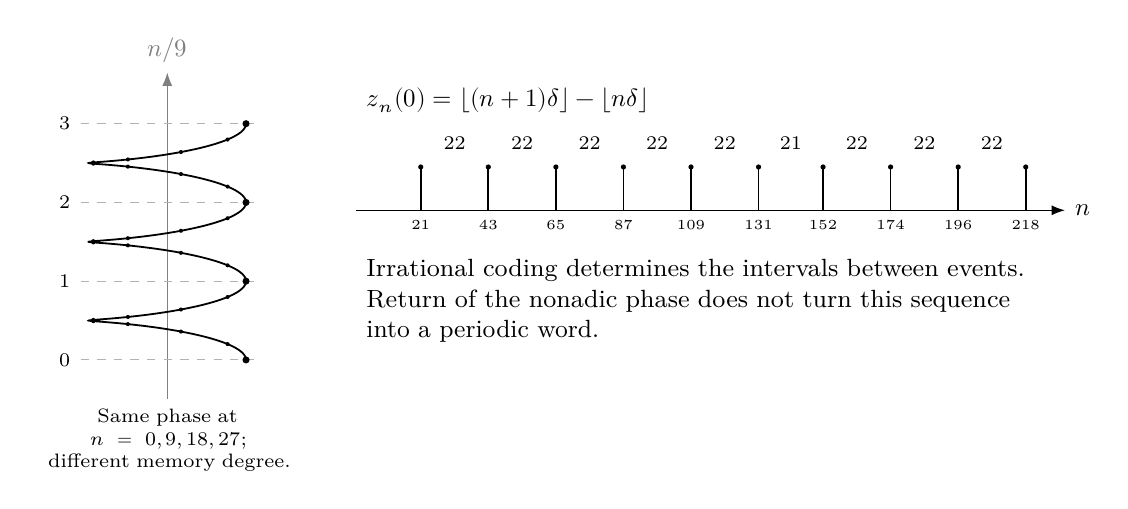
\begin{tikzpicture}[x=1cm,y=1cm,>=Latex,font=\small]
\begin{scope}[xshift=1.8cm,yshift=.3cm]
\draw[->,gray] (0,-.5)--(0,3.65) node[above] {\(n/9\)};
\foreach \k in {0,1,2,3}{
 \draw[gray!60,dashed] (-1.1,\k)--(1.1,\k);
 \node[left,font=\scriptsize] at (-1.1,\k){\(\k\)};
}
\draw[black,line width=.65pt,domain=0:27,samples=260,smooth,variable=\n]
 plot ({cos(40*\n)},{\n/9+.14*sin(40*\n)});
\foreach \n in {0,...,27}{
 \fill ({cos(40*\n)},{\n/9+.14*sin(40*\n)}) circle (.026);
}
\foreach \k in {0,1,2,3}{\fill (1,\k) circle (.045);}
\node[align=center,text width=3.3cm,font=\scriptsize] at (0,-1.02)
 {Same phase at \(n=0,9,18,27\);\\different memory degree.};
\end{scope}
\begin{scope}[xshift=4.2cm,yshift=.5cm]
\node[anchor=west] at (0,3.1){\(z_n(0)=\lfloor(n+1)\delta\rfloor-\lfloor n\delta\rfloor\)};
\draw[->] (0,1.7)--(9,1.7) node[right]{\(n\)};
\foreach \n in {21,43,65,87,109,131,152,174,196,218}{
 \draw[line width=.6pt] ({\n*.039},1.7)--({\n*.039},2.25);
 \fill ({\n*.039},2.25) circle (.033);
 \node[below,font=\tiny] at ({\n*.039},1.7){\n};
}
\foreach \a/\b/\g in {21/43/22,43/65/22,65/87/22,87/109/22,109/131/22,131/152/21,152/174/22,174/196/22,196/218/22}{
 \node[font=\scriptsize] at ({(\a+\b)*.0195},2.55){\g};
}
\node[anchor=west,align=left,text width=8.3cm] at (0,.55)
 {Irrational coding determines the intervals between events. Return of the nonadic phase does not turn this sequence into a periodic word.};
\end{scope}
\end{tikzpicture}
\caption{Complementary representations of transport. Left: projection of the helix \((\cos(2\pi n/9),\sin(2\pi n/9),n/9)\): advancing nine steps recovers the phase and increases the height. Right: the first ten events of the lower word for \(\delta=\log_{10}(10/9)\), with exact separations \(21\) or \(22\). The helical representation introduces no additional physical metric.}
\label{fig:holonomia-esturmiana}
\end{figure}


For this count we fix the intercept \(\theta=0\) and the accumulated endpoints \((N_0,\ldots,N_4)=(0,729,972,999,1000)\), corresponding to the cubic order \((729,243,27,1)\). The lower counts are \(\lfloor N_j\delta\rfloor-\lfloor N_{j-1}\delta\rfloor\), and give \((33,11,1,0)\). The upper counts are \(\lceil N_j\delta\rceil-\lceil N_{j-1}\delta\rceil\), with the same initial boundary zero, and give \((34,11,1,0)\). These values depend on the intercept and the ordering of the strata; they are not asserted for an arbitrary initial phase. Their totals are forty-five and forty-six. The increment corresponds to a single boundary unit, located in the first stratum of this ordered partition. The numbers thirty-four and eleven thus appear in a single count preceding any chart of units; identifying them with physical exponents additionally requires the corresponding dimensional derivation.

The term \emph{aperiodic crystal} is used here for this symbolic order, with its complexity, spectrum, and return specified. Zero topological entropy does not by itself amount to zero physical dissipation: a thermodynamic realization requires a defined energy dynamics and erasure operation. Likewise, this Sturmian reading does not replace all TPK operators or by itself prove periodicity or aperiodicity of the complete output of \(\alpha\). Its function is to make explicit an order structure not described by the simple return of the calendar.

% Cumulative addition. Insert after the existing Sturmian suspension.
% Preserve the complete text and figure fig:holonomia-esturmiana.
\subsection{Nonadic connection, holonomy, and monodromic representation}
\label{mono-ampl:conexion}

The already constructed regional connection is now studied through three objects:
transport of the complete state, the representation of its turns, and the
suspension of its itineraries. The APP--TRIT--TPK operations and the
initial catalog retain their preceding definitions. The necessary
distinction here concerns what each representation retains of the
same history.

At prolongation index \(k\), a state chart preserves
\[
 \widehat x_k=(B_k,C_k,p_k,c_k,\Sigma_k,W_k,g_k,m_k).
\]
Here \(B_k\) brings together the three regional blocks, \(C_k\) is the cylinder,
\(p_k\) the prefix, \(c_k\) the carry record, \(\Sigma_k\) the boundary
signature, and \(W_k\) the incidence information. The phase is
\(g_k=1+[(k-1)]_9\); \(m_k\) counts complete turns. The reduction
\(\beta_k=[m_k]_{12}\) preserves the dodecaphase position, whereas the
integer \(m_k\) distinguishes its successive turns.

\begin{definition}[Transport through one nonadic turn]
\label{mono-ampl:def-vuelta}
Let \(\mathcal R_k\subseteq\widehat X_k\times\widehat X_{k+1}\)
be the admissible-extension relations of the TPK. The realization of
holonomy at level \(k\) is the relational composition
\[
 \Gamma_{9,k}=\mathcal R_{k+8}\circ\cdots\circ\mathcal R_k.
\]
For \(s\geq1\), its prolongation to \(s\) turns is
\[
 \Gamma_{9s,k}=
 \Gamma_{9,k+9(s-1)}\circ\cdots\circ\Gamma_{9,k}.
\]
\end{definition}

The relational formulation preserves admissible continuations. On
an individualized history, each arrow leads to the state actually
prolonged; the isolated visible block may still admit more than one
continuation. This difference is precisely the function of memory and
boundary conditions in determining the trajectory.

\begin{proposition}[Iteration of return and accumulated memory]
\label{mono-ampl:vueltas}
In every admissible composition of \(s\) turns,
\[
 g_{k+9s}=g_k,\qquad m_{k+9s}=m_k+s,\qquad
 \beta_{k+9s}=\beta_k+s\pmod{12}.
\]
\end{proposition}
\begin{proof}
The one-turn rule preserves phase and increases the counter by one
unit. Applying it to the already transported state repeats exactly those
two operations. Induction gives the first two equalities; reducing the
second modulo \(12\) gives the third.
\end{proof}

The counter thus provides an integer witness to the difference between
turns. After \(12\) turns the pair of finite phases is restored, but
the counter increases by \(12\). The nonsplit extension
\eqref{eq:extension108} expresses the composition of the calendar through its
cocycle; the trajectory additionally retains the integer lift of that datum.
Conservation here means transport of previous contributions,
not immobility of every coordinate.

\subsubsection{Bilateral representation of the return index}

The shift \(T\) in \eqref{eq:weyl-relojes} admits an
expression in phase and turn coordinates. We number phases from \(0\) to
\(8\), by shifting the origin relative to \(g_k\), and
write \(k=9m+r\), with \(0\leq r<9\), on the integer line
covering the phase cycle. On
\(\mathcal H_{\rm ind}=\ell^2(\mathbb Z)\), the basis
\(|k\rangle=|r,m\rangle\) expresses that same unitary shift
\[
 T|r,m\rangle=
 \begin{cases}
 |r+1,m\rangle,&r<8,\\
 |0,m+1\rangle,&r=8.
 \end{cases}
\]
The inverse reduces \(r\) by one unit when \(r>0\), and sends
\(|0,m\rangle\) to \(|8,m-1\rangle\). Passage through the phase origin
therefore incorporates the exact quotient unit.

\Needspace{8\baselineskip}
\begin{proposition}[Representation of the monodromy of the cycle]
\label{mono-ampl:representacion}
Let \(S=T^9\). Then
\[
 S|r,m\rangle=|r,m+1\rangle,\qquad
 \mathbb Z\longrightarrow\mathcal U(\mathcal H_{\rm ind}),
 \quad s\longmapsto S^s
\]
is a faithful unitary representation of the turn group of the cycle.
\end{proposition}
\begin{proof}
Nine shifts preserve the remainder of division by \(9\) and
increase the quotient. The powers satisfy
\(S^{s+t}=S^sS^t\), and \(S^s|r,m\rangle=|r,m+s\rangle\) distinguishes
every integer \(s\). A permutation of an orthonormal basis is unitary.
\end{proof}

This representation corresponds to the covering of the cycle, whose turn
group is \(\mathbb Z\), and represents phase together with its counter. The
TPK state additionally contains the trajectory coordinates already described.
The bilateral extension admits negative indices as coordinates of the
covering; a trajectory starting from an initial condition uses
its admissible half-axis. This provides an operator inverse
of the index without turning every extension relation into a bijection of the
complete state.

With \(D_M|k\rangle=\lfloor k/9\rfloor|k\rangle\), the identity
\([D_M,S]=S\) expresses the memory increment on the dense domain of
finitely supported vectors. If \(\mathcal I|k\rangle=|-k\rangle\) and
\(P_0\) projects onto indices divisible by \(9\), one additionally obtains
\begin{equation}
 \mathcal I T\mathcal I=T^{-1},\qquad
 \mathcal I D_M\mathcal I=-D_M-(I-P_0).
 \label{mono-ampl:inversion-contador}
\end{equation}
Indeed, for \(k=9m+r\),
\(\lfloor-k/9\rfloor=-m\) if \(r=0\) and equals \(-m-1\) if \(r>0\).
Inversion thus preserves the boundary term of Euclidean division.

\subsection{Block clock and capacity clock}
\label{mono-ampl:relojes}

The index of an application of refinement and the number of available
decimal positions have related but different laws. To
express them, we reserve \(n\) for the ternary-block index and define
\[
 \rho=\log_{1000}729=\log_{10}9,\qquad
 \delta=1-\rho,\qquad
 \mathcal C_n=\lfloor(n+1)\rho\rfloor,\quad n\geq0.
\]
The letter \(\mathcal C_n\) here designates capacity, not the dodecaphase
record \(K\). At the canonical phase origin, the preceding mechanical
word provides
\[
 Z_n=\sum_{j=0}^{n}z_j(0)=\lfloor(n+1)\delta\rfloor.
\]

\begin{proposition}[Exact balance between capacity and vacancies]
\label{mono-ampl:balance-capacidad}
For \(n\geq0\) and, in the second identity, \(n\geq1\),
\[
 \mathcal C_n=n-Z_n,\qquad
 \mathcal C_n-\mathcal C_{n-1}=1-z_n(0).
\]
\end{proposition}
\begin{proof}
The irrationality of \(\delta\) implies
\(\lceil(n+1)\delta\rceil=\lfloor(n+1)\delta\rfloor+1\).
Then
\[
 \lfloor(n+1)(1-\delta)\rfloor
 =n+1-\lceil(n+1)\delta\rceil=n-Z_n.
\]
Subtracting two consecutive identities completes the proof.
\end{proof}

An event \(z_n=1\) adds a block to the history while maintaining capacity
\(\mathcal C_n\); an event \(z_n=0\) increases both counters. In
any interval, capacity increments and vacancies sum to
exactly its length. Reducing modulo \(q\), for \(q=9\) or
\(q=108\), gives
\[
 [\mathcal C_n]_q=[n]_q-[Z_n]_q.
\]
The uniform block phase and the capacity phase are related through
the integrated memory of vacancies. In particular, a retention of
capacity and a complete turn of the connection have different
mechanisms, although both may preserve a phase observation.

Monotone inversion of the clock gives a first-arrival time:
\[
 T_{\rm cap}(a)=\min\{n:\mathcal C_n=a\}
 =\left\lceil\frac a\rho\right\rceil-1,
 \qquad a\geq1.
\]
With \(\sigma=\rho^{-1}-1\), the time taken to gain \(b\) units
of capacity is
\[
 T_{\rm cap}(a+b)-T_{\rm cap}(a)
 =b+\lceil(a+b)\sigma\rceil-\lceil a\sigma\rceil.
\]
The difference of ceilings takes one of the two integers adjacent to
\(b\sigma\). Thus \(9\) or \(10\) blocks are obtained to gain
\(9\) units of capacity, and \(113\) or \(114\) to gain \(108\).
These are times of the inverse clock, measured from a first arrival; the
turn counter is always interpreted in the index to which it belongs.

\subsection{Symbolic suspension and aperiodic time crystal}
\label{mono-ampl:cristal}

Rotation coding combines phase periodicity, local recurrence,
and global aperiodicity. Let \(\mathcal X_\delta\subseteq\{0,1\}^{\mathbb Z}\)
be the closure, in the product topology, of the translates of the
bilateral word \(z_n(\theta)\). Denote by \(\sigma_{\rm sh}\) the
shift of its sequences. Retaining a nonadic phase, the step is
\[
 F(r,z)=([r+1]_9,\sigma_{\rm sh}z),\qquad
 (r,z)\in C_9\times\mathcal X_\delta.
\]

\begin{definition}[Symbolic aperiodic time crystal]
\label{mono-ampl:def-cristal}
The unit-roof suspension of the preceding system is the space
\[
 \mathcal S_\delta=
 \bigl((C_9\times\mathcal X_\delta)\times\mathbb R\bigr)/\sim,
 \qquad (y,t+1)\sim(Fy,t),
\]
with flow \(\Phi_s[y,t]=[y,t+s]\). This model of temporal order,
together with its vacancy coding and representation of the turn counter,
is called a \emph{symbolic aperiodic time crystal}.
\end{definition}

The adjective temporal designates the action of the flow and its return section;
aperiodicity characterizes its itineraries. The frequency of ones in every
sequence is \(\delta\): the uniform discrepancy bound of less than one,
obtained by telescoping in any window, persists on taking the closure.
A periodic sequence would have rational frequency. Therefore,
\(\mathcal X_\delta\) contains no periodic orbits. The suspension
also has no closed orbits: a return of the flow would require an integer
time and periodicity of the itinerary.

Finite words do recur. Itineraries of length \(m\)
arise from a partition of the circle by \(m+1\) points; each
interval is visited recurrently by the irrational rotation. Even
when times are restricted to a fixed phase, the step \(9\delta\) remains
irrational. This is why every word appears in all
\(9\) phases, and explains the already established complexities
\[
 p(m)=m+1,\qquad p_9(m)=9(m+1),\qquad p_3(m)=3(m+1).
\]
Recurrence of local configurations coexists with the absence of a
global period. Its topological entropy is zero because these complexities
grow linearly.

Realization through the observables \(V_9,W_\delta\) and shift
\(T\) expresses the same order through the covariances
\eqref{eq:weyl-relojes}. Frequencies of the uniform clock belong to
\(\frac19\mathbb Z+\delta\mathbb Z\), modulo \(1\). The capacity clock
additionally preserves the relation
\([\mathcal C_n]_9=[n]_9-[Z_n]_9\); it is not replaced by the uniform phase
when interpreting returns. The term \emph{time crystal} is thus
defined through a mathematical dynamical system. Its physical realization
requires specification of an energy dynamics, its temporal observables,
and its stability, data distinct from the present symbolic construction.

\subsection{Specular symmetry of the regions and double realization}
\label{mono-ampl:regiones}

Specular exchange acts on the regional block
\(B=(u^\pi,u^e,u^\varphi)\in(\mathbb F_3^6)^3\) by
\[
 \mathfrak cB=(u^e,u^\pi,u^\varphi).
\]
Its fixed axis and aggregate are, respectively, \(u^\varphi\) and
\(s=u^\pi+u^e\). This fixation refers to the involution within a fiber;
both coordinates may evolve during nonadic transport.
With \(q=u^\pi+u^e+u^\varphi\),
\(a=u^\pi+u^e-u^\varphi\), and \(d=u^\pi-u^e\), one recovers
\[
 u^\varphi=2(q-a),\qquad s=q-u^\varphi,\qquad
 u^\pi=2(s+d),\qquad u^e=2(s-d).
\]
The equalities hold componentwise in \(\mathbb F_3\), where
\(2^{-1}=2\). The mirror preserves \(q,a,s\) and reverses \(d\); this
antisymmetric coordinate individualizes the distribution that the aggregate preserves
without distinguishing it. The inversion \(\mathcal I\) of the temporal index and the
channel involution \(\mathfrak c\) consequently act on
different data.

Phase return has an explicit witness:
\[
 \begin{aligned}
 B_1&=(012222\mid121221\mid112202),\\
 B_{10}&=(101222\mid112221\mid112002).
 \end{aligned}
\]
Both positions have phase \(1\); the block, axis, and memory have
changed. Likewise, synchronization of the censuses at phases \(8\) and
\(9\) cancels their relative differences, while the diagonal component
passes from \((59,59,59)\) to \((43,43,43)\). Equality of a relative
observable does not exhaust the state determining it.

Double realization preserves that architecture. In Section
\ref{exc:doble-lectura}, the same prefix determines nested
cylinders on the one hand and a sequence of coded words with their frames on the other.
The first map passes to the limit by contraction of diameters; the second
satisfies \(r_{n,m}Q_n=Q_mp_{n,m}\) and defines \(Q_\infty\).
Figure \ref{mono-ampl:fig-regional} anticipates these two maps.
The subsequent incidence development constructs codes, lattices, and the
realization of Moonshine in their own domains; the automorphism group
acts on that realization, not on the digits through an implicit
identification.

% Figura acumulativa; destino figures/monodromia_regional_ampliacion.tex.
\begin{figure}[!htbp]
\centering
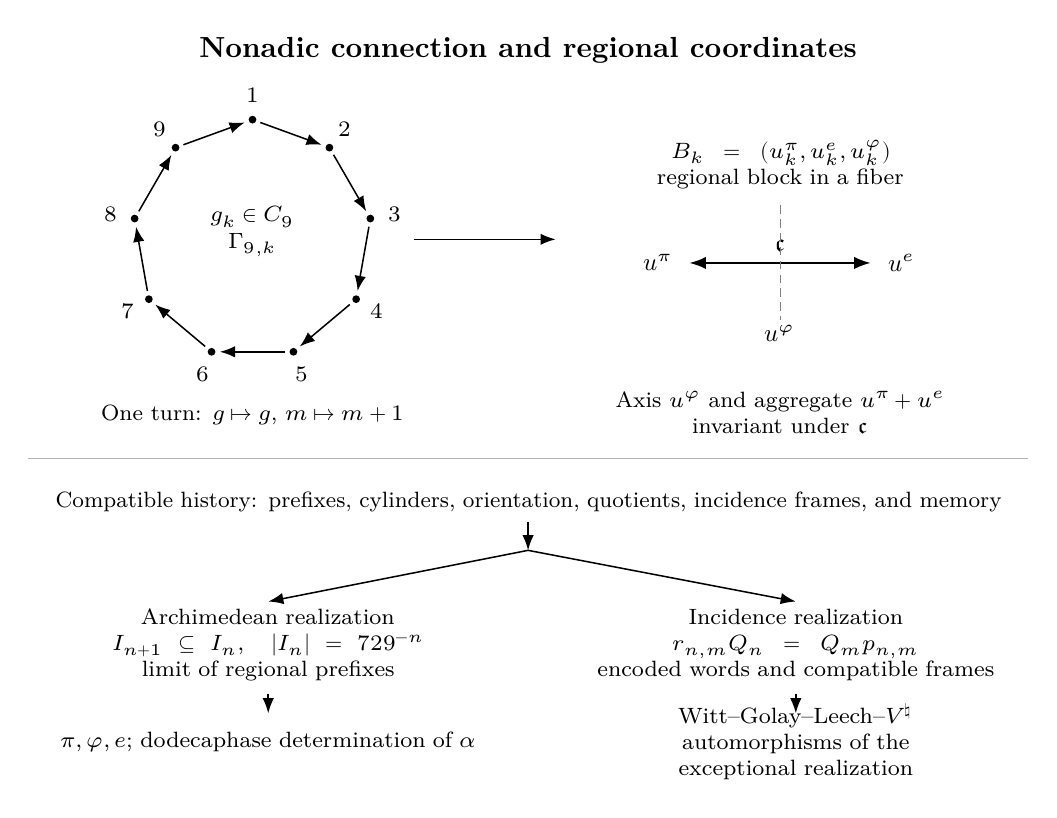
\begin{tikzpicture}[x=1cm,y=1cm,>=Latex,font=\small,
  flow/.style={->,line width=.55pt},
  ann/.style={align=center,font=\footnotesize}]
\node[font=\bfseries] at (6.9,9.2)
  {Nonadic connection and regional coordinates};
\begin{scope}[shift={(3.4,6.8)}]
 \foreach \k in {1,...,9}{
  \pgfmathsetmacro{\ang}{90-40*(\k-1)}
  \coordinate (p\k) at (\ang:1.52);
  \fill (p\k) circle (1.4pt);
  \node[fill=white,inner sep=1.1pt,font=\footnotesize]
    at (\ang:1.83) {\(\k\)};
 }
 \foreach \k in {1,...,8}{
  \pgfmathtruncatemacro{\next}{\k+1}
  \draw[flow,shorten >=3pt,shorten <=3pt] (p\k)--(p\next);
 }
 \draw[flow,shorten >=3pt,shorten <=3pt] (p9)--(p1);
 \node[ann] at (0,.1) {\(g_k\in C_9\)\\\(\Gamma_{9,k}\)};
 \node[ann] at (0,-2.23) {One turn: \(g\mapsto g\), \(m\mapsto m+1\)};
\end{scope}
\node[ann,text width=5.25cm] at (10.1,7.75)
 {\(B_k=(u_k^\pi,u_k^e,u_k^\varphi)\)\\
 regional block in a fiber};
\node at (8.55,6.5) {\(u^\pi\)};
\node at (11.65,6.5) {\(u^e\)};
\draw[<->,line width=.65pt] (8.95,6.5)--node[above]{\(\mathfrak c\)}(11.25,6.5);
\draw[densely dashed,gray] (10.1,5.72)--(10.1,7.23);
\node[fill=white,inner sep=2pt] at (10.1,5.6){\(u^\varphi\)};
\node[ann] at (10.1,4.6)
 {Axis \(u^\varphi\) and aggregate \(u^\pi+u^e\)\\
 invariant under \(\mathfrak c\)};
\draw[flow] (5.45,6.8)--(7.25,6.8);
\draw[gray!60,line width=.3pt] (.55,4.02)--(13.25,4.02);
\node[ann,text width=12cm] (hist) at (6.9,3.47)
 {Compatible history: prefixes, cylinders, orientation, quotients,
 incidence frames, and memory};
\coordinate (fork) at (6.9,2.85);
\draw[flow] (hist.south)--(fork);
\draw[flow] (fork)--(3.6,2.2);
\draw[flow] (fork)--(10.3,2.2);
\node[ann,text width=5.6cm] at (3.6,1.65)
 {Archimedean realization\\
 \(I_{n+1}\subseteq I_n,\quad |I_n|=729^{-n}\)\\
 limit of regional prefixes};
\node[ann,text width=5.6cm] at (10.3,1.65)
 {Incidence realization\\
 \(r_{n,m}Q_n=Q_mp_{n,m}\)\\
 encoded words and compatible frames};
\node[ann,text width=5.6cm] at (3.6,.42)
 {\(\pi,\varphi,e\); dodecaphase determination of \(\alpha\)};
\node[ann,text width=5.6cm] at (10.3,.42)
 {Witt--Golay--Leech--\(V^\natural\)\\
 automorphisms of the exceptional realization};
\draw[flow] (3.6,1.03)--(3.6,.78);
\draw[flow] (10.3,1.03)--(10.3,.78);
\end{tikzpicture}
\caption{\fontsize{9}{11}\selectfont Nine phases of a connection and two realizations of a compatible
history. The cycle represents phase; each turn increments the counter.
The regional diagram represents the involution \(\mathfrak c\), which
interchanges closure and propagation and fixes the self-scaling axis in a fiber.
This invariance does not require the axis to remain constant during transport.
The two lower maps use the same prefix: one determines its numerical limit,
while the other preserves words and incidence frames. The maps of the second
realization are specified in Section \ref{exc:doble-lectura}; the exceptional
construction is developed afterwards.}
\label{mono-ampl:fig-regional}
\end{figure}


\clearpage
\subsubsection{Rectilinear representation of phases and return}
\label{mono-recta:desarrollo}

The representation on the segment \([0,10]\) preserves the positional
origin of APP and orders its nine interior marks. In this diagram,
the integers \(1,\ldots,9\) are phase representatives. Horizontal
position indicates the order of the charts; upper labels
specify regional operations. Figure
\ref{mono-recta:figura} thus brings together the initial line, fixation of the
self-scaling axis, the specular distribution of the two channels, and
return with memory.

\input{figures/recta_nonadica_0_10.tex}

Fixation of the axis is formulated in the fiber of a given boundary. If
\(q=u^\pi+u^e+u^\varphi\) and
\(a=u^\pi+u^e-u^\varphi\), then
\[
 u^\varphi=2(q-a),\qquad s=u^\pi+u^e=q-u^\varphi
 \quad\text{in }\mathbb F_3^6.
\]
The data \((q,a)\) determine the axis and aggregate; the ordered distribution
of \(s\) retains the specular freedom resolved by prolongation.
The fifth phase has a local solution and an extension, with boundary
datum \(c=111111\) and residual signature \(\rho_W=000\). This is the
meaning of its first strong saturation. The symbol \(\varphi\)
placed above the mark \(5\) identifies the regional axis entering
that operation.

The intermediate phases preserve this decomposition within each fiber,
while their boundary data evolve. The complete census of local
multiplicities and extensions of the distinguished branch is
\[
\begin{array}{c|rrrrrrrrr}
\text{phase}&1&2&3&4&5&6&7&8&9\\\hline
N_{\rm loc}&3&2&5&4&1&1&3&3&2\\
N_{\rm ext}&2&5&4&1&1&3&3&2&1
\end{array}
\]
Phase \(6\) combines local uniqueness and three prolongations; phase
\(7\) resolves a triple specular fiber; phase \(8\) synchronizes
the three regional censuses. Phase \(9\) preserves two local
distributions with the same axis and aggregate, one of which
prolongs. These counts express different functions within a
single connection and justify the marks on the line.

In particular, for phases \(6,7,8\), the regional sums are
respectively \(012100\), \(101001\), and \(112000\). The conservation
represented by the brace is an invariance under the specular
distribution within each fiber. Subsequent real evaluation applies the
readers of compatible cylinders to complete histories; the
internal sum represented in the figure belongs to the ternary domain.

Finally, the arc \(9\to1\) represents passage from one turn to the
next. The formulas of Section
\ref{mono-ampl:conexion} preserve the phase remainder and increase the
turn counter. The rectilinear diagram and the cyclic diagram in
Figure \ref{mono-ampl:fig-regional} therefore express two complementary
aspects of the same holonomy: the order of positions and
composition of the return on the state with memory.


\subsection{Temporal transport and tritic exponential composition}
\label{mono-ampl:euler}

The Euler relations of Section \ref{euler-trit-articulacion}
describe local realizations of the three regimes. For a fixed
signature \(\tau\), the generator satisfies \(J_\tau^2=-\tau I\);
algebraic conjugation sends \(J_\tau\) to \(-J_\tau\). Consequently,
\[
 \exp(sJ_\tau)\exp(tJ_\tau)=\exp((s+t)J_\tau),\qquad
 \overline{\exp(tJ_\tau)}=\exp(-tJ_\tau),
\]
and the product of an evolution with its conjugate is unity. In the elliptic
type this is realized through \(\cos^2t+\sin^2t=1\); in the hyperbolic type,
through \(\cosh^2t-\sinh^2t=1\); in the parabolic type,
\((I+tN)(I-tN)=I\), since \(N^2=0\). The same conservation law
admits three quadratic expressions.

The elliptic realization closes a turn; the nilpotent one preserves a
linear displacement; the hyperbolic one separates expansion and contraction with
unit determinant. At the already generated regional parameters,
\[
 \exp(\pi J_{\mathrm e})=-I,\qquad
 \exp(J_{\mathrm p})=I+J_{\mathrm p},\qquad
 \exp(2\log\varphi\,J_{\mathrm h})=F_{\rm av}^{\,2}.
\]
The evaluation \(\exp(I)=eI\) recognizes unity in the common
exponential law. The number \(e\) is not assigned exclusively to the parabolic regime.

Transport of a local realization by an isomorphism \(U\) preserves
these relations: if \(J'=UJU^{-1}\), the exponential series gives
\(U\exp(tJ)=\exp(tJ')U\). The identity transports the regime and its
norm. A transition between different quadratic types belongs, by contrast,
to the TPK selection of sheets and regimes; it is not a conjugation
changing the value of \(J^2\). The temporal product therefore preserves the
order of transitions and the information at their endpoints.

This articulation distinguishes closure of a local representation from
holonomy of a history. The identity \(\exp(2\pi J_{\mathrm e})=I\) may hold
at the same time as \(S|r,m\rangle=|r,m+1\rangle\). The first equality
restores the orientation of the regime; the second records another turn. The
discrete structure preserves both: local return and the accumulated
provenance of the state realizing it.


% Recovery of the native product and its selector, not incorporation of RH.
\subsection{Multiplicative irreducibility and return periods}
\label{primos-retornos}

The distinction between structure, evaluation, and phase also appears in
the multiplicative sector. APP's local product contains both residue and
quotient; iterating it constructs normal forms and factorizations before
their decimal periods are examined. This development places the expression
\emph{prime mode} in a precise domain and relates irreducibility to the
operations already defined, rather than to an isolated coincidence
of periods.

Let
\[
 \mathcal W_9=\{\varnothing\}\sqcup
 \bigsqcup_{\ell\geq1}\{1,\ldots,9\}^{\ell}.
\]
Sequences are ordered from the least significant digit. The evaluation
\(\operatorname{ev}_9(u)=\sum_j u_j9^j\), with
\(\operatorname{ev}_9(\varnothing)=0\), is bijective onto the nonnegative
integers: for a positive integer, division of \(n-1\) by \(9\)
uniquely determines the first digit and continuation. This is bijective
nonadic numeration; it retains the boundary representative \(9\).

Addition \(\boxplus_\#\) is obtained by applying APP's additive sheet
to the digits at each position and propagating their quotients. If there
is only one digit, it is the provisional residue; a nonzero incoming
quotient is normalized through a second additive operation. The sum of
quotients is transported to the next position. To multiply a sequence by
a digit \(d\), the multiplicative cell produces
\(u_jd=9q_j+r_j\), and the incoming quotient \(c_j\) is incorporated by
\[
 (w_j,c_{j+1})=
 \begin{cases}
 (r_j,q_j),&c_j=0,\\
 \bigl(R^+(r_j,c_j),q_j+q^+(r_j,c_j)\bigr),&c_j>0.
 \end{cases}
\]
Start with \(c_0=0\) and incorporate the final quotient when nonzero.
During addition, \(c_j\leq2\); during multiplication by a digit,
\(c_j\leq9\). Local operations thus receive arguments within
their domain. Denote this second procedure by \(d\odot_\#u\),
with \(d\odot_\#\varnothing=\varnothing\).

For \(v=(v_0,\ldots,v_{m-1})\), the complete product is constructed
through the recurrence
\[
 a_m=\varnothing,\qquad
 a_j=(9\odot_\#a_{j+1})\boxplus_\#(v_j\odot_\#u),
 \qquad u\boxtimes_\#v=a_0.
\]
The rule composes both local sheets. Its evaluation satisfies
\begin{equation}
 \operatorname{ev}_9(u\boxtimes_\#v)
   =\operatorname{ev}_9(u)\operatorname{ev}_9(v).
 \label{eq:primos-entrelazamiento}
\end{equation}
Indeed, each transition preserves the partial sum plus the pending
quotient weighted by the power of \(9\). The recurrence then gives
\(\operatorname{ev}_9(a_j)=9\operatorname{ev}_9(a_{j+1})+
v_j\operatorname{ev}_9(u)\), whose iteration proves
\eqref{eq:primos-entrelazamiento}. Uniqueness of normal form transports
associativity and commutativity to the constructed product; its identity is \((1)\).

\begin{definition}[Reduced multiplicative coproduct]
On the finitely supported vector space generated by nonempty normal
forms, define
\[
 \widetilde\Delta_\# e_w
 =\sum_{\substack{u\boxtimes_\#v=w\\u,v\ne(1)}}e_u\otimes e_v.
\]
A non-unit normal form is irreducible when its image under
\(\widetilde\Delta_\#\) is zero.
\end{definition}

Factorization fibers are finite by
\eqref{eq:primos-entrelazamiento}. In the completion
\(\mathcal H_\#=\ell^2(\mathcal W_9\setminus\{\varnothing\})\),
images of distinct forms have disjoint supports. If \(d_\#(w)\)
counts ordered non-unit factorizations, the domain of the closure is
\[
 \operatorname{Dom}(\overline{\widetilde\Delta_\#})
 =\left\{x\in\mathcal H_\#:
       \sum_w d_\#(w)|x_w|^2<\infty\right\}.
\]
Indeed, the squared norm of the image is this weighted sum. Hence
the operator
\[
 A_\#=(\overline{\widetilde\Delta_\#})^*
                  \overline{\widetilde\Delta_\#}
\]
is diagonal, positive, and self-adjoint: its eigenvalue at \(e_w\)
is the number of ordered non-unit factorizations of \(w\). The projection
\[
 P_{\rm irr}=(I-|e_{(1)}\rangle\langle e_{(1)}|)
                    \mathbf1_{\{0\}}(A_\#)
\]
selects exactly the irreducible forms. Through multiplicative evaluation,
these correspond to ordinary primes. Selection depends on factorization
structure and keeps the unit state separate.

For a value \(n\geq2\) coprime to \(10\), decimal division induces
the residue permutation \(r\mapsto10r\pmod n\). Return of residue
\(1\) has period
\[
 \tau_n=\operatorname{ord}_n(10).
\]
If \(n=\prod_p p^{a_p}\), the Chinese remainder theorem gives
\[
 \tau_n=\operatorname{lcm}_{p^{a_p}\parallel n}
                    \operatorname{ord}_{p^{a_p}}(10).
\]
Composite return synchronizes the returns of prime powers.
For a prime \(p\notin\{2,3,5\}\),
\[
 \tau_p\mid p-1,\qquad
 M_p=\frac{10^{\tau_p}-1}{p}\in\mathbb N,
 \qquad M_p\equiv0\pmod9.
\]
The last congruence expresses nonadic closure of decimal repetition:
\(10^{\tau_p}-1\) is a multiple of \(9\), and \(p\) is invertible
modulo \(9\). The same congruence holds for every \(n\) coprime
to \(90\). In particular, \(7,13,77,91,143\) have decimal period
\(6\), although only the first two are irreducible. The coproduct and
the period therefore record different properties of the same constructed value.

This differentiation specifies the relation with aperiodic refinement.
The vacancy sequence determines increments of the capacity index;
factorization determines multiplicative modes; decimal division
determines their return times. The nonadic representative preserves
phase closure, while quotient and factorization retain information
that this closure does not distinguish. The connection to the treatise's
spectral constructions resides in these operators and their intertwinings.
Proof of their subsequent analytic results retains its own development;
it is not replaced by periodicity of a residue observation.

\subsubsection{Vacancy discrepancy and Dirichlet readings}

The connection also admits an exact analytic expression. Retain the
same coding \(z_n=z_n(0)\), for \(n\geq1\), and consider two
subsequent observables: the series over all indices and the product
over indices selected by irreducibility. For \(\operatorname{Re}s>1\),
\[
 Z_{\rm vac}^{+}(s)=\sum_{n\geq1}\frac{z_n}{n^s},\qquad
 Z_{\rm vac}^{\times}(s)=\prod_p(1-p^{-s})^{-z_p}.
\]
Both converge absolutely in this half-plane. Their common factor is
density \(\delta\), but their discrepancies differ.

\Needspace{21\baselineskip}
\begin{proposition}[Separation of vacancy density]
We have
\[
 Z_{\rm vac}^{+}(s)=\delta\zeta(s)+H_{\rm vac}(s),
 \qquad H_{\rm vac}\in\mathcal O(\operatorname{Re}s>0).
\]
In \(\operatorname{Re}s>1\), with logarithms defined by absolutely
convergent Euler series,
\[
 Z_{\rm vac}^{\times}(s)=\zeta(s)^\delta G_{\rm vac}(s),\qquad
 \log G_{\rm vac}(s)=
 \sum_p(z_p-\delta)\log(1-p^{-s})^{-1}.
\]
\end{proposition}
\begin{proof}
The centered partial sums satisfy
\[
 A_N:=\sum_{n=1}^N(z_n-\delta)
 =\lfloor(N+1)\delta\rfloor-N\delta,\qquad |A_N|<1.
\]
Abel summation represents the centered term by
\(s\int_1^\infty A_{\lfloor x\rfloor}x^{-s-1}\,dx\).
The integral converges locally uniformly in \(\operatorname{Re}s>0\),
proving holomorphy. The second identity follows by separating
\(z_p=\delta+(z_p-\delta)\) in the logarithm of the product,
within its domain of absolute convergence.
\end{proof}

The decomposition reveals what the reading on primes adds: it examines
the same vacancy sequence on a subset determined by factorization.
Controlling discrepancy over all integers gives the first holomorphic
continuation; the second observable preserves its own discrepancy on
primes. These are two applications of the same discrete structure,
with explicit analytic domains. This articulation explains their
relevance to the arithmetic kernel without transferring the proof
of the treatise's terminal results to this article.


\clearpage
% BEGIN NUCLEO_ADITIVO_20260921_SELECCION
\clearpage
% Demonstrative expansion DF003--DF007. The integral source is unchanged.
% Common owner of the Lean files cited in these comments:
% output/PAQUETE_ARTICULO_I_INTEGRACION_ESTADO_CAMPOS_20260919/.
% Causal placement of the first section: after the coinductive regional
% readers and before their registers are used as inputs to K selection.
% Causal placement of the second section: after the marked
% Paley--Witt--Golay--Leech construction and before reconstruction of the VOA.
% Both expository cuts preserve the same APP--TRIT--TPK origin.

\section[Regional generation and refinement]{Integral compatibility of regional generation, cylindrical refinement, and incidence}
\label{act21:sec:df-lectores-cilindros}

Regional prolongation produces ordered sequences of blocks together with
their reading depths. The Archimedean projection and ternary incidence
are calculated on these same sequences. The connection between the two
realizations can be formulated entirely through integer operations:
selection by rational intervals, Euclidean division, lifting of six
trits, carry reading, and the Witt transformation. This formulation makes
it possible to trace each coefficient from its generating block to its
subsequent use.

The construction uses the three regional readers already obtained from the
APP--TRIT--TPK state. We denote them by the indices
\(c\in\{\mathrm P,\mathrm E,\mathrm F\}\), corresponding, respectively,
to the closure, propagation, and autoscaling regions. Their real realization
will be written as \(v_c\). The subsequent identifications
\(v_{\mathrm P}=\pi_{\mathrm{HMT}}\),
\(v_{\mathrm E}=e_{\mathrm{HMT}}\), and
\(v_{\mathrm F}=\varphi_{\mathrm{HMT}}\) preserve this causal order.
The operation that emits a block inspects the rational intervals of the
regional reader; the real value enters the proof of correctness of that
operation.

\subsection{Positional emission through rational separation of cells}
\label{act21:subsec:df-emision-racional}

% Source: lean/biblioteca/RegionalPublicationComposition.lean,
% produced_brackets, eventual_publication, joint_eventual_publication,
% search_terminates, stopped_cell_correct, publications_compatible.

For each region, two rational sequences
\(\ell_c(j),u_c(j)\), constructed by its reader, are available and satisfy
\[
 \ell_c(j)\leq v_c\leq u_c(j).
\]
The cell-separation property proved for these readers states that, for
each integer \(s>0\), there exists \(J\) such that, for every \(j\geq J\),
\begin{equation}
 \lfloor s\ell_c(j)\rfloor
 =\lceil su_c(j)\rceil-1
 =\lfloor sv_c\rfloor.
 \label{act21:eq:df-separacion-celdas}
\end{equation}
Avoidance of rational boundaries by the regional values is the hypothesis
of the preceding theorems that guarantees this separation. Here we use
their operational conclusion together with the readers and intervals
that produce it.

\begin{definition}[Separation index and emitted prefix]
For \(s>0\), let
\[
 j_c(s)=\min\{j\in\mathbb N:
 \lfloor s\ell_c(j)\rfloor=\lceil su_c(j)\rceil-1\}.
\]
For an integer base \(b\geq2\) and a depth \(n\geq0\), define
\begin{equation}
 P_c(b,n)=\lfloor b^n\ell_c(j_c(b^n))\rfloor.
 \label{act21:eq:df-publicacion-prefijo}
\end{equation}
The prefix contains the integer part and the first \(n\) positions in base
\(b\); consequently, \(P_c(b,0)\) is the regional integer part.
\end{definition}

\begin{theorem}[Termination and correctness of emission]
\label{act21:thm:df-emision-correcta}
The index \(j_c(s)\) exists for every \(s>0\). The emitted prefixes satisfy
\begin{equation}
 P_c(b,n)=\lfloor b^n v_c\rfloor,
 \qquad
 P_c(b,n)\leq b^n v_c<P_c(b,n)+1.
 \label{act21:eq:df-prefijo-correcto}
\end{equation}
For each scale \(s\), a single sufficiency index \(J(s)\) can also be
chosen that is valid simultaneously for all three regions.
\end{theorem}

\begin{proof}
The eventual equality in \eqref{act21:eq:df-separacion-celdas} makes the set
defining \(j_c(s)\) nonempty. Its minimum exists by the well-ordering of
\(\mathbb N\). At any index where the equality holds, the rational lower
bound gives
\(\lfloor s\ell_c(j)\rfloor\leq\lfloor sv_c\rfloor\).
The upper bound, together with avoidance of a cell boundary, gives
\(\lfloor sv_c\rfloor\leq\lceil su_c(j)\rceil-1\).
When the two integer endpoints coincide, the intervening integer coincides
with them. This proves \eqref{act21:eq:df-prefijo-correcto}. For the joint
statement, it suffices to take the maximum of the three sufficiency indices
obtained at the same scale. The joint index controls all three emissions
simultaneously, while each region retains its own intervals.
\end{proof}

\begin{proposition}[Exact compatibility of prefixes]
\label{act21:prop:df-prefijos-compatibles}
For \(n,m\geq0\),
\begin{equation}
 \left\lfloor\frac{P_c(b,n+m)}{b^m}\right\rfloor=P_c(b,n).
 \label{act21:eq:df-truncamiento}
\end{equation}
In particular, the next block
\(d_c(b,n)=P_c(b,n+1)\bmod b\) satisfies
\begin{equation}
 P_c(b,n+1)=bP_c(b,n)+d_c(b,n),\qquad 0\leq d_c(b,n)<b.
 \label{act21:eq:df-paso-posicional}
\end{equation}
\end{proposition}

\begin{proof}
Write \(b^n v_c=N+\theta\), with
\(N=P_c(b,n)\) and \(0\leq\theta<1\). Then
\(P_c(b,n+m)=b^mN+\lfloor b^m\theta\rfloor\), and the second summand
belongs to \(\{0,\ldots,b^m-1\}\). Euclidean division by \(b^m\)
recovers \(N\). The specialization \(m=1\) yields
\eqref{act21:eq:df-paso-posicional} and its residual bound.
\end{proof}

\subsection{Regional blocks of six trits at arbitrary depth}
\label{act21:subsec:df-bloques-arbitrarios}

% Source: deltas/integracion/JointRegionalFrontier.lean,
% publish_base729_eq_base3, generated_block_from_longer_prefix,
% generated_block_eq_finite, generated_signature_eq_finite.

The integer equality \(729=3^6\) determines the grouping of six ternary
positions into a block. For \(t\geq0\), define
\begin{equation}
 u_c(t)=P_c(729,t+1)\bmod729,
 \qquad
 B_{c,j}(t)=
 \left\lfloor\frac{u_c(t)}{3^{5-j}}\right\rfloor\bmod3,
 \quad 0\leq j<6.
 \label{act21:eq:df-bloque-y-banda}
\end{equation}
Thus \(B_c(t)\) is an ordered word of six trits, and
\begin{equation}
 u_c(t)=\sum_{j=0}^{5}B_{c,j}(t)3^{5-j}.
 \label{act21:eq:df-elevacion-banda}
\end{equation}
The word and its integer lift are mutually recoverable representations
of the same emitted block.

\begin{theorem}[Stability of extraction at any depth]
\label{act21:thm:df-bloque-estable}
For every \(n\),
\[
 P_c(729,n)=P_c(3,6n).
\]
If \(t<n\), then
\begin{equation}
 u_c(t)=
 \left\lfloor\frac{P_c(729,n)}{729^{n-t-1}}\right\rfloor\bmod729.
 \label{act21:eq:df-bloque-prefijo-largo}
\end{equation}
Consequently, every extension of the prefix preserves all previously
emitted blocks and all signatures calculated from them.
\end{theorem}

\begin{proof}
The first equality follows because both prefixes are separated at the same
scale, \(729^n=3^{6n}\), and from
Theorem~\ref{act21:thm:df-emision-correcta}. For the second, apply
\eqref{act21:eq:df-truncamiento} at depths \(n\) and \(t+1\), and then take
the residue modulo \(729\). The ternary extraction in
\eqref{act21:eq:df-bloque-y-banda} is deterministic. Any explicit function of
those eighteen coordinates therefore retains the same result when the
prefix is extended.
\end{proof}

The construction is quantified over \(t\in\mathbb N\). A table
materializing one hundred blocks is a finite evaluation of this
construction; formula \eqref{act21:eq:df-bloque-prefijo-largo} determines its
compatibility with every subsequent extension exactly.

\begin{example}[First joint block]
Evaluation of the selected regional readers gives the words
\[
 B_{\mathrm P}(0)=010211,\qquad
 B_{\mathrm E}(0)=201101,\qquad
 B_{\mathrm F}(0)=121200.
\]
Their lifting by \eqref{act21:eq:df-elevacion-banda} produces
\[
 u_{\mathrm P}(0)=103,\qquad
 u_{\mathrm E}(0)=523,\qquad
 u_{\mathrm F}(0)=450.
\]
For example,
\(201101_3=2\cdot243+27+9+1=523\).
All six positions, including leading zeros, are retained in the band
representation. The leading zero in \(010211\) has a defined position
even though the decimal notation for \(103\) does not contain it.
\end{example}

\subsection{Transition registers and reconstruction of linear lifts}
\label{act21:subsec:df-registros-transicion}

% Sources: deltas/integracion/RegionalTransitionRecords.lean and
% GeneratedTransitionRecords.lean; lean/biblioteca/TPKLifts.lean.
% The reconstructed links are R(0)->R(1) and R(2)->R(3).

Over \(\mathbb F_3\), collect two consecutive emissions from each region
in the matrix
\begin{equation}
 R(t)=
 \begin{pmatrix}
 B_{\mathrm P}(t)\\ B_{\mathrm P}(t+1)\\
 B_{\mathrm E}(t)\\ B_{\mathrm E}(t+1)\\
 B_{\mathrm F}(t)\\ B_{\mathrm F}(t+1)
 \end{pmatrix}.
 \label{act21:eq:df-registro-matricial}
\end{equation}
This definition fixes both the regional order and the temporal order.
The first four registers are
\[
 X_0=R(0),\quad Y_0=R(1),\quad X_1=R(2),\quad Y_1=R(3).
\]
Their values, obtained by extraction from the regional prefixes, are
\begin{align*}
 X_0&=\begin{pmatrix}
0&1&0&2&1&1\\0&1&2&2&2&2\\2&0&1&1&0&1\\
1&2&1&2&2&1\\1&2&1&2&0&0\\1&1&2&2&0&2
\end{pmatrix},&
 Y_0&=\begin{pmatrix}
0&1&2&2&2&2\\0&1&0&2&1&1\\1&2&1&2&2&1\\
1&0&2&0&1&1\\1&1&2&2&0&2\\1&2&1&0&2&0
\end{pmatrix},\\[1ex]
 X_1&=\begin{pmatrix}
0&1&0&2&1&1\\0&0&2&1&1&1\\1&0&2&0&1&1\\
0&1&2&2&2&2\\1&2&1&0&2&0\\0&1&0&2&1&0
\end{pmatrix},&
 Y_1&=\begin{pmatrix}
0&0&2&1&1&1\\1&1&0&2&2&1\\0&1&2&2&2&2\\
1&0&2&0&1&1\\0&1&0&2&1&0\\0&1&0&2&0&0
\end{pmatrix}.
\end{align*}

\begin{theorem}[Unique reconstruction of the two initial links]
\label{act21:thm:df-elevaciones-reconstruidas}
The equations \(X_0L_0=Y_0\) and \(X_1L_1=Y_1\) each have a unique
solution in \(M_6(\mathbb F_3)\). These solutions are
\begin{align*}
 L_0&=\begin{pmatrix}
2&2&2&1&2&1\\2&1&2&2&1&1\\1&0&0&1&0&2\\
0&0&1&1&1&0\\2&2&2&0&2&1\\2&1&2&1&0&0
\end{pmatrix},&
 L_1&=\begin{pmatrix}
2&1&2&0&2&2\\1&2&1&1&2&0\\1&2&1&1&1&2\\
0&1&0&0&2&1\\2&0&2&1&0&1\\0&2&2&2&1&1
\end{pmatrix}.
\end{align*}
Both matrices are invertible.
\end{theorem}

\begin{proof}
The matrices
\begin{align*}
 A_0&=\begin{pmatrix}
1&1&2&0&1&2\\0&0&1&0&0&1\\2&1&2&1&0&1\\
0&2&0&1&0&2\\2&1&1&0&2&2\\2&1&1&1&1&2
\end{pmatrix},&
 A_1&=\begin{pmatrix}
1&0&1&2&0&0\\0&0&1&1&2&2\\0&1&2&0&1&1\\
1&1&0&2&0&0\\1&1&2&1&1&2\\1&0&0&0&0&2
\end{pmatrix}
\end{align*}
satisfy \(A_iX_i=X_iA_i=I\), by multiplication in \(\mathbb F_3\).
The solutions are therefore forced by \(L_i=A_iY_i\); multiplication
produces the two displayed matrices. Their inverses are
\begin{align*}
 L_0^{-1}&=\begin{pmatrix}
1&2&0&2&0&2\\2&0&2&2&0&0\\2&1&2&0&2&0\\
1&0&0&0&2&0\\0&2&1&1&2&0\\2&2&2&2&2&2
\end{pmatrix},&
 L_1^{-1}&=\begin{pmatrix}
2&0&2&1&2&1\\2&1&0&0&2&0\\2&0&2&2&0&2\\
2&0&0&1&1&0\\1&1&1&1&1&0\\2&0&1&2&2&0
\end{pmatrix}.
\end{align*}
The bilateral verification \(L_iL_i^{-1}=L_i^{-1}L_i=I\) proves exact
recovery of each transformed word. All products use residues \(0,1,2\)
with their interpretation in \(\mathbb F_3\).
\end{proof}

The causal reading of this result is precise: the regional emissions
produce \(R(t)\); the registers \(R(0),\ldots,R(3)\) determine the two
lifts above; their inverses recover the transformed words. Continuity
for every \(t\) belongs to the coinductive readers and
Theorem~\ref{act21:thm:df-bloque-estable}. The matrix reconstruction proved here
has the two links specified in its statement as its domain.

\subsection{Simultaneous refinement in ternary and decimal bases}
\label{act21:subsec:df-cilindros-mixtos}

% Source: deltas/integracion/RegionalCylinderTransition.lean.

A ternary emission of six trits and a decimal emission of three digits
are readings in different bases. To preserve their relationship, record
the state
\[
 s=(n,k,N,D),
\]
where \(N\) is a prefix at depth \(n\) in base \(729\), and \(D\) is
a prefix at depth \(k\) in base \(1000\). Their Archimedean cylinders are
\begin{equation}
 I_{729}(s)=\left[\frac{N}{729^n},\frac{N+1}{729^n}\right),\qquad
 I_{1000}(s)=\left[\frac{D}{1000^k},\frac{D+1}{1000^k}\right).
 \label{act21:eq:df-cilindros}
\end{equation}
The half-open upper endpoint assigns each value to a unique cell at a
given base and depth.

\begin{definition}[Integer compatibility defects]
Define
\begin{align}
 A(s)&=N1000^k-D729^n,\label{act21:eq:df-defecto-inferior}\\
 B(s)&=(N+1)1000^k-D729^n=A(s)+1000^k.
 \label{act21:eq:df-defecto-superior}
\end{align}
The state is compatible when
\begin{equation}
 A(s)<729^n,\qquad B(s)>0.
 \label{act21:eq:df-compatibilidad}
\end{equation}
\end{definition}

\begin{lemma}[Integer criterion for intersection]
The cylinders in \eqref{act21:eq:df-cilindros} have a nonempty intersection if
and only if \eqref{act21:eq:df-compatibilidad} holds.
\end{lemma}

\begin{proof}
Two half-open intervals \([a,b)\) and \([c,d)\), with \(a<b\) and
\(c<d\), intersect exactly when \(a<d\) and \(c<b\). Applying this
condition to \eqref{act21:eq:df-cilindros} and multiplying by the positive
denominators gives
\(N1000^k<(D+1)729^n\) and
\(D729^n<(N+1)1000^k\). These are the two inequalities in
\eqref{act21:eq:df-compatibilidad}.
\end{proof}

\begin{definition}[Update of depths and prefixes]
For \(0\leq u<729\) and \(0\leq d<1000\), define
\begin{align*}
 T_u(n,k,N,D)&=(n+1,k,729N+u,D),\\
 T_{u,d}(n,k,N,D)&=(n+1,k+1,729N+u,1000D+d).
\end{align*}
The first operation refines only the ternary cylinder. The second refines
both readings and preserves both depths in the state.
\end{definition}

\begin{proposition}[Exact boundary recurrences]
\label{act21:prop:df-rec-frontera}
The updates above satisfy
\begin{align}
 A(T_u s)&=729A(s)+u1000^k,\label{act21:eq:df-rec-ternaria}\\
 A(T_{u,d}s)&=729000A(s)+u1000^{k+1}-d729^{n+1}.
 \label{act21:eq:df-rec-conjunta}
\end{align}
\end{proposition}

\begin{proof}
For the first identity,
\[
 (729N+u)1000^k-D729^{n+1}
 =729(N1000^k-D729^n)+u1000^k.
\]
For the second,
\begin{align*}
 &(729N+u)1000^{k+1}-(1000D+d)729^{n+1}\\
 &\qquad=729000(N1000^k-D729^n)
      +u1000^{k+1}-d729^{n+1}.
\end{align*}
Both are integer identities preceding any real approximation.
\end{proof}

\begin{theorem}[Refinement of the generated regional cylinders]
\label{act21:thm:df-refinamiento-generado}
Let
\[
 s_c(n,k)=(n,k,P_c(729,n),P_c(1000,k)).
\]
Then \(s_c(n,k)\) is compatible for all \(n,k\). Moreover,
\begin{align*}
 T_{u_c(n)}s_c(n,k)&=s_c(n+1,k),\\
 T_{u_c(n),d_c(1000,k)}s_c(n,k)&=s_c(n+1,k+1).
\end{align*}
Euclidean division of the refined prefixes recovers the preceding
prefixes exactly. For every \(a,b\geq0\),
\[
 \frac{P_c(729,n+a)-P_c(729,n+a)\bmod729^a}{729^a}
 =P_c(729,n),
\]
and the analogous identity holds in base \(1000\).
\end{theorem}

\begin{proof}
Theorem~\ref{act21:thm:df-emision-correcta} places \(v_c\) simultaneously in
both intervals in \eqref{act21:eq:df-cilindros}; the intersection criterion
gives compatibility. The update identities are
\eqref{act21:eq:df-paso-posicional} in each base. Recovery follows from
\eqref{act21:eq:df-truncamiento}. Thus the defect recurrence and prefix
recovery are consequences of the same update.
\end{proof}

\begin{example}[First pair of regional cylinders]
For \(n=k=1\), evaluation of the three regions gives
\[
\begin{array}{c|rr|rr}
 c&N&D&A&B\\\hline
 \mathrm P&2290&3141&211&1211\\
 \mathrm E&1981&2718&-422&578\\
 \mathrm F&1179&1618&-522&478
\end{array}
\]
In all three rows, \(A<729\) and \(B>0\). The first prefix column
decomposes as \(2290=3\cdot729+103\),
\(1981=2\cdot729+523\), and \(1179=729+450\): exactly the previously
emitted six-trit blocks reappear. The different signs of \(A\) express
the relative positions of the two lower endpoints without altering the
regional value's membership in both intervals.
\end{example}

\subsection{Selection of the next block by the regional reader}

Compatibility of two intervals expresses a relationship between readings.
Determining the next block additionally uses the rational interval
produced by the region. This operation can be formulated without
discarding the depth history.

\begin{definition}[Admissibility of regional prolongation]
For fixed \(c,n\), let \(s=729^{n+1}\) and \(j=j_c(s)\). A residue
\(u\in\{0,\ldots,728\}\) is admissible when
\begin{equation}
 \lfloor s\ell_c(j)\rfloor
 \leq729P_c(729,n)+u
 \leq\lceil su_c(j)\rceil-1.
 \label{act21:eq:df-admisibilidad}
\end{equation}
\end{definition}

\begin{theorem}[Uniqueness of the prolongation compatible with the reader]
\label{act21:thm:df-prolongacion-unica}
Condition \eqref{act21:eq:df-admisibilidad} is equivalent to \(u=u_c(n)\).
There is therefore exactly one admissible prolongation of each region
at each depth.
\end{theorem}

\begin{proof}
At the separation index, both integer endpoints in
\eqref{act21:eq:df-admisibilidad} coincide with \(P_c(729,n+1)\).
The condition is therefore equivalent to
\(729P_c(729,n)+u=P_c(729,n+1)\).
By \eqref{act21:eq:df-paso-posicional}, the right-hand side is
\(729P_c(729,n)+u_c(n)\). Cancelling the common term gives equality
of the residues. Conversely, this equality satisfies the condition.
\end{proof}

The effective dependence of this selection is fully specified:
selected region, rational reader, depth, separation index, preceding
prefix, and next residue. The defect \(A\) summarizes a boundary
relationship; the state \((n,k,N,D)\) and the regional intervals retain
the data used by the update.

\subsection{Ternary signature, carry, Witt incidence, and reading clock}
\label{act21:subsec:df-firma-conjunta}

% Sources: lean/regional/N69RegionalSignature.lean,
% deltas/integracion/JointRegionalFrontier.lean and JointCylinderSignature.lean.

At a fixed depth \(t\), write \(B_{c,j}=B_{c,j}(t)\). For each column
\(j\), calculate the following integers and residues:
\begin{align}
 S_j&=B_{\mathrm P,j}+B_{\mathrm E,j}+B_{\mathrm F,j},
 &q_j&=S_j\bmod3,
 &c_j&=\left\lfloor S_j/3\right\rfloor,
 \label{act21:eq:df-firma-qc}\\
 a_j&=(B_{\mathrm P,j}+B_{\mathrm E,j}-B_{\mathrm F,j})\bmod3,
 &w_j&=\sum_c\mathbf1_{B_{c,j}\ne0},
 &\bar w_j&=w_j\bmod3.
 \label{act21:eq:df-firma-axial}
\end{align}
The residue of the axial expression is taken in the integers. An
implementation using natural numbers calculates it as
\((B_{\mathrm P,j}+B_{\mathrm E,j}+3-B_{\mathrm F,j})\bmod3\),
which preserves that residue exactly.

The ternary incidence matrix used by the reader is
\begin{equation}
 W=\begin{pmatrix}
0&1&1&1&1&1\\
1&0&1&1&2&2\\
1&1&0&2&1&2\\
1&1&2&0&2&1\\
1&2&1&2&0&1\\
1&2&2&1&1&0
\end{pmatrix}.
\label{act21:eq:df-matriz-witt}
\end{equation}
Two residual charges are preserved for each region:
\begin{equation}
 v_c^{\mathrm{res}}=\sum_j B_{c,j}\bmod3,
 \qquad
 v_c^{\mathrm W}=\sum_j(B_cW)_j\bmod3.
 \label{act21:eq:df-cargas-residuales}
\end{equation}
The reader's complete signature is
\(\mathcal S(B)=(q,a,c,w,\bar w,v^{\mathrm{res}},v^{\mathrm W})\).
Its structure separately preserves the column residue, carry, axial
contrast, support weight, and the two charge readings.

\begin{theorem}[Exact recovery and bounds of the signature]
\label{act21:thm:df-recuperacion-firma}
For each column and each region,
\begin{align}
 S_j&=q_j+3c_j,&0\leq q_j,a_j&<3,&0\leq c_j&\leq2,
 \label{act21:eq:df-recuperacion-total}\\
 B_{\mathrm F,j}&=2(q_j+3-a_j)\bmod3,&0\leq w_j&\leq3,
 &0\leq\bar w_j&<3.
 \label{act21:eq:df-recuperacion-eje}
\end{align}
Moreover,
\begin{equation}
 v_c^{\mathrm W}
 =\left(\sum_j\bigl((B_cW)_j\bmod3\bigr)\right)\bmod3.
 \label{act21:eq:df-witt-reduccion}
\end{equation}
The stated recoveries determine each column's total and its autoscaling
coordinate; the regional register additionally preserves the three
ordered bands.
\end{theorem}

\begin{proof}
Identity \eqref{act21:eq:df-recuperacion-total} is Euclidean division of
\(S_j\) by \(3\). Each summand of \(S_j\) lies between \(0\) and
\(2\), so \(0\leq S_j\leq6\) and \(c_j\leq2\). In \(\mathbb F_3\),
subtracting the two congruences defining \(q_j\) and \(a_j\) gives
\(q_j-a_j=2B_{\mathrm F,j}\). Since the inverse of \(2\) is \(2\),
this yields \eqref{act21:eq:df-recuperacion-eje}; the summand \(3\) permits
an expression using natural numbers. The bounds on \(w_j\) follow by
summing three indicators. Finally, reducing an integer sum modulo \(3\)
is equivalent to reducing each summand and then reducing their sum,
which proves \eqref{act21:eq:df-witt-reduccion}.
\end{proof}

\begin{example}[Signature of the first joint block]
The three initial bands produce
\begin{align*}
 q&=(0,0,2,2,1,2),&a&=(1,2,0,1,1,2),\\
 c&=(1,1,0,1,0,0),&w&=(2,2,2,3,1,2),\\
 v^{\mathrm{res}}&=(2,2,0),&v^{\mathrm W}&=(2,1,1).
\end{align*}
The fourth column has total \(2+1+2=5\); its signature records
\(q_3=2\) and \(c_3=1\), so \(q_3+3c_3=5\).
Axial recovery gives
\(2(2+3-1)\bmod3=2\), precisely the autoscaling coordinate.
The Witt images, reduced componentwise, are
\[
 (2,0,2,1,1,2),\qquad
 (0,0,0,2,0,2),\qquad
 (2,1,1,2,1,0).
\]
Their residual sums by row yield the three charges \((2,1,1)\).
\end{example}

% Additive recovery of N57, connected to the cylinder and signature
% proofs already included in the manuscript.
\subsection{The carry cocycle and the integer lift of the regional signature}
\label{carry27:seccion}

The regional signature retains the residue and quotient simultaneously.
The following construction makes the algebraic law of the latter
explicit. APP supplies integer evaluations on its two sheets;
TRIT retains orientation and regime; TPK transport produces the
regional bands and updates their memory. In a column of these
bands, Euclidean division determines the carry. The construction
uses the representatives \(\{0,1,2\}\) of \(\mathbb F_3\);
the oriented TRIT representation separately retains its sign
and transport quotient.

Let \((p,e,f)\in\{0,1,2\}^3\) be the entries of a regional
column. In this subsection, \(e\) denotes the ternary entry
of the propagation region. Define
\begin{equation}
\begin{aligned}
q&=[p+e+f]_3,& c&=(p+e+f-q)/3,\\
a&=[p+e-f]_3,& h&=(p+e-f-a)/3,
\end{aligned}
\label{carry27:division}
\end{equation}
where \([z]_3\in\{0,1,2\}\) is the remainder of any integer
\(z\). The variable \(a\) is the axial coordinate of this
column. The constant \(\alpha_{\rm HMT}\) retains its
subsequent dodecaphasic construction.

\begin{proposition}[Local composition of carries]
\label{carry27:cociclo}
For \(x,y,z\in\{0,1,2\}\), let
\[
\kappa_3(x,y)=\frac{x+y-[x+y]_3}{3},\qquad
\beta_3(x,y)=\frac{x-y-[x-y]_3}{3}.
\]
With \(r=[p+e]_3\), the two laws are
\[
c=\kappa_3(p,e)+\kappa_3(r,f),\qquad
h=\kappa_3(p,e)+\beta_3(r,f).
\]
Moreover,
\begin{equation}
\kappa_3(x,y)+\kappa_3([x+y]_3,z)
=\kappa_3(y,z)+\kappa_3(x,[y+z]_3).
\label{carry27:identidad}
\end{equation}
\end{proposition}

\begin{proof}
Adding \(p+e=r+3\kappa_3(p,e)\) to
\(r+f=q+3\kappa_3(r,f)\) gives the first formula.
Subtracting \(f\) and using
\(r-f=a+3\beta_3(r,f)\) gives the second.
Both sides of \eqref{carry27:identidad} equal
\((x+y+z-[x+y+z]_3)/3\). Composition therefore retains
the same quotient under either association of the sum.
\end{proof}

If \(s_3:\mathbb F_3\to\mathbb Z\) is the representative
section, then
\[
s_3(x)+s_3(y)-s_3(x+y)=3\kappa_3(x,y).
\]
This is the cocycle of the extension
\(0\to\mathbb Z\xrightarrow{\times3}\mathbb Z\to\mathbb F_3\to0\).
It arises from lifting a residue operation to integer
values. The visible coordinate and the memory of the
multiple of three are related by an exact identity.

\Needspace{10\baselineskip} % S27_LAYOUT_TABLE
\begin{longtable}{ccc|rrrr}
\caption{Complete law of the \(27\) regional columns.
The values of \(h\) are displayed as integers.}
\label{carry27:tabla}\\
\toprule
\(p\)&\(e\)&\(f\)&\(q\)&\(c\)&\(a\)&\(h\)\\
\midrule\endfirsthead
\toprule
\(p\)&\(e\)&\(f\)&\(q\)&\(c\)&\(a\)&\(h\)\\
\midrule\endhead
\bottomrule\endfoot
0&0&0&0&0&0&0\\
0&0&1&1&0&2&-1\\
0&0&2&2&0&1&-1\\
0&1&0&1&0&1&0\\
0&1&1&2&0&0&0\\
0&1&2&0&1&2&-1\\
0&2&0&2&0&2&0\\
0&2&1&0&1&1&0\\
0&2&2&1&1&0&0\\
1&0&0&1&0&1&0\\
1&0&1&2&0&0&0\\
1&0&2&0&1&2&-1\\
1&1&0&2&0&2&0\\
1&1&1&0&1&1&0\\
1&1&2&1&1&0&0\\
1&2&0&0&1&0&1\\
1&2&1&1&1&2&0\\
1&2&2&2&1&1&0\\
2&0&0&2&0&2&0\\
2&0&1&0&1&1&0\\
2&0&2&1&1&0&0\\
2&1&0&0&1&0&1\\
2&1&1&1&1&2&0\\
2&1&2&2&1&1&0\\
2&2&0&1&1&1&1\\
2&2&1&2&1&0&1\\
2&2&2&0&2&2&0\\
\end{longtable}

\begin{theorem}[The additional algebraic component of carry]
\label{carry27:rango}
Over \(\mathbb F_3\), the functions \(q,a\) are linear in
\((p,e,f)\). The reductions of \(c,h\) have polynomial
representations
\begin{align}
\bar c={}&2ef+2ef^2+2e^2f+2pf+2pf^2\notag\\
 &+2pe+pef+2pe^2+2p^2f+2p^2e,
\label{carry27:polinomio-c}\\
\bar h={}&2f^2+ef+2ef^2+e^2f+pf+2pf^2\notag\\
 &+2pe+2pef+2pe^2+p^2f+2p^2e.
\label{carry27:polinomio-h}
\end{align}
If \(V\) is the evaluation matrix of \(1,p,e,f\) on the
\(27\) columns, then
\[
\operatorname{rank}_{\mathbb F_3}V=4,\qquad
\operatorname{rank}_{\mathbb F_3}(V\mid\bar c)=5,\qquad
\operatorname{rank}_{\mathbb F_3}(V\mid\bar h)=5.
\]
\end{theorem}

\begin{proof}
Substituting the \(27\) triples from the table into the two
polynomials reproduces \(\bar c,\bar h\). The representation
of degree at most two in each variable is unique: a
polynomial of degree at most two in one variable that vanishes
at all three elements of \(\mathbb F_3\) is zero.
Applying this argument successively to the three variables
proves independence of the \(27\) monomials.

Evaluation at \(0,(1,0,0),(0,1,0),(0,0,1)\) proves
independence of \(1,p,e,f\). The function \(\bar c\)
vanishes at these four inputs and equals one at
\((1,1,1)\); it therefore lies outside their affine
evaluation space. For \(\bar h\), the first three
inputs force the constant, \(p\), and \(e\) coefficients
to zero, while \(\bar h(0,0,1)=2\) forces the
\(f\) coefficient to two. That affine function would
equal one at \((0,0,2)\), whereas
\(\bar h(0,0,2)=2\). Each additional column therefore
increases the rank by one.
\end{proof}

The proof specifies the information supplied by the
quotient. Residual superposition produces \(q,a\);
integer evaluation also incorporates \(c,h\).
For \(c\in\{0,1,2\}\), the residue determines its integer
value; for \(h\in\{-1,0,1\}\), it does so together with
this declared choice of representatives. The polynomials
describe the reductions; complete memory also retains
these lifts.

\subsubsection{Transport of the regional quotients}

Let \(M\) be an integer transport matrix already fixed
at a stage of the construction, with row states
\(x_t^\chi\) for \(\chi\in\{\pi,e,\varphi\}\).
Perform the following division coordinatewise:
\[
y_t^\chi=x_t^\chi M,\qquad
u_t^\chi=[y_t^\chi]_3,\qquad
x_{t+1}^\chi=(y_t^\chi-u_t^\chi)/3.
\]
Define \(X_t^+=x_t^\pi+x_t^e+x_t^\varphi\) and
\(X_t^\sigma=x_t^\pi+x_t^e-x_t^\varphi\).
Applying the preceding laws columnwise gives
\begin{equation}
\begin{aligned}
X_{t+1}^+&=\frac{X_t^+M-q_t}{3}-c_t,\\
X_{t+1}^\sigma&=\frac{X_t^\sigma M-a_t}{3}-h_t.
\end{aligned}
\label{carry27:transporte}
\end{equation}
Indeed, the sum of the three residues is \(q_t+3c_t\);
their signed combination is \(a_t+3h_t\). Substitution
of both identities into division of the states proves
\eqref{carry27:transporte}. The statement applies to
the declared integer transports. Regional emissions
and their continuity retain the coinductive readers
previously constructed.

As a complete evaluation on a six-column band,
\[
u^\pi=021020,\quad u^e=001220,\quad u^\varphi=100210
\]
give \(q=122120\), \(c=000110\), \(a=222000\), and
\(h=(-1,0,0,0,1,0)\). The orientation
\(\sigma=(1,1,-1)\) has doubled residue
\(2\sigma=(2,2,1)\) in \(\mathbb F_3^3\).
This last equality records the sign convention and
is distinguished from the six-column bands.

\subsubsection{Boundary memory and interval reading}

The local carry law couples to the previously established
cylinder refinement. One example exhibits the role of
the complete interval:
\[
\left[\frac1{729},\frac2{729}\right)
\cap
\left[\frac2{1000},\frac3{1000}\right)
=
\left[\frac2{1000},\frac2{729}\right)\ne\varnothing.
\]
By contrast, \(\lfloor1000/729\rfloor=1\).
The lower-endpoint reading returns block \(1\),
whereas interval compatibility also admits cell \(2\).
The boundary state retains both bounds needed to
decide that compatibility.

For one column, fixing \(q,a\) fixes
\[
f=2(q-a),\qquad p+e=q-f\quad\text{in }\mathbb F_3.
\]
Each of the nine fibres of \((q,a)\) contains exactly
three triples: choosing \(p\) determines \(e\) and
leaves \(f\) fixed. On six columns, before additional
constraints are imposed, the freedom is the product
of these six fibres and has cardinality \(3^6=729\).
Fixing the coordinate refers to alternatives at one
boundary. As depth increases, the register and its
memory change under transport. Local carry, cylinder
bounds, and regional incidence therefore act jointly
on the same arithmetic history.


\subsection{Integer clock of decimal reading}

\begin{definition}[Integer clock of decimal reading]
The transition index \(t\) and decimal representation depth are related by
\begin{equation}
 \kappa(t)=\max\{k\in\mathbb N:1000^k\leq3^{6(t+1)}\}.
 \label{act21:eq:df-reloj}
\end{equation}
\end{definition}

\begin{proposition}[Characterization and monotonicity of the clock]
\label{act21:prop:df-reloj}
The integer \(\kappa(t)\) is uniquely determined by
\begin{equation}
 1000^{\kappa(t)}\leq729^{t+1}<1000^{\kappa(t)+1}.
 \label{act21:eq:df-reloj-cotas}
\end{equation}
The function \(\kappa\) is monotone and satisfies
\(\kappa(20)=\kappa(21)=20\).
\end{proposition}

\begin{proof}
The powers of \(1000\) are strictly increasing and unbounded; there is
therefore a unique interval between consecutive powers containing
\(729^{t+1}\). Monotonicity of the latter expression proves that of
\(\kappa\). The final two evaluations are the integer comparisons
\[
 1000^{20}\leq729^{21}<1000^{21},\qquad
 1000^{20}\leq729^{22}<1000^{21}.
\]
These comparisons use exact integer powers.
\end{proof}

Equality of decimal depth at two distinct transitions explains why both
indices must be retained: the reading clock can remain constant while
the ternary band advances and its signature is updated. Chronological
information resides in the ordered register of transitions.

\subsection{Composition theorem for the block, cylinder, and signature}

\begin{theorem}[Joint compatibility of regional readings]
\label{act21:thm:df-composicion-conjunta}
For each depth \(n\), there exists a unique triple of blocks
\((u_{\mathrm P},u_{\mathrm E},u_{\mathrm F})\) satisfying regional
admissibility \eqref{act21:eq:df-admisibilidad} in all three regions.
This triple is \((u_{\mathrm P}(n),u_{\mathrm E}(n),u_{\mathrm F}(n))\).
Simultaneously:
\begin{enumerate}
\item each block updates its cylinder through recurrences
\eqref{act21:eq:df-rec-ternaria} and \eqref{act21:eq:df-rec-conjunta};
\item its six trits produce the signature
\(\mathcal S(B_{\mathrm P}(n),B_{\mathrm E}(n),B_{\mathrm F}(n))\);
\item the column totals are recovered as \(q+3c\), and the Witt charges
are obtained from the same bands through
\eqref{act21:eq:df-witt-reduccion};
\item every deeper prefix returns exactly these blocks, truncated
cylinders, and signatures.
\end{enumerate}
\end{theorem}

\begin{proof}
Apply Theorem~\ref{act21:thm:df-prolongacion-unica} to each of the three
regional indices. Coordinatewise uniqueness gives joint uniqueness.
Substitute those same residues into the operations \(T_u,T_{u,d}\),
which allows Theorem~\ref{act21:thm:df-refinamiento-generado} to be applied.
The deterministic application of \eqref{act21:eq:df-bloque-y-banda} produces
the bands used by
\eqref{act21:eq:df-firma-qc}--\eqref{act21:eq:df-cargas-residuales}. The recovery
identities are those of Theorem~\ref{act21:thm:df-recuperacion-firma}.
Finally, Theorem~\ref{act21:thm:df-bloque-estable} and truncation in each base
prove stability at greater depth. At every step the identity of the
emitted block has been preserved; neither reading requires the selection
of a different block.
\end{proof}

The conclusion is an operational compatibility between cylindrical
contraction and preservation of incidence. Both use the same generated
register, retain the depths, and admit integer recovery. This result
is the explicit form of the connection
\[
 \text{emitted regional block}
 \longrightarrow
 \begin{cases}
 \text{cylinder and integer boundary},\\
 \text{band, signature, carry, and Witt charge}.
 \end{cases}
\]
The subsequent development of incidence and fields uses the second
reading while preserving its common provenance with the first.

\subsection{Calendar census and simultaneous compatibility of the regional biographies}
The preceding rows are assembled, without yet applying any decimal reader,
into the three block biographies produced by the transitions:
\begin{align}
 B^{\rm cl}
  &=010211|012222|010211|002111|110221,\notag\\
 B^{\rm pr}
  &=201101|121221|102011|012222|102011,
 \label{act21:eq:biografias-tpk-tres-caracteres}\\
 B^{\rm au}
  &=121200|112202|121020|010210|010200.\notag
\end{align}
Indeed, the consecutive pairs of the first two segments are the rows
of \(X_0,Y_0\), and those of the last two are the rows of \(X_1,Y_1\).
Thus, the biographies are another representation of the record of twelve
transitions, not a collection of conventional prefixes.

To verify the operative word of the calendar, let
\(c=c_1c_2c_3c_4\in\{0,1\}^4\) and, for each regime
\(\chi\in\{{\rm cl},{\rm pr},{\rm au}\}\), define
\[
 u_0^\chi=b_0^\chi,\qquad
 u_j^\chi=u_{j-1}^\chi L_{c_j}\quad(1\le j\le4).
\]
To condense the census, denote by
\[
 N_{\mathrm{ar}}(c):=
 \#\{(j,\chi):u_j^\chi=b_j^\chi,\ 1\le j\le4\},\qquad
 N_{\mathrm{bio}}(c):=
 \#\{\chi:(u_0^\chi,\ldots,u_4^\chi)=B^\chi\}.
\]
Exact multiplication in \(\FF_3\) for the sixteen calendars gives:
\[
\begin{array}{c|c|c}
 c&N_{\mathrm{ar}}(c)&N_{\mathrm{bio}}(c)\\ \hline
0000,0001&6&0\\
0010&9&0\\
0011&12&3\\
0100,0101,0110,0111&3&0\\
1000,1001,1010,1011&0&0\\
1100,1101,1110,1111&0&0
\end{array}
\tag{D}
\label{act21:eq:censo-dieciseis-calendarios}
\]
The table exhausts the \(2^4=16\) possibilities, and each of its entries is
obtained by four multiplications of a row by one of the two displayed matrices.
Consequently, \(0011\) is the unique calendar that simultaneously reconstructs
the three complete biographies. In operator notation,
\begin{equation}
 (L_0,L_0,L_1,L_1)
 \label{act21:eq:calendario-0011-interno}
\end{equation}
is not an independent prescription: it is the unique binary reading compatible
with the twelve edges already produced by \(U_t\).

The calendar \eqref{act21:eq:calendario-0011-interno} produces four new
six-component blocks. Their concatenations form
\[
 w_6\longrightarrow w_{12}\longrightarrow w_{18}
 \longrightarrow w_{24}\longrightarrow w_{30}.
\]
The subscripts of \(w\) indicate cumulative length. The boundary \(R_{36}\) preserves the terminal structure and opens the prolongation relation; it is not renamed as a final periodic block that could be repeated indefinitely.

The identity \(L=X^{-1}Y\) proves uniqueness once the transitions are
fixed; it does not replace their production by \(U_t\). Conversely,
\eqref{act21:eq:censo-dieciseis-calendarios} proves within the article the uniqueness
of the ordering of the four transports. The causal chain is thereby closed:
the APP census produces the initial regions, TRIT fixes regime and
orientation, TPK produces the transition record, and that record
determines \(L_0,L_1\) and \(0011\) before any Archimedean realization.


\clearpage
% Reassembled development K31-07--K31-15. Inserted before registro_k and alpha.
% Keeps the interface of the terminal eight-block repertoire explicit.
% Owners and locators: metadata/K_ALPHA_PROPIETARIOS.md.
\section{Regional determination of the dodecaphasic descriptor and selection of the coupling register}
\label{act21:chap:despliegue-selector-k}

The determination of the coupling register combines two constructions
that should be developed in their actual order. The first produces the
inputs to the selector from the regional representations of the TPK:
six-trit bands, column signatures, a conversion calendar,
an oriented descriptor, and a functional panel. The second operates on these
inputs and on the terminal eight-block repertoire, enumerates its
admissible orderings, and selects a unique register through two
simultaneous conditions: exceptional incidence and reading heterotypy.
The value of the register appears at the end of this composition.

The present development presupposes the regional representations obtained
in the preceding chapters from APP--TRIT--TPK. Its purpose is to make
explicit every intermediate operation leading from those representations
to the finite selector. The realization of the same
register through signed incidences, Hadamard inversion, and the
representation of the fine-structure constant are then incorporated. The three constructions
retain their respective domains: selection of the register, recovery
from its channels, and arithmetic evaluation of its representations.

\subsection{Regional bands, encoding, and integer signatures}

\subsubsection{Domains and encoding of the regional bands}

The channel order is fixed as
\[
 \chi\in\{\pi,e,\varphi\},
 \qquad B_\chi(t)\in\mathbb F_3^6,
 \qquad t\in\mathbb N.
\]
The channel symbols identify the regions already generated. Each
$B_\chi(t)$ retains its place in its sequence of representations;
the index $t$ counts ternary blocks. The natural-number evaluation of a
band $b=(b_0,\ldots,b_5)$ is
\begin{equation}
 \operatorname{enc}_6(b)=
 243b_0+81b_1+27b_2+9b_3+3b_4+b_5,
 \qquad 0\leq\operatorname{enc}_6(b)<729.
 \label{act21:eq:kdes-enc6}
\end{equation}
Its fixed-width inverse is
\[
 \operatorname{dig}_j(n)=
 \left\lfloor\frac{n}{3^{5-j}}\right\rfloor\bmod3,
 \qquad 0\leq j<6.
\]
Leading zeros are thus retained: the words $002001$ and $2001$
could share an abbreviated integer notation, but the type of the
former contains six positions. All subsequent concatenations
use this width.

Within the hundred-block window, the six-hundred-trit representation of
channel $\chi$ determines an integer $P_\chi^{(600)}$. Extraction is performed
by
\begin{equation}
 b_\chi(t)=
 \left\lfloor\frac{P_\chi^{(600)}}{729^{99-t}}\right\rfloor\bmod729,
 \qquad 0\leq t<100,
 \qquad B_\chi(t)=\operatorname{enc}_6^{-1}(b_\chi(t)).
 \label{act21:eq:kdes-extraccion}
\end{equation}
The six-hundred-trit integer is a representation of the regional producer;
the hundred-row table is the evaluation of
\eqref{act21:eq:kdes-extraccion}. This separation allows a historical table
to be replaced by its producer without changing the selector that consumes it.

\subsubsection{Residues, quotients, occupancy, and orientation}

For each column $j$ and time $t$, introduce
\begin{align}
 T_j(t)&=B_\pi(t)_j+B_e(t)_j+B_\varphi(t)_j,\\
 q_j(t)&=T_j(t)\bmod3,
 &c_j(t)&=\left\lfloor T_j(t)/3\right\rfloor,\\
 a_j(t)&=\bigl(B_\pi(t)_j+B_e(t)_j-B_\varphi(t)_j\bigr)\bmod3,\\
 w_j(t)&=\mathbf1_{B_\pi(t)_j\ne0}
       +\mathbf1_{B_e(t)_j\ne0}
       +\mathbf1_{B_\varphi(t)_j\ne0},
 &\bar w_j(t)&=w_j(t)\bmod3.
 \label{act21:eq:kdes-firmas}
\end{align}
The subtraction in the third expression is performed in the integers and
then reduced. In an implementation over natural numbers, the equivalent expression
is $(B_\pi+B_e+3-B_\varphi)\bmod3$; truncated subtraction would change the reader.

\begin{proposition}[Reconstruction of the column sum]
For all admissible bands,
\[
 T_j(t)=q_j(t)+3c_j(t),\qquad
 0\leq q_j(t)<3,\quad 0\leq c_j(t)\leq2,
 \quad0\leq w_j(t)\leq3.
\]
\end{proposition}
\begin{proof}
Each column sums three representatives from $\{0,1,2\}$, so that
$0\leq T_j(t)\leq6$. Euclidean division by three yields the stated residue
and quotient. Occupancy counts three binary conditions;
its bound follows directly from that definition.
\end{proof}

This identity preserves the quotient of the local sum. Reconstructing
the three individual bands requires the bands themselves or an additional reader
that distinguishes them: a column sum has fewer coordinates
than the triple that produces it. Accordingly, the temporal row used below
jointly retains the three bands and the four fields
$q,a,c,\bar w$.

\subsection{Conversion clock and first zero advance}

\subsubsection{Ternary capacity and decimal depth}

A representation of $t+1$ bands contains $6(t+1)$ trits. The associated
conversion calendar is defined by the integer
\begin{equation}
 d_t=\max\{k\in\mathbb N:1000^k\leq3^{6(t+1)}\}
     =\max\{k\in\mathbb N:1000^k\leq729^{t+1}\}.
 \label{act21:eq:kdes-reloj}
\end{equation}
The definition compares integer capacities. The counter $t$ and the
depth $d_t$ record different quantities: a transition adds
one six-trit band; the clock counts complete powers of the
decimal base one thousand contained in the accumulated ternary capacity.

\begin{lemma}[Integer characterization of the clock]
For $t,k\in\mathbb N$,
\[
 d_t=k\quad\Longleftrightarrow\quad
 1000^k\leq729^{t+1}<1000^{k+1}.
\]
Moreover, $d_t\leq d_{t+1}$.
\end{lemma}
\begin{proof}
The powers of one thousand form a strictly increasing, unbounded
sequence. The power $729^{t+1}$ lies between two consecutive terms;
the lower exponent is precisely the maximum in
\eqref{act21:eq:kdes-reloj}. The inequality
$729^{t+1}<729^{t+2}$ implies monotonicity of the maximum.
\end{proof}

\begin{proposition}[First zero advance]
The least time satisfying $d_{t+1}=d_t$ is
\[
 t_*=20.
\]
In particular,
\[
 d_0=0,\quad d_{19}=19,\quad d_{20}=20,
 \quad d_{21}=20,\quad d_{22}=21.
\]
\end{proposition}
\begin{proof}
The exact integer comparisons
\[
 1000^{20}\leq729^{21},\qquad
 729^{22}<1000^{21},\qquad
 1000^{21}\leq729^{23}<1000^{22}
\]
give the values at times twenty, twenty-one, and twenty-two. For
$0\leq t\leq20$, the expression
$729^{t+1}/1000^t=729(729/1000)^t$ is decreasing and its value at twenty
is greater than or equal to one. Hence,
$1000^t\leq729^{t+1}<1000^{t+1}$ and $d_t=t$. No time less than
twenty can satisfy $d_{t+1}=d_t$; at twenty it does hold.
All comparisons used involve integer powers.
\end{proof}

The number twenty is therefore an output of the minimality criterion. The rule
selecting the instant is ``the first zero advance of the clock''; the
algorithm and its proof can use this rule without receiving twenty as
an external parameter.

\subsubsection{Nonadic return and temporal antecedent}

The length of the phase return determines
\begin{equation}
 r=t_*-9=11.
 \label{act21:eq:kdes-retorno}
\end{equation}
The descriptor queries are made at $t_*+1$, $r+1$, and $r$.
This distribution preserves the relation between the pause instant, the
nonadic translation, and the immediately associated phase reading. Times
eleven, twelve, and twenty-one designate positions in the regional
calendar; their temporal difference remains recorded even when two
times produce the same decimal depth.

\subsection{Oriented construction of the twenty-four-trit descriptor}

\subsubsection{Opposite half-band defects}

Take the oriented defects of the regional chart
\[
 \delta_+=(0,0,0,1,1,1),\qquad
 \delta_-=(0,0,0,2,2,2)\in\mathbb F_3^6.
\]
Their opposition is verified componentwise:
\[
 \delta_++\delta_-=0\quad\text{in }\mathbb F_3^6.
\]
The representative $2$ realizes $-1$ in the ternary chart. Concatenating
the three-position tails in negative--positive order produces
the word $222111$. Adding the defects and concatenating their
tails are different operations: the former has codomain
$\mathbb F_3^6$, whereas the latter preserves the order of two
segments of length three.

\subsubsection{Dual charge and phase selection}

In the regional chart, the six-coordinate transformation uses
\[
 A_{\rm reg}=
 \begin{pmatrix}
 0&1&1&1&1&1\\
 1&0&1&1&2&2\\
 1&1&0&2&1&2\\
 1&1&2&0&2&1\\
 1&2&1&2&0&1\\
 1&2&2&1&1&0
 \end{pmatrix}.
\]
With row vectors, the dual charge of $b\in\mathbb F_3^6$ is the sum
of the coordinates of $bA_{\rm reg}$. The integer row sums of
$A_{\rm reg}$ are $(5,7,7,7,7,7)$; this gives the local expression
\begin{equation}
 \eta^\vee(b)=2b_0+b_1+b_2+b_3+b_4+b_5\pmod3.
 \label{act21:eq:kdes-cargadual}
\end{equation}
The reading phase at instant $r$ is
$\theta_r=(r-1)\bmod3$. For each channel, define
\[
 \varepsilon_\chi(r)=
 \begin{cases}
 1,&\eta^\vee(B_\chi(r))=\theta_r,\\
 2,&\eta^\vee(B_\chi(r))\ne\theta_r.
 \end{cases}
\]
The phase--charge representation is
\begin{equation}
 D(r)=\varepsilon_\pi(r)B_\pi(r)
      +\varepsilon_e(r)B_e(r)
      +\varepsilon_\varphi(r)B_\varphi(r)
      \quad\text{in }\mathbb F_3^6.
 \label{act21:eq:kdes-fasecarga}
\end{equation}
The coefficient is determined by an equality of charges before evaluating
the word that will result from the combination.

\subsubsection{Composition of the descriptor}

Let $\Vert$ denote the concatenation of fixed-width words.
The complete construction is
\begin{equation}
 \begin{split}
 \Omega_{24}={}&
 (B_e(t_*+1)+\delta_-)
 \Vert (\delta_-|_{3,4,5}\Vert\delta_+|_{3,4,5})\\
 &\Vert(B_\pi(r+1)+B_e(r+1))\Vert D(r).
 \end{split}
 \label{act21:eq:kdes-omega}
\end{equation}
Each length-six summand is evaluated in $\mathbb F_3^6$; the
final concatenation has length $6+6+6+6=24$. This construction
distinguishes the descriptor $\Omega_{24}$ from the regional stages
$w_{24}^{\chi}$: the two objects share a length, but their producers
and their places in the composition differ.

\begin{proposition}[Regional evaluation of the descriptor]
The regional representations and the first-zero-advance criterion
determine
\[
 \Omega_{24}=020022\,222111\,211201\,021101,
 \qquad [\Omega_{24}]_3=66241910521.
\]
\end{proposition}
\begin{proof}
The required bands, preserving the order $(\pi,e,\varphi)$, are
\[
 \begin{array}{c|ccc}
 t&B_\pi(t)&B_e(t)&B_\varphi(t)\\\hline
 11&022212&110001&100021\\
 12&012012&202222&000120\\
 21&221022&020100&211021
 \end{array}
\]
and come from extraction \eqref{act21:eq:kdes-extraccion}. At time
twenty-one,
$020100+000222=020022$ in $\mathbb F_3^6$. The defect tails
provide $222111$. At time twelve,
$012012+202222=211201$.

At time eleven, the dual charges are $0,1,2$, respectively;
the phase is $(11-1)\bmod3=1$. The resulting coefficients are $(2,1,2)$ and
\[
 2(022212)+(110001)+2(100021)=021101
 \quad\text{in }\mathbb F_3^6.
\]
Concatenating these four results gives the stated word.
Its integer evaluation is obtained by Horner's method in base three, or by three
successive concatenations in base $729$.
\end{proof}

The preceding table serves a verification purpose: each of its
entries is obtained from the regional producer. Construction rule
\eqref{act21:eq:kdes-omega} makes it possible to reproduce the descriptor without
introducing the final twenty-four-trit string as an input.

\subsection{Functional panel and terminal repertoire}

\subsubsection{Nine regional positions}

The functional panel retains the first three bands of each of the
three channels, in the declared regional order:
\begin{equation}
 \mathcal P_9=
 \bigl(b_\pi(0),b_\pi(1),b_\pi(2),
       b_e(0),b_e(1),b_e(2),
       b_\varphi(0),b_\varphi(1),b_\varphi(2)\bigr).
 \label{act21:eq:kdes-panel}
\end{equation}
Its evaluation is
\[
 \mathcal P_9=(103,161,103,523,457,301,450,398,438).
\]
The nine positions retain their regional provenance, although the value
103 occurs twice. The panel has nine ordered incidences and
eight distinct values. The subsequent enumeration uses the incidences;
candidate deduplication takes place at a later stage.

\subsubsection{Unordered eight-block repertoire}

The terminal repertoire involved in this construction is
\begin{equation}
 \mathcal S_{\rm term}=
 \{002001,020111,200110,121012,
   010122,001001,221110,222110\}\subset\mathbb F_3^6.
 \label{act21:eq:kdes-sterm}
\end{equation}
Its eight elements are distinct. The integer encoding, sorted by
value solely to fix a computational representation, is
\[
 \{28,55,98,175,437,498,687,714\}.
\]
The documentary provenance of this repertoire is the terminal segmentation
of the seventy-two-trit word and its position-wise recovery
through incidences of the phase--charge and affine readers. The selector
developed below receives the repertoire without its historical
ordering and tests its $8!$ orderings.

The exact formulation of the reassembled implementation maintains an
explicit interface here: the regional producers materially replace
the descriptor, the panel, and the temporal rows; repertoire
\eqref{act21:eq:kdes-sterm} retains its earlier documentary producer. This
distinction identifies where each input enters. Membership of
eight words in a temporal reader repertoire, selection of those
eight words, and determination of their terminal order are three
different statements. The terminal-selection proof establishes the
third for the declared repertoire.

Documentary recovery by position can be expressed
exactly. Let $\mathcal I$ be the phase--charge incidence register and let
$\mathcal J$ be the register of the affine extension. Each incidence retains
the position $\ell$ in the seventy-two-trit word and the
emitted word $u$. For $5\leq\ell\leq12$, form
\[
 \mathcal S_\ell=
 \{u:(\ell,u)\in\mathcal I\cup\mathcal J\}.
\]
The recovery procedure checks that all eight positions occur and that each
$\mathcal S_\ell$ is a singleton. If $s_\ell$ is its unique element,
the output delivered to the selector is
\[
 \mathcal S_{\rm term}=\{s_5,s_6,\ldots,s_{12}\}.
\]
The singleton proof for each position preserves the coherence of the
historical witnesses; the subsequent export retains the eight
words and removes only the historical ordering. The selector
reconstructs the order through complete enumeration and the terminal
conditions, instead of receiving it from the provenance register.

% RESULTADO_RECUPERADO: K31-10/P10 of the REV05 inventory.
% Incidence source:
% 16_CIERRE_GLOBAL_HMT_MD_2026-07-22/02_LECTURA_DODECAFASICA/continuacion_fases/
% verificar_obstruccion_y_dato_minimo_w72.py, lines 45--60 and 141--233.
% RESULTADO_OBSTRUCCION_Y_DATO_MINIMO_W72.json, phase_charge_reader.
% Band source: N69_signatures_t0_t99.csv, times printed below.
% Consumer: PAQUETE_CONTINUIDAD_K_UNIDAD_20260918_BASE_COMPARTIDA/python/
% selector_orbital_original.py, verify_historical_inputs, lines 159--193.
% The comparative-reader restriction is not transferred to the complete generator.
\subsubsection{Temporal incidences of the terminal repertoire and recovery by position}
\label{act21:sec:repertorio-incidencias-completas}

The representation of the terminal repertoire uses the same regional blocks,
the same carries, and the same calendar that produce the initial
twenty-four-trit descriptor. Two operations in this
composition should be made explicit separately. The first recovers eight words from
recorded temporal incidences. The second presents those eight words to the dodecaphasic
selector as an unordered set. The selector re-establishes
the order through its incidence, cylinder, and closure conditions.
The distinction preserves the provenance witnesses without turning
the order of a historical segmentation into an input to the selector.

Let $B_t=(b_{t,0},b_{t,1},b_{t,2})\in(\mathbb F_3^6)^3$ be the regional boundary
already generated at time $t$, with $0\leq t<100$. In the chart
used by the historical register, the incidence matrix is
\[
 A_{\mathrm{hist}}=
 \begin{pmatrix}
 0&1&1&1&1&1\\
 1&0&1&1&2&2\\
 1&1&0&2&1&2\\
 1&1&2&0&2&1\\
 1&2&1&2&0&1\\
 1&2&2&1&1&0
 \end{pmatrix}.
\]
The words are regarded as row vectors. Their two charges and the
chronological phase are
\[
 r_{t,i}=\sum_{j=1}^{6}b_{t,i,j},\qquad
 d_{t,i}=\sum_{j=1}^{6}(b_{t,i}A_{\mathrm{hist}})_j,
 \qquad \vartheta_t=t-1\pmod 3.
\]
All operations in these three expressions take place in
$\mathbb F_3$. The historical subscript identifies a specific chart of
the Witt incidence; it keeps the coordinate transformation explicit
when another presentation of that same incidence is used.

For $c\in\{r_t,d_t\}$, $\delta\in\mathbb F_3$ and
$\epsilon\in\{1,-1\}$, define
\[
 \eta_i(c,\delta,\epsilon)=
 \begin{cases}
  \epsilon,&c_i=\vartheta_t+\delta,\\
  -\epsilon,&c_i\ne\vartheta_t+\delta,
 \end{cases}
 \qquad
 L_{t,c,\delta,\epsilon}
   =\sum_{i=0}^{2}\eta_i(c,\delta,\epsilon)b_{t,i}.
\]
The orientation $-1$ is written as $2$ when printing the ternary
coefficients. Alongside these twelve comparative readers per boundary, the
register has the affine reader
\[
 L^{\mathrm{af}}_t
    =\sum_{i=0}^{2}(d_{t,i}+\vartheta_t)b_{t,i}.
\]
Adding the phase in the affine reader and comparing charges in
the preceding reader are different operations, both acting on data already
produced by the TPK boundary.

\begin{table}[htbp]
\centering\small
\begin{tabular}{rccc cc}
\toprule
$t$&$b_{t,0}$&$b_{t,1}$&$b_{t,2}$&$r_t$&$d_t$\\
\midrule
8 &200121&212212&110110&011&202\\
11&022212&110001&100021&001&012\\
30&210112&110202&211110&100&012\\
34&121022&000011&112110&220&021\\
37&120121&011202&112221&100&201\\
49&110212&200212&100122&110&201\\
58&111121&022121&122201&122&220\\
67&010012&001220&011120&122&122\\
75&220000&020111&100002&120&021\\
81&122201&020202&201122&202&001\\
90&022112&022110&121010&202&200\\
\bottomrule
\end{tabular}
\caption{Temporal boundaries realizing the printed incidences of the
terminal repertoire. Each six-digit entry preserves the order of
the six coordinates of the regional boundary.}
\label{act21:tab:terminal-bandas-testigo}
\end{table}

The following table displays all comparative incidences of the
register on the twelve blocks of the segmentation under consideration. The
letters $r$ and $d$ denote the visible charge and the dual charge,
respectively. Column $j$ retains the position index of the historical witness;
the operation delivering the data to the selector forgets this index after forming
the set of words.

\begin{table}[htbp]
\centering\small
\begin{tabular}{rrcrrc c}
\toprule
$j$&$t$&charge&$\delta$&$\epsilon$&$(\eta_0\eta_1\eta_2)$&$L_{t,c,\delta,\epsilon}$\\
\midrule
4&11&$d$&0& 1&212&021101\\
5&67&$d$&1&$-1$&211&002001\\
5&67&$d$&2& 1&211&002001\\
5&67&$r$&1&$-1$&211&002001\\
5&67&$r$&2& 1&211&002001\\
6&81&$d$&0& 1&222&020111\\
6&81&$r$&2& 1&222&020111\\
7&34&$r$&1&$-1$&111&200110\\
7&75&$d$&1&$-1$&211&200110\\
7&75&$r$&2&$-1$&211&200110\\
8&90&$r$&0& 1&121&121012\\
8&90&$r$&1&$-1$&121&121012\\
9&49&$d$&0&$-1$&121&010122\\
11&11&$d$&2&$-1$&211&221110\\
11&37&$d$&0&$-1$&121&221110\\
12&8&$d$&0&$-1$&111&222110\\
12&8&$r$&1&$-1$&111&222110\\
12&58&$d$&1&$-1$&111&222110\\
12&58&$r$&0&$-1$&111&222110\\
\bottomrule
\end{tabular}
\caption{Complete phase--charge incidences on the terminal segmentation
within the hundred boundaries of the register. Word matches between
rows retain their times, orientations, and charge types.}
\label{act21:tab:terminal-incidencias-completas}
\end{table}

The tenth block has an affine witness. At $t=30$,
$d_{30}=(0,1,2)$ and $\vartheta_{30}=2$, whence
\[
 (d_{30,0}+\vartheta_{30},d_{30,1}+\vartheta_{30},
 d_{30,2}+\vartheta_{30})=(2,0,1)
\]
and, using the bands in Table~\ref{act21:tab:terminal-bandas-testigo},
\[
 L^{\mathrm{af}}_{30}
 =2(210112)+0(110202)+(211110)
 =(001001)\quad\text{in }\mathbb F_3^6.
\]
The equality holds coordinatewise: before reduction modulo three,
the sum vector is $(6,3,1,3,3,4)$.

\begin{proposition}[Complete recovery of the repertoire through incidences]
\label{act21:prop:repertorio-terminal-ocho-incidencias}
Consider the comparative-incidence register in
Table~\ref{act21:tab:terminal-incidencias-completas}, augmented by the affine
witness $(j,t,L)=(10,30,001001)$. For each position $5\leq j\leq12$, the
set of output words of its incidences is a singleton.
Extracting these eight words and subsequently forgetting their order
produces exactly
\[
 \mathcal S_{\mathrm{term}}=
 \{002001,020111,200110,121012,010122,001001,221110,222110\}.
\]
Their encoding as base-three integers is
\[
 \{28,55,98,175,437,498,687,714\}.
\]
\end{proposition}
\begin{proof}
The incidence multiplicities at positions $j=5,6,7,8,9,10,11,12$
are, respectively,
\[
 (4,2,3,2,1,1,2,4).
\]
At each position, all rows print the same word. Each row
is verified by substituting its three bands and three coefficients into the
formula for $L$; the tenth case has been calculated explicitly through
$L^{\mathrm{af}}_{30}$. For example, at $t=67$ and with coefficients
$(2,1,1)$, one obtains
\[
 2(010012)+(001220)+(011120)=(002001)\pmod3.
\]
The eight results are distinct as words of length six. Their
encoding $\sum_{k=1}^{6}w_k3^{6-k}$ gives, in position
order, $(55,175,498,437,98,28,714,687)$. Forgetting the order
yields the stated set of integers. Thus, extraction preserves
each complete word, including its zero positions, and delivers eight
distinct elements to the selector.
\end{proof}

The preceding proof is an exact recovery from identified
incidences. Its input comprises the incidence register
with its positions and witnesses. The subsequent orbital selection receives
only $\mathcal S_{\mathrm{term}}$ and the initial regional descriptor;
it traverses the $8!$ orderings and determines their compatibility with the
functional boundaries and the oriented incidences of the dodecaphasic
wheel. Both operations are thus presented contiguously, with explicit
domains: temporal provenance of the eight words and constructive
determination of their order.

The comparative table contains the nineteen incidences that its formula
produces on the twelve-block segmentation over the hundred declared
times. This finite exhaustiveness is checked by traversing
$100\cdot2\cdot3\cdot2=1200$ evaluations. The affine reader extends
coverage of the terminal positions from seven to eight. This count
characterizes the local reader repertoire just defined;
the other TPK operations retain the domains and constructive functions
established in their respective derivations.

\subsection{Comparative readers, affine reader, and temporal incidence}

\subsubsection{Witt transformation of the selector}

The selector uses the six-coordinate chart
\[
 A_{\rm ter}=
 \begin{pmatrix}
 0&1&1&1&1&1\\
 1&0&1&2&2&1\\
 1&1&0&1&2&2\\
 1&2&1&0&1&2\\
 1&2&2&1&0&1\\
 1&1&2&2&1&0
 \end{pmatrix}.
\]
Define $W(b)=bA_{\rm ter}$ in $\mathbb F_3^6$, together with the charges
\[
 \eta(b)=\sum_{j=0}^5 b_j\pmod3,
 \qquad\eta_{\rm ter}^\vee(b)=\eta(W(b)).
\]
The descriptor chart and the selector chart are related by the
permutation $\sigma=(0,1,2,4,5,3)$, written as a list of images:
\begin{equation}
 (A_{\rm ter})_{ij}=(A_{\rm reg})_{\sigma(i),\sigma(j)}.
 \label{act21:eq:kdes-cambio-carta}
\end{equation}

\begin{lemma}[Compatibility of the charge functional]
For every band $b$,
\[
 \eta_{\rm ter}^\vee(b)=\eta^\vee(b).
\]
\end{lemma}
\begin{proof}
The integer sum of each corresponding row of the two matrices agrees:
it is five in the first row and seven in the other five. By
distributivity,
\[
 \sum_j\sum_i b_i(A_{\rm ter})_{ij}
 =\sum_i b_i\sum_j(A_{\rm ter})_{ij}
 =\sum_i b_i\sum_j(A_{\rm reg})_{ij}.
\]
Reduction modulo three gives the equality of charges. Matrix identity
\eqref{act21:eq:kdes-cambio-carta} is verified by substituting its
thirty-six entries and also preserves the coordinate change.
\end{proof}

Equality of the total charge functional allows its representations
to be compared. The vector transformations remain identified
by their matrices and the explicit permutation; the preceding proof
preserves that coordinate information.

\subsubsection{Twelve comparative readers per instant}

Define the temporal phase
\[
 \theta(t)=(t+2)\bmod3.
\]
This expression realizes $(t-1)\bmod3$ also at $t=0$, where the phase
equals two. For each charge type
$\nu\in\{\eta,\eta_{\rm ter}^\vee\}$, offset
$o\in\{0,1,2\}$ and orientation $s\in\{1,2\}$, take
\[
 \epsilon_\chi^{\nu,o,s}(t)=s
 \begin{cases}
 1,&\nu(B_\chi(t))=\theta(t)+o\pmod3,\\
 2,&\nu(B_\chi(t))\ne\theta(t)+o\pmod3.
 \end{cases}
\]
The corresponding comparative word is
\begin{equation}
 C_{\nu,o,s}(t)=
 \sum_{\chi\in\{\pi,e,\varphi\}}
 \epsilon_\chi^{\nu,o,s}(t)B_\chi(t)
 \quad\text{in }\mathbb F_3^6.
 \label{act21:eq:kdes-comparativo}
\end{equation}
The parameters generate twelve labelled representations per row. Two
labels may produce the same word; the temporal witnesses and
labels remain available in the complete calendar.

\subsubsection{Affine phase--charge reader}

The affine reader uses coefficients
\[
 a_\chi^{\rm af}(t)=\eta_{\rm ter}^\vee(B_\chi(t))+\theta(t)
 \pmod3,
\]
and produces
\begin{equation}
 F(t)=\sum_{\chi\in\{\pi,e,\varphi\}}
 a_\chi^{\rm af}(t)B_\chi(t)
 \quad\text{in }\mathbb F_3^6.
 \label{act21:eq:kdes-afin}
\end{equation}
The comparative rule distinguishes agreement and difference of charges;
the affine rule adds charge and phase before combining the bands. This operational
difference is what heterotypic selection uses.

\subsubsection{Word--residue incidence}

Let $R$ be the cyclic rotation of the six positions of a band. In the
row at time $t$, form the residual repertoire
\[
 \mathcal R(t)=\{R^jv:
      v\in\{q(t),a(t),c(t),\bar w(t)\},\ 0\leq j<6\}.
\]
The temporal incidence relations are
\begin{align}
 \mathcal A_{\rm cmp}
 &=\{(C_{\nu,o,s}(t),u):
      0\leq t<100,\ u\in\mathcal R(t),\ \nu,o,s\text{ admissible}\},\\
 \mathcal A_{\rm af}
 &=\{(F(t),u):0\leq t<100,\ u\in\mathcal R(t)\}.
 \label{act21:eq:kdes-atlas}
\end{align}
Each pair relates a read word to a residue of the same row.
Time is quantified jointly across both coordinates of the pair.
In the calendar used, times $0,\ldots,99$ are distinct;
identifying the same row and identifying the same time are therefore
equivalent operations.

\begin{proposition}[Existential compression of the temporal repertoire]
The function
\[
 M(v,u)=\mathbf1_{(v,u)\in\mathcal A_{\rm cmp}}
        +2\mathbf1_{(v,u)\in\mathcal A_{\rm af}}
        \in\{0,1,2,3\}
\]
preserves exactly the existence of each reading type for the pair
$(v,u)$.
\end{proposition}
\begin{proof}
The first bit equals one exactly when there exist a time, a residual
field, a rotation, and a comparative label that produce the pair.
The second bit expresses the corresponding condition for the affine reader.
Union by bitwise disjunction preserves each existence condition
as all rows are traversed. A pair may admit both types, in which
case the mask equals three.
\end{proof}

The function $M$ is an existence reader. The witness times, their
multiplicities, and the individual labels remain in
\eqref{act21:eq:kdes-atlas} and in the calendar that produces them. The
finite implementation uses $M$ to decide heterotypy, whereas
the genealogical archive retains the richer provenance data.

\subsection{Enumeration of cylinders and decimal candidates}

\subsubsection{Concatenation of seventy-two and seventy-eight trits}

For an ordering $\tau=(s_1,\ldots,s_8)$ of
$\mathcal S_{\rm term}$, define
\[
 P_{72}(\tau)=[\Omega_{24}\Vert s_1\Vert\cdots\Vert s_8]_3.
\]
Recursively, start from $p_0=[\Omega_{24}]_3$ and compute
$p_i=729p_{i-1}+[s_i]_3$ for $1\leq i\leq8$. This recurrence
preserves the leading zeros of each block through explicit
multiplication by $729$. For each position $b$ of the functional panel,
\[
 P_{78}(\tau,b)=729P_{72}(\tau)+b.
\]
The lengths are $24+8\cdot6=72$ and $72+6=78$, respectively.
The corresponding ternary cylinder is
\begin{equation}
 I_{\tau,b}=
 \left[\frac{P_{78}(\tau,b)}{3^{78}},
       \frac{P_{78}(\tau,b)+1}{3^{78}}\right).
 \label{act21:eq:kdes-cilindro}
\end{equation}

\subsubsection{Exact intersection with the twelve-triad grid}

The decimal reading uses twelve triads, that is, the grid
$N/10^{36}$. Write $D=10^{36}$ and $Q=3^{78}$ for brevity.

\begin{lemma}[Integer endpoints of the cylinder]
For an integer prefix $p$ of length seventy-eight, the numerators
of the grid points belonging to its cylinder are
\begin{equation}
 \left\{N\in\mathbb Z:
 \left\lceil\frac{pD}{Q}\right\rceil
 \leq N<
 \left\lceil\frac{(p+1)D}{Q}\right\rceil\right\}.
 \label{act21:eq:kdes-rejilla}
\end{equation}
Each cylinder contains at most one point of this grid.
\end{lemma}
\begin{proof}
The condition $N/D\in[p/Q,(p+1)/Q)$ is equivalent to
$pD/Q\leq N<(p+1)D/Q$. For integer $N$, the first inequality
is equivalent to $\lceil pD/Q\rceil\leq N$; the second is equivalent to
$N<\lceil(p+1)D/Q\rceil$. The interval length in coordinate
$N$ is $D/Q<1$, since $10^{36}<3^{78}$. It can therefore contain
at most one integer.
\end{proof}

Ceilings are evaluated by integer division:
$\lceil a/Q\rceil=\lfloor(a+Q-1)/Q\rfloor$ for $a\geq0$.
The entire enumeration uses exact integers; the choice of boundary
points is fixed by the half-open right endpoint.

First retain the indexed list of incidences
\[
 \mathcal C_{\rm ind}=
 \{(\tau,j,N):N/D\in I_{\tau,\mathcal P_9(j)}\},
 \qquad1\leq j\leq9,
\]
and then obtain the set of numerators
\[
 \mathcal C=\{N:\exists\tau,j\ (\tau,j,N)\in\mathcal C_{\rm ind}\}.
\]
Passing to $\mathcal C$ removes repetitions of a numerator, retained
in $\mathcal C_{\rm ind}$ together with their provenance.

\begin{lemma}[Recovery of the ordering from the cylinder point]
If $(\tau,j,N)\in\mathcal C_{\rm ind}$, block number $i$ of the
seventy-eight-trit word is recovered by
\[
 \left\lfloor\frac{N\,729^i}{D}\right\rfloor\bmod729,
 \qquad1\leq i\leq13.
\]
In particular, blocks five through twelve recover $\tau$.
\end{lemma}
\begin{proof}
Membership in the cylinder means
$p\leq QN/D<p+1$, where $p=P_{78}(\tau,\mathcal P_9(j))$.
Hence, $\lfloor QN/D\rfloor=p$. Extraction of the
earlier blocks agrees with successive division of the prefix $p$ by
powers of $729$: truncating a positional expansion before extracting
a block preserves that block. The displayed formula performs
exactly this extraction. The first four blocks form
$\Omega_{24}$ and the next eight are the ordering $\tau$.
\end{proof}

\begin{proposition}[Exact candidate count]
For $\Omega_{24}$, $\mathcal S_{\rm term}$ and $\mathcal P_9$
defined above,
\[
 \#\operatorname{Ord}(\mathcal S_{\rm term})=40320,
 \qquad\#\mathcal C_{\rm ind}=21902,
 \qquad\#\mathcal C=19446.
\]
\end{proposition}
\begin{proof}
The eight blocks are distinct, so their orderings are the
$8!=40320$ permutations. For each permutation and each of the
nine panel positions, compute $p=P_{78}(\tau,b)$, apply
endpoints \eqref{act21:eq:kdes-rejilla}, and add the unique integer when
the integer interval is nonempty. The sum of the cardinalities of these
intervals is $21902$. The union of their integers contains $19446$
distinct elements. The exhaustive evaluation of these operations
is certified by the theorems
\texttt{indexed\_cylinder\_count} and \texttt{candidate\_count} of the
finite selector. The algorithm performs exactly the enumeration
described: permutations, nine panel incidences, bounds by
integer division, and duplicate removal.
\end{proof}

The numbers $21902$ and $19446$ count different objects. The former
counts indexed incidences containing a decimal point; the latter
counts distinct numerators. The total number of cylinder queries
is $40320\cdot9=362880$, including cylinders whose intersection with
the grid is empty.

\subsection{Exceptional incidence and heterotypy condition}

\subsubsection{Exceptional face produced by the panel}

A band is lifted to twelve coordinates by
\[
 \Gamma(b)=(b,W(b))\in\mathbb F_3^{12}.
\]
The support of a word is the set of positions of its
nonzero coordinates, with human-readable indices $1,\ldots,12$. The first
regional bands of the panel produce
\begin{equation}
 \mathcal B=\operatorname{supp}\Gamma(B_\pi(0))
          \cap\operatorname{supp}\Gamma(B_e(0))
          =\{4,6,9,10\}.
 \label{act21:eq:kdes-cara}
\end{equation}
The operation uses the regional words $103$ and $523$ and the
selector's Witt matrix. The face is computed before querying the
candidate coordinates.

For $N\in\mathcal C$, its twelve triads are
\begin{equation}
 K_i(N)=\left\lfloor\frac{N}{1000^{12-i}}\right\rfloor\bmod1000,
 \qquad1\leq i\leq12.
 \label{act21:eq:kdes-triadas}
\end{equation}
The crown support is
\[
 \mathcal H(N)=\{i:K_i(N)\geq729\},
 \qquad
 \mathcal C_{\mathcal B}=\{N\in\mathcal C:\mathcal H(N)=\mathcal B\}.
\]
The boundary $729=3^6$ relates the six-trit band to the decimal
triad. Exhaustive evaluation of the equality of supports gives
\begin{equation}
 \#\mathcal C_{\mathcal B}=79.
 \label{act21:eq:kdes-79}
\end{equation}
The support preserves positions, while the complete register
also preserves the twelve magnitudes. The next stage uses this
positional information together with relations between magnitudes.

\subsubsection{Ternary words and oriented differences of the candidate}

The $i$th ternary band of the point $N/D$ is obtained by
\begin{equation}
 T_i(N)=\left\lfloor\frac{N\,729^i}{D}\right\rfloor\bmod729,
 \qquad1\leq i\leq13.
 \label{act21:eq:kdes-tercandidato}
\end{equation}
The oriented edge $a\to b$ has residue
\begin{equation}
 R_{a,b}(N)=(K_a(N)-K_b(N))\bmod729.
 \label{act21:eq:kdes-resarista}
\end{equation}
Subtraction is performed in $\mathbb Z$ before reduction. For this
edge, the pair
\[
 \bigl(\operatorname{enc}_6^{-1}(T_b(N)),
  \operatorname{enc}_6^{-1}(R_{a,b}(N))\bigr).
\]
is queried in relations \eqref{act21:eq:kdes-atlas}. It is therefore a
joint query of the destination word and the oriented difference of the
triads.

Write $\mathrm{Cmp}(a,b;N)$ when the pair belongs to
$\mathcal A_{\rm cmp}$ and $\mathrm{Af}(a,b;N)$ when it belongs to
$\mathcal A_{\rm af}$.

\subsubsection{Determination of the transverse orbit}

The twenty-four-trit descriptor determines the first three
decimal triads before the terminal filtrations. Indeed, its
cylinder satisfies the exact inclusion
\[
 \left[\frac{66241910521}{3^{24}},
       \frac{66241910522}{3^{24}}\right)
 \subseteq
 \left[\frac{234543140}{10^9},
       \frac{234543141}{10^9}\right).
\]
The two endpoint inequalities are verified by integer
cross-products. Thus, every candidate shares the three reference
positions $1,2,3$ and their representations $(234,543,140)$.

The step-four translation on $\mathbb Z/12\mathbb Z$ has the
four orbits
\[
 (1,5,9),\qquad(2,6,10),\qquad(3,7,11),\qquad(4,8,12).
\]
The first three each contain one of the reference
positions; the fourth is the only one disjoint from $\{1,2,3\}$. The oriented
forest of steps three and four is fixed by the edges
\[
 \begin{array}{lll}
 1\to4,&1\to5,&2\to6,\\
 3\to7,&4\to8,&5\to9,\\
 6\to10,&7\to11,&8\to12.
 \end{array}
\]
Its first edge has step three and the remaining edges have step four. The two
internal edges of the distinguished orbit are precisely
$4\to8$ and $8\to12$. The location of the reading condition is thus
fixed by the geometry of the positions and by the initial prefix,
before examining the candidates of the exceptional face.

\subsubsection{Terminal heterotypy condition}

The terminal condition is
\begin{equation}
 \begin{split}
 \mathcal T(N)={}&
 [\mathrm{Cmp}(4,8;N)\wedge\mathrm{Af}(8,12;N)]\\
 &\vee[\mathrm{Af}(4,8;N)\wedge\mathrm{Cmp}(8,12;N)].
 \end{split}
 \label{act21:eq:kdes-heterotipia}
\end{equation}
Both assignments of types to the two edges are admitted. The
selection requires the existence of a realization with distinct types; the
individual labels and their times remain available in the
incidence witnesses.

\begin{theorem}[Terminal selection of the coupling register]
On the candidate domain produced by
$\Omega_{24}$, $\mathcal S_{\rm term}$, $\mathcal P_9$ and the hundred-row
regional calendar, there exists a unique numerator simultaneously satisfying
exceptional incidence and heterotypy:
\[
 \{N\in\mathcal C_{\mathcal B}:\mathcal T(N)\}
 =\{234543140729659824621058914794146601\}.
\]
Its twelve-triad register is
\begin{equation}
 K=(234,543,140,729,659,824,621,058,914,794,146,601).
 \label{act21:eq:kdes-kfinal}
\end{equation}
\end{theorem}
\begin{proof}
The preceding count produces the $79$ elements of
$\mathcal C_{\mathcal B}$. For each one, its twelve
coordinates are extracted by \eqref{act21:eq:kdes-triadas}; the destination bands
$T_8,T_{12}$ and residues $R_{4,8},R_{8,12}$ are computed; the
two masks of the temporal repertoire are queried; and disjunction
\eqref{act21:eq:kdes-heterotipia} is applied. The resulting list contains exactly
the stated integer, according to the exhaustive evaluation certified by
\texttt{terminal\_selection}. Equality of the list with a singleton
implies existence and uniqueness in the declared domain. Base-one-thousand
extraction from that integer gives \eqref{act21:eq:kdes-kfinal}.

The selection procedure receives the enumerated producers and rules.
The final integer appears in the statement of the verified
equality after selection has been executed. This logical position
allows the result to be checked without using it as a selection criterion.
\end{proof}

\subsubsection{Arithmetic witness of membership in a cylinder}

One of the incidences of the selected numerator uses the ordering
\[
 (002001,020111,200110,121012,010122,001001,221110,222110)
\]
and the boundary $438=121020_3$. For this incidence,
\[
 P_{72}=5283881584882673136514102926090957,
\]
\[
 P_{78}=3851949675379468716518781033120308091.
\]
The integer-endpoint formula yields
\begin{align*}
 \left\lceil\frac{P_{78}10^{36}}{3^{78}}\right\rceil
 &=234543140729659824621058914794146601,\\
 \left\lceil\frac{(P_{78}+1)10^{36}}{3^{78}}\right\rceil
 &=234543140729659824621058914794146602.
\end{align*}
The unique integer in the interval is therefore $N_K$. The thirteen ternary
bands of its decimal point are
\[
 \begin{array}{rrrr}
 020022&222111&211201&021101\\
 002001&020111&200110&121012\\
 010122&001001&221110&222110\\
 121020&&&
 \end{array}
\]
This calculation exhibits a concrete witness of membership in the enumerated
domain. Uniqueness of the register follows from the exhaustive examination of
all candidates, in addition to this particular witness.

\subsection{Regional composition and continuity of the realizations}

\subsubsection{Composition of the regional generators}

Let $\operatorname{Sel}(\Omega,\mathcal S,\mathcal P,\mathcal N)$ be the
selector defined by the enumeration and the two preceding filters.
The regional producers satisfy the equalities
\[
 \Omega_{\rm reg}=\Omega_{24},\qquad
 \mathcal P_{\rm reg}=\mathcal P_9,\qquad
 \mathcal N_{\rm reg}=\mathcal N_{100},
\]
where $\mathcal N_{\rm reg}$ is computed by band extraction and
signature reading. By congruence of functions,
\begin{equation}
 \begin{split}
 &\operatorname{Sel}(\Omega_{\rm reg},\mathcal S_{\rm term},
                    \mathcal P_{\rm reg},\mathcal N_{\rm reg})\\
 &\hspace{10mm}=
 \operatorname{Sel}(\Omega_{24},\mathcal S_{\rm term},
                    \mathcal P_9,\mathcal N_{100})=\{N_K\}.
 \end{split}
 \label{act21:eq:kdes-composicion}
\end{equation}
The equality replaces three documentary interfaces with their actual
regional construction. The terminal repertoire retains the provenance
specified in \eqref{act21:eq:kdes-sterm}.

The register is then formed by the twelve Euclidean divisions in
\eqref{act21:eq:kdes-triadas}. Each coordinate belongs to
$\{0,\ldots,999\}$ and the length is twelve by construction. The
implementation that takes the first element of the selected list
is justified by equality with the singleton: the default value
of a computational operation on empty lists never enters
this result.

\subsubsection{Relation to signed incidences and inversion}

The present construction provides a prospective selection in an
explicit finite domain. The subsequent development of the dodecaphasic
register produces its oriented channels from the enriched terminal
state and proves an integral inversion through
Hadamard. That inversion recovers a register from compatible
channels; here a register is selected from its
regional and incidence-based inputs. Equality of their results
allows the two realizations to be composed while preserving the origin of each
operation.

Uniqueness of selection and uniqueness of inversion are distinct
properties. The former quantifies over the candidates constructed in this
chapter. The latter quantifies over the registers sharing a compatible
signature. Their conjunction justifies transporting the selected register
to the signed realization and recovering it from that realization, without
turning a retrospective recovery into the producer of the register.

\subsubsection{Relation between the terminal counts}
\label{act21:sec:relacion-censos}

The sequence
\[
 40320\ \longrightarrow\ 21902\ \longrightarrow\ 19446
 \ \longrightarrow\ 79\ \longrightarrow\ 1
\]
records, successively, orderings, indexed incidences with the
grid, distinct numerators, candidates of the exceptional face, and
heterotypic survivors. The arrow notation indicates the order of
the operations; the second number counts a different class of objects
from the first.

The regional-catalogue count
$196\cdot197\cdot196\longrightarrow331\longrightarrow2
\longrightarrow1$, developed in its corresponding place, starts from
another population: regional blocks from three catalogues and terminal
conditions of Gram, occupancy, distance, and orientation. Both counts
retain their domains. Their convergence to the same representation is
expressed through the identification of their readers and outputs;
the intermediate numbers describe different operations and remain
documented separately.

\subsubsection{Regional composition of the fine-structure constant}

The output $K$ subsequently enters the ordered regional
composition and the base-one-thousand carry. Its later use preserves the
twelve positions and the reading boundary. Coupling to the analytic
root and representations at arbitrary depth uses that
same output, together with the regional coordinates already generated and the
rules of the analytic chart. This dependency prepares the chapter
devoted to the two correlated realizations of the fine-structure
constant.

The scope of this chapter is precise: production of the descriptor and
its regional inputs, determination of the finite domain,
unique selection on that domain, and material composition with the
producers. The analytic recurrence at all orders and the
compatibility of infinite carries are developed subsequently with their
own proofs.

\subsection{Executable certification and traceability of the operations}

The formal development preserves the correspondence between the
mathematical definitions and their executable realizations. The signature
and clock proofs are found in
\texttt{N69RegionalSignature.lean}; band extraction and
reproduction of the hundred rows, in
\texttt{GeneratedN69Rows.lean}; the minimality criterion and construction
of $\Omega_{24}$, in \texttt{RegionalW24.lean}. Compatibility of
the two Witt matrices is assembled in
\texttt{WittReaderCompatibility.lean}.

The temporal readers, rotations, oriented residues, and
heterotypic condition are formalized in
\texttt{TerminalReaders.lean}. Enumeration and counts are
formalized in \texttt{Terminal}\allowbreak\texttt{Orbital}\allowbreak\texttt{Selection.lean}. The regional
panel is linked through \texttt{Regional}\allowbreak\texttt{Panel}\allowbreak\texttt{Bridge.lean}, and
composition \eqref{act21:eq:kdes-composicion} is expressed in
\texttt{Selected}\allowbreak\texttt{From}\allowbreak%
\texttt{Regional}\allowbreak\texttt{Inputs.lean}.

The finite enumeration checks use Lean's native
evaluation; their reports record \texttt{Lean.ofReduceBool}, in addition
to the library's customary logical axioms. The regional reconstruction
of the descriptor uses kernel proofs and ordinary
reduction. This distinction describes the verification mechanisms
actually employed. The compilation receipts attest to their declared modules
and dependencies; the mathematical proofs retain the
domains, producers, and hypotheses made explicit in the body
of the chapter.

\subsection{Complete census of cylinders and selection of the terminal boundary}
\label{act21:censo:terminal-completo}

The terminal readout jointly uses two kinds of information: compatibility
of the regional cylinders and an incidence profile with labelled channels and
positions. This section constructs the complete catalogues,
enumerates their triples, and proves the effect of each reader condition.
The starting point consists of the regional outputs already produced in
Section~\ref{sec:generacion}, not values introduced to define
the APP--TRIT--TPK transport. Reduction to a matrix belongs to a subsequent
readout of these outputs and preserves the order of the three channels.

The result is a census theorem with an explicit starting structure.
The profile of Gram products, weights, distances, and marginals is declared as a datum of the
terminal reader. The exhaustiveness of the enumeration proves what
this profile selects on the specified catalogues; it does not, by itself, prove that the
profile is a universal law or that it can be reconstructed from the unique triple
that ultimately satisfies it. This distinction allows the complete finite
proof to be incorporated without reversing its genealogy.

\subsubsection{From regional outputs to ternary catalogues}

Let \(x_\pi,x_e,x_\varphi\in[0,1)\) be the fractional parts of the
three regional coordinates already constructed. We use their expressed
cylinders of one thousand decimal places,
\[
 J_\chi^{(1000)}=
 \left[\frac{d_\chi}{10^{1000}},
       \frac{d_\chi+1}{10^{1000}}\right),
 \qquad \chi\in\{\pi,e,\varphi\}.
\]
The integers \(d_\chi\) are finite output readouts. A length of one thousand
is sufficient for the integers that follow, as verified from the
two bounds of each interval; no infinite depth is assumed.
We define
\begin{equation}
 p=30,\quad r=1050,\quad L=p+r=1080,\quad k=171,
 \qquad D=3^L,\quad Q=1000^k,
 \label{act21:censo:parametros}
\end{equation}
and
\[
 P_\chi=\lfloor3^{30}x_\chi\rfloor,\qquad
 T_\chi=\lfloor Qx_\chi\rfloor.
\]
Here \(k\) counts decimal triads and does not denote the dodecaphasic register
\(K\). We have \(1000^{171}\leq3^{1080}<1000^{172}\).

\begin{lemma}[Stable extraction of an integer]
\label{act21:censo:estabilidad}
For \(d,m,h\in\mathbb Z\), with \(m,h>0\), the value of
\(\lfloor mx\rfloor\) is constant on \([d/h,(d+1)/h)\) if and only if
\begin{equation}
 \left\lfloor\frac{md}{h}\right\rfloor
 =\left\lfloor\frac{m(d+1)-1}{h}\right\rfloor.
 \label{act21:censo:prueba-estabilidad}
\end{equation}
When this holds, either side gives that value.
\end{lemma}
\begin{proof}
The minimum of \(mx\) is attained at the left endpoint. Its supremum
is \(m(d+1)/h\) and is not attained. The largest integer value that
\(\lfloor mx\rfloor\) can take is
\(\lceil m(d+1)/h\rceil-1\), which equals the second side because
the numerator and denominator are integers. Equality of the endpoints
of the range of values proves the assertion.
\end{proof}

The stability test holds in all three channels for
\(m=3^{30},Q,3^{1080}\). The last choice will be used solely
for a subsequent comparison, not to select the profile. The
first thirty recovered positions are precisely the five
six-trit stages of the regional transport:
\begin{center}\small
\begin{tabular}{@{}c l r@{}}\toprule
Channel&Thirty-trit prefix&\(P_\chi\)\\\midrule
\(\pi\)&\texttt{010211012222010211002111110221}&29152671743887\\
\(e\)&\texttt{201101121221102011012222102011}&147887858824447\\
\(\varphi\)&\texttt{121200112202121020010210010200}&127247717616687\\\bottomrule
\end{tabular}
\end{center}
The agreement preserves the prolongation already constructed; the decimal readout
is not used to replace its transport matrices retrospectively.

For a fixed channel, a tail of \(r\) trits is represented by
\(0\leq R<3^r\). Its cylinder and the cylinder of the first \(k\)
triads are
\begin{equation}
 I_{\chi,R}=\left[\frac{P_\chi3^r+R}{D},
                       \frac{P_\chi3^r+R+1}{D}\right),\qquad
 J_{\chi,T}=\left[\frac{T_\chi}{Q},\frac{T_\chi+1}{Q}\right).
 \label{act21:censo:dos-cilindros}
\end{equation}
The catalogue includes all tails for which these two cylinders
have a nonempty intersection.

\begin{proposition}[Catalogue by exact intersection]
\label{act21:censo:catalogos}
The compatible tails are the integers in the interval \([a_\chi,b_\chi]\),
where
\begin{align}
 a_\chi&=\max\left(0,
       \left\lfloor\frac{T_\chi D}{Q}\right\rfloor-P_\chi3^r\right),
       \label{act21:censo:extremo-a}\\
 b_\chi&=\min\left(3^r-1,
       \left\lfloor\frac{(T_\chi+1)D-1}{Q}\right\rfloor-P_\chi3^r\right).
       \label{act21:censo:extremo-b}
\end{align}
For the specified regional cylinders, no clipping applies and we obtain
\begin{equation}
\begin{array}{c|r|r|r}
 \chi&a_\chi\bmod729&b_\chi\bmod729&b_\chi-a_\chi+1\\\hline
 \pi&67&262&196\\
 e&584&51&197\\
 \varphi&117&312&196
\end{array}
\label{act21:censo:tabla-catalogos}
\end{equation}
\end{proposition}
\begin{proof}
Write \(N=P_\chi3^r+R\). The two half-open intervals in
\eqref{act21:censo:dos-cilindros} intersect exactly when
\[
 NQ<(T_\chi+1)D,\qquad (N+1)Q>T_\chi D.
\]
The second inequality is equivalent to
\(N\geq\lfloor T_\chi D/Q\rfloor\); the first, to
\(N\leq\lfloor((T_\chi+1)D-1)/Q\rfloor\). Subtracting
\(P_\chi3^r\) and retaining \(0\leq R<3^r\) proves the formulae.
Evaluation by integer division of the \(T_\chi\) extracted using
\eqref{act21:censo:prueba-estabilidad} gives the table. Since \(r\geq6\),
\(P_\chi3^r\equiv0\pmod{729}\), so the residue of the first
endpoint can also be obtained directly from
\(\lfloor T_\chi D/Q\rfloor\bmod729\).
\end{proof}

The last six trits of a tail form the word
\(\nu_6(R\bmod729)\), where \(\nu_6\) denotes the ternary representation
of length six, including its leading zeros. By the table, each
catalogue contains fewer than \(729\) consecutive elements, so
this reduction is injective on it. Thus, the three boundary catalogues
are completely described, without choosing the final triples:
\begin{equation}
 \begin{split}
 \mathcal B_\pi&=\{\nu_6(67+i):0\leq i<196\},\\
 \mathcal B_e&=\{\nu_6((584+j)\bmod729):0\leq j<197\},\\
 \mathcal B_\varphi&=\{\nu_6(117+\ell):0\leq\ell<196\}.
 \end{split}
 \label{act21:censo:fronteras-explicitas}
\end{equation}
Requiring the left endpoint of \(I_{\chi,R}\) to belong to
\(J_{\chi,T}\) would impose a different condition: it would lose the first cylinder
that intersects the boundary and would give \(195,196,195\). The census uses the
intersection of the complete cylinders, in accordance with its definition.

\subsubsection{Declared profile and compatibility indicators}

For \(u,v\in\mathbb F_3^6\), let
\(g(u,v)=\sum u_iv_i\in\mathbb F_3\),
\(n(u)=g(u,u)\), \(w(u)=\#\{i:u_i\ne0\}\), and
\(h(u,v)=\#\{i:u_i\ne v_i\}\). The last two functions take
integer values; the first two take values in \(\mathbb F_3\).
The reader's local profile, in the order \((\pi,e,\varphi)\), is
\begin{equation}
 \begin{split}
 (g_{\pi e},g_{\pi\varphi},g_{e\varphi})&=(2,2,0),\qquad
 (n_\pi,n_e,n_\varphi)=(0,0,0),\\
 (w_\pi,w_e,w_\varphi)&=(3,3,3),\qquad
 (h_{\pi e},h_{\pi\varphi},h_{e\varphi})=(2,5,3).
 \end{split}
 \label{act21:censo:perfil-local}
\end{equation}
The words are ordered as in \eqref{act21:censo:fronteras-explicitas}.
We use \([E]\in\{0,1\}\) for the indicator of a condition \(E\).
For each pair of channels \(\chi,\psi\), the rectangular matrix
\(A_{\chi\psi}\) has entry \([g(u,v)=g_{\chi\psi}]\).
The matrix \(A^{h}_{\chi\psi}\) multiplies that entry by
\([h(u,v)=h_{\chi\psi}]\). Let \(D_\chi^n\) be the diagonal matrix
of \([n(u)=0]\), and \(D_\chi^{nw}\) that of
\([n(u)=0][w(u)=3]\).

\begin{theorem}[Exhaustive enumeration by finite sums]
\label{act21:censo:teorema-conteo}
The product of the three catalogues contains \(7\,567\,952\) triples.
The successive conditions in \eqref{act21:censo:perfil-local} leave
\begin{equation}
 7\,567\,952\longrightarrow275\,794\longrightarrow6235
 \longrightarrow3127\longrightarrow331.
 \label{act21:censo:cadena-local}
\end{equation}
These four counts are, respectively,
\begin{align}
 N_g&=\operatorname{tr}(A_{\pi e}A_{e\varphi}A_{\varphi\pi}),
 \nonumber\\
 N_{gn}&=\operatorname{tr}(D_\pi^n A_{\pi e}
             D_e^n A_{e\varphi}D_\varphi^n A_{\varphi\pi}),
 \nonumber\\
 N_{gnw}&=\operatorname{tr}(D_\pi^{nw} A_{\pi e}
             D_e^{nw} A_{e\varphi}D_\varphi^{nw} A_{\varphi\pi}),
 \nonumber\\
 N_{gnwh}&=\operatorname{tr}(D_\pi^{nw} A^h_{\pi e}
             D_e^{nw} A^h_{e\varphi}D_\varphi^{nw} A^h_{\varphi\pi}).
 \label{act21:censo:trazas}
\end{align}
All products and traces in this formula are calculated over the integers,
not over the field with three elements.
\end{theorem}
\begin{proof}
The size of the product is \(196\cdot197\cdot196\). When a trace in
\eqref{act21:censo:trazas} is expanded, its indices run through exactly one
triple of words. The summand equals one if it satisfies all the represented
conditions and zero otherwise. Each triple is counted once.
The diagonal matrices add the individual conditions; the rectangular
factors add the pairwise conditions. This proves that the
traces are precisely the stated cardinalities.

To make their evaluation explicit, fix the indices \(i,j\) of the first
two channels and form the sets of indices \(\ell\) of the third
that satisfy each pairwise condition. Their indicators are intersected,
the relevant individual indicators are added, and the cardinality is summed.
The final sum runs over \(0\leq i<196\), \(0\leq j<197\).
Substitution of the words in \eqref{act21:censo:fronteras-explicitas} and
the profile \eqref{act21:censo:perfil-local} gives, in that order,
\(275794,6235,3127,331\). The supplement records the four contributions
of each of the \(196\) indices \(i\) and the complete list of \(331\) triples;
its program evaluates these sums with exact binary indicators and checks
each survivor by scalar evaluation. No sample or tolerance is involved.
\end{proof}

\subsubsection{Labelled incidence and orientation charge}

For a surviving triple, let \(B\in\mathbb F_3^{3\times6}\) be its
matrix of ordered rows. The second profile requires
\begin{equation}
 \operatorname{rank}_{\mathbb F_3}B=3,\qquad
 w_{\mathrm{col}}(B)=(1,1,2,2,3,0),\qquad
 q_{\partial}(B)=(1,2,2,1,2,0),
 \label{act21:censo:perfil-columnas}
\end{equation}
where \(w_{\mathrm{col}}\) counts the nonzero elements in each
column and \(q_{\partial}\) sums its entries modulo three. This is a profile
of labelled columns; permuting them without transporting the profile defines a different
reader. Denote by \(\mathcal F\) the set of \(331\) triples
from the preceding theorem.

\begin{proposition}[Reduction of the census to the terminal pair]
\label{act21:censo:dos-matrices}
The sums of indicators over \(\mathcal F\), successively imposing
rank, column weights, and column sums, are
\begin{equation}
 \sum_{B\in\mathcal F}[\operatorname{rank}B=3]=331,
 \qquad N_{\mathrm{rango,pesos}}=18,
 \qquad N_{\mathrm{rango,pesos,sumas}}=2.
 \label{act21:censo:conteo-columnas}
\end{equation}
With catalogue indices starting at one, the two final triples are
\((120,197,157)\) and \((129,197,148)\), and their matrices are
\[
 B_0=\begin{pmatrix}0&2&0&2&2&0\\0&0&1&2&2&0\\1&0&1&0&1&0\end{pmatrix},
 \qquad
 B_1=\begin{pmatrix}0&2&1&0&2&0\\0&0&1&2&2&0\\1&0&0&2&1&0\end{pmatrix}.
\]
\end{proposition}
\begin{proof}
For each triple in the already enumerated set, the rank is computed by elimination
over \(\mathbb F_3\), the nonzero elements of the six
columns are counted, and their entries are summed modulo three. The products of the indicators
in \eqref{act21:censo:perfil-columnas} give \eqref{act21:censo:conteo-columnas}.
Substituting the two final indices into
\eqref{act21:censo:fronteras-explicitas} gives the displayed matrices. The complete
list of survivors and the exact filters in the supplement allow
the elimination to be reproduced without presupposing these two matrices as the domain.
\end{proof}

The orientation \(\sigma=(1,1,-1)=(1,1,2)\in\mathbb F_3^3\)
selects the line
\(\langle\sigma\rangle=\{(0,0,0),(1,1,2),(2,2,1)\}\).
The row charges of \(B_0,B_1\) are \((0,2,0)\) and \((2,2,1)\);
only the latter belongs to this line. This recovers the last step
of the selector in Section~\ref{act21:censo:dos-matrices}, now preceded by
the construction and enumeration of its complete domain. The stable readout
of \(\lfloor3^{1080}x_\chi\rfloor\), performed after the filters,
gives the boundaries \texttt{021020}, \texttt{001220}, \texttt{100210},
with the same ranks \((129,197,148)\). This subsequent comparison does not define
the profile or enter the sums of indicators.

\subsubsection{Preserved information and scope of the result}

The procedure preserves the thirty-trit prefix, the compatible tail,
the regional order, the position of each trit, and the orientation. Reduction
modulo \(729\) preserves the identity of each candidate here because the
interval of tails has length less than \(729\); this injectivity
is not asserted for an arbitrary history. The census of \(331\) also proves
that the local profile alone does not select a single matrix: the
labelled marginals and the charge supply additional effective conditions.

Thus, a complete finite enumeration and its selector have been recovered
on output cylinders, with an explicit readout profile. Construction
of the signed register additionally uses its memory reader and its channels,
as specified below; the visible matrix is not identified with
that register by equality of the number of components. Nor does this count
prove the universality of the profile, generate the regional coordinates
anew, or decide a claim about alpha or about the complete continuum.

\clearpage
% END NUCLEO_ADITIVO_20260921_SELECCION
\begingroup
\setlength{\parskip}{2pt plus .5pt minus .3pt}
\setlength{\abovedisplayskip}{8pt plus 2pt minus 2pt}
\setlength{\belowdisplayskip}{8pt plus 2pt minus 2pt}
\section{Dodecaphasic record and rational phase constant}
\label{sec:k-registro}

The generation of regional coordinates does not exhaust the information in the
APP--TRIT--TPK state. One Archimedean reading determines a value through
compatible cylinders; another reading preserves the opposition of the sheets, the
orientation of the route, and the record of the incidences traversed. The
dodecaphasic record belongs to this second reading before entering the
closure of alpha. It is therefore not defined by subtracting a physical constant from
a combination of previously known values. It is reconstructed from a
signed coordinate of the same arithmetic state with trajectory memory that produces the regional
coordinates.

The distinction is necessary even when two objects have twelve
coordinates. A twelve-block word from the catalog, a list of twelve
oriented events, a signed integer vector, and a base-thousand dodecaphasic record are
different objects. Comparing them requires the maps that
relate them. Equality of length does not provide those maps, and
the loss of signs is not a mere simplification of notation.

This chapter maintains the causal cut fixed in the preceding chapters:
the nine APP positions on the horizontal and vertical axes produce the
arithmetic sheets; TRIT types regime and orientation; TPK selects,
transports, updates, and prolongs, preserving remainder, quotient, carry,
sheet, route, boundary, and memory. The coordinates used here are obtained
from the joint discrete structure of the continuum. The chain
\(w_6\to w_{12}\to w_{18}\to w_{24}\to w_{30}\to R_{36}\to G_9\)
is not replaced by a finite calendar. Nor is the order
\(U_t\to\Gamma_9\to K_{\mathrm{ph}}\) reversed: the last map is a
reduced-memory reading, not the generator of the signed record.

% Proposed addition at the beginning of registro_k.tex, after its introduction.
% Preserves all current definitions, formulas, and proofs.
% Provenance: registro_k.tex, §§k-hadamard/k-transversal/k-kappas;
% k_reversibilidad.tex; incidencia_articulacion.tex, inc-ampl-cuaterna.
\paragraph{Reversible coordinatization and incidence determination.}
\label{ampl-alfa-k-intro-reversible}
The result organizing this chapter is the equivalence between three
coordinatizations of a record previously produced by
APP--TRIT--TPK. The Hadamard transformation relates the signed record
to the integer record; the difference extractor relates
the latter to its transverse variations and its uniform component:
\[
 U\underset{\mathcal H_{12}}{\overset{\mathcal H_{12}/4}{\longleftrightarrow}}K
 \overset{(D_3,D_4,Q)}{\longleftrightarrow}
 (D_3K,D_4K,Q(K)).
\]
The first equivalence is established on the integral sublattice
$\mathcal L_H$; the second, on the image of the extractor. With
base $1000$, the $12$ positions, and the phase origin fixed, the evaluation
$K\mapsto\kappa_{\mathrm{per}}$ adds a fourth reversible
coordinatization: multiplication by $1000^{12}-1$ followed by Euclidean
division recovers the complete record. The proofs in
\S\ref{subsec:k-hadamard}, \S\ref{subsec:k-transversal}, and
\S\ref{subsec:k-kappas} establish these equivalences in their respective
domains.

Two compositions subsequently act on this record. The positional
composition combines its components with the closure, propagation,
and self-scaling coordinates, and its normalization determines $\alpha_A$.
The incidence composition applies the cubic threshold and yields
\[
 K\longmapsto B_K=\{j:K_j\geq729\}=\{4,6,9,10\}.
\]
The complete record allows both compositions to be reconstructed. The support
$B_K$ specifically preserves membership in the class selected
by the threshold. The identity $B_K=H_e\cap P_\pi$ in
\eqref{inc-ampl-cuaterna} links this integer extraction to the incidence
of the regional codes. The negative support of their balance with $K$
completes the flag $B_K\subset H^-_\alpha$ developed in the
exceptional extension. Thus, the function of $K$ is defined through
an invertible transformation and precise subsequent maps;
the additional information on depth and transport remains
in the state from which the record originates.



\subsection{Cyclic extension and memory grading}
\label{subsec:k-calendario}

The observable calendar contains one hundred eight positions, organized into
twelve nonadic windows. With positive indices, let
\[
 E_m=\{9(m-1)+1,\ldots,9m\},\qquad 1\leq m\leq12.
\]
The ordered support \(E_1\sqcup\cdots\sqcup E_{12}\) preserves position and
window membership. The group \(C_{108}=\mathbb Z/108\mathbb Z\), by contrast,
preserves the law of cyclic translation. For the representative
\(0\leq\widetilde\theta<108\), the coordinates
\[
 \beta(\theta)=\left[\left\lfloor\frac{\widetilde\theta}{9}\right\rfloor\right]_{12},
 \qquad r(\theta)=1+(\widetilde\theta\bmod9)
\]
separate the dodecaphasic sector and the interior nonadic position. Neither
by itself preserves the total number of turns.

\begin{proposition}[Calendar carry]
\label{prop:k-extension}
The maps
\[
 \iota:C_{12}\longrightarrow C_{108},\quad[b]\longmapsto[9b],
 \qquad p:C_{108}\longrightarrow C_9,\quad[\theta]\longmapsto[\theta]_9
\]
form a nonsplit exact sequence
\[
 0\longrightarrow C_{12}\xrightarrow{\iota}C_{108}
 \xrightarrow{p}C_9\longrightarrow0.
\]
For the set-theoretic section choosing the representatives
\(0,\ldots,8\), the defect of additivity is the carry
\[
 c(r,r')=\left[\left\lfloor\frac{\widetilde r+\widetilde r'}9\right\rfloor\right]_{12}.
\]
\end{proposition}

\begin{proof}
The kernel of \(p\) consists of the multiples of nine and equals
the image of \(\iota\). Reduction is surjective, and multiplication
by nine is injective on the indicated domain. If the sequence
split, the middle group would be isomorphic to \(C_{12}\times C_9\), whose
exponent is \(\operatorname{lcm}(12,9)=36\); the exponent of
\(C_{108}\) is 108. This contradiction proves nonsplitting. Finally,
Euclidean division of \(\widetilde r+\widetilde r'\) by nine gives the
displayed carry and verifies the section identity.
\end{proof}

The result explains a difference that will recur in alpha: returning to the
phase is not equivalent to returning to the state. If \(q_{\mathrm{mem}}\) counts
nonadic turns, the calendar retains only
\(\beta=[q_{\mathrm{mem}}]_{12}\). After one hundred eight steps,
\(\beta\) returns, but \(q_{\mathrm{mem}}\) increases by twelve. The
record also preserves the cylinder, the incidence ledger, and vertical
memory. Closing a finite chart does not turn that history into a
memoryless cycle.

\subsection{The oriented record and the integral \texorpdfstring{\(1+5+6\)}{1+5+6} chart}
\label{subsec:k-registro-integral}

For a history produced by TPK, let \(\tau_m\) be the subroute over
\(E_m\), \(\sigma_m\) its orientation, \(\kappa_m\) the boundary
carry, and \(\Lambda_m\) the local incidence ledger. The record is
\[
 \mathcal R_{12}(x)=
 \bigl((E_m,\tau_m,\sigma_m,\kappa_m,\Lambda_m)\bigr)_{m=1}^{12}.
\]
Its domain is the space of arithmetic histories with trajectory memory, not the set of
phase labels. Projection onto the calendar forgets precisely some
of the data required by the signed reader.

An initial chart of the record can be written through oriented
events. The register chart fixes the set of event codes
\(\{2,4,6,8\}\) and the sector orientation
\[
 \Sigma_{12}=(+,+,+,-,-,-,+,+,+,-,-,-).
\]
If \(d_t\) is the direction code at step \(t\), one obtains
\[
 e_i=\Sigma_{12}(i+1)
 \#\{t\in E_{i+1}:d_t\in\{2,4,6,8\}\},
 \qquad0\leq i<12.
\]
The formula keeps the nonnegative event count separate from
orientation. It does not identify a cardinal direction with a TRIT sign. The
vector \(e\), whose components are signed local counts, is not yet
the vector \(U\) appearing below either.

Opposite positions determine, for \(0\leq i<6\),
\[
 p_i=e_i+e_{i+6},\qquad a_i=e_i-e_{i+6}.
\]
With
\[
 s_C=\sum_{i=0}^{5}p_i,\qquad M_i=p_i-p_5\quad(0\leq i<5),
\]
the integral chart is defined by
\[
 \mathcal L_{12}(e)
 =(s_C,M_0,\ldots,M_4,a_0,\ldots,a_5).
\]
The \(1+5+6\) decomposition is not an arbitrary allocation of coordinates:
one coordinate preserves charge, five compare pairs relative to a
reference pair, and six preserve the opposition of the semicoronas.

\begin{lemma}[Inversion of the integral chart]
\label{lem:k-carta-integral}
An integer tuple \((s_C,M_0,\ldots,M_4,a_0,\ldots,a_5)\) belongs to the
image of \(\mathcal L_{12}\) if and only if
\[
 s_C-\sum_{i=0}^{4}M_i\equiv0\pmod6,
 \qquad p_i\equiv a_i\pmod2\quad(0\leq i<6),
\]
where
\[
 p_5=\frac{s_C-\sum_{i=0}^{4}M_i}{6},\qquad p_i=p_5+M_i\quad(i<5).
\]
In that case its preimage is unique and is given by
\[
 e_i=\frac{p_i+a_i}{2},\qquad e_{i+6}=\frac{p_i-a_i}{2}.
\]
\end{lemma}

\begin{proof}
The sum of the five margins is \(s_C-6p_5\), yielding
division by six. Once the \(p_i\) are reconstructed, each pair of equations
\(p_i=e_i+e_{i+6}\), \(a_i=e_i-e_{i+6}\) has the indicated solution.
This solution is integral exactly under the parity congruence. All
operations are inverted, so no residual freedom remains.
\end{proof}

This reversibility shows what information is preserved; it does not authorize
removing the rest of the ledger. The full record has a larger domain
than this count chart. Extracting the channels feeding
\(U\) uses that full record and does not follow from the list
\((e_i)\) through an identification of names.

\subsection{Two readings of the terminal state}
\label{subsec:k-terminal}

Denote by \(x_{\mathrm{term}}\) the state produced by the composition
of selection, transport, and update up to the terminal cut. The
operator expression is
\[
 x_{\mathrm{term}}=
 (\mathcal U_{108}\circ\cdots\circ\mathcal U_1)(x_{\mathrm{seed}}),
 \qquad \mathcal U_t=\mathsf{Upd}_t\circ\mathsf{Tra}_t\circ\mathsf{Sel}_t.
\]
Its two relevant readings are
\[
 x_{\mathrm{term}}
 \xrightarrow{(\pi_{\mathrm{term}},R_{\mathrm{sgn}})}
 (B_{\mathrm{term}},U).
\]
The matrix \(B_{\mathrm{term}}\) retains the visible ternary reading; the
vector \(U\) preserves another coordinate of the same history. No arrow
\(B_{\mathrm{term}}\to U\) is inserted between them.

The terminal selector of the reference construction operates on catalogs
of sizes 196, 197, and 196. The local signatures reduce their
\(196\cdot197\cdot196=7\,567\,952\) triples to 331, and the column
margin \(q_{\partial}=(1,2,2,1,2,0)\) leaves two matrices:
\[
 B_0=\begin{pmatrix}0&2&0&2&2&0\\0&0&1&2&2&0\\1&0&1&0&1&0\end{pmatrix},
 \qquad
 B_1=\begin{pmatrix}0&2&1&0&2&0\\0&0&1&2&2&0\\1&0&0&2&1&0\end{pmatrix}.
\]
The row orientation is \(\sigma=(1,1,-1)=(1,1,2)\) in
\(\mathbb F_3^3\). The row charges of the candidates are
\((0,2,0)\) and \((2,2,1)\). Only the second belongs to
\(\langle\sigma\rangle=\{(0,0,0),(1,1,2),(2,2,1)\}\); hence
\(B_{\mathrm{term}}=B_1\). This check proves the final step of the
selector from the declared census. It does not make the column margin
a consequence of the row charge, nor replace the preceding enumeration
with inspection of these two matrices.

The signed reader has the typed composition
\begin{equation}
 R_{\mathrm{sgn}}
 =\Pi_H\circ\mathcal E_{108}^{90,120}\circ\mathcal R_{12}:
 \mathcal X_{\mathrm{TPK}}^{\mathrm{term,mem}}
 \longrightarrow\mathbb Z^{12}.
 \label{eq:k-lector-firmado}
\end{equation}
The channel record determines
\[
 \mathcal E_{108}^{90,120}(\mathcal R_{12}(x_{\mathrm{term}}))
 =(b^{90},b^{120},Q_{\mathrm{TPK}}),
\]
with coordinates
\begin{align*}
 b^{90}={}&(-495,-116,-684,108,601,-90,\\
            &\hspace{19mm}-173,-88,313,560,-397,461),\\
 b^{120}={}&(-425,-281,-481,671,-255,30,\\
             &\hspace{19mm}475,-543,680,251,6,-128),\\
 Q_{\mathrm{TPK}}={}&6263.
\end{align*}
These quantities are internal coordinates of the terminal chart, not
parameters fitted through alpha. The typed composition is made explicit
in the following incidence presentation, retaining the full state.
\subsection{Incidence evaluation of the terminal chart}
\label{subsec:k-incidencias-residentes}

The full state retains orientation, sheet, carry, boundary signature,
memory, and the dodecaphase ledger. On its compatible sublattice, the signed
reader is the projection of the generated coordinate and agrees with
\[
 R_{\mathrm{sgn}}=\operatorname{pr}_{U}
 =\Pi_H\circ\operatorname{pr}_{C}
 =\Pi_H\circ\mathcal E_{108}^{90,120}\circ\mathcal R_{12}.
\]
These identities act on the enriched state, not on the raw projection of
the one hundred and eight steps that forgets those fields. Descent through
that projection would require constancy on its fibres and is not assumed here.

To make the incidence presentation explicit, let \(\mathscr L\) be the
oriented ledger of the full state. Each visit retains its route, APP
position, sheet, time, multiplicity, and boundary incidence. Evaluation
on the sum or product sheet determines \(n_v=r_v+9q_v\), with
\(1\leq r_v\leq9\); the residue is not an independent input. For
\(E_m=\{9(m-1)+1,\ldots,9m\}\), define
\[
 \mathscr V_m=\{v:t(v)\in E_m\},\qquad
 \mathscr T_m=\{\theta:\operatorname{origen}(\theta)\in E_m\},
\]
and the counts
\[
\begin{aligned}
 A_m&=\sum_{v\in\mathscr V_m}w(v)\mathbf1_{\{1,3,5,7\}}(r(v)),\\
 C_m&=-\sum_{\theta\in\mathscr T_m}u(\theta)\sigma(\theta)
     =\sum_{j\geq0}\bigl(\nu^-_{120,m}(j)-\nu^+_{120,m}(j)\bigr),\\
 V_m&=\sum_{v\in\mathscr V_m}w(v)\mathbf1_{\{9\}}(r(v))
                         \epsilon_\partial(v).
\end{aligned}
\]
Here \(w\) and \(u\) are visit and trace multiplicities,
\(\sigma\) retains orientation, and \(\epsilon_\partial\) is \(1\) on
the corona and \(-1\) in the interior. The traces in \(\nu^\pm\) are
enumerated by the ledger rule; the integer sum requires finite support or
a construction that determines its meaning. The number of chronological
incidences and the reduced length \(120(1+3j)\) are distinct quantities:
their relation retains the reader's unit of length.

With \([x]_{10}\in\{0,\ldots,9\}\), the quotients in
\(x=[x]_{10}+10\lfloor x/10\rfloor\) are also retained. The decimal
readout and transverse extraction are
\[
\begin{aligned}
 z_m&=100[A_m]_{10}+10[C_m]_{10}+[V_m]_{10},\\
 \mathcal E_{\mathrm{cnt}}(\mathscr L)
   &=\bigl((z_m-z_{m+3})_{m=1}^{12},
           (z_m-z_{m+4})_{m=1}^{12},\sum_{m=1}^{12}z_m\bigr).
\end{aligned}
\]
Indices are cyclic modulo twelve. Thus \(\mathcal E_{\mathrm{cnt}}\)
is the presentation \((D_3z,D_4z,Q(z))\) of the extractor, with the same
convention as in \S\ref{subsec:k-transversal}. Its arguments are the
ledger counts, not \(K\), \(U\), alpha, or expected transverse coordinates.
The count presentation applies when the complete ledger is unfolded.
It does not assert that the ledger is recoverable after orientation and
memory have been forgotten. The harmonic evaluation and orbital inversion
developed below retain the compatible domain of the terminal chart.


\subsection{From the channel record to the signed vector}
\label{subsec:k-pi-h}

The harmonic reader \(\Pi_H\) can be written without using either \(K\) or
alpha. To avoid confusing its orbital sums with the alpha blocks,
we denote them by \(s_1,s_2,s_3\). Let
\[
 B_r=\sum_{j=0}^{3}b^{120}_{r+3j},\qquad
 d_{r,j}=b^{90}_{r+3j},\qquad1\leq r\leq3,
\]
and
\begin{equation}
 s_1=\frac{Q_{\mathrm{TPK}}+2B_1+B_2}{3},\qquad
 s_2=s_1-B_1,\qquad s_3=s_2-B_2.
 \label{eq:k-sumas-armonicas}
\end{equation}
Division by three belongs to the three-orbit reader. Its
integrality is checked on compatible record outputs; it is not
assumed for an arbitrary element of \(\mathbb Z^{25}\).

The three signed blocks are
\begin{equation}
 U^{(r)}=(s_r,d_{r,1}-d_{r,3},d_{r,0}+d_{r,2},d_{r,0}-d_{r,2}).
 \label{eq:k-bloques-firmados}
\end{equation}
Integer substitution gives
\[
 (B_1,B_2,B_3)=(972,-1073,101),\qquad
 (s_1,s_2,s_3)=(2378,1406,2479),
\]
and therefore
\begin{align*}
 U^{(1)}&=(2378,-452,-668,-322),\\
 U^{(2)}&=(1406,998,-204,-28),\\
 U^{(3)}&=(2479,-551,-371,-997).
\end{align*}
Interleaving by columns yields
\begin{equation}
 U=(2378,1406,2479,-452,998,-551,
       -668,-204,-371,-322,-28,-997).
 \label{eq:k-u-firmado}
\end{equation}
The presence of negative values and components greater than 999
shows that \(U\) is not a base-thousand digit word. Nor is it
\(U_6\Vert U_6\), a catalog concatenation of period six. The difference
concerns domain and preserved information, not just values.

The constructive order so far is
\[
 x_{\mathrm{term}}\longrightarrow\mathcal R_{12}
 \longrightarrow(b^{90},b^{120},Q_{\mathrm{TPK}})
 \longrightarrow U.
\]
The inversion below produces the dodecaphasic record. The subsequent ability to recover
the channels from the dodecaphasic record is a reversibility check; it does not
reverse this causal order.

\subsection{Hadamard transformation by orbits and integer reconstruction}
\label{subsec:k-hadamard}

On the twelve-position cycle, step three determines three orbits:
\[
 (1,4,7,10),\qquad(2,5,8,11),\qquad(3,6,9,12).
\]
The separation into four sectors of each orbit is what, once
origin and orientation are fixed, admits the angular reading of ninety degrees. The
transformation does not act on three consecutive four-element sets in the natural order.

Let
\[
 H_4=\begin{pmatrix}
 1&1&1&1\\1&1&-1&-1\\1&-1&1&-1\\1&-1&-1&1
 \end{pmatrix}.
\]
If \(P_{\mathrm{orb}}\) reorders according to the three indicated orbits,
define
\[
 \mathcal H_{12}=P_{\mathrm{orb}}^{-1}
 (H_4\oplus H_4\oplus H_4)P_{\mathrm{orb}}.
\]

\begin{lemma}[Hadamard inversion and integrality]
\label{lem:k-hadamard}
We have
\[
 H_4^2=4I_4,\qquad H_4^{-1}=\frac14H_4,\qquad\det H_4=-16.
\]
For \(u\in\mathbb Z^4\), the preimage \(H_4^{-1}u\) is integral if and
only if \(H_4u\equiv0\pmod4\).
\end{lemma}

\begin{proof}
The rows are orthogonal and have squared norm four; the matrix is
symmetric. This gives \(H_4^2=4I_4\) and the inverse. Integer elimination,
or expansion of the determinant, gives the negative sign and value \(-16\).
The integrality condition is exactly divisibility by four
of all four coordinates of \(H_4u\).
\end{proof}

\begin{definition}[Integral dodecaphasic transformation]
The sublattice of signed records and its integral coordinatization are
\[
 \mathcal L_H=\{u\in\ZZ^{12}:\mathcal H_{12}u\equiv0\pmod4\},
 \qquad \mathscr K(u)=\tfrac14\mathcal H_{12}u.
\]
The map \(\mathscr K:\mathcal L_H\to\ZZ^{12}\) is an isomorphism
of abelian groups, with inverse \(k\mapsto\mathcal H_{12}k\).
The canonical record \(K\) is the image of the signed record generated
by the preceding operations, with phase origin and orientation fixed.
\end{definition}

\begin{proof}
The congruence defines exactly the integrality of \(\mathscr K(u)\).
The identity \(\mathcal H_{12}^2=4I\) proves the two inverse
compositions. In particular, every \(k\in\ZZ^{12}\) has preimage
\(\mathcal H_{12}k\in\mathcal L_H\).
\end{proof}

\begin{proposition}[Canonical integral record]
\label{prop:k-sello}
The inversion \(K^{(r)}=H_4U^{(r)}/4\) of the blocks in
\eqref{eq:k-bloques-firmados} produces
\begin{align*}
 K^{(1)}&=(234,729,621,794),\\
 K^{(2)}&=(543,659,58,146),\\
 K^{(3)}&=(140,824,914,601).
\end{align*}
In the natural order, the dodecaphasic record is
\begin{equation}
 K=(234,543,140,729,659,824,621,058,914,794,146,601).
 \label{eq:k-vector}
\end{equation}
It is the unique rational preimage of \(U\), and belongs to
\(\{0,\ldots,999\}^{12}\).
\end{proposition}

\begin{proof}
The three products before division are
\begin{align*}
 H_4U^{(1)}&=(936,2916,2484,3176),\\
 H_4U^{(2)}&=(2172,2636,232,584),\\
 H_4U^{(3)}&=(560,3296,3656,2404).
\end{align*}
All coordinates are divisible by four. Dividing and undoing the
orbit permutation gives \eqref{eq:k-vector}. Uniqueness follows from
rational invertibility, not from a search among candidates close to
a physical value.
\end{proof}

Integrality can also be formulated in lattice terms. The
determinantal divisors of \(H_4\) are \(1,2,4,16\): the entries
have greatest common divisor one; the order-two minors are even, with
at least one of absolute value two; the order-three minors are multiples of four, with
at least one of absolute value four. Hence
\[
 \operatorname{SNF}(H_4)=\operatorname{diag}(1,2,2,4),
\]
and for the global transformation,
\[
 \operatorname{coker}\mathcal H_{12}
 \cong(\mathbb Z/2\mathbb Z)^6\oplus(\mathbb Z/4\mathbb Z)^3.
\]
The index of the image is \(16^3=4096\). Thus not every signed
integer vector admits an integer preimage; the vector obtained satisfies the
precise congruences required by inversion. The factor \(1/4\) is
forced by the matrix and does not have the status of a free coefficient.

\subsection{Cyclic differences and the uniform component}
\label{subsec:k-transversal}

With cyclic indices modulo twelve, let
\[
 (D_3z)_m=z_m-z_{m+3},\qquad(D_4z)_m=z_m-z_{m+4},
 \qquad Q(z)=\sum_{m=1}^{12}z_m.
\]
The first operator compares sectors separated by three positions; the
second compares sectors separated by four. The channel names 90 and 120 refer here to
these separations in the oriented cycle, not to an identification with a
physical operator from another domain.

\begin{proposition}[Completeness of the transverse system]
\label{prop:k-transversal}
The operator
\[
 \mathcal D=(D_3,D_4,Q):\mathbb Z^{12}\longrightarrow\mathbb Z^{25}
\]
has rank twelve and nonzero invariant factors
\[
 \operatorname{diag}(1,\ldots,1,12),
\]
with eleven units. In particular, its outputs determine a unique dodecaphasic record.
\end{proposition}

\begin{proof}
If \(D_3z=D_4z=0\), the vector is constant along both steps.
Since \(3\) and \(4\) generate the cycle modulo twelve,
\(\ker D_3\cap\ker D_4=\langle\mathbf1\rangle\). Total charge
eliminates this last freedom because \(Q(\mathbf1)=12\).

For the integral claim, the rows of \((D_3,D_4)\) are oriented
incidences of a connected graph. A spanning tree provides eleven
unit invariant factors. Every order-twelve minor must contain the
row \(Q\). Adding the first eleven columns to the last makes the latter
zero in the incidence rows and twelve in the \(Q\) row. All
maximal minors are divisible by twelve, and the tree produces one of
absolute value exactly twelve. The last factor is therefore twelve.
\end{proof}

Checking \eqref{eq:k-vector} gives
\[
 D_3K=b^{90},\qquad D_4K=b^{120},\qquad Q(K)=6263.
\]
Formulas \eqref{eq:k-sumas-armonicas} and
\eqref{eq:k-bloques-firmados} in turn reconstruct \(U\) from these
differences. This closes a triangle of exact representations of the
same object: transverse record, signed vector, and dodecaphasic record. Equality
of results does not collapse their codomains into one; it proves that
the declared maps recover the relevant information.


\subsection{Two rational readings: \texorpdfstring{\(\kappa_{36}\)}{kappa36} and \texorpdfstring{\(\kappa_{\mathrm{per}}\)}{periodic kappa}}
\label{subsec:k-kappas}

Once \(K\) has been constructed, the base-thousand chart permits two
distinct operations. The first reads a single turn; the second prolongs the dodecaphasic record
periodically. Let \(B=1000\), and define its concatenation integer
\begin{equation}
 N_K=\sum_{m=1}^{12}K_mB^{12-m}
 =234543140729659824621058914794146601.
 \label{eq:k-numerador}
\end{equation}
The leading zeros of a block, such as that of 058, are part of its
three-digit representation. They do not change its integer value, but allow
the twelve blocks to be concatenated unambiguously.

\begin{definition}[Finite and periodic readings of the dodecaphasic record]
\label{def:k-kappas}
The one-turn reading is
\[
 \kappa_{36}=\sum_{m=1}^{12}K_mB^{-m}=\frac{N_K}{B^{12}}.
\]
The periodic prolongation is
\[
 K_j^{\mathrm{per}}=K_{1+((j-1)\bmod12)},\qquad
 \kappa_{\mathrm{per}}=\sum_{j\geq1}K_j^{\mathrm{per}}B^{-j}.
\]
\end{definition}

\begin{proposition}[Exact value and period of the prolonged dodecaphasic record]
\label{prop:k-periodo}
We have
\begin{equation}
 \kappa_{\mathrm{per}}=\frac{N_K}{B^{12}-1},\qquad
 \kappa_{\mathrm{per}}-\kappa_{36}
 =\frac{N_K}{B^{12}(B^{12}-1)}
 =B^{-12}\kappa_{\mathrm{per}}.
 \label{eq:k-diferencia-kappas}
\end{equation}
The infinite word of the dodecaphasic record has least period twelve in base thousand and
least period thirty-six in base ten.
\end{proposition}

\begin{proof}
The sum of the first turn is \(N_KB^{-12}\); each new turn
multiplies its contribution by \(B^{-12}\). The geometric series yields
\(N_K/(B^{12}-1)\), and subtraction gives the second identity.

The twelve components of \(K\) are distinct. A proper period of the cycle
would identify two of them; the least block period is therefore
twelve. The decimal expansion is canonical, since the dodecaphasic record has no tail
of 999 blocks. If its least decimal period were \(d\), it would divide
36. Grouping digits in threes would produce a block period
\(d/\gcd(d,3)\). No proper divisor of 36 gives twelve through this
operation. Hence the least decimal period is 36.
\end{proof}

Both readings are rational, but they are not the same rational number. The first
terminates after twelve blocks; the second repeats the turn. Moreover,
\(0<\kappa_{\mathrm{per}}-\kappa_{36}<B^{-12}\). Their closeness does not
permit substituting one for the other in an exact identity. In particular,
the finite alpha closure uses \(\kappa_{36}\), whereas the
sum of the prolonged section uses \(\kappa_{\mathrm{per}}\).

\subsection{Reversibility of the rational constant and phase change}

The rational constant \(\kappa_{\mathrm{per}}\) determines
the entire record \(K\) when the base, length, and reading origin
are retained. Its numerical and structural functions are related
by an exact inversion.

\begin{proposition}[Integral recovery and cyclic transformation]
Let \(I(K)=\sum_{j=1}^{12}K_j1000^{12-j}\). Then
\[
 I(K)=(1000^{12}-1)\kappa_{\mathrm{per}}.
\]
The integer expansion of \(I(K)\) into twelve base-\(1000\) blocks
recovers every \(K_j\), including the leading zeros in each block.
If \(\rho(K)=(K_2,\ldots,K_{12},K_1)\), then
\begin{equation}
 \kappa(\rho K)=1000\kappa(K)-K_1.
 \label{eq:k-rotacion-racional}
\end{equation}
\end{proposition}
\begin{proof}
The first identity inverts the definition of periodic evaluation.
Iterated Euclidean division by \(1000\), with twelve fixed positions,
recovers the vector. Furthermore,
\[
 I(\rho K)=1000I(K)-K_1(1000^{12}-1).
\]
Dividing by \(1000^{12}-1\) yields \eqref{eq:k-rotacion-racional}.
\end{proof}

Recovery therefore composes \(\kappa\mapsto K\mapsto U\)
and the already constructed transformations \(D_3K,D_4K,Q\).
Rational evaluation preserves the signed record and the cyclic differences
that depend on it. The total depth and transport operators of
a history remain in their own coordinates: the domain of the preceding
inversion is the integral dodecaphasic record.

Write \(\kappa_j=\kappa(\rho^jK)\), with indices modulo \(12\).
The same identity gives
\[
 K_{j+1}=1000\kappa_j-\kappa_{j+1},\qquad
 \sum_{j=0}^{11}\kappa_j=\frac{\sum_{j=1}^{12}K_j}{999}
 =\frac{6263}{999}.
\]
Phase acts exactly on the constant: its value is fixed
in the canonical reading, while its rotations follow an affine law.
The orbit sum is invariant under the choice of origin.

The subsequent incidence also has an expression in these
coordinates. The cubic threshold determines
\[
 B_K=\{j+1:1000\kappa_j-\kappa_{j+1}\ge729\}
 =\{4,6,9,10\}.
\]
The tetrad is recovered from the rational orbit because the latter
first recovers the integer components. The signed support associated
with \(\alpha\) additionally uses its regional records and boundary
normalization. The relationship between coordinate and incidence is thus
expressed through identifiable operations.

This is an operational definition of the function of \(K\): it provides
a reversible integral coordinatization of the oriented record, whose
periodic evaluation and incidence functions participate in
subsequent constructions. The value, transformation, and domain
are preserved together.



\subsection{Periodicity and cokernel of the transport operator}
\label{subsec:k-clase-acarreo}

The periodicity just proved belongs to the dodecaphasic record. It does not imply
periodicity of the regional coordinates, the closure carries,
or alpha. It is useful to clarify this separation through a second,
purely integral quotient.

Let \(S\) be the cyclic shift of twelve coordinates, with fixed
orientation, and let \(b\geq2\) be an integer base. The periodic
carry operator is \(\partial_b=S-bI\). If a periodic identity is written
\[
 A=P+E-\Phi-K+\partial_bC,
\]
then the transformations
\[
 K\longmapsto K+\partial_bh,\qquad C\longmapsto C+h
\]
preserve its right-hand side. This invariance compares representatives of a
carry class; it does not authorize changing the dodecaphasic record already
selected by the record.

\begin{proposition}[Quotient of periodic carry]
\label{prop:k-cociente-acarreo}
With the preceding orientation,
\[
 \operatorname{coker}(S-bI)\cong\mathbb Z/(b^{12}-1)\mathbb Z.
\]
\end{proposition}

\begin{proof}
The cyclic module is presented as
\(\mathbb Z[t]/(t^{12}-1)\). Imposing \(S=bI\) is equivalent to imposing
\(t=b\) and leaves the relation \(b^{12}-1=0\). Evaluating the
coefficients at \(b\), with the chosen concatenation order, represents
the resulting class.
\end{proof}

The denominator \(B^{12}-1\) of \(\kappa_{\mathrm{per}}\) and this
quotient arise from the same cyclic length, but their objects remain
different: one is a rational evaluation and the other a quotient
of a carry module. The finite alpha closure will be an oriented
chain with a right boundary. Its prolongation will transport a
compatible remote boundary, not a carry identified by decree
between the first and thirteenth positions.

The next chapter is thus prepared. The dodecaphasic record has been fixed before
solving the alpha recurrence; its Hadamard reconstruction is
integral and unique; its transverse differences recover the record; and
its two rational evaluations have separate domains and uses. None
of these facts uses alpha as an input, and none yet determines the
arithmetic type of the output of the complete closure.

\clearpage
\endgroup
\section{Derivation of the fine-structure constant}
\label{sec:alpha}

In this development, the fine-structure constant receives an arithmetic
determination that brings together the three regional coordinates and the integral
dodecaphase record. The operation combines their blocks with fixed orientation and
transports the quotients of positional normalization. The resulting
parameter expresses compatibility of that oriented difference with
cylinder prolongation. Its value and the incidence data
used in its construction will remain related throughout the
exceptional development.

The internal order is important. The coordinates \(\pi\),
\(e\), and \(\varphi\), already constructed in the preceding section, are prior
coordinates of the same arithmetic state with trajectory memory and may legitimately act as
inputs to a subsequent reader. They are not conventional constants
injected to select alpha. Correlated generation of the four coordinates shares origin and
coinductive compatibility without requiring that all four
components be evaluated in a single step.

The two routes express different mathematical roles of the same parameter.
The positional construction realizes an integer closure by Euclidean division in base
\(1000\). The analytic determination studies the vacancy equation through
the resolvent \(E_{21/22}\) and its graded prolongations. Integer closure
determines blocks and quotients; the vacancy equation determines a root in a
uniqueness domain. Their identification is formulated afterward
in the common cylinders at every depth. The exposition distinguishes
these three results: positional construction, analytic determination,
and compatibility of the two.

\subsection{Positional determination through integer closure}
\subsubsection{Domain and orientation of integer closure}
\label{subsec:alpha-dominio}

Let \(P_j,E_j,\Phi_j\in\{0,\ldots,999\}\) be the canonical blocks of
the three regional coordinates, and prolong the dodecaphase record by
\[
 K_j=K_{1+((j-1)\bmod12)}.
\]
The channel orientation is \((1,1,-1)\). The contribution of the dodecaphase record is
subtracted according to the already typed dodecaphase closure. For \(B=1000\), the
local operation distinguishes the signed balance
\[
 Z_j:=P_j+E_j-\Phi_j-K_j
\]
from the sum incorporating the incoming quotient. Normalization is
\begin{equation}
 s_j=Z_j+c_{j+1},\qquad
 A_j=s_j-B\left\lfloor\frac{s_j}{B}\right\rfloor,
 \qquad c_j=\left\lfloor\frac{s_j}{B}\right\rfloor.
 \label{eq:alpha-recurrencia}
\end{equation}
Thus \(A_j\in\{0,\ldots,B-1\}\), even when \(s_j\) is
negative. The carry entering from the right belongs to the domain of
the operation; it cannot be omitted because the table is printed from left
to right.

\begin{definition}[Finite-depth closure]
\label{def:alpha-finita}
For a depth \(N\) and an integer boundary \(t\), the map
\(\mathcal C_N\) receives
\((P_{1:N},E_{1:N},\Phi_{1:N},K_{1:N},c_{N+1}=t)\) and applies
\eqref{eq:alpha-recurrencia} in the order \(N,N-1,\ldots,1\). Its output
is the pair of words
\[
 (A_{1:N},c_{1:N+1}).
\]
\end{definition}

Euclidean division has no residual sign choice: the remainder is
fixed in \(\{0,\ldots,999\}\), and the quotient is determined. For
example, \(-431=569-1000\) and \(-1200=800-2\cdot1000\). The
negative carries of closure are not anomalies; they are the integer
information needed to maintain the oriented equality.

\subsubsection{Dodecaphase window and carry conditions}
\label{subsec:alpha-ventana}

The first twelve triads obtained are
\begin{align*}
 P={}&(141,592,653,589,793,238,462,643,383,279,502,884),\\
 E={}&(718,281,828,459,045,235,360,287,471,352,662,497),\\
 \Phi={}&(618,033,988,749,894,848,204,586,834,365,638,117).
\end{align*}
In the closure channel, the five regions determining coordinate
\(P\) preserve their distinct antecedents. Sharing this reading does not
identify them as regions or histories.

With boundary \(c_{13}=0\), the recurrence produces the following table.
Each input, incoming carry, total before normalization,
obtained block, and outgoing carry is shown. The table is a reproducible integer
computation, not a list of blocks selected for their resemblance to
a target.

\begin{table}[htbp]
\centering
\small
\setlength{\tabcolsep}{3.5pt}
\begin{tabular}{r|rrrr|rr|rr}
\hline
\(j\)&\(P_j\)&\(E_j\)&\(\Phi_j\)&\(K_j\)&\(c_{j+1}\)&\(s_j\)&\(A_j\)&\(c_j\)\\
\hline
1&141&718&618&234&0&7&007&0\\
2&592&281&033&543&0&297&297&0\\
3&653&828&988&140&\(-1\)&352&352&0\\
4&589&459&749&729&\(-1\)&\(-431\)&569&\(-1\)\\
5&793&045&894&659&\(-2\)&\(-717\)&283&\(-1\)\\
6&238&235&848&824&\(-1\)&\(-1200\)&800&\(-2\)\\
7&462&360&204&621&0&\(-3\)&997&\(-1\)\\
8&643&287&586&058&\(-1\)&285&285&0\\
9&383&471&834&914&\(-1\)&\(-895\)&105&\(-1\)\\
10&279&352&365&794&0&\(-528\)&472&\(-1\)\\
11&502&662&638&146&0&380&380&0\\
12&884&497&117&601&0&663&663&0\\
\hline
\end{tabular}
\caption{Initial closure with zero right boundary. The dependency propagates from the last row to the first.}
\label{tab:alpha-ventana}
\end{table}

The carry word is
\[
 (c_1,\ldots,c_{13})=(0,0,0,-1,-1,-2,-1,0,-1,-1,0,0,0),
\]
and the window reading is the rational number
\begin{equation}
 \alpha_{12}^{(0)}
 =\frac{7297352569283800997285105472380663}{10^{36}}
 =0.007297352569283800997285105472380663.
 \label{eq:alpha-ventana-cero}
\end{equation}
The superscript recalls the chosen boundary. This window is exact in its
finite domain; it is not simply identified with the truncation of the
infinite section. The difference between the two readings will become visible when
the carry of the remote tail is transported.

\subsubsection{Telescoping and reversibility in a boundary fiber}
\label{subsec:alpha-telescopia}

The local form of the equality is
\begin{equation}
 P_j+E_j-\Phi_j-K_j-A_j=Bc_j-c_{j+1}.
 \label{eq:alpha-identidad-local}
\end{equation}
The carry term is a link between adjacent positions. Eliminating it
coordinate by coordinate gives a false equality. Only an
evaluation preserving its endpoints allows it to telescope.

\begin{proposition}[Integer identity at arbitrary depth]
\label{prop:alpha-telescopia}
For \(\iota_N(z)=\sum_{j=1}^{N}z_jB^{N-j}\), every execution of
\(\mathcal C_N\) satisfies
\begin{equation}
 \iota_N(P)+\iota_N(E)-\iota_N(\Phi)-\iota_N(K)-\iota_N(A)
 =B^Nc_1-c_{N+1}.
 \label{eq:alpha-telescopia}
\end{equation}
\end{proposition}

\begin{proof}
Multiplying \eqref{eq:alpha-identidad-local} by \(B^{N-j}\) and summing
produces on the right-hand side
\[
 \sum_{j=1}^{N}(Bc_j-c_{j+1})B^{N-j}=B^Nc_1-c_{N+1}.
\]
Each interior carry appears twice with opposite signs; only
the two endpoints survive.
\end{proof}

For Table~\ref{tab:alpha-ventana}, both endpoints are zero. If
\(p_{12},e_{12},f_{12}\) are the three truncated fractional sums,
\[
 \alpha_{12}^{(0)}=p_{12}+e_{12}-f_{12}-\kappa_{36}.
\]
The dodecaphase-record constant appearing here is \(\kappa_{36}\), not
\(\kappa_{\mathrm{per}}\). The domain of this identity contains
truncations and a finite boundary; its form does not authorize erasing both
conditions when passing to the complete section.

Local inversion is exact as well:
\[
 K_j=P_j+E_j-\Phi_j+c_{j+1}-A_j-Bc_j.
\]
Given \(P,E,\Phi\), blocks \(A\), and the complete carries,
it recovers the dodecaphase record. Concatenation additionally recovers
\[
 \iota_N(K)=\iota_N(P)+\iota_N(E)-\iota_N(\Phi)-\iota_N(A)
             -B^Nc_1+c_{N+1}.
\]
This reversibility is a property of the fiber with fixed data and
boundaries. It must not be turned into a new causal recipe starting from
alpha and manufacturing the record afterward. The direction of construction remains
signed record, dodecaphase record, closure, and output.

% BEGIN R27_MG05_CONTROLES
% MG05b. After inversion in the boundary fibre and before
% subsec:alpha-completa; requires tab:alpha-ventana and eq:alpha-telescopia.
\subsubsection{Controls of orientation, boundary, and register position}
\label{mg05:controles}

Integer closure distinguishes three operational dependencies:
the direction of carry propagation, the boundary condition, and the
position of the dodecaphasic register. Their comparison uses the same
twelve-block window as Table~\ref{tab:alpha-ventana}. The regional
words \(P,E,\Phi\) and the already generated register \(K\) are
retained except for the modification identified in each case. The
common reference is \(\mathcal C_{12}\) with \(c_{13}=0\), whose
output is \eqref{eq:alpha-ventana-cero}.

Prospective production of the signed register and its inversion
\(K^{(r)}=H_4U^{(r)}/4\) precede these controls. The normalization
of Lemma~\ref{lem:k-hadamard} is retained, in particular
\(H_4^2=4I_4\) and \(\det H_4=-16\). Inversion determines the
register once \(U\) has been produced; its operational selection
remains in the construction preceding closure. The following
variations of \(K\) examine the response of an already defined
reader.

\begin{proposition}[Separation of the dependencies of closure]
\label{mg05:dependencias}
For the data in Table~\ref{tab:alpha-ventana}, the following four
modifications have distinct effects:
\begin{enumerate}
\item Left-to-right quotient propagation, initialized with zero
quotient, changes the third block from \(352\) to \(353\).
\item The condition \(c_{13}=1\), with the original orientation,
changes the final block from \(663\) to \(664\) and preserves the
preceding eleven blocks.
\item The rotation \(K'_j=K_{j+1}\), with \(K_{13}=K_1\), changes
the output word while retaining \(c_{13}=0\).
\item The perturbation \(K'_1=K_1+1=235\), with the other eleven
coordinates fixed, changes the first block from \(007\) to \(006\)
and preserves the remaining blocks.
\end{enumerate}
\end{proposition}
\begin{proof}
For the first case, define the initial quotient \(b_0=0\) and
apply, in the order \(j=1,\ldots,12\),
\[
 \widetilde s_j=P_j+E_j-\Phi_j-K_j+b_{j-1},\qquad
 \widetilde A_j=[\widetilde s_j]_{1000},\qquad
 b_j=\frac{\widetilde s_j-\widetilde A_j}{1000}.
\]
This orientation produces, in two consecutive halves,
\begin{align*}
 \widetilde A_{1:6}&=(007,297,353,570,284,800),\\
 \widetilde A_{7:12}&=(995,285,106,471,379,663).
\end{align*}
The difference already appears at \(j=3\), where the quotient
required by the original closure comes from the fourth position.

For the second case, the final sum changes from \(663\) to \(664\).
Both have zero Euclidean quotient; hence \(c_{12}=0\) in both
cases and the recurrence agrees from \(j=11\) to \(j=1\).
The resulting word is
\begin{align*}
 A^{(1)}_{1:6}&=(007,297,352,569,283,800),\\
 A^{(1)}_{7:12}&=(997,285,105,472,380,664).
\end{align*}
Identity \eqref{eq:alpha-telescopia} records exactly the unit
variation of the right endpoint.

The rotation in the third case, evaluated with the same zero boundary
and the original recurrence, gives
\begin{align*}
 A^{\mathrm{rot}}_{1:6}&=(698,699,763,639,119,004),\\
 A^{\mathrm{rot}}_{7:12}&=(559,429,226,119,926,030).
\end{align*}
In this case the left carry is \(c_1=-1\); the right endpoint
remains zero. Retaining both endpoints in
\eqref{eq:alpha-telescopia} preserves the integer equality as the
twelve coefficients change position.

Finally, perturbing \(K_1\) leaves the entire recurrence from
\(j=12\) to \(j=2\) unchanged. At \(j=1\), the sum decreases
from seven to six, with zero quotient in both cases. This gives
\begin{align*}
 A^{\mathrm{pert}}_{1:6}&=(006,297,352,569,283,800),\\
 A^{\mathrm{pert}}_{7:12}&=(997,285,105,472,380,663).
\end{align*}
\end{proof}

The four controls separate transport direction, boundary fibre,
coefficient position, and local response. Their interpretation
retains the finite domain \(N=12\). Tail transport and normalization
of the complete section are developed next, with the compatibilities
required by passage to arbitrary depth.

% END R27_MG05_CONTROLES

\subsubsection{Prolongation and canonical normalization of the complete section}
\label{subsec:alpha-completa}

Prolongation preserves the periodic dodecaphase record and receives the complete
regional sequences. Let
\[
 p=\sum_{j\geq1}P_jB^{-j},\qquad
 e_0=\sum_{j\geq1}E_jB^{-j},\qquad
 f=\sum_{j\geq1}\Phi_jB^{-j}.
\]
Each series is a realization of the corresponding internal character.
The integer parts already obtained are 3, 2, and 1, so
\(p=\pi-3\), \(e_0=e-2\), and
\(f=\varphi-1\).

\begin{proposition}[Existence and uniqueness of complete normalization]
\label{prop:alpha-normalizacion}
The series
\begin{equation}
 y=p+e_0-f-\kappa_{\mathrm{per}}
   =\sum_{j\geq1}(P_j+E_j-\Phi_j-K_j)B^{-j}
 \label{eq:alpha-serie}
\end{equation}
converges absolutely. On the domain of the obtained blocks,
\(0<y<10^{-2}\). There is a unique canonical expansion \((A_j)\) of
\(y\), with no eventually constant 999 tail, and a unique bounded integer
sequence \((c_j)\) satisfying \eqref{eq:alpha-identidad-local} with
\(c_1=0\). These carries belong to the invariant set
\(\mathcal C=\{-2,-1,0,1,2\}\).
\end{proposition}

\begin{proof}
The coefficients of the series are bounded in absolute value by \(2(B-1)\),
so a geometric series dominates it. If
\(Z_j=P_j+E_j-\Phi_j-K_j\) and
\(R_j(Z)=\sum_{r\geq0}Z_{j+r}B^{-r-1}\), each tail is the difference
of two sums of two canonical tails and belongs to \((-2,2)\).
The first coefficient is
\(Z_1=141+718-618-234=7\); hence
\(y=(7+R_2(Z))/1000\in(0.005,0.009)\).

Let \((A_j)\) be the canonical expansion of \(y\). Define
\[
 c_j=R_j(Z)-R_j(A).
\]
Multiplying equality of the two series by \(B^{j-1}\) and separating
their first \(j-1\) terms gives
\[
 c_j=\sum_{r=1}^{j-1}(A_r-Z_r)B^{j-1-r}\in\mathbb Z,
\]
and \(c_1=0\). Furthermore, \(R_j(A)\in[0,1)\), so
\(-3<c_j<2\), placing all carries in \(\mathcal C\).
The tail-shift identities give
\(Bc_j=Z_j-A_j+c_{j+1}\), which is the required recurrence.

Conversely, any bounded solution with canonical output and
\(c_1=0\) telescopes in the limit to the same series \(y\). The canonical
expansion is unique, and once it is fixed, the tail formula determines
all carries. Finally, if a finite execution is applied with
\(c_{j+1}\in\mathcal C\), then \(-2000\leq s_j\leq2000\),
so its Euclidean quotient again belongs to \(\mathcal C\).
\end{proof}

The proposition makes explicit the normalization of the subsequent reader: it does
not replace generation of the three sequences with a conventional series
introduced as data. Once those sequences have been produced by the coinductive
state, their combination and the normalization boundary are
determined without consulting alpha.

The finite procedure preserved in the corpus propagates the five
boundaries of \(\mathcal C\) and retains only the prefix common to
all of them. If two depths have coalesced before a boundary,
the deterministic right-to-left recurrence gives the same blocks
to its left. This is compatibility with truncation. A boundary is not
chosen because it gives favorable digits, nor is all-depth
compatibility inferred from observing a long run.

The initial comparison shows why this precaution matters. Stabilized
prolongation gives \(c_{13}^{\infty}=-1\), whereas
the isolated window imposed \(c_{13}=0\). Thus,
\[
 884+497-117-601-1=662
\]
in the last block of the first turn. The first eleven triads do not
change, but the prolongation begins
\[
 (007,297,352,569,283,800,997,285,105,472,380,662,999,\ldots).
\]
An occurrence of block 999 does not violate the canonical convention: what
is excluded is an eventually constant 999 tail. The zero-boundary
window ends in 663; the truncation of the complete section
ends in 662. Both statements describe different and exact
operations. They must not be merged into a single projection notation.

\subsubsection{Operative definition and complete additive equation}
\label{subsec:alpha-definicion}

\begin{definition}[Alpha coordinate of closure]
\label{def:alpha-operativa}
The integer route determines the coordinate
\begin{equation}
 \alpha_A=\sum_{j\geq1}A_jB^{-j}
 =p+e_0-f-\kappa_{\mathrm{per}},
 \label{eq:alpha-via-a}
\end{equation}
where \((A_j,c_j)\) is the compatible canonical normalization of
\eqref{eq:alpha-recurrencia}. In the scalar realization of the
HMT coordinates,
\begin{equation}
 \boxed{\alpha_A=
 \pi+e-\varphi
 -4-\kappa_{\mathrm{per}}.}
 \label{eq:alpha-identidad-completa}
\end{equation}
\end{definition}

The integer four is not calibrated: it is
\(3+2-1\), the combination of the integer parts of the three coordinates.
Base thousand arises from the cubic chart, and period twelve from the dodecaphase record.
The signs are those of the oriented channel and closure, and the remote boundary is
that imposed by the compatible section. These are the effective origins of
the coefficients of the equation.

At this level, alpha can be described as the scalar coordinate of the
closure defect between the three regional realizations and the
rational dodecaphase return, computed with compatible carry. The term
\emph{defect} denotes a determinate algebraic difference, not an
arbitrary loss or an imperfection of the system. This description does not
suppress the genealogy: without the regions, signed record,
orientation, and carry law, the scalar equality would not be a
sufficient exposition of the construction.

Three objects that alpha notation may accompany in subsequent readers
must also be kept separate: \(A\) is a word of
blocks; the negative pre-carry support is obtained from the signs of the
totals before normalization; and an exceptional radial vector belongs to
an incidence codomain. None is interchangeable with the
real value \(\alpha_A\).

\paragraph{Signed balance and sum with incoming quotient.}
\label{ampl-alfa-z-s-aclaracion}
Positional division consists of two consecutive stages. With
\(K_j^{\mathrm{per}}=K_{1+((j-1)\bmod12)}\), designating the
periodic prolongation also denoted by \(K_j\) in
\eqref{eq:alpha-recurrencia}, the balance before quotient
transport is
\[
 Z_j:=P_j+E_j-\Phi_j-K_j^{\mathrm{per}}.
\]
The variable $s_j$ in \eqref{eq:alpha-recurrencia} designates the sum already
including the incoming contribution, so that
\[
 s_j=Z_j+c_{j+1},\qquad
 A_j=Z_j+c_{j+1}-1000c_j.
\]
The incidence configuration
$H^-_\alpha$ uses the signs of the balance $Z_j$ in the initial window;
determination of the digits additionally uses the linking quotients
$c_{j+1}$ and $c_j$. This distinction jointly preserves the signed
support and the normalization of the expansion.

% Focal draft addition, NOT a proof of equality between the two routes.
% Its positive proposition may be incorporated without altering current formulas.
% PROCEDENCIA_Y_ALCANCE.md delimits the compatibility not reconstructed.
\paragraph{Exact dependence on the truncation boundary.}
\label{ampl-alfa-frontera-exacta}
The regional coordinates and the dodecaphasic record originate in the
common APP--TRIT--TPK generation. Once produced, their positional
composition has an explicit dependence on reading depth.
Let $B=1000$,
\[
 Z_j=P_j+E_j-\Phi_j-K_j^{\mathrm{per}},\qquad
 y_N=\sum_{j=1}^{N}Z_jB^{-j},\qquad
 R_{N+1}(Z)=\sum_{r\geq0}Z_{N+1+r}B^{-r-1}.
\]
The complete series in \eqref{eq:alpha-serie} satisfies exactly
\[
 \alpha_A=y_N+B^{-N}R_{N+1}(Z),\qquad
 -2<R_{N+1}(Z)<2.
\]
This identity combines the contribution of the window with that of its
continuation, both expressed in the same coordinates.

\begin{proposition}[Boundary transport and canonical cylinder]
\label{ampl-alfa-prop-frontera}
Let $A_j^{(N,t)}$ be the output of finite positional division with
$c_{N+1}=t\in\mathcal C=\{-2,-1,0,1,2\}$, and let
$a_N^{(t)}=\sum_{j=1}^{N}A_j^{(N,t)}B^{-j}$. For the records in the
domain under consideration,
\begin{equation}
 \alpha_A-a_N^{(t)}
 =B^{-N}\bigl(R_{N+1}(Z)-t\bigr),
 \qquad
 |\alpha_A-a_N^{(t)}|<4B^{-N}.
 \label{ampl-alfa-eq-frontera}
\end{equation}
The quotient of the complete continuation is
$c_{N+1}^{\infty}=\lfloor R_{N+1}(Z)\rfloor$. With this boundary,
\[
 0\leq\alpha_A-a_N^{(c_{N+1}^{\infty})}<B^{-N},
\]
so that the resulting window is the canonical prefix of order $N$.
\end{proposition}
\begin{proof}
Telescoping \eqref{eq:alpha-identidad-local} gives
$a_N^{(t)}=y_N+tB^{-N}-c_1$. Since $Z_1=7$, each incoming state
belongs to $\mathcal C$, and the first dividend lies between $5$ and $9$,
we have $c_1=0$. Substituting this equality into the series decomposition
proves \eqref{ampl-alfa-eq-frontera}. The bound follows from
$R_{N+1}(Z)\in(-2,2)$ and $t\in\mathcal C$.

For complete canonical normalization,
$c_{N+1}^{\infty}=R_{N+1}(Z)-R_{N+1}(A)$ and
$R_{N+1}(A)\in[0,1)$. The integrality of the quotient implies
$c_{N+1}^{\infty}=\lfloor R_{N+1}(Z)\rfloor$. The error formula
then becomes
$\alpha_A-a_N^{(c_{N+1}^{\infty})}=B^{-N}R_{N+1}(A)$, proving
membership in the canonical cylinder.
\end{proof}

The proposition identifies the meaning of the right boundary: it is the
integer part of the signed tail expressed at the scale of the next
position. Computation over the five boundaries preserves this information
as a finite collection of possibilities until the blocks on the left stabilize.
Quantitative contraction follows from depth and tail transport;
its object is the normalization of the coordinates already generated.

\paragraph{Graded domain of the analytic resolvent.}
\label{ampl-alfa-dominio-resolvente}
The analytic composition exhibited in
\S\ref{subsec:alpha-resolvente} acts on
$\operatorname{span}\{e_7,e_8,e_9\}$ and satisfies $Ne_9=0$. Its
evaluation yields exactly $T_{7:9}$; degree $9$ is the final
component of this domain. The identity $N^3=0$ explains why the
resolvent is expressed as three summands. To describe a continuation
to higher degrees, one must additionally specify the transport
between successive graded domains and its action on the initial
component of each domain. Local nilpotence and global compatibility
thus perform different mathematical functions.


\subsubsection{Constructive determination and the function of the dodecaphasic record}
\label{alpha-ampl-dependencias}

The preceding definition makes it possible to specify what it means to determine alpha
from the structure. The domain of the operation contains four records of
known provenance: the three regional sequences and the integral phase
record. Normalization additionally incorporates a boundary condition
compatible with continuation. Once these data are fixed, Euclidean
division determines each remainder and its quotient. Proposition
\ref{prop:alpha-normalizacion} extends this determination to the complete
system. Independence from a target physical value is therefore
a property of the construction order: the value compared at the
end does not participate in selecting any argument of this
map.

This causal independence must be distinguished from algebraic independence
between numbers. The former is established by identifying the domain,
operations, and provenance of the coefficients; the latter would be
a statement about polynomial relations. The result used here is the
former. The construction determines a coordinate through records
produced by APP--TRIT--TPK and subsequently permits verification of the
relations it satisfies. This order makes it possible to use an already
generated coordinate in a later operation without turning it into an external parameter.

The function of the record $K$ is more precise than that of a numerical
correction added to a formula. Its twelve positions originate in the
reversible transformation of the signed record. The equation
$U=\mathcal H_{12}K$ preserves the possibility of returning to that record,
while the transverse differences and total sum allow another
reconstruction. In periodic evaluation, the order of the positions
determines the positional weight of each component. The same set of
components, arranged in a different order, generally produces a different rational
coordinate. The phase origin and orientation therefore form part of the
definition of the number occurring in \eqref{eq:alpha-identidad-completa}.

Alpha normalization composes this information with the regions. Its
local identity distinguishes two successive operations. First, the
oriented balance of blocks is formed; then that balance is represented by
a canonical remainder and a quotient linking adjacent positions. The first
operation preserves the sign of the balance and allows a support to be
extracted subsequently. The second allows prefixes of the real coordinate
to be formed. Both readings remain related because the state preserves the
data before and after normalization. The signed support and the
positional expansion are thus different realizations of an explicit
arithmetic composition.

The telescoping identity expresses the global content of this composition.
The interior quotients cancel in pairs when a prefix is evaluated,
while the endpoint terms remain in the equality. This cancellation is
a property of the weighted sum; it neither removes the quotients from the state nor
allows them to be discarded before the sum is performed. The right boundary of a
window receives the contribution of the continuation. For this reason,
evaluating an isolated window and restricting a continued section
are different operations. The change of the final block from $663$ to
$662$, proved above, provides an explicit realization of this
difference without altering the already stabilized blocks to its left.

In this sense, bidirectionality has a concrete arithmetic
formulation. Generation provides compatible continuations;
normalization transmits the integer information at their boundary from
positions of lower weight towards those of higher weight. The equation preserves the
contribution of both directions through its indices and boundary
conditions. Reversibility in the fixed fibre is verified by reconstructing
$K$ from the other records and the complete quotients. This
inversion certifies the consistency of the original operation; the genealogical
direction remains the one that first produces the record and then
the alpha coordinate.

The second determination has complementary content. In it, the
immediate object is a vacancy balance, and the parameter appears as
its root in an isolating domain. The positional route provides a
canonical normalization of records; the analytic route studies the vanishing
of an operator. Presenting both requires precisely this difference
in function to be retained. Their relationships with the common state must
be expressed through the refinement maps and the comparison of
their complete realizations, as developed in the corresponding
subsection. Agreement at a finite approximation constitutes a
localized check; the identification of the complete constructions
has the domain and scope of its own statement.

Finally, this organization explains alpha's place in the article.
Its equation appears after regional generation and the construction
of $K$, because it uses both results. The electronic section subsequently
uses this coordinate as a factor in its composition. The exceptional
extension receives the records and their supports, in which incidence
information is preserved. These two continuations return to a common
provenance and develop different mathematical functions: evaluating a
central section and constructing a boundary configuration.
Developing each makes it possible to follow the structure through the
equation, rather than restricting the comparison to its scalar value.



\subsection{Analytic determination through vacancies}
\subsubsection{Transport invariants and graded resolvent}
\label{subsec:alpha-via-b}

The analytic route receives invariants of the oriented state, not the output
\(\alpha_A\). Its sixth-order truncation is
\begin{equation}
 P_6(x)=2\pi x-\frac74x^2
 +\frac{x^3}{2\pi}
 +\frac{x^4}{20}-\frac{2x^5}{21}-\frac{x^6}{46},
 \label{eq:alpha-p6}
\end{equation}
and the vacancy condition uses
\[
 \delta=\log_{10}\frac{10}{9}.
\]
The ratio \(10/9\) compares the decimal chart with the nine APP
positions of the nonadic construction. Its logarithm belongs to this subsequent
compactification reading; it is not a target value of alpha.

The genealogy of the coefficients must be preserved in full, but with its
exact logical strength. Recent developments bring together a marked signature
of the state. The synchronization matrix and associated census are
\[
 D_{\mathrm{syn}}=\begin{pmatrix}85&112\\41&52\end{pmatrix},
 \qquad N_9=43.
\]
From its determinant one extracts
\[
 a=-\frac{\det D_{\mathrm{syn}}}{N_9}
   =\frac{172}{43}=4.
\]
The clock induced on the short gaps has secondary spectrum
\(\{6,7\}\); its upper endpoint gives \(b=7\). The tritic cardinality
\(m=3\) determines
\[
 t_*=mb=21,\qquad k_*=mb-1=20.
\]
The vacancy reading in the thousand chart gives
\[
 v_-=\lfloor1000\delta\rfloor=45,\qquad
 v_+=\lceil1000\delta\rceil=46.
\]
These integers are typed antecedents of the truncation's evaluation. They are not
obtained from its root or from a metrological approximation to it.

The lower branch additionally coincides with the determinant of the APP block
\[
 B_c=\begin{pmatrix}7&2\\2&7\end{pmatrix},\qquad\det B_c=45.
\]
The transverse rank of the preceding chapter's record gives
\(r_{\mathrm{dod}}=11\), and the phase semicrown provides
\(f_{\mathrm{ph}}=8\binom62=120\). In particular,
\(45r_{\mathrm{dod}}=495\).

With \(\omega=2\pi\), the signature
\[
 \mathcal I_9=(\omega,m,a,b,k_*,t_*,v_-,v_+,f_{\mathrm{ph}},r_{\mathrm{dod}})
\]
feeds the graded reader
\begin{align}
 \mathfrak E_9(\mathcal I_9)(x)
 ={}&\omega x-\frac ba x^2+\omega^{-1}x^3
 +\frac{x^4}{k_*}-\frac{2x^5}{t_*}-\frac{x^6}{v_+}\notag\\
 &-\frac{x^7}{f_{\mathrm{ph}}}+\frac{x^8}{v_-}
 +\frac{2x^9}{v_-r_{\mathrm{dod}}}.
 \label{eq:alpha-firma-coeficientes}
\end{align}
Substitution recovers the coefficients of \(P_6\) and its
ninth-order prolongation. The pair \(45/46\) crosses the separation
between the two: the upper branch occupies degree six, and the lower reappears
in degrees eight and nine.

The factorization of \eqref{eq:alpha-firma-coeficientes} is formulated
for a state preserving origin, channel order, and orientation.
On that marked domain, each coefficient is fixed by
\((\omega,m,a,b,k_*,t_*,v_-,v_+,f_{\mathrm{ph}},r_{\mathrm{dod}})\).
Two readouts preserving the signature and applying the same graded
evaluation agree term by term through degree nine. This uniqueness
does not extend to readouts that forget those data.

\subsubsection{Nilpotent resolvent in degrees \(7\), \(8\), and \(9\)}
\label{subsec:alpha-resolvente}

The first prolongation admits an especially explicit finite
operator construction. On the space with basis \(e_7,e_8,e_9\),
let
\[
 Ne_7=-\frac83e_8,\qquad Ne_8=\frac2{11}e_9,\qquad Ne_9=0,
 \qquad v_7=-\frac1{120}e_7.
\]
The symbol \(N\) here denotes a nilpotent operator, not a truncation
depth. Its domain and grading are fixed before the polynomial
is evaluated at a number.

\begin{lemma}[Exact nilpotent prolongation]
\label{lem:alpha-resolvente}
One has \(N^3=0\) and
\[
 (I-N)^{-1}v_7
 =-\frac{e_7}{120}+\frac{e_8}{45}+\frac{2e_9}{495}.
\]
Evaluation \(e_n\mapsto x^n\) produces
\begin{equation}
 T_{7:9}(x)=-\frac{x^7}{120}+\frac{x^8}{45}+\frac{2x^9}{495}.
 \label{eq:alpha-t79}
\end{equation}
\end{lemma}

\begin{proof}
The operator raises degree and vanishes on the last basis vector,
so its cube is zero. The inverse is the finite resolvent
\(I+N+N^2\). Moreover,
\[
 Nv_7=\frac1{45}e_8,\qquad N^2v_7=\frac2{495}e_9.
\]
Summing the three terms and evaluating gives the formula.
\end{proof}

Here the denominators 120, 45, and 495 are not decimal fits: they arise
from the semicrown, APP determinant, and its product with the dodecaphase
rank. The transfers \(-8/3\) and \(2/11\), together with the
sign and degree of the seed, belong to the typed reader. Preserving
only cycle symmetry and replacing this operator by another symmetric
operator does not necessarily preserve the coefficients.

\subsubsection{Multiplicity-one root of the ninth-order truncation}
\label{subsec:alpha-jet}

Define
\[
 P_9=P_6+T_{7:9},\qquad E_{21/22}^{(9)}(x)=P_9(x)-\delta,
 \qquad I_\alpha=(0,10^{-2}).
\]
This finite operator has its own existence and uniqueness result.

As a subsequent check of the characters already constructed, the
rational isolation can be reproduced without a decimal table. Let
\[
 A_n(t)=\sum_{j=0}^{n}\frac{(-1)^jt^{2j+1}}{2j+1},\qquad
 L_n(t)=2\sum_{j=0}^{n}\frac{t^{2j+1}}{2j+1}\quad(0<t<1).
\]
The alternating-series criterion and the geometric tail sum give
\begin{align}
 A_{2n+1}(t)&<\arctan t<A_{2n}(t),
 \label{eq:alpha-cotas-arctan}\\
 L_n(t)&<\log\frac{1+t}{1-t}
 <L_n(t)+\frac{2t^{2n+3}}{(2n+3)(1-t^2)}.
 \label{eq:alpha-cotas-log}
\end{align}
Apply \eqref{eq:alpha-cotas-arctan} to Machin's identity
\(\pi=16\arctan(1/5)-4\arctan(1/239)\), and
\eqref{eq:alpha-cotas-log} to
\[
 \log(10/9)=\log\frac{1+1/19}{1-1/19},\qquad
 \log 10=\log(10/9)+2\log\frac{1+1/2}{1-1/2}.
\]
Write
\[
 \delta:=\frac{\log(10/9)}{\log 10}.
\]
Truncation orders \(80,20,40,120\), applied respectively to the four
preceding series, give rational intervals for \(\pi\) and \(\delta\),
both of width less than \(10^{-70}\). These bounds check a subsequent
realization; they neither select the APP--TRIT--TPK state nor receive
a value of alpha.

\begin{proposition}[Multiplicity-one root of the truncation]
\label{prop:alpha-raiz-jet}
The operator \(E_{21/22}^{(9)}\) has a unique root
\(\xi_9\) in \(I_\alpha\), and that root is simple. It also has the rational isolation
\begin{equation}
 \frac{729735256928380099}{10^{20}}
 <\xi_9<\frac{729735256928380100}{10^{20}}.
 \label{eq:alpha-intervalo-jet}
\end{equation}
\end{proposition}

\begin{proof}
The internal-coordinate bounds
\(3.14<\pi<3.15\) and
\(0.045<\delta<0.046\) suffice for existence. At zero,
\(E_{21/22}^{(9)}(0)=-\delta<0\). At \(10^{-2}\), the linear
contribution minus the negative terms exceeds \(0.0626\), so the
operator value is positive.

For \(0\leq x\leq10^{-2}\), discarding the positive terms of
the derivative gives
\[
 (E_{21/22}^{(9)})'(x)
 \geq2\pi-\frac72\cdot10^{-2}
 -\frac{10}{21}\cdot10^{-8}-\frac6{46}\cdot10^{-10}
 -\frac7{120}\cdot10^{-12}>6.24.
\]
Continuity gives existence; the derivative bound gives uniqueness and
simplicity. For the left endpoint \(l\) and the right endpoint \(u\)
of \eqref{eq:alpha-intervalo-jet}, rational substitution of the bounds
\eqref{eq:alpha-cotas-arctan}--\eqref{eq:alpha-cotas-log} in the polynomial
gives, with directed rounding,
\[
 -4.6\,10^{-20}<E_{21/22}^{(9)}(l)<-4.5\,10^{-20}<0,
 \qquad
 0<1.6\,10^{-20}<E_{21/22}^{(9)}(u)<1.8\,10^{-20}.
\]
The monotonicity already proved places the unique root between these
endpoints. The interval is checked after constructing the operator and
does not enter the selection of its coefficients.
\end{proof}

The result concerns \(\xi_9\). It does not authorize writing
\(\xi_9=\alpha_A\) as an exact equality of complete numbers.
A truncation root may share a prefix with the root of the
prolonged operator and differ at a later position. Simplicity
allows control of root movement under perturbations; it does not
annul those perturbations.

\subsection{Identification criterion for compatible readouts}
\label{subsec:alpha-limite-dos-vias}

Identification of two complete readouts requires their cylinders and
restriction maps to be preserved. For a compatible graded collection,
\[
 E_{21/22}^{(6)}\longleftarrow E_{21/22}^{(9)}
 \longleftarrow E_{21/22}^{(12)}\longleftarrow\cdots,
 \qquad
 E_{21/22}=\varprojlim_m E_{21/22}^{(6+3m)},
\]
the limit denotes the readout together with its transports, not a freely
selected tail. The following criterion separates the consequence of
compatibility from the effective construction establishing it below.

\begin{proposition}[Identification of compatible limits]
\label{prop:alpha-dos-limites}
If the values of the integer and analytic routes belong to the
same cylinders \(C_N^\alpha\) for every \(N\), and
\(\operatorname{diam}C_N^\alpha\to0\), then
\[
 \alpha_A=\alpha_B=\alpha.
\]
\end{proposition}

\begin{proof}
For every \(N\), the distance between the two values is bounded
by \(\operatorname{diam}C_N^\alpha\). Letting \(N\) tend to infinity
gives zero distance. Existence of compatible sections ensures
that this is not the empty intersection of an approximation system.
\end{proof}

The difference can be expressed algebraically. Let
\(F=\mathbb Q(\pi,\delta)\), and let
\(j_9:F[[x]]\to F[x]/(x^{10})\) be truncation. Then
\[
 \ker j_9=x^{10}F[[x]].
\]
All operators
\[
 E_h(x)=E_{21/22}^{(9)}(x)+x^{10}h(x)
\]
have the same ninth-order truncation. However, taking
\(h=0\) and \(h=1/729\),
\[
 E_{1/729}(\xi_9)=\frac{\xi_9^{10}}{729}>0,
\]
so they do not share that root. The observation does not permit choosing a
tail foreign to HMT transport; it demonstrates precisely why the generated
tail and its compatibility must be preserved. Nor does an arbitrary formal
series suffice for speaking of analytic roots without its convergence
domain or the realization of the cylinder system.

\subsection{Compatibility between the dodecaphasic and analytic representations of alpha}
\label{subsec:alpha-publicaciones-completas}

Compatibility is established at every depth. The reversible
dodecaphasic representation and the analytic representation of the alpha
coordinate
\(E_{21/22}\) are two internal representations with distinct codomains,
produced from the same enriched APP--TRIT--TPK state. The jet
\(E_{21/22}^{(9)}\) is an exact finite witness, but does not by itself determine
the tail. The completion constructed below is not deduced from the bare
jet: it receives the shared coordinate of the state and expresses its
analytic image through an explicit recurrence. It therefore does not constitute
an independent causal selection; it constitutes a typed analytic
representation of the same generated point.

This separation preserves the causal order
\[
 \mathrm{APP}\longrightarrow\mathrm{TRIT}\longrightarrow\mathrm{TPK}
 \longrightarrow\mathcal X_{\alpha}^{\mathrm{enr}}
 \longrightarrow (P,E,\Phi,U_{12}^{\mathrm{sgn}},K)
 \longrightarrow\alpha_{\mathrm{HMT}}.
\]
The coordinates \(P,E,\Phi\) and the register \(K\) are earlier outputs of
the same enriched state. Their use in the closure of alpha is therefore a
subsequent internal composition, not an injection of conventional
constants.

For \(r\in6\mathbb N\), \(r\ge36\), let
\(\widehat{\mathcal X}^{\mathrm{enr},\alpha}_r\) be the sector of truncated
states that extend the internal alpha seed fixed at \(R_{36}\). Write
\[
 x_r^\alpha=(\widetilde x_r,\chi_\alpha,
              \varepsilon_r^\alpha,N_r^\alpha),
\]
where \(\chi_\alpha\) is the internal character of the sector, not the expressed
scalar value. Each state preserves remainder, quotient, carry, sheet, orientation,
phase, route, cylinder, boundary, signature, register, memory, survival,
provenance and depth. If
\[
 d_r^\alpha=\operatorname{Dig}_{729}(\varepsilon_r^\alpha),\qquad
 \varepsilon_{r+6}^\alpha=729\varepsilon_r^\alpha-d_r^\alpha,
 \qquad N_{r+6}^\alpha=729N_r^\alpha+d_r^\alpha,
\]
the effective transition is
\[
 \mathcal U_r^\alpha=
 \operatorname{Upd}_r^\alpha\circ
 \operatorname{Tra}_r^\alpha\circ
 \operatorname{Sel}_r^\alpha,
 \qquad
 \operatorname{Ext}^{\alpha,\to}_{r+6,r}
 =\operatorname{graph}(\mathcal U_r^\alpha).
\]
The single-valuedness of these extensions, with the seed \(R_{36}\) fixed,
produces a unique compatible section: the phase returns while memory and
depth advance. The global domain of both determinations is
\begin{equation}
 \mathcal X_\alpha^{\mathrm{enr}}:=\widehat\Omega_\alpha
 :=\varprojlim_{r\ge36}
 \bigl(\widehat{\mathcal X}^{\mathrm{enr},\alpha}_r,
       \operatorname{Ext}^{\alpha,\to}_{r+6,r}\bigr).
 \label{eq:alpha-dominio-enriquecido-completo}
\end{equation}

The notation \(\kappa_{\mathrm{per}}\) retains the periodic readout of the register already constructed in the base-one-thousand chart fixed in \eqref{eq:alpha-identidad-completa}.

\subsubsection{The dodecaphasic closure as a complete section}

For \(N\geq1\), set
\[
 \mathcal W_N:=\{0,\ldots,999\}^{N},
 \qquad
 \mathsf T_{\alpha,N}(\mathsf s):=(A_1,\ldots,A_N),
 \qquad \mathsf s\in\mathcal X_{\alpha}^{\mathrm{enr}},
\]
where the blocks \(A_j\) are obtained through
\eqref{eq:alpha-recurrencia} with the compatible boundary
\(c_{N+1}^{\infty}=\lfloor R_{N+1}(Z)\rfloor\). If \(N'\geq N\), let
\(\rho_{N',N}:\mathcal W_{N'}\to\mathcal W_N\) be the restriction to the
first \(N\) blocks.

\begin{theorem}[Complete dodecaphasic output and projective compatibility]
\label{thm:alpha-salida-dodecafasica-completa}
The collection \((\mathsf T_{\alpha,N})_{N\geq1}\) is compatible:
\begin{equation}
 \rho_{N',N}\circ\mathsf T_{\alpha,N'}
 =\mathsf T_{\alpha,N}
 \qquad(N'\geq N).
 \label{eq:alpha-via-a-proyectiva-exacta}
\end{equation}
Its canonical cylinders
\begin{equation}
 C_N^A(\mathsf s):=
 \left[
  \sum_{j=1}^{N}A_j1000^{-j},
  \sum_{j=1}^{N}A_j1000^{-j}+1000^{-N}
 \right)\cap I_\alpha
 \label{eq:alpha-cilindros-via-a-exactos}
\end{equation}
are nested, have diameter at most \(1000^{-N}\) and satisfy
\begin{equation}
 \bigcap_{N\geq1}C_N^A(\mathsf s)
 =\{\alpha_A(\mathsf s)\},
 \qquad
 \alpha_A
 =\pi_{\mathrm{HMT}}+e_{\mathrm{HMT}}-\varphi_{\mathrm{HMT}}
  -4-\kappa_{\mathrm{per}}.
 \label{eq:alpha-salida-a-completa}
\end{equation}
Consequently, compatible integer closure expresses a unique infinite section, which we
denote by \(\alpha_{\mathrm{HMT}}:=\alpha_A\).
\end{theorem}

\begin{proof}
Proposition~\ref{prop:alpha-normalizacion} provides the unique canonical
expansion and the unique bounded sequence of carries. The local identity
\eqref{eq:alpha-identidad-local} and its telescoping
\eqref{eq:alpha-telescopia} preserve the remote boundary; Proposition
\ref{ampl-alfa-prop-frontera} proves that restricting an extended execution
recovers exactly the preceding prefix. This gives
\eqref{eq:alpha-via-a-proyectiva-exacta}. Membership of the full sum
in each cylinder follows from the tail identity, and
\(\operatorname{diam}C_N^A\leq1000^{-N}\to0\); the intersection contains a
single point. Finally, \eqref{eq:alpha-identidad-completa} identifies that
point with the expression in \eqref{eq:alpha-salida-a-completa}. All its
coefficients and signs are fixed before the representation of alpha.
\end{proof}

The window \(\alpha_{12}^{(0)}\), closed with \(c_{13}=0\), remains an
exact finite calculation; it must not be confused with the restriction of the
complete section, whose compatible boundary satisfies \(c_{13}^{\infty}=-1\). In
particular,
\begin{equation}
 \rho_{36,12}(\alpha_{A,36})=\alpha_{A,12}
 \label{eq:alpha-rho-36-12-proyectiva}
\end{equation}
is an equality of compatible words, not an equality between words of
different lengths or an identification of the isolated window with the
limit.


% Correlated analytic representation of alpha: action, convergence and
% intervals.
\subsubsection{Analytic representation of the alpha coordinate}
\label{subsec:alpha-lector-completo-rev08}

The analytic extension is specified through all its coefficients.
Let \(\mathsf s\in\mathcal X_\alpha^{\mathrm{enr}}\). Before
decimal normalization, the same state already expresses the pre-coordinate
\begin{equation}
 a(\mathsf s):=p(\mathsf s)+e_0(\mathsf s)-f(\mathsf s)
                 -\kappa_{\mathrm{per}}(\mathsf s)\in I_\alpha,
 \label{eq:alpha-precoordenada-comun}
\end{equation}
with \(p=\pi_{\mathrm{HMT}}-3\),
\(e_0=e_{\mathrm{HMT}}-2\) and
\(f=\varphi_{\mathrm{HMT}}-1\). Equivalently,
\(a=\pi_{\mathrm{HMT}}+e_{\mathrm{HMT}}-
\varphi_{\mathrm{HMT}}-4-\kappa_{\mathrm{per}}\). No conventional
\(\alpha\) is introduced here: \(p,e_0,f\) are the three regional characters already
generated, and \(\kappa_{\mathrm{per}}\) is the rational reading of the terminal
register. The integer closure applies to
\eqref{eq:alpha-precoordenada-comun} the normalization in
\eqref{eq:alpha-recurrencia}; the chart below expresses a compatible
analytic representation on the same pre-coordinate. Its dependency
graph receives \((p,e_0,f,\kappa_{\mathrm{per}})\) directly: it does not
contain an edge \(\alpha_A\to\lambda\), although the equality proved below
allows both representation names to be identified subsequently.

Write \(q=1/729\), let \(F_{\mathsf s}\) be the ordered field generated by
the coordinates of \(\mathsf s\), and set
\(E_{9,\mathsf s}(X)=E_{21/22}^{(9)}(\mathsf s;X)\). We define the linking
coefficient
\begin{equation}
 \lambda(\mathsf s):=
 -\frac{E_{9,\mathsf s}(a(\mathsf s))
         \bigl(1-q\,a(\mathsf s)^3\bigr)}{a(\mathsf s)^{10}}.
 \label{eq:alpha-lambda-estado}
\end{equation}
All its arguments belong to the state before metrological
recognition. In particular, \(\lambda\) is not obtained by fitting a target
decimal string. Equation~\eqref{eq:alpha-lambda-estado} must be read with
its exact type: once the first representation of the state has produced
\(a(\mathsf s)\), it fixes the unique extension within the geometric class
defined below. It is not a second independent selection of
\(a(\mathsf s)\), but a correlated analytic representation of the same
enriched state.

Indeed, for \(\mu\in F_{\mathsf s}\) set
\[
 E_{\mathsf s,\mu}(X)
 :=E_{9,\mathsf s}(X)+\mu\frac{X^{10}}{1-qX^3}.
\]
Since \(0<a(\mathsf s)<10^{-2}\) and \(qa(\mathsf s)^3<1\), we have
\begin{equation}
 E_{\mathsf s,\mu}(a(\mathsf s))=0
 \quad\Longleftrightarrow\quad
 \mu=\lambda(\mathsf s).
 \label{eq:alpha-unicidad-lambda-clase-geometrica}
\end{equation}
Thus, the coefficient seed contains no freedom once the state
and the class of \(q\)-geometric extensions have been fixed. This uniqueness is relative to the
declared class; it does not assert that the ninth-order jet by itself selects a
tail among all possible analytic series.

The local action on blocks of three coefficients is
\begin{equation}
 \mathcal C_\alpha:F_{\mathsf s}^{3}\longrightarrow F_{\mathsf s}^{3},
 \qquad \mathcal C_\alpha(u,v,w)=q(u,v,w),
 \qquad c^{(0)}=(\lambda(\mathsf s),0,0).
 \label{eq:alpha-accion-coeficientes}
\end{equation}
Therefore, for every \(n\geq0\),
\begin{equation}
 b_{10+3n}=q^n\lambda(\mathsf s),\qquad
 b_{11+3n}=b_{12+3n}=0.
 \label{eq:alpha-recurrencia-coeficientes}
\end{equation}
This is the rule that computes each coefficient beyond degree nine. No
free parameter remains at each extension.

For \(M\geq0\), let
\begin{equation}
 E_{\mathsf s,M}(X):=E_{9,\mathsf s}(X)
 +\lambda(\mathsf s)\sum_{n=0}^{M}q^nX^{10+3n}.
 \label{eq:alpha-truncamientos-completos}
\end{equation}
The complete function is
\begin{equation}
 E_{\mathsf s,\infty}(X)
 :=E_{9,\mathsf s}(X)
 +\lambda(\mathsf s)\frac{X^{10}}{1-X^3/729}.
 \label{eq:alpha-funcion-completa-explicita}
\end{equation}

To formulate the projective system without implicit types, we fix
\(d_M=12+3M\) and define the jet fibration
\begin{equation}
 \mathfrak J_M:=
 \coprod_{\mathsf s\in\mathcal X_\alpha^{\mathrm{enr}}}
 \{\mathsf s\}\times F_{\mathsf s}[X]/(X^{d_M+1}).
 \label{eq:alpha-espacio-jets-rev08}
\end{equation}
If \(M'\ge M\), the restriction is
\begin{equation}
 \tau_{M',M}(\mathsf s,[P]_{d_{M'}})
 :=(\mathsf s,[P]_{d_M}).
 \label{eq:alpha-truncamiento-jets-rev08}
\end{equation}

\begin{proposition}[Naturality of the analytic recurrence]
\label{prop:alpha-naturalidad-recurrencia-explicita}
Let
\[
 \Gamma_M(\mathsf s)
 =\bigl(\mathsf s,[E_{\mathsf s,M}]_{d_M}\bigr).
\]
If \(M'\geq M\), the truncation \(\tau_{M',M}\) satisfies
\begin{equation}
 \tau_{M',M}\circ\Gamma_{M'}=\Gamma_M,
 \qquad
 \Gamma_{E21}(\mathsf s)=\varprojlim_M\Gamma_M(\mathsf s).
 \label{eq:alpha-naturalidad-explicita}
\end{equation}
The projection onto the three new degrees is precisely
\(\mathcal C_\alpha^{M+1}(c^{(0)})\).
\end{proposition}

\begin{proof}
Equation~\eqref{eq:alpha-recurrencia-coeficientes} fixes the block of
degrees \(10+3n,11+3n,12+3n\). Passing from \(M\) to \(M+1\) adds only
the next block; truncating it recovers the preceding polynomial literally.
Compatibility for \(M'\geq M\) is obtained by composition. Thus, the
inverse limit is not a section chosen from the bare jet, but the
unique orbit of \(c^{(0)}\) under \(\mathcal C_\alpha\).
\end{proof}

\subsubsection{Uniform convergence, simple root and rational intervals}
\label{subsec:alpha-cotas-completas-rev08}

The regional cylinders and the periodic register provide bounds through
rational interval arithmetic. For each coordinate
\[
 c\in\{\pi_{\mathrm{HMT}},e_{\mathrm{HMT}},\varphi_{\mathrm{HMT}}\},
\]
let \(P_c\) be its certified thousand-digit nonadic prefix. The datum used
is not the rational number \(P_c\) treated as though it were the complete value, but the
half-open cylinder and its outer closure
\[
 \mathcal C_c^{(1000)}=[P_c,P_c+\varepsilon),
 \qquad
 \overline{\mathcal C}_c^{(1000)}=[P_c,P_c+\varepsilon],
 \qquad \varepsilon=10^{-1000}.
\]
Directed arithmetic operates conservatively with these closures. If
\(P_\pi,P_e,P_\varphi\) denote the three prefixes, we obtain
\begin{equation}
\begin{aligned}
 a_-&:=P_\pi+P_e-(P_\varphi+\varepsilon)-4-
       \kappa_{\mathrm{per}},\\
 a_+&:=(P_\pi+\varepsilon)+(P_e+\varepsilon)-P_\varphi-4-
       \kappa_{\mathrm{per}},\\
 A_{1000}&:=[a_-,a_+],
 \qquad a(\mathsf s)\in[a_-,a_+]=A_{1000},
 \qquad \operatorname{diam}A_{1000}=3\varepsilon.
\end{aligned}
\label{eq:alpha-propagacion-colas-rev08}
\end{equation}
The natural interval extension of
\eqref{eq:alpha-lambda-estado} then transports \(A_{1000}\), the cylinder
of \(\pi_{\mathrm{HMT}}\) and the directed rational bound for \(\delta\) to a
closed interval \(\Lambda_{1000}\ni\lambda(\mathsf s)\); none of the three
tails is frozen. In particular,
\begin{equation}
\begin{aligned}
 \frac{7297352569283800997285105472380662}{10^{36}}
 &<a(\mathsf s)<
 \frac{7297352569283800997285105472380663}{10^{36}},\\
 -8.711\mathbin{\times}10^{-6}
 &<\lambda(\mathsf s)<-8.709\mathbin{\times}10^{-6}.
\end{aligned}
 \label{eq:alpha-cotas-precoordenada-lambda}
\end{equation}
These inequalities use certified prefixes with their rational tail
bound; they do not receive a table of alpha values. The package verifier reproduces
them from the three nonadic outputs and from the terminal chart.

Let
\[
 r:=\frac{10^{-6}}{729}<1.372\mathbin{\times}10^{-9}.
\]
For \(0\leq x\leq10^{-2}\), the tail beyond \(M\) satisfies
\begin{equation}
 \left|E_{\mathsf s,\infty}(x)-E_{\mathsf s,M}(x)\right|
 \leq
 8.711\mathbin{\times}10^{-26}\,\frac{r^{M+1}}{1-r}.
 \label{eq:alpha-cota-cola-uniforme}
\end{equation}
Moreover,
\begin{equation}
 \left|\frac{\mathrm d}{\mathrm dx}
  \left(\lambda\frac{x^{10}}{1-x^3/729}\right)\right|
 \leq 8.711\mathbin{\times}10^{-6}
 \left(\frac{10\,10^{-18}}{1-r}
 +\frac{3\,10^{-24}/729}{(1-r)^2}\right)
 <8.712\mathbin{\times}10^{-23}.
 \label{eq:alpha-cota-derivada-cola}
\end{equation}
The tail of the derivatives beyond block \(M\) also admits the
depth-dependent estimate
\begin{equation}
 \sup_{0\le x\le10^{-2}}
 \left|E'_{\mathsf s,\infty}(x)-E'_{\mathsf s,M}(x)\right|
 \le 8.711\mathbin{\times}10^{-24}\,r^{M+1}
 \left(\frac{13+3M}{1-r}+\frac{3r}{(1-r)^2}\right)
 \xrightarrow[M\to\infty]{}0.
 \label{eq:alpha-cota-resto-derivadas-rev08}
\end{equation}

\begin{theorem}[Limit function and unique simple root of the correlated chart]
\label{thm:alpha-raiz-completa-explicita}
The sequence \(E_{\mathsf s,M}\) converges uniformly, together with its
derivatives, to \(E_{\mathsf s,\infty}\) on
\(\overline I_\alpha=[0,10^{-2}]\). We have
\begin{equation}
 E_{\mathsf s,\infty}(a(\mathsf s))=0,
 \qquad
 \inf_{x\in\overline I_\alpha}
 E'_{\mathsf s,\infty}(x)>6.239.
 \label{eq:alpha-raiz-y-derivada-completas}
\end{equation}
Consequently, \(a(\mathsf s)\) is the unique simple root of the complete
function in \(I_\alpha\).
\end{theorem}

\begin{proof}
The ratio of two consecutive terms of the tail is bounded by \(r<1\),
which gives \eqref{eq:alpha-cota-cola-uniforme}; term-by-term
differentiation and summation of the two geometric series give
\eqref{eq:alpha-cota-derivada-cola} and
\eqref{eq:alpha-cota-resto-derivadas-rev08}. The proof for the jet establishes
\(E'_{9,\mathsf s}>6.24\) on \(\overline I_\alpha\); hence, the
complete perturbation leaves the derivative above \(6.239\).
Finally, substituting \eqref{eq:alpha-lambda-estado} into
\eqref{eq:alpha-funcion-completa-explicita}, the two summands evaluated at
\(a(\mathsf s)\) cancel exactly. The function is strictly
increasing; its unique root is therefore simple and coincides with that pre-coordinate.
\end{proof}

To make the identification effective at every depth, directed
endpoint evaluations first certify
\[
 E_{\mathsf s,\infty}(0)<0<
 E_{\mathsf s,\infty}(10^{-2}),
 \qquad
 E'_{\mathsf s,\infty}\geq\mu:=6239/1000>c:=6
 \quad\hbox{on }[0,10^{-2}].
\]
By continuity there is a root in the interval and, by the second inequality,
it is unique. Only after this existence, monotonicity and the invariant
that the bracket contains the root have been established is the mean-value-theorem
fallback applied. We start from \(D_0=[0,10^{-2}]\). If
\(D_j=[r_j,s_j]\), let \(m_j=(r_j+s_j)/2\), and let
\([F_j^-,F_j^+]\) be a directed rational enclosure of
\(E_{\mathsf s,\infty}(m_j)\), obtained by propagating the cylinders of
\(\pi_{\mathrm{HMT}},e_{\mathrm{HMT}},\varphi_{\mathrm{HMT}}\),
\(\delta\) and \(\lambda\), with
\begin{equation}
 0\leq F_j^+-F_j^-\leq \frac{c}{4}\,(s_j-r_j).
 \label{eq:alpha-anchura-evaluacion-rescate-rev08}
\end{equation}
When \(F_j^+<0\), the right half is retained;
when \(F_j^->0\), the left half is retained. If
\(F_j^-\leq0\leq F_j^+\), no attempt is made to decide whether the midpoint is
exactly the root. Let \(w_j=s_j-r_j\). The uniform bound
\(E'_{\mathsf s,\infty}\geq c=6\) and the mean value theorem imply that
any root contained in \(D_j\) belongs to
\begin{equation}
 D_{j+1}=D_j\cap
 \left[m_j-\frac{w_j}{4},
             m_j+\frac{w_j}{4}\right].
 \label{eq:alpha-rescate-derivada-rev08}
\end{equation}
Indeed, let \(\xi_j\) be the root and let
\(y_j=E_{\mathsf s,\infty}(m_j)\in[F_j^-,F_j^+]\). Since the enclosure contains
zero and satisfies \eqref{eq:alpha-anchura-evaluacion-rescate-rev08}, we have
\(|y_j|\leq cw_j/4\). The mean value theorem gives
\(|m_j-\xi_j|\leq |y_j|/c\leq w_j/4\), proving
\eqref{eq:alpha-rescate-derivada-rev08}. The argument includes the case
\(y_j=0\): the root is then at the midpoint, but the algorithm does not
need to recognize this equality in order to retain it.

If the available enclosure does not satisfy
\eqref{eq:alpha-anchura-evaluacion-rescate-rev08}, the source cylinders
are first refined and the evaluation is repeated; no sign is declared and no
insufficient contraction is accepted. In each of the three branches the new
interval retains the root and has diameter at most \(w_j/2\). For each
finite target depth, directed refinement allows the width
bound to be met without an uncertified comparison of a real number with zero.
Monotonicity proves inductively that
\begin{equation}
 a(\mathsf s)\in D_{j+1}\subseteq D_j,\qquad
 \operatorname{diam}D_{j+1}\leq
 \tfrac12\operatorname{diam}D_j,
 \qquad \operatorname{diam}D_j\longrightarrow0,
 \label{eq:alpha-biseccion-racional}
\end{equation}
where the inequality is a contraction bound, not an imposed equality.
The executable certificate applies
this rule to twenty-four base-one-thousand levels and checks that the complete
outer closure \(A_{1000}\), not only its lower endpoint, lies inside
each expressed cylinder. Its negative tests reject an excessively wide
enclosure, an incorrectly ordered enclosure, a point other than the midpoint, a domain without
a sign change, and a degenerate bracket. Coinductive extension allows
one thousand to be replaced by any required depth.

Specifically, for \(S_N=1000^N\) the verifier computes
\begin{equation}
 j_N^-:=\lfloor S_Na_-\rfloor,
 \qquad j_N^+:=\lfloor S_Na_+\rfloor
 \label{eq:alpha-indices-cilindro-dirigidos-rev08}
\end{equation}
and expresses the level only if \(j_N^-=j_N^+\). This equality, which includes the
upper endpoint of the outer closure, proves
\(A_{1000}\subset[j_N^-/S_N,(j_N^-+1)/S_N)\) and avoids assigning to the left
cell an endpoint lying exactly on its right boundary.

Let \(C_N^A(\mathsf s)\) be the integer cylinder in
\eqref{eq:alpha-cilindros-via-a-exactos}. We recursively choose
\(m(N)>m(N-1)\) so that
\(\operatorname{diam}D_{m(N)}<1000^{-N}/4\), and define
\begin{equation}
I_{B,N}:=D_{m(N)}\cap C_N^A(\mathsf s).
 \label{eq:alpha-intervalos-b-completos}
\end{equation}
Define
\(\ell_N:=\inf I_{B,N}\) and \(u_N:=\sup I_{B,N}\). Both are rational;
the interval is nonempty because both factors contain
\(a(\mathsf s)\). Since the cylinder is half-open, \(u_N\) may not
belong to \(I_{B,N}\). Evaluation at that endpoint is understood through
the continuous extension of \(E_{\mathsf s,\infty}\) to the outer closure. Thus,
\begin{equation}
 I_{B,N+1}\subseteq I_{B,N}\subseteq C_N^A(\mathsf s),
 \qquad \operatorname{diam}I_{B,N}\longrightarrow0,
 \qquad E_{\mathsf s,\infty}(\ell_N)\leq0\leq
 E_{\mathsf s,\infty}(u_N).
 \label{eq:alpha-inclusion-signos-completa}
\end{equation}
The bound~\eqref{eq:alpha-cota-cola-uniforme} allows a
truncation to be chosen that preserves the sign at each endpoint where the complete function
does not vanish. If an endpoint coincides with the root, the identity of
the complete function and the membership already proved are used; that same
sign is not attributed to its truncations. Indeed, the exact remainder is
\[
 E_{\mathsf s,\infty}(x)-E_{\mathsf s,M}(x)
 =\lambda(\mathsf s)x^{10}
   \frac{(qx^3)^{M+1}}{1-qx^3}.
\]
In the positive domain under consideration, where \(\lambda(\mathsf s)<0\), we
obtain at the root
\[
 E_{\mathsf s,M}(a(\mathsf s))
 =-\lambda(\mathsf s)a(\mathsf s)^{10}
   \frac{(qa(\mathsf s)^3)^{M+1}}{1-qa(\mathsf s)^3}>0
 \qquad(M<\infty).
\]
Therefore, the certification of the weak signs in
\eqref{eq:alpha-inclusion-signos-completa} refers to
\(E_{\mathsf s,\infty}\). Its evaluation uses the complete function or the
truncation accompanied by the signed remainder. This covers both the included
infimum and the supremum that may be excluded from the cylinder.

\begin{proposition}[Compatibility squares and common cylinders]
\label{prop:alpha-cuadrados-compatibilidad}
The restrictions of words and of analytic representations commute:
\[
\begin{array}{ccc}
 \mathcal X_\alpha^{\mathrm{enr}}&
 \xrightarrow{\ \mathsf T_{\alpha,N'}\ }&\mathcal W_{N'}\\[1mm]
 \Big\Vert&&\Big\downarrow\rho_{N',N}\\[1mm]
 \mathcal X_\alpha^{\mathrm{enr}}&
 \xrightarrow{\ \mathsf T_{\alpha,N}\ }&\mathcal W_N
\end{array}
\qquad
\begin{array}{ccc}
 \mathcal X_\alpha^{\mathrm{enr}}&
 \xrightarrow{\ \Gamma_{M'}\ }&\mathfrak J_{M'}\\[1mm]
 \Big\Vert&&\Big\downarrow\tau_{M',M}\\[1mm]
 \mathcal X_\alpha^{\mathrm{enr}}&
 \xrightarrow{\ \Gamma_M\ }&\mathfrak J_M .
\end{array}
\]
The collection \(I_{B,N}\) provides the effective connection between the two
squares and satisfies concretely
\(I_{B,N}\subseteq C_N^A\) for every \(N\).
\end{proposition}

\begin{proof}
The first square is the compatibility of integer normalization; the second
is Proposition~\ref{prop:alpha-naturalidad-recurrencia-explicita}. The
inclusion follows from the definition~\eqref{eq:alpha-intervalos-b-completos},
and nonemptiness and the signs follow from
Theorem~\ref{thm:alpha-raiz-completa-explicita}. No step identifies the
root of a truncation with that of an arbitrary tail.
\end{proof}

We now define, without leaving the prefix reader implicit,
\begin{equation}
 \alpha_B(\mathsf s):=
 \operatorname*{arg\,zero}_{x\in I_\alpha}E_{\mathsf s,\infty}(x),
 \qquad
 \operatorname{pref}_N(x):=
 \frac{\lfloor1000^Nx\rfloor}{1000^N},
 \qquad
 \alpha_{B,N}:=\operatorname{pref}_N(\alpha_B).
 \label{eq:alpha-definicion-b-y-prefijos-rev08}
\end{equation}

\begin{theorem}[Equality of prefixes at every depth and equality of their limits]
\label{thm:alpha-dos-publicaciones-completas}
For every \(N\), the integer and analytic routes express the same prefix:
\begin{equation}
 \boxed{\alpha_{A,N}=\operatorname{pref}_N(\alpha_A)
 =\operatorname{pref}_N(\alpha_B)=\alpha_{B,N}.}
 \label{eq:alpha-dos-vias-cada-nivel}
\end{equation}
In the limit,
\begin{equation}
 \boxed{\alpha_A
 =\operatorname*{arg\,zero}_{x\in I_\alpha}
       E_{\mathsf s,\infty}(x)
 =\alpha_B=\alpha_{\mathrm{HMT}}.}
 \label{eq:alpha-dos-vias-limite-coinductivo}
\end{equation}
\end{theorem}

\begin{proof}
Integer normalization expresses exactly \(a(\mathsf s)\).
Theorem~\ref{thm:alpha-raiz-completa-explicita} proves that the analytic
chart represents that same point as its unique simple root. The
half-open cylinders \(C_N^A\) fix a canonical prefix, and
\(I_{B,N}\subseteq C_N^A\) contains \(\alpha_B=\alpha_A\). Therefore, their
prefixes coincide for each \(N\); nesting and diameters tending to
zero give equality of the limits. Metrological
recognition occurs afterwards.
\end{proof}

The proved identity connects two representations of the same state
through the coefficient recurrence and compatible cylinders.
The analytic function is a correlated representation of the already
generated precoordinate, not a second causally independent selection.
The jet, geometric class, and state coordinates retain their respective
roles; conventional recognition comes afterwards.



\clearpage
\section{Algebraic structure of the electron and action scale}
\label{sec:electron}

The electronic construction receives the arithmetic state with
trajectory memory produced by APP--TRIT--TPK and its numerical coordinates. At this point in the development,
\(\pi,\varphi,e\) and \(\alpha\) designate the coordinates already obtained from
the same genealogy, in the constructive order set out above. They
are not parameters taken from a physical table. The electronic section is a
subsequent realization of that joint discrete structure of the continuum:
it preserves the cell of origin, the two arithmetic sheets, orientation,
carry, and return memory before producing a scalar.

Three objects should be distinguished from the outset. The first is the central
section and its transport history; the second is the dimensionless
coordinate obtained from it; the third is its realization on an
energy or mass line. Equality between two numerical coordinates does not
identify these three levels. In particular, Euler's number \(e\),
the electronic coordinate \(\varepsilon_e\), and a rest energy
\(E_e\) will have distinct notations.

The aim of this section is to establish the composition
\begin{equation}
 \varepsilon_e^{\beta}
 =\frac{\sqrt3}{4}
  \left[\exp\!\left(\frac{\varphi}{\pi^2}\right)-22\alpha^3\right]
  (1+15\Delta_4)
  R_{\mathrm{act}}^{\,80-54\alpha+6\Delta_4},
 \label{eq:el-formula-completa}
\end{equation}
explaining separately the origin of the prefactor, the two integers of the
basal stage, the normalization of \(\Delta_4\), the action ratio, and the
return triple. The dimensional chart is introduced only after
this composition. The result does not consist in making a
dimensionless number acquire units merely through its resemblance to a tabulated
quantity.

The composition brings together factors with different functions. The
following table identifies their meaning and refers to the corresponding
construction; the proofs are developed in the order of their dependencies.

\begin{table}[htbp]
\centering
\small
\setlength{\tabcolsep}{4pt}
\renewcommand{\arraystretch}{1.18}
\begin{tabularx}{\linewidth}{@{}p{0.20\linewidth}Xp{0.24\linewidth}@{}}
\toprule
Factor & Meaning in the composition & Construction and proof\\
\midrule
\(\sqrt3/4\)
 & Norm of the commutator of the projectors on the principal plane.
 & Equation~\eqref{eq:el-prefactor}.\\
\(\exp(\varphi/\pi^2)\)
 & Exponential character of the electronic orientation of the regional quotient.
 & Equation~\eqref{eq:el-bisagra}; subsections~\ref{sec:medida-retorno-hojas}
   and~\ref{sec:operador-retorno-marcado}.\\
\(-22\alpha^3\)
 & Contribution of the regional complement in the central return.
 & Equations~\eqref{eq:el-selector-enteros} and~\eqref{eq:el-censo}.\\
\(1+15\Delta_4\)
 & Torsional normalization composed with regional and tritic multiplicity.
 & Equations~\eqref{eq:el-selector-enteros}, \eqref{eq:el-delta}
   and~\eqref{eq:el-basal}.\\
\(R_{\mathrm{act}}^{\kappa_e}\)
 & Quotient of the action sections, raised to the character determined
   by the two readers of the electronic return.
 & Equations~\eqref{eq:el-ratio}, \eqref{eq:el-triple},
   \eqref{eq:el-kappa} and~\eqref{eq:el-beta}.\\
\bottomrule
\end{tabularx}
\caption{Factors of the electronic composition and provenance of their rules.}
\label{tab:el-factores}
\end{table}

\paragraph{Identity of the section and composition of its observables.}
\label{el-ampl-articulacion}
The structural identity of the electron is introduced through the central
section and its transport operations. Inversion of the APP chart
selects the cell $(5,5)$ by its fixed-point property. The two arithmetic
sheets allow the deformations preserving the sum and the product
residue to be studied. The result distinguishes the two orientations
$(8,2)$ and $(2,8)$ and preserves a difference of one quotient unit.
This is the first level of information: a cell, an involution, a
preserved fibre, and a minimal integer defect. No mass evaluation
is required to state or prove it.

The passage to arithmetic projections introduces a second level. The
sum and product fibres determine conditional expectations on the
same finite space. Their commutator measures dependence on the
order of these two projections. The norm $\sqrt3/4$ follows from the spectrum
of their pairing; the block attaining this norm also preserves
the quadratic relations proved below. Thus, the scalar
prefactor and the local algebra have a common provenance, but
contain different information. The norm retains the magnitude of the
commutator, while the matrices preserve its orientation and its
composition law.

Areal--volumetric transfer incorporates the regional coordinates
at a third level. The mode calendar determines the incidence
matrix and its quadratic action. The closure mark produces the ratio
$\pi/\varphi^2$; interchanging the two arguments provides the
orientation $\varphi/\pi^2$ used in the electronic exponential
character. The two expressions are related by an explicit
involution. This relationship explains why a regional coordinate may
appear in the electronic equation with a power or in a position
different from that in its first reading: the operation applied
is part of the mathematical datum that is preserved.

The cubic alpha term belongs to the regional complement of a marked
return. Counting its positions yields $27-5=22$, while the
three sheets of each of the five regions yield $3\cdot5=15$.
The proofs preserve the domain of these counts and the
orientation determining their signs. The basal formula therefore
composes an incompatibility norm, a transfer character,
a position deficit, and a torsional memory.
Writing it on a single line expresses the composition of these
operations; explaining it requires reconstructing them in that order.

The transition from the basal coordinate to the complete coordinate preserves
the same central section. The return factor uses the history
records, and the two stated readers recover the triple
$(80,54,6)$ along that trajectory. Multiplication by
$R_{\mathrm{act}}^{80-54\alpha+6\Delta_4}$ modifies the evaluation,
but keeps its origin and antecedents identified. The basal
value constitutes an intermediate stage of the composition; the complete
value also includes this return contribution. The physical
comparison must use the stage specified by the formula being evaluated.

The action scale intervenes subsequently with a different function. A ratio of
two action sections is dimensionless and cancels their common scale.
The absolute realization instead uses an action basis, a
temporal reader, and the map to energy or mass. This separation allows
the construction of the scale and the identity of the electronic section
to be preserved simultaneously. The chronological quantum provides a
scale reference; the central section determines the structural factor
expressed relative to it. The dimensional equations of this
chapter keep that composition explicit.

The electron's relevance to the overall argument arises from this
convergence of operations. The same arithmetic that produced the
regions now determines a central cell, its deformations, and its
projections. The fine-structure constant, constructed earlier, acts
in this composition as a closure coordinate. Return information
determines the complete evaluation, and dimensional realization
allows subsequent comparison. Explaining the electron from its structure
consists in preserving this succession of objects, maps, and values at every
step of the proof.



\subsection{Center, orientation, and vacancy on a preserved fiber}

The cellular support under consideration is \(\{1,\ldots,9\}^2\), with both
APP evaluations, \(r+c\) and \(rc\). The central inversion is
\begin{equation}
 \rho(r,c)=(10-r,10-c).
 \label{eq:el-inversion-central}
\end{equation}
The center is not chosen by a mass: it is characterized by a property of
the support that precedes its physical reading.

\begin{proposition}[Uniqueness of the center]
The inversion \(\rho\) has a unique fixed point, \((5,5)\).
\end{proposition}
\begin{proof}
The equations \(r=10-r\) and \(c=10-c\) are equivalent to
\(2r=2c=10\). Their unique solution in the nonadic chart is \((5,5)\).
\end{proof}

The preceding property identifies a cell, not a unique deep
history. A route adds the initial choice of orientation and its
compatible prolongations. In the chart used here, the central
oriented section begins at \((5,5)\) with both orientations
positive; it will be denoted by \(\Gamma_e\). The return of its cellular
projection does not erase the transported orientations or the carry
record of the section with its trajectory memory.

Vacancy is now considered, after the closure of \(\alpha\), as
a local operation on this section. Its arithmetic can be isolated in a
finite lemma; this isolation does not make it a substitute for the
preceding generator of constants.

\begin{definition}[Central fiber and quotient defect]
The central additive fiber is
\[
 \mathcal F_{10}
 =\{(5+t,5-t):t\in\mathbb Z,\ |t|\leq4\}.
\]
In the chart \(n=\rho_9(n)+9q_9(n)\), with
\(\rho_9(n)\in\{1,\ldots,9\}\), the quotient defect relative
to the center is defined as
\[
 v(t)=q_9(25)-q_9(25-t^2),
\]
when both products have the same nonadic residue.
\end{definition}

\begin{lemma}[Minimal central vacancy]
The only points of \(\mathcal F_{10}\) that preserve the
multiplicative residue of the center are
\[
 (5,5),\qquad (8,2),\qquad (2,8).
\]
At the two noncentral points, the quotient defect is exactly one.
\end{lemma}
\begin{proof}
The sum is constantly ten, whereas
\[
 (5+t)(5-t)=25-t^2.
\]
Preservation of the residue is equivalent to \(t^2\equiv0\pmod9\), that is,
to \(3\mid t\). In the integer interval \([-4,4]\), the solutions are
\(t=-3,0,3\). For the two nonzero solutions,
\[
 25=7+9\cdot2,\qquad16=7+9\cdot1.
\]
The residue seven is preserved and one unit of quotient is lost. There is
no other admissible noncentral displacement in that domain, so the
positive defect is minimal. The interchange \(t\mapsto-t\) permutes the
two outputs and preserves the defect.
\end{proof}

Vacancy here is not a numerical zero: it is a difference between two
states with the same residual reading and different quotients. If only
the residue were preserved, that difference would disappear.
Orientation also distinguishes the two output points. Neither the quotient
defect nor that orientation is automatically identified with an electric
charge or a mass; their physical realization requires the corresponding
readers.

\subsubsection{Central coordinates, orientation, and regional records}
\label{el-centro:registros}

The central structure relates position, evaluation, and transport. At
cell \((5,5)\), the two APP sheets give
\begin{equation}
 \mathcal A(5,5)=\bigl((1,1),(7,2)\bigr),\qquad
 5+5=1+9\cdot1,\qquad5\cdot5=7+9\cdot2.
 \label{el-centro:app}
\end{equation}
The two ones on the additive sheet are, in order, residue and quotient.
Their numerical coincidence preserves two distinct arithmetic functions.
On the sum-\(10\) fiber, the two oriented vacancies satisfy
\begin{equation}
 \mathcal A(8,2)=\mathcal A(2,8)=\bigl((1,1),(7,1)\bigr).
 \label{el-centro:vacancias}
\end{equation}
The complete additive sheet and the multiplicative residue are preserved;
the quotient coordinate of the product decreases by exactly
\(1\). Transport additionally retains which of the two conjugate
positions has been reached.

\begin{figure}[H]
\centering
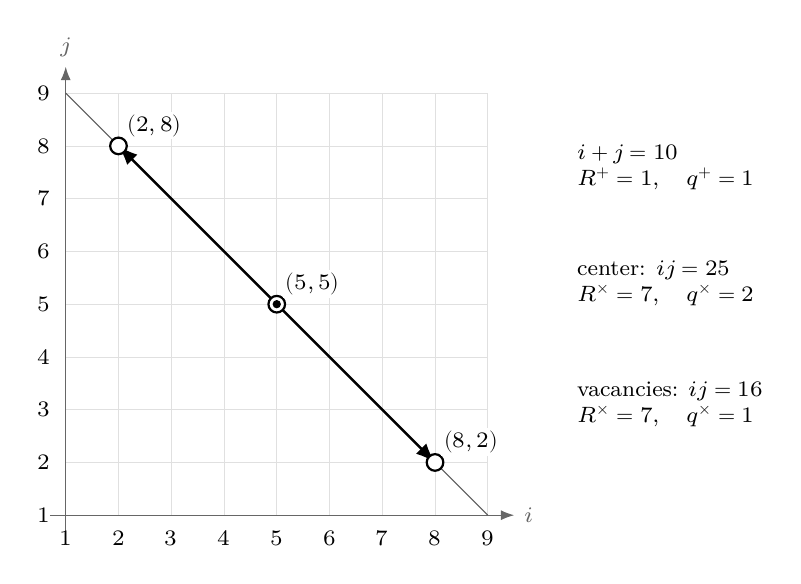
\begin{tikzpicture}[x=.67cm,y=.67cm,font=\footnotesize,>=Latex]
 \draw[step=1,black!12,line width=.3pt] (1,1) grid (9,9);
 \draw[->,black!60] (.7,1)--(9.5,1) node[right] {$i$};
 \draw[->,black!60] (1,.7)--(1,9.5) node[above] {$j$};
 \foreach \k in {1,...,9}{
  \node[below=2pt] at (\k,1) {$\k$};
  \node[left=2pt] at (1,\k) {$\k$};
 }
 \draw[black!65] (1,9)--(9,1);
 \draw[<->,line width=.9pt] (2,8)--(8,2);
 \foreach \x/\y in {2/8,5/5,8/2}{
  \filldraw[fill=white,line width=.8pt] (\x,\y) circle (3pt);
 }
 \fill (5,5) circle (1.5pt);
 \node[above right=3pt,fill=white,inner sep=1pt] at (2,8) {$(2,8)$};
 \node[above right=3pt,fill=white,inner sep=1pt] at (5,5) {$(5,5)$};
 \node[above right=3pt,fill=white,inner sep=1pt] at (8,2) {$(8,2)$};
 \node[anchor=west,align=left] at (10.5,7.6)
   {$i+j=10$\\$R^+=1,\quad q^+=1$};
 \node[anchor=west,align=left] at (10.5,5.4)
   {center: $ij=25$\\$R^\times=7,\quad q^\times=2$};
 \node[anchor=west,align=left] at (10.5,3.1)
   {vacancies: $ij=16$\\$R^\times=7,\quad q^\times=1$};
\end{tikzpicture}
\caption{Electronic center and conjugate vacancies in the APP chart.
The diagonal is the additive fiber \(\mathcal F_{10}\); the center
is the fixed point of \((i,j)\mapsto(10-i,10-j)\). The two
shifts of magnitude \(3\) preserve the sum and product
residue and reduce the multiplicative quotient by one unit. The
arrows represent deformations on the fiber.}
\label{el-centro:figura}
\end{figure}


Central symmetry also characterizes its persistence under changes of
chart. If an admissible atlas transformation \(f\) intertwines
inversion, \(f\rho=\rho f\), then
\[
 \rho f(5,5)=f\rho(5,5)=f(5,5).
\]
Uniqueness of the fixed point forces \(f(5,5)=(5,5)\). This is the
internal property making the central location stable: every
transformation of that type preserves the cell before evaluating its
electronic character.

The central matrix block belongs to evaluation on the two
adjacent positions \(4,5\). Its decomposition, established in the
local development of the kernel, is
\[
 B_c=\begin{pmatrix}7&2\\2&7\end{pmatrix}=9P_++5P_-.
\]
Here \(9\) and \(5\) are eigenvalues of two modes, whereas
\((5,5)\) is a position in the atlas. Concatenations of its
entries give \(72+27=77+22=99\) and
\(77-22=55=54+1\). The first equality preserves the total sum under
two arrangements; the second expresses the defect between diagonal
and antidiagonal readings. These operations precede electronic
composition and preserve their matrix provenance.

The initial orientation is another datum. In the representation of
electronic return, \((h_0,v_0)=(1,1)\) is fixed, that is, positive
advance in both coordinates. Simultaneous inversion every \(27\)
steps, read in windows of \(9\), determines
\[
 \tau_e=(+1,+1,+1,-1,-1,-1,+1,+1,+1,-1,-1,-1).
\]
The segments \((1,1,1)\) belong to this orientation sequence:
each segment comprises three windows in the same direction. The recurrence
in the section on readers proves this record in
\eqref{eq:el-tau}, and its two evaluations recover the triple
\((80,54,6)\) entering
\eqref{eq:el-formula-completa}. The positional coordinate,
APP quotients, and sign sequence are thus connected through
explicit operations.

The signature \(555555\) belongs to a regional reading in another
domain. For a decimal emission \(U=(U_1,\ldots,U_6)\), we write
\(U_j=100d_{1j}+10d_{2j}+d_{3j}\), with three digits, including
leading zeros. The multiplicative-signature reader is
\[
 \mathcal E_\times(U)
   =\bigl([d_{2j}-d_{1j}]_{10}\bigr)_{j=1}^{6}.
\]
In the transversal region
\(U_\pi^\perp=(501,614,498,169,272,272)\), the differences are
\((-5,-5,5,5,5,5)\). Consequently,
\begin{equation}
 \mathcal E_\times(U_\pi^\perp)=(5,5,5,5,5,5),\qquad
 \Psi(U_\pi^\perp)=010211.
 \label{el-centro:firma-transversal}
\end{equation}
The first map preserves a multiplicative signature of the catalog;
the second preserves the ternary word common to the five regions.
Figure \ref{pi-estrella:figura} shows the transversal position of
this emission and its multiplicity \(432\).

\paragraph{Memory required to transport the constant signature.}
The signature \(555555\) additionally provides a verifiable example of
the trajectory information required by TPK. Let
\(\mathcal X_\times=D_9^2\times\{N,E,S,O\}\), with \(324\)
oriented positions in the product channel. Advance \(P\) moves
one square in the stored direction, and the half-turn \(H\)
reverses that direction. In this representation, the reader
\(E_{\rm sig}\) sums the discrete exponents by windows:
\[
 \ell_9(1,2,4,8,7,5)=(0,1,2,3,4,5),\qquad
 \ell_9(3)=\ell_9(6)=\ell_9(9)=0.
\]
During each of the six nine-step windows,
\(\ell_9(\rho_9(ij))\) is evaluated before every product advance, selected
by TRIT at times \(2,5,8\pmod9\). The window sum is
reduced modulo \(10\). After steps \(27\) and \(54\), the
direction is reversed. This rule determines the six components of
\(E_{\rm sig}\) from the initial position and orientation.

Enumeration of this domain produces \(26\) signatures. The fiber of
\(555555\) contains \(24\) oriented positions; after one
advance, their images are distributed among three signatures, with eight
representatives each:
\[
 555177,\qquad555717,\qquad555771.
\]
Three witnesses, in coordinates from \(1\) to \(9\), allow the
distinction to be checked directly:
\[
\begin{array}{c|c|c}
x&E_{\rm sig}(x)&E_{\rm sig}(Px)\\\hline
(3,5,N)&555555&555177\\
(3,4,N)&555555&555717\\
(3,4,S)&555555&555771
\end{array}
\]
Thus, the common value of the signature does not determine its next value:
the transport class within that fiber forms part of the operational
datum. The minimal stable partition is calculated by starting from
signature equivalence \(\sim_0\) and refining through
\[
 x\sim_{n+1}y\quad\Longleftrightarrow\quad
 x\sim_n y,\quad Px\sim_n Py,\quad Hx\sim_n Hy.
\]
The procedure terminates because the domain is finite. Every stable
congruence refining \(\sim_0\) refines every \(\sim_n\), by induction;
its fixed point is therefore the minimal stable congruence required.
The census gives \(26\to28\to28\), with histogram
\(27\cdot8+108=324\). The only signature that splits is
\(555555\), into three classes of eight elements. The accompanying certificate
reproduces the enumeration, the three classes, and stability under both
operators.

The multiplicity \(24\) here belongs to the product-channel fiber;
the multiplicity \(432\) belongs to the complete regional emission
\(U_\pi^\perp\). The first proves why the signature needs transport
memory; the second places that signature within the joint catalog of
the two sheets. Both readings participate in the same architecture,
with specified domains and operations.

This distinction of domains makes it possible to bring together the occurrences of unity
and the center with their respective meanings:
\begin{center}
\small
\begin{tabularx}{\textwidth}{@{}lX@{}}
\toprule
Record & Object and function \\
\midrule
\((5,5)\) & Fixed cell of the central inversion of the APP atlas.\\
\((R^+,q^+)=(1,1)\) & Residue and quotient of the central additive evaluation.\\
\((h_0,v_0)=(1,1)\) & Initial orientation of the two shifts.\\
\((+1,+1,+1)\) & Three consecutive windows of \(\tau_e\) with positive orientation.\\
\(c=111111\) & Datum of the fifth nonadic boundary, Section \ref{mono-recta:desarrollo}.\\
\(\mathcal E_\times=555555\) & Signature of the transversal region of \(\pi\), with six positions.\\
\bottomrule
\end{tabularx}
\end{center}

Electronic coordination is obtained by composing these levels in their
dependency order. APP determines the center and evaluations;
TRIT selects regimes and orientations; TPK prolongs the trajectory
and preserves its records. The previously generated regions provide
the characters \(\pi,\varphi,e\); the dodecaphase record provides
\(\alpha\); the electronic readers determine the factors of
equation \eqref{eq:el-formula-completa}. This composition preserves
the identity of the section throughout its different
representations, up to dimensional evaluation and subsequent
metrological comparison.


\subsection{Commutator norm of the arithmetic projections}

The electronic prefactor is obtained without using \(\alpha\), torsion,
or a dimensional unit. The domain is the third realization of APP,
\(\mathcal A_3=\{1,\ldots,9\}^3\), equipped with the uniform measure.
We define
\[
 \Sigma(x)=\rho_9(x_1+x_2+x_3),\qquad
 \Pi(x)=\rho_9(x_1x_2x_3).
\]
The conditional expectations \(P_\Sigma\) and \(P_\Pi\) are the
orthogonal projections onto functions constant on each additive
and multiplicative fiber, respectively. Thus, for a function \(f\),
\[
 (P_\Sigma f)(x)
 =\frac{1}{|\Sigma^{-1}(\Sigma(x))|}
   \sum_{y:\,\Sigma(y)=\Sigma(x)}f(y),
\]
and analogously for \(P_\Pi\). The two projections act on the
same space; they do not represent two independent arithmetic supports.

\begin{lemma}[Two projections and principal angles]
If \(s\in[0,1]\) is a singular value of the pairing between
orthonormal bases of the ranges of two projections \(P,Q\), its nontrivial
block contributes \(s\sqrt{1-s^2}\) to
\(\|[P,Q]\|\).
\end{lemma}
\begin{proof}
On the corresponding principal plane, one can write
\[
 P=\begin{pmatrix}1&0\\0&0\end{pmatrix},\qquad
 Q=\begin{pmatrix}
 s^2&s\sqrt{1-s^2}\\
 s\sqrt{1-s^2}&1-s^2
 \end{pmatrix}.
\]
Their commutator is
\[
 [P,Q]=s\sqrt{1-s^2}
 \begin{pmatrix}0&1\\-1&0\end{pmatrix}.
\]
The final matrix is orthogonal, so its norm is one. Common
or orthogonal blocks have zero commutator. The orthogonal decomposition
into principal planes gives the claim and reduces the total norm to the maximum
of these contributions.
\end{proof}

\begin{proposition}[Exact incompatibility norm]
On \(\ell^2(\mathcal A_3)\),
\begin{equation}
 \|[P_\Sigma,P_\Pi]\|=\frac{\sqrt3}{4}.
 \label{eq:el-prefactor}
\end{equation}
\end{proposition}
\begin{proof}
Let \(N_{ab}=|\Sigma^{-1}(a)\cap\Pi^{-1}(b)|\). Integer enumeration
of the three symbols yields
\[
 N=9\begin{pmatrix}
 0&1&1&0&1&1&0&1&4\\
 1&0&1&1&0&1&1&0&4\\
 1&0&2&0&1&2&0&0&3\\
 0&1&1&0&1&1&0&1&4\\
 1&0&1&1&0&1&1&0&4\\
 0&0&2&1&0&2&0&1&3\\
 0&1&1&0&1&1&0&1&4\\
 1&0&1&1&0&1&1&0&4\\
 0&1&2&0&0&2&1&0&3
 \end{pmatrix}.
\]
Each row sums to \(81\); the column sums are
\[
 (m_1,\ldots,m_9)=(36,36,108,36,36,108,36,36,297).
\]
The normalized indicator functions of the fibers have pairing
matrix \(C_{ab}=N_{ab}/\sqrt{81m_b}\). Consequently,
\[
 M=CC^{\mathsf T},\qquad
 M_{ac}=\sum_{b=1}^9\frac{N_{ab}N_{cb}}{81m_b}
\]
is a rational matrix whose spectrum consists of the squares of the
required singular values.

Exact multiplication shows that \((1,\ldots,1)\),
\((1,-1,0)^3\), and \((1,1,-2)^3\) are eigenvectors with eigenvalues
\(1\), \(1/4\), and \(7/132\), respectively. The subspace of
vectors supported on \(\{3,6,9\}\) whose sum is zero has dimension
two and eigenvalue \(1/18\). The zero-sum vectors supported on
\(\{1,4,7\}\) or \(\{2,5,8\}\) form a four-dimensional
kernel. These subspaces are independent and their dimensions sum to
nine. The complete spectrum is therefore established:
\[
 \operatorname{spec}(M)=
 \left\{1,\frac14,\frac7{132},\frac1{18},\frac1{18},0,0,0,0\right\}.
\]
The maximum of \(\lambda(1-\lambda)\) on this set is \(3/16\),
attained at \(\lambda=1/4\). The preceding lemma gives
\(\sqrt{3/16}=\sqrt3/4\).
\end{proof}

The mode \((1,-1,0)^3\) is precisely the distribution of values of the
tritic phase selector in the nonadic chart. The scalar norm retains
a measure of incompatibility, but does not by itself preserve the
orientation of that mode or reconstruct the two projectors. That memory
remains in the route state accompanying the scalar reading.

\begin{proposition}[Algebra of the local electronic block]
On the principal plane attaining \eqref{eq:el-prefactor}, let
\[
 P=\begin{pmatrix}1&0\\0&0\end{pmatrix},\qquad
 Q=\begin{pmatrix}1/4&\sqrt3/4\\\sqrt3/4&3/4\end{pmatrix},\qquad
 S=2P-I,\qquad J=\frac4{\sqrt3}[P,Q].
\]
Then \(S^2=I\), \(J^2=-I\), \(SJ=-JS\), and the real algebra
generated by \(S,J\) is \(M_2(\mathbb R)\), a realization of
\(\mathrm{Cl}_{1,1}\). Moreover,
\[
 n_\pm=\frac{S\pm J}{2},\qquad
 n_\pm^2=0,\qquad n_+n_-+n_-n_+=I.
\]
\end{proposition}
\begin{proof}
We have \(S=\operatorname{diag}(1,-1)\) and
\(J=\bigl(\begin{smallmatrix}0&1\\-1&0\end{smallmatrix}\bigr)\).
Multiplication verifies the three relations. The matrices
\(I,S,J,SJ\) are linearly independent and form a basis of
\(M_2(\mathbb R)\), proving the claim about the algebra.
Finally, \((S\pm J)^2=S^2+J^2\pm(SJ+JS)=0\), and the sum of the
cross products is \((S^2-J^2)/2=I\).
\end{proof}

In this block, an elliptic direction, a hyperbolic direction, and two
parabolic null directions coexist. The result describes a local
matrix representation of the arithmetic of the two sheets. It does not identify all of APP
with \(M_2(\mathbb R)\), or with a quantum Latin square; such
claims would require other domains and other relations. Nor does the
exponential belong exclusively to the parabolic regime: it can
be applied to any of the generators of this block.

% Proposed focal addition; does not replace the existing electronic algebra.
% Insertion: after the proposition "Algebra of the local electronic block"
% and its explanatory paragraph, before "Transfer between sheets...".
% Provenance and scope: LOCALIZADORES_Y_ALCANCE.md, in this folder.
\subsection{Spinor representation of the electronic block and helicity}
\label{sec:el-representacion-espinorial}

The electronic structure has a representation preserving more
information than its scalar evaluation. The principal plane of the two
three-dimensional APP projectors, selected by the tritic mode
\((1,-1,0)^3\), has already provided the operators \(S\) and \(J\).
The former is a symmetric involution; the latter is the normalized
commutator and preserves sheet orientation. Their composition makes it possible
to construct explicitly a rotation representation and separate its
two helicity components. This construction acts on the electronic
block; the TPK route record and its memory remain as data
of the block's provenance.

Let \(E_e\) be the real principal plane, equipped with the inner product inherited
from the conditional expectations, and let
\(\mathscr S_e=E_e\otimes_{\mathbb R}\mathbb C\) be its complexification.
The operators already obtained satisfy
\[
 S^*=S,\qquad J^*=-J,\qquad
 S^2=I,\qquad J^2=-I,\qquad SJ=-JS.
\]
Complexification extends the representation field. It preserves the
real operators and allows the scalar unit \(i\) to be distinguished from the
endomorphism \(J\), although both square to \(-1\) in their
respective domains.

\begin{proposition}[Hermitian triple induced by the two sheets]
\label{prop:el-terna-hermitica}
The operators
\begin{equation}
 \sigma_1=SJ,\qquad \sigma_2=-iJ,\qquad \sigma_3=S
 \label{eq:el-terna-hermitica}
\end{equation}
are Hermitian and traceless. They satisfy
\begin{equation}
 \sigma_a\sigma_b
 =\delta_{ab}I+i\sum_{c=1}^3\epsilon_{abc}\sigma_c,
 \qquad
 \frac12\operatorname{tr}(\sigma_a\sigma_b)=\delta_{ab},
 \label{eq:el-algebra-terna}
\end{equation}
where \(\epsilon_{123}=1\). They therefore form an orthonormal basis
of the real space \(V_e\) of traceless Hermitian endomorphisms of
\(\mathscr S_e\), for the inner product
\(\langle X,Y\rangle=\frac12\operatorname{tr}(XY)\).
\end{proposition}
\begin{proof}
The preceding relations give \((SJ)^*=(-J)S=SJ\) and
\((-iJ)^*=-iJ\). The squares of all three matrices are \(I\).
Furthermore,
\[
 (SJ)(-iJ)=iS,\qquad (-iJ)S=iSJ,\qquad S(SJ)=J=i(-iJ).
\]
Reversing the order changes the sign. This proves the first identity
in \eqref{eq:el-algebra-terna}. In the orthonormal basis of the principal plane,
the matrices are
\[
 \sigma_1=\begin{pmatrix}0&1\\1&0\end{pmatrix},\quad
 \sigma_2=\begin{pmatrix}0&-i\\i&0\end{pmatrix},\quad
 \sigma_3=\begin{pmatrix}1&0\\0&-1\end{pmatrix}.
\]
Their trace is zero, and taking traces in the product identity proves
orthonormality. Every traceless Hermitian endomorphism has the form
\(\bigl(\begin{smallmatrix}z&x-iy\\x+iy&-z\end{smallmatrix}\bigr)\),
with real \(x,y,z\), and thus belongs to their real span.
\end{proof}

In the usual matrix representation, this triple is called the
Pauli matrices. Their use here follows the construction of
\(P,Q,S,J\): they are obtained through the products
\eqref{eq:el-terna-hermitica}. The direction space of this
representation is the unit sphere of \(V_e\), whose positive form
has just been constructed through the trace.

\begin{proposition}[Rotation generators and directional decomposition]
\label{prop:el-helicidad}
Define \(L_a=\sigma_a/2\). Then
\begin{equation}
 [L_a,L_b]=i\sum_c\epsilon_{abc}L_c,
 \qquad \sum_{a=1}^3L_a^2=\frac34 I.
 \label{eq:el-generadores-spin}
\end{equation}
For \(n=(n_1,n_2,n_3)\) with \(\sum_an_a^2=1\), let
\[
 H_e(n)=\sum_an_a\sigma_a,\qquad
 h_e(n)=\frac12H_e(n),\qquad
 \Pi_\pm(n)=\frac12\bigl(I\pm H_e(n)\bigr).
\]
The linear formula \(H_e(v)=\sum_av_a\sigma_a\) is also used
for \(v\) of arbitrary norm.
One has
\begin{equation}
 \mathscr S_e=\operatorname{im}\Pi_+(n)
             \mathbin{\oplus}\operatorname{im}\Pi_-(n),
 \qquad
 h_e(n)\Pi_\pm(n)=\pm\frac12\Pi_\pm(n).
 \label{eq:el-descomposicion-helicidad}
\end{equation}
The two summands are orthogonal complex lines. Rotation
transport around \(n\) is
\begin{equation}
 U_n(\theta)=\exp\!\left(-\frac{i\theta}{2}H_e(n)\right)
 =\cos\frac\theta2\,I-i\sin\frac\theta2\,H_e(n),
 \qquad
 U_n(2\pi)=-I,\quad U_n(4\pi)=I.
 \label{eq:el-retorno-spin}
\end{equation}
\end{proposition}
\begin{proof}
The product identity of the triple gives the commutators in
\eqref{eq:el-generadores-spin}; their squares sum to \(3I/4\).
Antisymmetric terms cancel when multiplying
\(H_e(n)\) by itself, so that \(H_e(n)^2=I\).
It follows that
\[
 \Pi_\pm(n)^2=\Pi_\pm(n),\qquad
 \Pi_+(n)\Pi_-(n)=0,\qquad \Pi_+(n)+\Pi_-(n)=I.
\]
They are Hermitian and have trace \(1\); their rank is therefore \(1\).
Multiplication by \(H_e(n)/2\) proves
\eqref{eq:el-descomposicion-helicidad}. The exponential series
splits into even and odd powers because \(H_e(n)^2=I\), producing
\eqref{eq:el-retorno-spin}. It also directly proves
unitarity and the law \(U_n(\theta+\psi)=U_n(\theta)U_n(\psi)\).

Angular normalization is verified on \(V_e\). For every
\(v\in\mathbb R^3\), the same product identity gives
\[
 U_n(\theta)H_e(v)U_n(\theta)^*
 =H_e\!\left(v\cos\theta+(n\mathbin{\times}v)\sin\theta
       +n(n\mathbin{\cdot}v)(1-\cos\theta)\right).
\]
The induced action is a rotation of angle \(\theta\) and axis \(n\).
The factor \(1/2\) in the spinor generator is therefore the one
corresponding to that angular parameterization. A complete rotation restores
the direction in \(V_e\) and changes the sign of the vector in
\(\mathscr S_e\); two complete rotations restore both.
\end{proof}

The representation is irreducible: a complex subspace invariant under
the three matrices would be invariant under all of \(M_2(\mathbb C)\), the
algebra they generate. Its only invariant subspaces are \(0\) and
\(\mathscr S_e\). The relations
\eqref{eq:el-generadores-spin} thus identify the spin-\(1/2\)
representation. If \(n\) is the propagation direction in a
kinematic realization, \(h_e(n)\) is its dimensionless helicity, with
values \(\pm1/2\). The kinematic direction is declared when that
realization is made; the two projectors are defined for every direction
before a particular propagation state is selected.

\paragraph{Preservation of the electronic structure and types of inversion.}
Direction inversion has an exact law:
\[
 H_e(-n)=-H_e(n),\qquad \Pi_\pm(-n)=\Pi_\mp(n).
\]
This operation exchanges helicity labels relative to a
direction. Charge conjugation, by contrast, acts on the oriented
signature of the material route; cellular inversion acts on the
atlas coordinates. Their domains and actions remain distinct.
Uniqueness of cell \((5,5)\) is compatible with the two lines in
\eqref{eq:el-descomposicion-helicidad}: an atlas cell is not a
vector in the spinor representation it carries.

The electronic evaluation \(\varepsilon_e^\beta\) preserves its
formula and readers. On \(\mathscr S_e\), its scalar realization
is \(\varepsilon_e^\beta I\), which commutes with the generators and with
\(\Pi_\pm(n)\). Helicity decomposition adds rotational
information without modifying the evaluation or turning spin into a
multiplicative mass coefficient.

Chirality corresponds to the grading of the relativistic representation
used: an involution \(\Gamma_{\rm ch}\) determines its
projectors \((I\mp\Gamma_{\rm ch})/2\). The helicity in
\eqref{eq:el-descomposicion-helicidad} additionally depends on \(n\).
For its part, the holonomy of a real Möbius band describes the change
of sign of a line when traversing a loop in its base. The law of that line,
the spinor return \eqref{eq:el-retorno-spin}, and nonadic phase holonomy
with memory advance are transport laws on specified
objects. Their comparison preserves those objects: the helical form
of a trajectory does not replace the representation just
constructed or by itself fix chirality or charge.


\subsection{Transfer between sheets and coefficients of the basal stage}

The primitive tritic calendar visits the modes
\((\Sigma,\Pi,\Pi)\). Counting consecutive pairs, including the
closure of the block, yields one transition \(\Sigma\to\Pi\), one
\(\Pi\to\Pi\), and one \(\Pi\to\Sigma\). Their primitive incidence is
\[
 F_{\mathrm{av}}=\begin{pmatrix}0&1\\1&1\end{pmatrix}.
\]
This matrix realization is obtained after the calendar. It is not
used to replace the coinductive reader that has already generated \(\varphi\).
Its characteristic polynomial is \(X^2-X-1\), and recognition of the
two roots as \(\varphi\) and \(-\varphi^{-1}\) describes the action of
that output in modal transfer. The quadratic action has eigenvalues
\(\varphi^2,-1,\varphi^{-2}\); the last is the positive stable mode.
The regional mark \(\pi\), applied once, gives
\(\pi/\varphi^2\).

The trajectory space, its measure, and the closure operator are
constructed in subsections~\ref{sec:medida-retorno-hojas}
and~\ref{sec:operador-retorno-marcado}. Formula
\eqref{eq:retorno-marcado-finito} preserves its provenance as a quotient
of returns; the electronic application subsequently composes this reading
with the following involution. The regional signature \(555555\) accompanies
the closure region, whose transport preserves the state with memory;
the centre \((5,5)\) fixes the cell of origin of the oriented electronic
section. Both kinds of information converge in the composition and retain
their respective domains.

\begin{lemma}[Interchange of the two orientations]
Let \(\mathcal R(x,y)=x/y^2\) and
\(\mathscr S_{\pi\varphi}(x,y)=(y,x)\), for \(x,y>0\).
Then
\begin{equation}
 \begin{aligned}
 \mathscr S_{\pi\varphi}^{\,2}&=I,\qquad
 \mathcal R(\pi,\varphi)=\frac{\pi}{\varphi^2},\\
 (\mathcal R\circ\mathscr S_{\pi\varphi})(\pi,\varphi)
 &=\frac{\varphi}{\pi^2}
 =\frac1{\varphi^3(\pi/\varphi^2)^2}.
 \end{aligned}
 \label{eq:el-bisagra}
\end{equation}
\end{lemma}
\begin{proof}
Applying the interchange twice gives the identity. Moreover,
\(\varphi^3(\pi/\varphi^2)^2=\pi^2/\varphi\); taking its inverse proves
the last equality.
\end{proof}

The electronic reader uses the orientation \(\varphi/\pi^2\),
followed by the exponential character. The preceding identity explains the
interchange, but does not replace the rule that chooses that character or
by itself produce the integers of the correction. These have a different provenance.

The phase-compatible central return has minimal length
twenty-seven. With the phase and sheet record, its finite space is
\[
 \mathcal K_e=\mathbb Z/9\mathbb Z\times\mathbb F_3.
\]
The five regions of \(\pi\) are distinct genealogical identities,
not five interchangeable copies of a visible expansion. In the regional
gauge fixed by the construction, their injection into the return occupies
the positions
\begin{equation}
 (4,0),\quad(5,0),\quad(6,0),\quad(6,1),\quad(6,2).
 \label{eq:el-cinco-lugares}
\end{equation}
The transverse orientation, mutated return, and three positive
regions remain separated by that record. Admissible changes
of gauge transport the labels jointly; they do not reselect
the positions from an electronic value.

\begin{proposition}[Deficit and retained memory]
Given the central return and the preceding regional injection, the oriented
boundary deficit and torsional memory are
\begin{equation}
 n_e=-|\mathcal K_e\setminus\iota(\mathscr R_\pi)|=-22,
 \qquad
 m_e^{\mathrm{tor}}=|\mathscr R_\pi\times\mathbb F_3|=15.
 \label{eq:el-selector-enteros}
\end{equation}
\end{proposition}
\begin{proof}
The five positions in \eqref{eq:el-cinco-lugares} are distinct.
Thus, \(|\mathcal K_e|=9\cdot3=27\), and the complement of the image
has cardinality \(27-5=22\). The orientation convention records
the deficit removed from the boundary as negative. The retained memory has
three sheets per region, so its positive cardinality is
\(5\cdot3=15\).
\end{proof}

The same pair has the integer check supplied by the collection's APP chart:
\begin{equation}
 396=18+72+108+198,
 \qquad \frac{396}{18}=22,
 \qquad \frac{270}{18}=15=3\cdot5=\binom62.
 \label{eq:el-censo}
\end{equation}
The weight \(18\) belongs to the central \(2\times2\) kernel, and \(270\)
to the declared global channel. These equalities check the normalization
of the count; the return argument also fixes the signs. The
quotient of the alternating rings,
\(396/(18+108)=22/7\), is rational and is not identified with \(\pi\).
Nor does \(\binom62\) mean \(6/2\): it counts the unordered pairs
of a six-element set.

Evaluation of the deficit in the third symmetric realization uses
\(\alpha^3\). This power is the product of three copies of the
closure scalar already obtained; it does not assert a universal rule
associating any dimension with the same power of \(\alpha\).
The specified domain and reader are essential to the composition.

\subsection{Global torsion and the basal coordinate}

\begin{definition}[Electronic torsional normalization]
The reduced defect \(d_4\) and the complete reader
\(\Delta_4\) are distinguished:
\begin{equation}
 d_4=\frac{\pi-e\log\pi}{270},\qquad
 \Delta_4=d_4\left(1+\frac{\pi}{729}\right).
 \label{eq:el-delta}
\end{equation}
The denominator \(270\) corresponds to the census channel, whereas the
factor \(1+\pi/729\) retains the coupling with the cubic cell of
\(729\) positions. The electronic reading uses \(\Delta_4\) both in
its basal stage and in the return exponent.
\end{definition}

This definition acts on previously generated \(\pi\) and \(e\). The
logarithm is a subsequent operation in their real realization, not a
retrospective input of conventional values. Torsion is global:
it is not determined independently for each section by an observed
mass.

\begin{lemma}[The two normalizations are not interchangeable]
We have
\begin{equation}
 \Delta_4-d_4=\frac{\pi}{729}d_4.
 \label{eq:el-delta-diferencia}
\end{equation}
In particular, \(d_4>0\) and \(\Delta_4>d_4\) for the coordinates
under consideration.
\end{lemma}
\begin{proof}
The identity follows by distributivity. For positivity, the function
\(f(x)=x-e\log x\), on \(x>0\), has derivative \(1-e/x\) and
second derivative \(e/x^2>0\). Its unique minimum is at \(x=e\), where
it is zero. Since \(\pi\ne e\), we have \(f(\pi)>0\). Both factors
in \eqref{eq:el-delta} are positive and \(1+\pi/729>1\).
\end{proof}

\begin{remark}[Preservation of the normalization]
Removing the second factor in \eqref{eq:el-delta} changes the reader; it
is not an algebraic simplification. If \(d_4\) is introduced as an
auxiliary coordinate, the same object must be written as
\(\Delta_4=(1+\pi/729)d_4\) in every occurrence. Keeping the
integers \(15\) and \(6\) and replacing only \(\Delta_4\) by \(d_4\)
produces a different formula.
\end{remark}

\begin{definition}[Basal electronic coordinate]
The composition of incompatibility, modal transfer, deficit, and retained memory
is
\begin{equation}
 \varepsilon_e^{(0)}
 =\frac{\sqrt3}{4}
  \left[\exp\!\left(\frac{\varphi}{\pi^2}\right)-22\alpha^3\right]
  (1+15\Delta_4).
 \label{eq:el-basal}
\end{equation}
\end{definition}

The equation combines three operations of different kinds. The norm
\(\sqrt3/4\) quantifies the incompatibility of the sheet
projections; its origin is a principal angle of the APP fibers.
The exponential acts on the orientation \(\varphi/\pi^2\) of the
transfer reader. The cubic subtraction records the \(22\) complementary
positions of the marked return, and the torsional factor preserves the
\(15\) components corresponding to three sheets per region. The
composition preserves these domains even though its final evaluation is scalar.

The presence of \(\pi\), \(\varphi\), and \(e\) thus has operational
meanings. Euler's number enters through the exponential and
the logarithmic normalization of \(\Delta_4\); \(\varphi\) and \(\pi\)
enter through oriented transfer. The constant \(\alpha\)
acts after its own construction through the cubic closure
term. The chronological return must still act on this basal
coordinate. Separating the stages makes it possible to explain what changes when
an orientation, normalization, or record is modified, while preserving the central
structure that identifies the electronic section.

The parentheses in this equation are part of its content. The term
\(-22\alpha^3\) is subtracted \emph{outside} the exponential; the memory
\(1+15\Delta_4\) multiplies the entire bracket. Placing the deficit in
the exponent or applying a different torsion to it would alter the composition.

\begin{proposition}[Basal positivity]
For \(0<\alpha<10^{-2}\), \(\varphi>0\), and the normalization
\eqref{eq:el-delta}, we have \(\varepsilon_e^{(0)}>0\).
\end{proposition}
\begin{proof}
The exponential is greater than one, and
\(22\alpha^3<22\cdot10^{-6}<1\). The bracket is therefore positive.
Also, \(1+15\Delta_4>1\) and \(\sqrt3/4>0\).
\end{proof}

The subsequent evaluation of \eqref{eq:el-basal} begins with
\[
 \varepsilon_e^{(0)}=0.5109989224880660725\ldots.
\]
This number is still a dimensionless coordinate and is not the
final stage: the return memory of the route itself remains to be applied.

\subsection{Determinantal action scale and decimal valuation}

The absolute scale and the relative corrector originate in different
objects. The former uses the local block of the step-three dodecaphasic
record,
\begin{equation}
 H_4=\begin{pmatrix}
 1&1&1&1\\1&1&-1&-1\\1&-1&1&-1\\1&-1&-1&1
 \end{pmatrix},\qquad
 G_H=\mathbb Z^4/H_4\mathbb Z^4.
 \label{eq:el-h4}
\end{equation}
The operation uses a local quotient. The three blocks of the complete
record are not replaced by a tensorization that would multiply
the number of sheets of this reader again.

\begin{lemma}[Number of sheets of the local quotient]
The Smith normal form of \(H_4\) is
\(\operatorname{diag}(1,2,2,4)\). Consequently,
\[
 G_H\simeq\mathbb Z/2\mathbb Z\oplus\mathbb Z/2\mathbb Z
 \oplus\mathbb Z/4\mathbb Z,\qquad |G_H|=16.
\]
\end{lemma}
\begin{proof}
The greatest common divisor of the entries is one. The order-two minors
are even, and one has value \(-2\), so their greatest common divisor
is two. Since \(H_4H_4^{\mathsf T}=4I\) and \(\det H_4=-16\), the
cofactors are \(\pm4\); the third determinantal divisor is four.
The fourth is \(16\). The successive quotients of the divisors
\(1,2,4,16\) are \(1,2,2,4\). Their product gives the order of the quotient.
\end{proof}

\begin{definition}[Determinantal action reader]
The multiplicative norm of the scalar section \(\alpha\), constant
over the sheets of \(G_H\), and one application of self-scaling
\(\varphi\) produce
\begin{equation}
 \Sigma_H=\varphi\,\mathrm N_{G_H}(\alpha),\qquad
 \mathrm N_{G_H}(\alpha)=\prod_{g\in G_H}\alpha=\alpha^{16}.
 \label{eq:el-lector-determinantal}
\end{equation}
The associated decimal chart determines
\(\operatorname{ord}_{10}(\Sigma_H)=\lfloor\log_{10}\Sigma_H\rfloor\).
\end{definition}

The sixteenth power thus comes from the number of sheets of the quotient,
once this local reader is fixed. The factor \(\varphi\) acts once on
the basis of the action line. Smith computation alone would not
select every possible functional on the quotient: the multiplicative
norm and self-scaling form part of the stated operation.

\begin{theorem}[Decade of the action section]
The reader \eqref{eq:el-lector-determinantal}, applied to the already
generated HMT coordinates, satisfies
\begin{equation}
 10^{-34}<\Sigma_H<10^{-33},\qquad
 \operatorname{ord}_{10}(\Sigma_H)=-34.
 \label{eq:el-decada}
\end{equation}
\end{theorem}
\begin{proof}
The following rational intervals, much coarser than the available
cylinders, suffice:
\[
 \frac{1618}{1000}<\varphi<\frac{1619}{1000},\qquad
 \frac{7297}{10^6}<\alpha<\frac{7298}{10^6}.
\]
The function \((x,a)\mapsto xa^{16}\) is increasing in both positive
arguments. The two integer inequalities
\[
 1618\cdot7297^{16}>10^{65},\qquad
 1619\cdot7298^{16}<10^{66}
\]
imply
\[
 10^{-34}
 <\frac{1618}{1000}\left(\frac{7297}{10^6}\right)^{16}
 <\Sigma_H
 <\frac{1619}{1000}\left(\frac{7298}{10^6}\right)^{16}
 <10^{-33}.
\]
The definition of decimal order concludes the proof. Neither an
SI unit nor a reference mass participates in these inequalities.
\end{proof}

The normalized section begins with
\(\Sigma_H=1.0462438381\ldots\times10^{-34}\). Its mantissa is not
identified with the action coordinate before or after return.
The determinantal reader fixes the decimal order; the two return
coordinates are obtained through the following readers.

\subsection{Action sections and dimensionless return quotient}

Let \(\mathcal L_S\) be an oriented action line and \(\mathcal U_S\)
its positive basis. The electronic composition uses two sections of
this line and their dimensionless quotient. Its construction requires
the determinantal decade already obtained, the fifth-order action character,
and the regional contribution of the return.

\subsubsection{Action character and provenance of its coefficients}
\label{sec:revision-planck}

The reduced Planck constant, \(\hbar\), is the physical object
motivating the realization of the angular action section. Its place in
the electronic dependency must be specified at two levels. The
determinantal norm \(\Sigma_H\) determines the decade of the scale. The
character \(H_5\) and regional return then determine the coordinates
of the action sections. This separation allows the result required
for the electron to be presented without anticipating the complete developments
of other sectors of dimensional mechanics.

The provenance of the fifth-order character can be made explicit through
invariants already fixed on the support. In the central chart, consider
\[
 B_c=\begin{pmatrix}7&2\\2&7\end{pmatrix},
 \qquad \lambda_+=9,\quad\lambda_-=5.
\]
The calendar has length \(12\), the orbit of step \(3\) has
length \(4\), and the relevant count quotient is
\(104976/1944=54\). The character coefficients satisfy
\begin{equation}
 \frac9{16}=\frac{\lambda_+}{4^2},\quad
 \frac59=\frac{\lambda_-}{\lambda_+},\quad
 \frac7{48}=\frac{\operatorname{tr}(B_c)/2}{4\cdot12},\quad
 \frac1{54}=\frac{1944}{104976}.
 \label{eq:revision-h5-coeficientes}
\end{equation}
The assignment of these invariants to degrees \(2,3,4,5\), with the
alternating signs in \eqref{eq:el-h5}, belongs to the definition of the
analytic character used. Making it explicit is essential: the set of
cardinalities, considered without the character and the ordering of its degrees,
would admit other expressions. The constructive content lies in the
composition of the support, orientation, and stated analytic rule.

\subsubsection{The persistent return of the five regions}

Let
\[
\mathcal F_\pi=\Psi^{-1}(010211)\subset\mathcal U_6
\]
be the microfibre relative to the catalogue. Its five elements are recalled
below, with each word separated into an initial block and a terminal block:
\[
\begin{aligned}
 &(501,614,498\mid169,272,272),\\
 &(810,923,870\mid169,272,272),\\
 &(810,983,810\mid169,272,272),\\
 &(870,923,810\mid169,272,272),\\
 &(870,923,810\mid418,674,521).
\end{aligned}
\]
Define the return projection
\[
p_{\rm ret}:\mathbb Z^6\longrightarrow\mathbb Z^3,
\qquad
p_{\rm ret}(u_1,\ldots,u_6)=(u_4,u_5,u_6).
\]

\begin{proposition}[Persistent terminal block]
\label{p12-83-c13-s3:prop:bloque-terminal-persistente}
The multiset \(p_{\rm ret}(\mathcal F_\pi)\) has a unique element of
maximal multiplicity:
\[
b_\pi=(169,272,272),
\qquad
\operatorname{mult}_{\mathcal F_\pi}(b_\pi)=4.
\]
The only remaining terminal block is
\[
b_\pi^-=(418,674,521),
\]
and its multiplicity is one.
\end{proposition}

\begin{proof}
The assertion follows by exact enumeration of the five catalogue rows
satisfying \(\Psi(U)=010211\). Four rows have terminal block
\((169,272,272)\); the fifth, which carries the mutated return, has terminal
block \((418,674,521)\). The maximal multiplicity is four and is attained
by exactly one block.
\end{proof}

The oriented difference between the mutated and persistent returns is
\[
 \omega_\pi=b_\pi^- - b_\pi=(249,402,249),
 \qquad
 \langle(1,1,1),\omega_\pi\rangle=900.
\]
This identity distinguishes two objects of different types. The integer
\(169\) is a coordinate of a terminal datum and therefore belongs to degree
zero. The vector \(\omega_\pi\) admits a reading as a degree-one cochain
once the edge joining the two blocks has been oriented. Its classification
as a cocycle additionally requires a specified cochain complex and
verification that its coboundary vanishes. The analytic prolongation
constructed below uses the terminal datum independently of that additional
identification.

The selection of \(169\) is determined by the coordinate multiplicities
of the block. The symmetric group \(\mathfrak S_3\) acts by permuting its
three coordinates. The stabilizer of \(b_\pi\) exchanges the two occurrences
of \(272\) and fixes the unique coordinate index whose value has
multiplicity one. For a block of type \((r,s,s)\), with \(r\ne s\), denote
that index by \(\sigma(b)\), and define its selected value by
\[
\operatorname{sing}(b)=b_{\sigma(b)}.
\]
For \(\tau\in\mathfrak S_3\), the coordinate-index selector is equivariant,
whereas its selected value is invariant:
\[
\sigma(\tau\cdot b)=\tau\bigl(\sigma(b)\bigr),
\qquad
\operatorname{sing}(\tau\cdot b)=\operatorname{sing}(b).
\]
Equivalently, the selected value is
\[
\operatorname{sing}(b)
=\sum_{j=1}^3b_j-2\operatorname{mode}(b).
\]
In particular,
\[
\boxed{\operatorname{sing}(b_\pi)=169.}
\]

\begin{definition}[Residual selector of the microfibre]
\label{p12-83-c13-s3:def:selector-residual-pi}
The selector \(\rho_\pi\) applies two successive operations:
\begin{enumerate}
  \item it selects the terminal block of maximal multiplicity in
  \(p_{\rm ret}(\mathcal F_\pi)\);
  \item it selects the coordinate index fixed by the stabilizer of that
  block and retains the value at that index.
\end{enumerate}
By \cref{p12-83-c13-s3:prop:bloque-terminal-persistente},
\[
\boxed{\rho_\pi=169.}
\]
\end{definition}

\begin{theorem}[Equivariant uniqueness of the return selector]
\label{p12-83-c13-s3:thm:unicidad-retorno-169}
Among selectors that
\begin{enumerate}
  \item are invariant under permutations of the five regions;
  \item select a coordinate index equivariantly under permutations of the
  three terminal coordinates;
  \item select the block of maximal multiplicity;
  \item select a coordinate index fixed by the stabilizer of that block,
\end{enumerate}
the return value is uniquely determined and equals \(169\).
\end{theorem}

\begin{proof}
Invariance under \(\mathfrak S_5\) makes the selection independent of row
ordering. The third condition selects \(b_\pi\), the unique modal block
by \cref{p12-83-c13-s3:prop:bloque-terminal-persistente}. Its stabilizer in
\(\mathfrak S_3\) has two orbits on the coordinate indices: the pair of
indices carrying \(272\), and the singleton carrying \(169\). The fourth
condition selects the singleton. Equivariance transports its index under
a permutation of coordinates; the value carried by that index remains
\(169\).
\end{proof}

This argument refines the positional reading of the return. The integer
\(169\) is an invariant of the regional multiset and its reordering
symmetries. Its occurrence in the first coordinate of the displayed
persistent block is one representation of that invariant selection.
Its global frequency supplies a separate statistic: across the \(468\)
catalogue emissions, \(169\) occurs \(84\) times, distributed uniformly
with \(14\) occurrences in each of the six positions. The uniqueness in
\cref{p12-83-c13-s3:thm:unicidad-retorno-169} is therefore relational and
regional: it is determined by the combination of the microfibre, modal
persistence, and the stabilizer, independently of the isolated frequency
of the integer.

\subsubsection{Cylindrical length and formal analytic degree}

Let \(\mathcal P\) be the free module generated by regional words, with
length filtration \(F^n\mathcal P\). Its associated grading records the
first level at which each word appears. For a formal parameter \(z\), the
ordinary length character is
\[
\chi_z([w])=z^{|w|}.
\]
Its multiplicativity,
\[
\chi_z([uv])=\chi_z([u])\chi_z([v]),
\]
expresses the additivity of length under concatenation. The formal degree
of a word of length \(n\) is \(n\), represented by the monomial \(z^n\).
Subsequent evaluation at \(z=\alpha\) assigns that monomial the numerical
weight \(\alpha^n\).

\begin{definition}[Degree compatibility]
\label{p12-83-c13-s3:def:compatibilidad-grado}
The regional analytic reader is compatible with the cylindrical
filtration when it sends the homogeneous component of length \(n\) to
the formal homogeneous component of degree \(n\):
\[
\operatorname{gr}_n\mathcal P\longrightarrow
\mathbb R z^n.
\]
Evaluation at \(z=\alpha\) is a subsequent operation on the formal
expression.
\end{definition}

For every word \(w\in\mathcal F_\pi\subset\mathcal U_6\), the common
return datum enters at degree six:
\[
\rho_\pi\chi_z([w])=169z^6
\xrightarrow{\;z=\alpha\;}169\alpha^6.
\]
This term records the common impulse of the microfibre exactly once.
This six is the length of the regional word. The closed walks of
\cref{regcl27:seccion} have a different length: they jointly traverse the
four anchors
\(U_\pi,U_e,U_\varphi,U_{\rm APP}\), and their minimum length is eight.
A word, an edge of the block graph, and a closed walk are objects of
different types; the grading used here belongs to the word.

\subsubsection{The determinantal character of the common transport}

Dodecaphasic closure provides \(\alpha\). Completion of the three nonadic
pairs provides the scale \(10^3\), so that
\[
A=10^3\alpha.
\]
Once the Archimedean angular chart has been chosen, the common coordinate
in radians is
\[
x=\frac{\pi A}{180}=\frac{50\pi}{9}\alpha.
\]
Let \(R\) be a real trace-zero involution in dimension two,
\[
R^2=I_2,
\qquad
\operatorname{tr}R=0,
\]
and consider the formal two-sheet transport
\[
\mathcal T(x,y)=\exp(-xI_2-yR).
\]
The oriented variable \(y\) remains unevaluated. The action of
\(\mathcal T\) on the determinant line is nevertheless independent of
that variable:
\[
\begin{aligned}
\det\mathcal T(x,y)
&=\exp\!\left(\operatorname{tr}(-xI_2-yR)\right)\\
&=e^{-2x}.
\end{aligned}
\]
Define
\[
\boxed{
D_A=e^{-2x}=e^{-100\pi\alpha/9}.}
\]
The subscript identifies the determinant of the common contraction
associated with \(A\). Its definition depends on that common coordinate,
while \(C_*^{\rm HMT}\) belongs to the conjugate angular reading.

\begin{proposition}[Character of the determinant line]
\label{p12-83-c13-s3:prop:caracter-determinante}
The map
\[
\delta_A:(\mathbb N_0,+)\longrightarrow(\mathbb R_{>0},\cdot),
\qquad
\delta_A(k)=D_A^k,
\]
is the unique multiplicative character whose value on an elementary
prolongation is \(D_A\).
\end{proposition}

\begin{proof}
Multiplicativity gives
\[
\delta_A(k)
=\delta_A(\underbrace{1+\cdots+1}_{k\text{ terms}})
=\delta_A(1)^k=D_A^k.
\]
The same identity establishes existence and uniqueness.
\end{proof}

The determinant is invariant under conjugation of \(\mathcal T\) and
under the exchange of sheets \(R\mapsto-R\). Accordingly, the tail
constructed from \(D_A\) belongs to the common mode. Orientation enters
through the sign with which the regional character corrects the phase.

\Needspace{29\baselineskip}
\subsubsection{Rules of the regional analytic reader}

The analytic extension is specified by the following rules.

\begin{definition}[Determinantal regional reader]
\label{p12-83-c13-s3:def:lector-regional-determinantal}
The determinantal regional reader satisfies:
\begin{enumerate}
  \item \emph{degree compatibility}: cylindrical length determines the
  formal analytic degree;
  \item \emph{renewal decomposition}: the finite return impulse and the
  strict continuation belong to distinct additive summands;
  \item \emph{continuation normalization}: after the residue
  \(\rho_\pi\) has been recorded once, the surviving branch begins at the
  unit of the determinant line;
  \item \emph{concatenation covariance}: each elementary prolongation
  acts through
  \(\bigwedge^2\mathcal T=D_A\,\operatorname{Id}_{\bigwedge^2\mathbb R^2}\);
  \item \emph{orientation}: in the fixed cardinal convention for APP,
  the regional return belongs to the compensating sector and is
  subtracted from the fifth-degree action phase.
\end{enumerate}
\end{definition}

The third rule has mathematical content. The value \(169\) is recorded
once as the return amplitude. Subsequent prolongations propagate the
strict continuation, which counts the unique continuing line and
normalizes it by its unit. This distinguishes the renewal recurrence
from homogeneous iteration of the initial impulse.

The need to specify this normalization can be demonstrated. For every
\(\lambda\in\mathbb R\), the collection
\[
F_\lambda(z)
=169z^6+\lambda\frac{D_Az^7}{1-D_Az}
\]
preserves the same finite return and the same multiplicative recurrence for
the tail coefficients. The catalogue and that recurrence leave
\(\lambda\) undetermined. The unit of the determinant line fixes
\(\lambda=1\) before evaluation at \(z=\alpha\). Thus normalization is
part of the definition of the character and precedes its final numerical
evaluation.


\subsubsection{Composition of the action character and the regional return}

On this basis, the fifth-order character and regional return term
have the expressions
\begin{align}
 H_5={}&\frac12\sqrt{\frac{1000\alpha}{\varphi}}-\alpha
   +\frac9{16}\alpha^2-\frac59\alpha^3
   +\frac7{48}\alpha^4-\frac1{54}\alpha^5,
   \label{eq:el-h5}\\
 D_A={}&\exp\!\left(-\frac{100\pi\alpha}{9}\right),
   \label{eq:el-da}\\
 \mathcal C_\pi(\alpha)={}&169\alpha^6+
       \frac{D_A\alpha^7}{1-D_A\alpha},
   \label{eq:el-cpi}\\
 \eta_{\mathrm{ret}}={}&H_5-\frac{90}{\pi}\mathcal C_\pi(\alpha).
   \label{eq:el-eta}
\end{align}
These are subsequent readings of dodecaphasic closure and its
regional incidence. The integer \(169\) is retained as the regional
selector already constructed, and the coefficients of \(H_5\) as those of its
local character; they are not replaced by an interpolation of the Planck
constant. The formulas specify exactly which readings are needed
for the electronic stage. No other functionals of mass theory need
be introduced here.

For \(0<\alpha<1\), we have \(0<D_A<1\), so
\(D_A\alpha<1\). The rational term in \eqref{eq:el-cpi} preserves the
complete sum of the geometric tail
\begin{equation}
 \frac{D_A\alpha^7}{1-D_A\alpha}
 =\sum_{n=0}^{\infty}D_A^{n+1}\alpha^{n+7}.
 \label{eq:el-cola-regional}
\end{equation}
It is not a truncation that can silently be modified when precision
changes. After the term indexed by \(N\), the remaining tail is
\(D_A^{N+2}\alpha^{N+8}/(1-D_A\alpha)\), allowing the evaluation
to be controlled without recourse to a target quantity.

\begin{definition}[Action sections and return reader]
The sections before and after return are
\begin{equation}
 \hbar_{\mathrm{pre}}=H_5\,10^{-34}\mathcal U_S,
 \qquad
 \hbar_{\mathrm{ret}}=\eta_{\mathrm{ret}}\,10^{-34}\mathcal U_S.
 \label{eq:el-secciones-accion}
\end{equation}
Whenever \(\eta_{\mathrm{ret}}>0\), define
\begin{equation}
 \delta_{\mathrm{ret}}=H_5-\eta_{\mathrm{ret}},\qquad
 R_{\mathrm{act}}=\frac{\hbar_{\mathrm{pre}}}{\hbar_{\mathrm{ret}}}
 =\frac{H_5}{\eta_{\mathrm{ret}}}.
 \label{eq:el-ratio}
\end{equation}
\end{definition}

\begin{proposition}[Positivity and invariance of the ratio]
On the intervals used in the proof of \eqref{eq:el-decada},
\(0<\eta_{\mathrm{ret}}<H_5\), and therefore
\(R_{\mathrm{act}}>1\). The ratio is unchanged when the basis
\(\mathcal U_S\) is replaced by any other common positive basis.
\end{proposition}
\begin{proof}
The terms of \(\mathcal C_\pi\) are positive. For an elementary
bound, it suffices to use \(\alpha<0.008\), \(\varphi<1.619\),
\(\alpha>0.007\), \(D_A<1\), and \(\pi>3\). The square-root term in
\eqref{eq:el-h5} is greater than one, while the sum of the negative
terms is less than \(0.008001\); in particular, \(H_5>0.99\).
Moreover,
\[
 0<\frac{90}{\pi}\mathcal C_\pi
 <30\left(169(0.008)^6+
           \frac{(0.008)^7}{1-0.008}\right)<10^{-6}.
\]
Thus \(\eta_{\mathrm{ret}}>0.989999>0\) and
\(\eta_{\mathrm{ret}}<H_5\). Finally, the change of basis divides
both action coordinates by the same positive factor, which cancels in
their quotient.
\end{proof}

Subsequent evaluation gives
\begin{align*}
 H_5&=1.0545718176461544696\ldots,\\
 \eta_{\mathrm{ret}}&=1.0545718169150390611\ldots,\\
 R_{\mathrm{act}}&=1.0000000006932817630\ldots.
\end{align*}
The difference and quotient are two readings of the same sections,
one additive and the other multiplicative. They do not represent two independent
Planck constants. The passage from angular action to action per full
turn is expressed, in each section, by
\(h=2\pi\hbar\). The subsequent chart
\(\mathcal U_S\mapsto\mathrm{J\,s}\) assigns a unit but does not
act retroactively on the decimal order already proved.

Regional return can also be written in an angular chart.
This reparametrization is not an additional indispensable dependency:
\eqref{eq:el-h5}--\eqref{eq:el-eta} directly provide
\(H_5\), \(\eta_{\mathrm{ret}}\), and \(R_{\mathrm{act}}\). If
angle and counter-angle are introduced, both must be transported in the same
chart; degrees and radians are not mixed within a difference.

\subsubsection{Regional continuation and renewal equation}

The selector \(169\) determines the degree-six impulse. Subsequent
prolongation is organized by the transfer \(D_A\) and a unit
normalization of the determinant line. These rules admit a formulation
in formal series before substituting \(z=\alpha\), with \(D_A\) already
constructed. Write
\[
 \mathscr C(z)=169z^6+R(z),\qquad R(z)\in z^7\mathbb R[[z]].
\]
Concatenating a prolongation increases the degree by one unit and
multiplies its weight by \(D_A\). The first strict prolongation has
weight \(D_A\). Its renewal equation is therefore
\begin{equation}
 R(z)=D_Az^7+D_AzR(z).
 \label{eq:revision-renovacion}
\end{equation}

\begin{proposition}[Formal uniqueness of the normalized continuation]
Equation \eqref{eq:revision-renovacion} determines a unique series, and
\[
 \mathscr C(z)=169z^6+\frac{D_Az^7}{1-D_Az}
             =169z^6+\sum_{n=7}^{\infty}D_A^{n-6}z^n.
\]
The realization is analytic in \(|D_Az|<1\).
\end{proposition}
\begin{proof}
The element \(1-D_Az\) has constant term one and is invertible
in the ring of formal series. Solving the equation produces the displayed
series. Equivalently, the coefficient of degree seven is \(D_A\),
and each subsequent coefficient is \(D_A\) times the preceding one. The geometric
series converges absolutely in the indicated disk.
\end{proof}

Normalization of the first prolongation is an indispensable
operational datum. If only the degree-six impulse and
concatenation ratio were retained, the series
\[
 169z^6+\lambda\frac{D_Az^7}{1-D_Az}
\]
would continue to share both data for every \(\lambda\).
The unit rule fixes \(\lambda=1\) before evaluation.
The contribution of each rule to uniqueness of the reader is thus
localized, and the rational expression preserves the complete continuation.

\subsubsection{Reduced Planck constant and return of the action section}

In the dimensional chart of \eqref{eq:el-secciones-accion}, the
section before return is the model construction intended for comparison
with the reduced Planck constant:
\[
 \hbar_{\mathrm{pre}}=H_5\,10^{-34}\mathcal U_S.
\]
The subsequent section additionally preserves the regional compensation
\(90\mathscr C(\alpha)/\pi\). Both belong to the same action
line, and their ratio \(R_{\mathrm{act}}\) measures the multiplicative effect
of return. Passage to \(h\) through \(2\pi\) uses the relation
between angular parameterization and a complete turn.

This construction effectively enters
\(R_{\mathrm{act}}^{80-54\alpha+6\Delta_4}\). The electron preserves
its central coordinate and trajectory; the chronological scale does not
replace that structure with an undifferentiated quantum. Nor is a
mass already expressed in MeV multiplied again by \(10^{-34}\):
the decade belongs to the action section, cancels in its dimensionless
ratio, and reappears only where the corresponding dimensional
realization acts.

The numerical comparison of \(H_5\), the returned section, and
\(h/(2\pi)\) is presented in Section~\ref{sec:revision-planck-contraste}.
This distinguishes the name of the physical object, the equation the
model assigns to it, and the precision with which that equation reproduces it.



\subsection{Two readers of the electronic return}

Electronic memory is represented by a tritic word of length
\(108\) and a signed twelve-phase word. To make the exponent
calculation reproducible, we specify the chronological projection
used. Initially, let
\((r_0,c_0)=(5,5)\) and \((h_0,v_0)=(1,1)\). At each step, the selector
repeats \((+1,-1,0)\). With orientation fixed within each
twenty-seven-step block, the visible rule is
\[
 \begin{array}{c|c|c}
 \text{mode}&\text{integer read}&\text{cellular transport}\\\hline
 +1&r+c&c\mapsto1+(c-1+h)\bmod9\\
 -1&rc&r\mapsto1+(r-1+v)\bmod9\\
 0&9&\text{no displacement}
 \end{array}
\]
The emitted symbol is \(\rho_9(\text{integer read})\bmod3\).
After steps \(27,54,81\), \(h\) and \(v\) are simultaneously
reversed. This rule computes the observable projection; the
state update additionally preserves residue, quotient,
carry, sheet, boundary, and memory. The record of
\(108\) symbols is not identified with the complete state.

In each complete three-step block, each coordinate advances
once; nine such blocks are needed to return to the center in
the same phase. The minimal length of this recorded return is
therefore \(27\). If phase is forgotten, the cell is already reached after
step \(26\), before the neutral threshold completing the block; that is not
the typed return counted by \(\mathcal K_e\). The explicit reading
of the first two return blocks gives
\begin{equation}
 a=100000220,\qquad b=120200000,\qquad
 \gamma_e=(a^3b^3)^2.
 \label{eq:el-palabra}
\end{equation}
Here, powers denote word concatenation. In particular,
\(\gamma_{e,t+54}=\gamma_{e,t}\). In the record of nine steps per
phase, the central orientations give
\begin{equation}
 \tau_e=(1,1,1,-1,-1,-1,1,1,1,-1,-1,-1).
 \label{eq:el-tau}
\end{equation}
The periodicity of these representations does not amount to restarting the
history that produces them.

\paragraph{Cellular support of the central transport.}
The preceding recurrence also determines the finite geometry of the
trajectory. We consider the positions immediately before each
of the \(108\) steps; the coordinates belong to
\(D_9=\{1,\ldots,9\}\), with cyclic transport modulo nine.

\begin{proposition}[Three cyclic diagonals of the central section]
\label{prop:el-soporte-27}
The cellular projection of the trajectory starting at
\((r,c,h,v)=(5,5,1,1)\) has exact support
\begin{equation}
 \begin{aligned}
 \operatorname{Supp}_{\mathrm{cell}}(\Gamma_e)&=\{(r,c)\in D_9^2:
                 c-r\equiv0,1,-1\pmod9\},
 \\
 |\operatorname{Supp}_{\mathrm{cell}}(\Gamma_e)|&=27.
 \end{aligned}
 \label{eq:el-soporte-27}
\end{equation}
The conjugate initial orientation \((h,v)=(-1,-1)\), with the same
reversal schedule, produces the same support.
\end{proposition}
\begin{proof}
Within a block of \(27\) steps, write \(h=v=s\), where
\(s\in\{-1,1\}\). If a three-step block starts at \((a,a)\),
the additive reading precedes the displacement to \((a,a+s)\);
the multiplicative reading precedes the displacement to
\((a+s,a+s)\); the threshold preserves this last position. The three
pre-step states therefore belong to the diagonals
\(c-r=0\) and \(c-r=s\) of the positional torus. The nine
consecutive blocks traverse all nine possibilities for \(a\), since
translation by \(s\) has order nine. The subsequent reversal
traverses the adjacent diagonal of opposite sign. The diagonals
with differences \(0,1,-1\) are disjoint, each contains nine
cells, and all are visited. Reversing the initial sign
reverses the order in which the two adjacent diagonals are visited.
\end{proof}

The fixed point \((5,5)\) characterizes the section of origin; the set
\(\operatorname{Supp}_{\mathrm{cell}}(\Gamma_e)\) characterizes its cellular trajectory. The result
determines a discrete morphology on the APP domain. The spatial
realization and the orientation gluing additionally receive their
corresponding transport data. The persistence of the section and the
variation of its observable position are thus compatible properties.

\paragraph{Two central histories in the integral chart.}
The chart \(\mathcal L_{12}\) of
Section~\ref{subsec:k-registro-integral} preserves the events and their
order. We apply it to the two central orientations. For each
step \(t\), let \(d_t=\rho_9(u_t)\), where \(u_t\) is the additive,
multiplicative, or threshold integer read by the recurrence.
In the window \(E_{i+1}=\{9i+1,\ldots,9i+9\}\), define
\[
 n_i=\#\{t\in E_{i+1}:d_t\in\{2,4,6,8\}\},\qquad
 e_i=\Sigma_{12}(i+1)n_i,\qquad0\le i<12.
\]
The sign \(\Sigma_{12}\) is the sectorial orientation of the chart.
For the \({++}\) trajectory, it coincides with the transported
horizontal sign; for the \({--}\) trajectory, it coincides with its opposite.
Equivalently, for both trajectories it is
\(\Sigma_{12}(i+1)=h^{\mathrm{pre}}_{9i+1}/h_0\), where
\(h^{\mathrm{pre}}_t\) is the orientation before the step is read.
This normalization separately preserves the initial orientation and
the relative orientation. The symbols \(e_i\) denote integer
events, whereas \(e\) without a subscript denotes Euler's number.

Evaluating the two recurrences by windows gives
\[
\begin{array}{c|rrrrrrrrrrrr}
i&0&1&2&3&4&5&6&7&8&9&10&11\\\hline
n_i^{++}&2&2&5&4&3&2&2&2&5&4&3&2\\
n_i^{--}&4&3&2&2&2&5&4&3&2&2&2&5
\end{array}
\]
and determines the histories
\begin{equation}
 e_{++}=(2,2,5,-4,-3,-2)^2,\qquad
 e_{--}=(4,3,2,-2,-2,-5)^2.
 \label{eq:el-historias-centrales}
\end{equation}
The exponent denotes concatenation. Both histories have zero sum,
the same sequence of sectorial signs, and the same absolute-value
histogram: six twos, two threes, two fours, and two fives.

\begin{proposition}[Reversible separation of the two histories]
\label{prop:el-memorias-distintas}
In the coordinates \((s_C,M,a)=\mathcal L_{12}(e)\), both histories
satisfy \(s_C=0\) and \(a=0\), whereas
\begin{equation}
 M_{++}=(8,8,14,-4,-2),\qquad
 M_{--}=(18,16,14,6,6).
 \label{eq:el-memorias-distintas}
\end{equation}
The chart reconstructs each history uniquely.
\end{proposition}
\begin{proof}
The two sextuples repeat, so that
\(p_i=e_i+e_{i+6}=2e_i\) and \(a_i=e_i-e_{i+6}=0\).
Subtracting \(p_5\) from the first five \(p_i\) gives the margins
in \eqref{eq:el-memorias-distintas}. Their sums are \(24\) and
\(60\), respectively; the inverse formula in
Lemma~\ref{lem:k-carta-integral} gives \(p_5=-4\) and \(p_5=-10\).
Then \(p_i=p_5+M_i\) and
\(e_i=e_{i+6}=p_i/2\) recover the two sextuples exactly.
Divisibility by six and the six parity congruences characterizing
the integral image of the reader are satisfied.
\end{proof}

The equality of counts and signs preserves a common projection; the
margins preserve the difference between the histories. The opposite
recurrence emits \(\gamma_{--}=(b^3a^3)^2\): after \(27\) steps,
the \({++}\) route reaches the centre again with the initial
orientation of \({--}\), and the three-step schedule retains its phase.
Thus \(\gamma_{--,t}=\gamma_{e,t+27}\), with cyclic indices.
The counts \(D_k\) are invariant under this shift; the window reader
receives the same sectorial word for both histories. Both return
readers therefore coincide for these records distinguished by
the integral chart. Mass evaluation and
event reconstruction have precise informational scopes
within the same transport.


\begin{definition}[Cyclic discrepancy reader]
For a word \(\gamma\in\mathbb F_3^{108}\), define
\[
 D_k(\gamma)=\#\{t\in\mathbb Z/108\mathbb Z:
                   \gamma_t\ne\gamma_{t+k}\}.
\]
On the domain of words whose period divides \(54\), the integer
reader is
\begin{equation}
 K_D(\gamma)=\left(D_{27}+D_{36},D_1,\frac{D_4-D_3}{2}\right).
 \label{eq:el-kd}
\end{equation}
\end{definition}

\begin{lemma}[Integrality and central evaluation]
The \(D_k\) on the preceding domain are even. For
\eqref{eq:el-palabra},
\[
 \begin{array}{c|rrrrr}
 k&1&3&4&27&36\\\hline
 D_k&54&56&68&48&32
 \end{array}
\]
and \(K_D(\gamma_e)=(80,54,6)\).
\end{lemma}
\begin{proof}
The map \(t\mapsto t+54\) pairs discrepancy indices without fixed
points and preserves their condition; each cardinality is even. For the
explicit word \(a^3b^3\) of length \(54\), the discrepancy
count for each displacement is, in the same order,
\(27,28,34,24,16\). Doubling the word doubles these five cardinalities.
Finally,
\[
 (D_{27}+D_{36},D_1,(D_4-D_3)/2)
 =(48+32,54,(68-56)/2)=(80,54,6).
\]
\end{proof}

The displacements \(27\) and \(36\) are the chronological
lifts of the \(90\)- and \(120\)-degree channels in a chart
where nine steps correspond to thirty degrees. The angular reading
explains that representation, but the integers are computed on the
word, without introducing a mass or a target real value.

\begin{definition}[Dodecaphasic window reader]
For \(\tau\in\{-1,0,1\}^{12}\), with cyclic indices, let
\begin{align*}
 C_k(\tau)&=\sum_{r=0}^{11}\tau_r\tau_{r+k},\\
 A_\ell(\tau)&=\sum_{r=0}^{11}
           \left(\sum_{j=0}^{\ell-1}\tau_{r+j}\right)^2,\\
 P_6(\tau)&=\sum_{r=0}^{5}\tau_r\tau_{r+6}.
\end{align*}
Define
\begin{equation}
 \Omega(\tau)=4A_3(\tau)-3A_4(\tau),\qquad
 K_\Omega(\tau)=(\Omega(\tau),54,P_6(\tau)).
 \label{eq:el-komega}
\end{equation}
The \(54\) in this reader records the declared chronological half-turn.
It is not confused with the local APP jump of value four.
\end{definition}

\begin{lemma}[Primitive contrast and correlation form]
Among integer linear contrasts \(uA_3+vA_4\) that vanish
whenever \(A_3=3a\) and \(A_4=4a\), the primitive pair, with
orientation \(90-120\), is \((u,v)=(4,-3)\). Moreover,
\begin{equation}
 \Omega=-2C_1-4C_2-6C_3.
 \label{eq:el-omega-corr}
\end{equation}
\end{lemma}
\begin{proof}
Vanishing for every \(a\) requires \(3u+4v=0\). By coprimality,
the solutions are \((u,v)=n(4,-3)\), and orientation fixes the sign
of the primitive generator. Expanding the squares gives
\[
 A_\ell=\ell C_0+2\sum_{k=1}^{\ell-1}(\ell-k)C_k.
\]
Therefore,
\(A_3=3C_0+4C_1+2C_2\) and
\(A_4=4C_0+6C_1+4C_2+2C_3\). Their combination \(4A_3-3A_4\)
cancels \(C_0\) and yields \eqref{eq:el-omega-corr}.
\end{proof}

The uniqueness proved belongs to that class of integer linear
contrasts; it does not by itself exclude every nonlinear functional of the windows.
Specifying the functional class avoids turning an identity
of two channels into a claim of universal selection.

\begin{theorem}[Return triple of the electronic section]
The two readers applied to the records of \(\Gamma_e\)
coincide and give
\begin{equation}
 K_D(\gamma_e)=K_\Omega(\tau_e)=(80,54,6).
 \label{eq:el-triple}
\end{equation}
Their evaluation in the already generated coordinates is
\begin{equation}
 \kappa_e=80-54\alpha+6\Delta_4.
 \label{eq:el-kappa}
\end{equation}
\end{theorem}
\begin{proof}
The first reader was computed above. For \(\tau_e\), the antipodal
product is always one, and hence \(P_6=6\). The cyclic count gives
\(C_1=4\), \(C_2=-4\), \(C_3=-12\); thus
\[
 \Omega=-2\cdot4-4(-4)-6(-12)=80.
\]
Equivalently, \(A_3=44\), \(A_4=32\), and
\(4\cdot44-3\cdot32=80\). Both triples are therefore
\((80,54,6)\). Evaluating the functional
\((A,B,C)\mapsto A-\alpha B+\Delta_4C\) proves the last formula.
\end{proof}

This coincidence concerns the central section. It does not identify
the two readers on every route domain: one compares tritic
symbols and the other compares windows of a signed record. Nor is
\(80\) obtained from the period of a word assigned to Euler's
number. Its origin in this composition is the triple of the electronic
route.

\subsubsection{Harmonic decomposition of the electronic return}
\label{sec:el-espectro-retorno}

The APP--TRIT--TPK trajectory first produces the record
\(\tau_e\). The harmonic representation subsequently acts on that
record and makes explicit the information evaluated by \(K_\Omega\).
In this realization, \(\pi\) and the complex unit are the
coordinates already constructed; cyclic characters provide a
language for reading the word produced.

For \(\tau\in\mathbb R^{12}\), with indices in
\(\mathbb Z/12\mathbb Z\), set
\begin{equation}
 T_k(\tau)=\sum_{j=0}^{11}\tau_j
             \exp\!\left(-\frac{2\pi i kj}{12}\right),\qquad
 \theta_k=\frac{2\pi k}{12}.
 \label{eq:el-transformada-finita}
\end{equation}
The formula linearly extends the representation of the tritic
record to the real space of words. The correlations \(C_s\),
the windows \(A_\ell\), and the reader \(P_6\) retain their
preceding definitions on this extended domain.

\begin{theorem}[Spectral representation of the return reader]
\label{thm:el-lector-espectral}
For every real word of length twelve,
\begin{align}
 C_s(\tau)&=\frac1{12}\sum_{k=0}^{11}|T_k(\tau)|^2
                         \cos(s\theta_k),
 \label{eq:el-correlacion-espectral}\\
 \Omega(\tau)&=\frac1{12}\sum_{k=0}^{11}|T_k(\tau)|^2w_k,
 \label{eq:el-omega-espectral}\\
 w_k&=-2\cos\theta_k-4\cos(2\theta_k)-6\cos(3\theta_k),\notag\\
 P_6(\tau)&=\frac1{24}\sum_{k=0}^{11}|T_k(\tau)|^2(-1)^k.
 \label{eq:el-p6-espectral}
\end{align}
\end{theorem}
\begin{proof}
Expanding the squared modulus gives
\[
 |T_k|^2=\sum_{a,b=0}^{11}\tau_a\tau_b
           \exp\!\left(-\frac{2\pi i k(a-b)}{12}\right).
\]
The orthogonality identity
\[
 \frac1{12}\sum_{k=0}^{11}
       \exp\!\left(\frac{2\pi i k n}{12}\right)
 =\begin{cases}1,&n\equiv0\pmod{12},\\0,&n\not\equiv0\pmod{12}
   \end{cases}
\]
follows by summing a geometric progression. Multiplying the
expression for \(|T_k|^2\) by \(\exp(is\theta_k)\) and summing over
\(k\) leaves only the pairs satisfying \(a-b\equiv s\).
The resulting sum is \(C_s\); taking real parts yields
\eqref{eq:el-correlacion-espectral}. The combination
\(-2C_1-4C_2-6C_3\), already derived from the windows, gives
\eqref{eq:el-omega-espectral}. Finally,
\(C_6=2P_6\) and \(\cos(6\theta_k)=(-1)^k\) give
\eqref{eq:el-p6-espectral}.
\end{proof}

\begin{corollary}[Three modes of the central record]
\label{cor:el-tres-modos}
The word \(\tau_e=(1,1,1,-1,-1,-1)^2\) has spectral
powers
\begin{equation}
 |T_2|^2=64,\qquad |T_6|^2=16,\qquad |T_{10}|^2=64,
 \label{eq:el-potencias-espectrales}
\end{equation}
and all remaining powers vanish. Its evaluation gives
\begin{equation}
 \begin{aligned}
 \Omega(\tau_e)&=\frac{64\cdot7+16\cdot4+64\cdot7}{12}=80,\\
 P_6(\tau_e)&=\frac{64+16+64}{24}=6.
 \end{aligned}
 \label{eq:el-evaluacion-espectral}
\end{equation}
\end{corollary}
\begin{proof}
With \(z_k=\exp(-i\theta_k)\), repetition of the sextuple gives
\[
 T_k=(1+(-1)^k)(1-z_k^3)(1+z_k+z_k^2).
\]
The first factor annihilates the odd indices; the second annihilates
\(k=0,4,8\). At the three remaining indices, one obtains
\[
 T_2=4-4i\sqrt3,\qquad T_6=4,\qquad T_{10}=4+4i\sqrt3.
\]
Their squared moduli are those stated. The definition of the
weights gives \(w_2=w_{10}=7\) and \(w_6=4\); all these indices are
even. The formulas of the theorem complete the evaluation.
\end{proof}

Substitution into the return character provides a second
exact expression for its dependence on the history:
\begin{equation}
 \kappa_e=
 \frac1{12}\sum_{k=0}^{11}|T_k(\tau_e)|^2
       \left(w_k+\frac{\Delta_4}{2}(-1)^k\right)-54\alpha.
 \label{eq:el-kappa-espectral}
\end{equation}
The term \(-54\alpha\) retains the chronological provenance
of \(K_\Omega\). The other two terms evaluate the harmonic
powers with the window weights and the antipodal
correlation. The complete electronic composition
\eqref{eq:el-formula-completa} thus receives an explicit reading
of its return modes. The norm \(\sqrt3/4\), the transfer
\(\varphi/\pi^2\), the counts \(22=27-5\) and \(15=5\cdot3\),
the defect \(\Delta_4\), and the quotient \(R_{\mathrm{act}}\)
retain the constructions previously proved and brought together in
Table~\ref{tab:el-factores}.

\paragraph{Order, phase origin, and conserved information.}
The alternating word \(\tau_{\rm alt}=(1,-1)^6\) contains the
same six positive and six negative signs as \(\tau_e\).
Its transform has only \(T_6=12\), so that
\(\Omega(\tau_{\rm alt})=144\cdot4/12=48\).
This witness proves the sensitivity to order of a reader left
undetermined by the sign histogram. Its role is to delimit
the reader's domain; selecting a species requires the
corresponding section and realization.

If \((S_a\tau)_j=\tau_{j+a}\), then
\(T_k(S_a\tau)=\exp(ia\theta_k)T_k(\tau)\).
The powers and the return character are therefore invariant under
cyclic translations. The complete complex coefficients
reconstruct the word by
\[
 \tau_j=\frac1{12}\sum_{k=0}^{11}T_k(\tau)\exp(ij\theta_k),
\]
whereas their squared moduli preserve the autocorrelation.
The integral chart additionally distinguishes the event histories of
\eqref{eq:el-historias-centrales}. This hierarchy specifies the
information transmitted by each reading of the same transport.

The preceding identities have algebraic proofs over
the entire declared domain. Their reproducible verification evaluates the
witnesses in \(\mathbb Z[z]/(z^4-z^2+1)\), checks the twelve
translations, and traverses the \(4096\) binary words of length
twelve to check the identity between windows and correlations.
The three modes are components of the dodecaphasic record; the
realizations of spatially bound states additionally use
the dynamical and interaction operators of their own domain.


\subsection{Complete electronic composition and normalization}

\begin{definition}[Multiplicative return]
The action of return memory on the basal coordinate is
\begin{equation}
 \varepsilon_e^\beta
 =\varepsilon_e^{(0)}\exp\!\left(\kappa_e\log R_{\mathrm{act}}\right).
 \label{eq:el-beta}
\end{equation}
\end{definition}

\begin{theorem}[Positive electronic factorization]
With the declared readers, orientation, and normalization,
\eqref{eq:el-beta} coincides with \eqref{eq:el-formula-completa}. All
its factors are dimensionless and the resulting coordinate is positive.
\end{theorem}
\begin{proof}
The incompatibility norm is \eqref{eq:el-prefactor}; modal transfer,
deficit, and retained memory compose \eqref{eq:el-basal}. The
triple \eqref{eq:el-triple} produces \eqref{eq:el-kappa}, and the ratio of
the two action sections is \eqref{eq:el-ratio}. Substituting those
three identities into \eqref{eq:el-beta} yields exactly
\eqref{eq:el-formula-completa}. The basal stage is positive, as is the
exponential of a real number. The common factor with the dimension of
action has already canceled in forming \(R_{\mathrm{act}}\).
\end{proof}

The evaluation of this composition begins with
\begin{equation}
 \varepsilon_e^\beta
 =0.5109989506900008086082571648\ldots.
 \label{eq:el-beta-decimal}
\end{equation}
The digits are a subsequent evaluation of the formula, not data used
to select \(22\), \(15\), or \((80,54,6)\). The numerical
representation of the basal coordinate by a finite prefix introduces only its
truncation error; it does not modify the exact formula defining it.

The effect of a different torsional normalization can be located
without comparison to a measurement. Write
\(B=\frac{\sqrt3}{4}[\exp(\varphi/\pi^2)-22\alpha^3]\),
\(R=R_{\mathrm{act}}\), and
\[
 \mathcal E(d)=B(1+15d)R^{80-54\alpha+6d}.
\]
For the two defects in \eqref{eq:el-delta},
\begin{equation}
 \frac{\mathcal E(\Delta_4)}{\mathcal E(d_4)}
 =\frac{1+15\Delta_4}{1+15d_4}
   R^{6(\Delta_4-d_4)}>1.
 \label{eq:el-normalizacion-beta}
\end{equation}
The first torsional inequality and \(R>1\) prove that they are not the same
coordinate. If only the defect in the exponent is changed, keeping the
complete basal coordinate, the ratio of the two outputs is
\(R^{6(\Delta_4-d_4)}\), again different from one. A very small
difference is still a difference of formula; it cannot be attributed to
a mere conversion of units.

\subsection{Dimensional realization: energy, mass, and chronological scale}

The electronic coordinate finally acts on a dimensional line.
Let \(\mathcal L_E\) be an energy line with positive basis
\(\mathcal U_E\). The realization is
\begin{equation}
 E_e^{(0)}=\varepsilon_e^{(0)}\mathcal U_E,\qquad
 E_e^\beta=\varepsilon_e^\beta\mathcal U_E,
 \qquad m_e^\beta=\frac{E_e^\beta}{c_{\mathrm{int}}^2}.
 \label{eq:el-dimensional}
\end{equation}
The last expression belongs to the mass line when
\(c_{\mathrm{int}}\) has the dimension of velocity in the declared
realization. In the comparative chart \(\mathcal U_E=1\,\mathrm{MeV}\),
\eqref{eq:el-beta-decimal} expresses an energy in MeV; the corresponding
mass is expressed in \(\mathrm{MeV}/c^2\). It is common
to abbreviate both quantities by taking \(c=1\), but that abbreviation must
not conceal the dimensional map.

The action scale also admits an action--clock realization. If
\(t_0\) is a positive temporal section, the \(108\)-step clock
defines
\begin{equation}
 \omega_0=\frac{2\pi}{108t_0},\qquad
 E_{\mathrm{clk}}=\hbar_{\mathrm{ret}}\omega_0,\qquad
 m_{\mathrm{clk}}=E_{\mathrm{clk}}c_{\mathrm{int}}^{-2}.
 \label{eq:el-cuanto-reloj}
\end{equation}
Action times frequency has the dimension of energy. This chronological
quantum is a common dimensional section; it is not, by definition,
the electronic section. The route word and its factors are not
obtained from the uniformity of the clock.

\begin{proposition}[Cancellation of the common scale]
The factor \(10^{-34}\mathcal U_S\) in
\eqref{eq:el-secciones-accion} is not part of \(\kappa_e\). On
the same energy line,
\begin{equation}
 \frac{E_e^\beta}{E_e^{(0)}}=R_{\mathrm{act}}^{\kappa_e}.
 \label{eq:el-razon-energia}
\end{equation}
The result is independent of the choice of the common dimensional
basis.
\end{proposition}
\begin{proof}
In forming \(\hbar_{\mathrm{pre}}/\hbar_{\mathrm{ret}}\), the factor
\(10^{-34}\mathcal U_S\) cancels exactly. Dividing the two
energy expressions in \eqref{eq:el-dimensional} also cancels
\(\mathcal U_E\), and \eqref{eq:el-beta} gives the stated ratio.
\end{proof}

Thus, a coordinate already expressed in MeV is not multiplied again
by \(10^{-34}\). If \(E_{\mathrm{clk}}\) is chosen as the basis of
\(\mathcal L_E\), the coordinates must be transported by the
change-of-basis factor; retaining the number from the one-MeV chart
unchanged would identify two bases without proof. This is the precise point
at which the action scale enters the absolute realization and ceases to
enter the relative correction.

There is also a linear realization that makes the separation
between clock and genealogy visible. On
\(\ell^2(\mathbb Z/108\mathbb Z;\mathbb R)\), the cyclic
shift \(S\) has fixed space
\[
 \ker(S-I)=\mathbb R n_0,\qquad
 n_0=\frac1{\sqrt{108}}\sum_{t=0}^{107}\delta_t.
\]
If \(g_{\Gamma_e}\) is the route symbol in the free linearization
of genealogies and \(\mathcal U_M\) is a basis of the mass line,
the rank-one map is defined by
\begin{equation}
 \mathfrak C_e:
 \mathbb R n_0\otimes\mathbb R g_{\Gamma_e}\longrightarrow\mathcal L_M,
 \qquad
 \mathfrak C_e(n_0\otimes g_{\Gamma_e})
 =\varepsilon_e^\beta\mathcal U_M.
 \label{eq:el-rango-uno}
\end{equation}
The map assembles the preceding factorization once its bases have been declared.
The uniform vector \(n_0\) does not select \(\varepsilon_e^\beta\):
that coordinate comes from APP, the oriented return, and its readers.
An algebraic realization of the null mode is thus distinguished from an
identification of the electron with the clock quantum.

The internal conclusion is the positive factorization of a central
section, with its operations, memory, and normalizations made explicit. Assignment
to a physical electron adds the charge representation,
spin, coupling, and corresponding unit chart; it does not
follow exclusively from a decimal coincidence. Metrological
comparison is presented after the exceptional prolongation and does not alter
the inputs of any of the constructions performed here.

\subsubsection{Structural dependence of the electronic coordinate}

The electronic equation expresses a hierarchical composition. Its first
factor, \(\sqrt3/4\), belongs to the central matrix structure and fixes
a geometric normalization. The exponent \(\varphi/\pi^2\) uses the
already generated regional coordinates in the indicated orientation of the
areal--volumetric reader. The term \(22\alpha^3\) incorporates the dodecaphasic
coupling into the cubic correction. The factor \(1+15\Delta_4\) preserves
the global torsional normalization. Finally, the quotient of the action
sections acts with the exponent determined by the return readers.
Each operation thus has a different antecedent within the same
construction.

The articulation becomes more precise when its dependencies are considered.
The central norm can be calculated before the regional coordinates
are evaluated. The exponential and cubic correction require those
coordinates and the closure of \(\alpha\). Multiplicative memory additionally
requires the action sections and the \(108\)-position trajectory.
Knowing the basal expression therefore does not amount to having evaluated
the complete coordinate. The succession of operations does not add an
external mass to the point \((5,5)\); it develops the readers assigned to its
persistent section.

The distinction between scale and structure also provides an
interpretation of the physical comparison. Mass is the dimensional
realization of the complete coordinate, while the centre, involution,
and vacancy describe the relations that produce it. A common change
of unit modifies the dimensional coordinates, but leaves the dimensionless
ratios and the proved transport identities unchanged.
This is the sense in which the electron preserves its structural character
when expressed relative to a chronological scale.



\par
\subsection{Lorentzian transport and electromagnetic representation}

The electronic section provides a structure and a coordinate
before its application to an interaction. The Lorentzian realization
of cubic incidence determines, under the stated temporal convention,
the space of forms in which that interaction can be expressed.
To formulate it, an oriented local realization \((\mathcal M,g)\)
of dimension four is fixed, with tangent fibres identified with the model
\(Q_\square\). A connection \(\nabla\) with
\(\nabla g=0\), a potential one-form \(A\in\Omega^1(\mathcal M)\),
its curvature \(F=dA\), and a charge representation of the section
are also specified. These data are the arguments of the physical representation
that follows.

Hodge duality satisfies \(\star^2=-I\) on two-forms.
The electric--magnetic separation corresponds to a temporal choice
in the \(1+3\) decomposition; \(F\) and \(\star F\) preserve their
relationship within the same space of two-forms. Neutrality of a
charge representation means \(q=0\), whereas the section may
retain orientation, phase, and internal transport. The absence of
electric coupling in that representation has a different content
from the absence of phase information.

In this dimensional realization, let \(m_e>0\), let \(q\) be the charge,
let \(\gamma(s)\) be a parametrized trajectory, and let \(u=\dot\gamma\)
be its four-velocity. The Lorentz force is expressed by
\begin{equation}
 m_e\nabla_u u^\mu=qF^\mu{}_{\nu}u^\nu.
 \label{eq:lorentz-electron}
\end{equation}
The antisymmetry of \(F\) implies
\(F_{\mu\nu}u^\mu u^\nu=0\). Consequently,
\[
 \frac{d}{ds}g(u,u)=2g(\nabla_u u,u)=0.
\]
The normalization of the trajectory is preserved provided that \(\nabla\)
is metric and \eqref{eq:lorentz-electron} holds. The mass used
is the dimensional realization of the preceding electronic section;
the coupling parameter is identified in the adopted electromagnetic
convention. The concrete deduction of the potential and of a field
configuration constitutes an additional problem with its own
boundary conditions. The result presented here determines the domain, the
representation data, and the conservation implied by its equation.

TPK route inversion and the orientation of an electronic line
then offer a precise comparison: each has its involution,
transport, and representation. The work of Wheeler and Feynman
places the question historically; the equivalence of two realizations
is decided through their maps and compatibility conditions.
This arrangement keeps the electron's arithmetic origin connected
to the formulation of its interaction, making the function
of each stage explicit.


\clearpage
\section{Exceptional prolongation: from dodecaphasic incidence to Moonshine}
\label{exc:seccion}

The numerical expression does not exhaust the state that generated it. In the
preceding construction, APP preserves the two sheets and division with
remainder and quotient; the TRIT determines the local regime and its orientation;
the TPK composes selection, transport, carry, memory, and return. The
Archimedean reading contracts compatible cylinders. The reading now
under study instead preserves the incidence of positions and their
transport between frames. Both start from the same arithmetic state with
trajectory memory. An exceptional geometry is not
reconstructed from the final decimals
of $\pi$, $\varphi$, $e$, or $\alpha$.

This point clarifies the meaning of the prolongation
$\alpha/K\longrightarrow\text{exceptional incidence}$. The arrow does not
assert that an isolated real number determines a code, a lattice, or a
group. It transports the dodecaphasic record and the signed data that
entered the determination of $\alpha$, together with the words and
frames arising from APP--TRIT--TPK. In particular, the ordered record
$K$ can be recovered from its rational constant $\kappa$ under the
previously fixed base, length, and origin conventions. Projection onto a
support, by contrast, preserves only the selected incidences.
For its part, $K_{\rm ph}$
denotes a different, reduced-memory reading, subsequent to the holonomy
$\Gamma_9$.

The exposition separates three mathematical operations: constructing the
finite objects and their maps; prolonging them to a lattice and a vertex
operator algebra; and subsequently recognizing the resulting objects through
the relevant classical theorems. The names Paley, Witt, Mathieu, Golay, Leech, and
Monster designate those recognitions and the explicit realizations
that make them verifiable. They are not retrospective selectors of the
seeds or coefficients of the generation.

The argument begins with compatibility of prefixes and frames,
constructs the ternary code, and determines the flag through \(K\) and the
signed record of \(\alpha\). Marked incidence then selects
the lattice origin and the Leech neighbor. The final step realizes the vertex
algebra and its automorphisms. At each stage, the structure
preserved will be specified: linear combinations, supports, discriminant classes, bilinear
form, or graded product. Explanations of the function of \(K\),
normalization, and the origin of norm \(54\) accompany their respective
constructions in Sections \ref{exc:bandera} and \ref{exc:leech}.



\subsection{Compatibility of the Archimedean and incidence realizations}
\label{exc:doble-lectura}

Let $X_n^{\rm cal}$ be the space of admissible prefixes of length $n$ of the
arithmetic state with trajectory memory, with truncations
$p_{n,m}:X_n^{\rm cal}\to X_m^{\rm cal}$ for $m\leq n$. The superscript
indicates that the declared initial frame and its transport are preserved, not
that a parameter is fitted against an experimental value. We write
$(w_j,f_j)$ for the visible six-trit word and the frame at step
$j$. The frames satisfy a causal law
\[
 f_{j+1}=g_j(x)f_j,
\]
where $g_j(x)$ depends on the prefix already constructed. Consequently, a
prolongation does not alter earlier frames.

The chain
\[
 w_6\longrightarrow w_{12}\longrightarrow w_{18}
 \longrightarrow w_{24}\longrightarrow w_{30}
 \longrightarrow R_{36}\longrightarrow G_9
\]
is preserved in this reading. The return of the phase resets neither the
frame nor the memory of the state. Likewise, the
census of $468$ decimal emissions, the $243$ visible six-trit words, and the
ambient space $\mathbb F_3^6$, with $729$ words, remain distinct. The ambient space
will be used to construct a linear code; it does not replace the
admissible domain of emissions.

For a six-trit block $b$, the Archimedean reading takes its
integer address $\nu(b)\in\{0,\ldots,728\}$. A prefix determines
\[
 q_n=m+\sum_{j=0}^{n-1}\frac{\nu(b_j)}{729^{j+1}},
 \qquad I_n=[q_n,q_n+729^{-n}].
\]
Prefix compatibility gives nested cylinders whose diameter tends
to zero. Their Cauchy class belongs first to the internal completion
$\mathbb R_{\rm HMT}$; its subsequent identification with the usual real
line does not enter the choice of blocks.

For the incidence reading we introduce, on the same prefix, the
graph map
\begin{equation}
 \gamma_A:\mathbb F_3^6\longrightarrow\mathbb F_3^{12},
 \qquad w\longmapsto(w,wA).
 \label{exc:gamma}
\end{equation}
Words are written as row vectors. If $A^f=fAf^{-1}$, the
change of frame satisfies the concrete identity
\begin{equation}
 \gamma_{A^f}(wf^{-1})
   =\gamma_A(w)(f^{-1}\oplus f^{-1}).
 \label{exc:covariancia}
\end{equation}
The calibrated codomain retains $f$ together with the encoded word.
We therefore define
\begin{equation}
 Q_n(x)=\bigl((f_j,\gamma_{f_jA_Wf_j^{-1}}(w_j))\bigr)_{0\leq j<n}.
 \label{exc:qn}
\end{equation}

\begin{proposition}[Compatibility and prolongation of the incidence reading]
\label{exc:limite-inverso}
If $r_{n,m}$ truncates the encoded sequences, then
\[
 r_{n,m}Q_n=Q_m p_{n,m}.
\]
Thus the $Q_n$ determine a unique map $Q_\infty$ between the
respective inverse limits. In each frame, the map preserves the visible word
exactly, since $\operatorname{pr}_1\gamma_A=\operatorname{id}$.
\end{proposition}

\begin{proof}
Two compatible prefixes have the same words and the same
transport operators through index $m-1$. By induction, they have
the same frames at those indices. The first $m$ components of
\eqref{exc:qn} agree, proving the square. The universal
property of the inverse limit gives $Q_\infty$. The recovery claim
is the projection onto the first six coordinates of each graph.
\end{proof}

This local injectivity has a precise domain. It does not prove that
$Q_\infty$ recovers all the deep memory of the TPK state if only
the sequence of visible words and frames has been retained. Still less
does it prove injectivity after passing from words to supports.
Moreover, a general change of basis in $\operatorname{GL}_6(\mathbb F_3)$
does not by itself preserve ordinary Hamming weight. In a general
chart, the incidence and metric of the initial chart are also
transported. The support calculations below are performed in the
declared Paley chart; monomial relabelings directly preserve their
coordinate interpretation.

\subsection{The finite realization and the ternary code}
\label{exc:paley-codigo}

The elliptic operator of the TRIT admits the following finite realization in
the six-position chart. These positions coordinatize the six units
$\{1,2,4,5,7,8\}$ modulo nine, preserved by modular transport.
On $\mathbb P^1(\mathbb F_5)$, with
the order $\infty,0,1,2,3,4$ declared, let $C$ be the matrix with zero
diagonal, $C_{\infty,a}=C_{a,\infty}=1$, and
$C_{a,b}=\chi(b-a)$ at the five finite positions. Here
$\chi(1)=\chi(4)=1$, $\chi(2)=\chi(3)=-1$, and $\chi(0)=0$.
This is a coordinate realization of the quadratic structure already
transported; identifying the six positions with the projective
line is chart data, not a new numerical input into the
generator.

% BEGIN R27_MG06
% MG06. In exc:paley-codigo, after defining C and chi, before the
% quadratic-sum sentence and reduction modulo three.
The quadratic identity in this chart follows from a finite
correlation. The order \((\infty,0,1,2,3,4)\) is retained,
together with the declared identification of the six positions
and the character \(\chi\).

\begin{lemma}[Correlation of the quadratic character on five positions]
\label{mg06:correlacion}
For \(a,b\in\mathbb F_5\) with \(a\ne b\),
\begin{equation}
 \sum_{t\in\mathbb F_5}\chi(t-a)\chi(t-b)=-1.
 \label{mg06:identidad-correlacion}
\end{equation}
\end{lemma}
\begin{proof}
The substitution \(u=(t-a)/(b-a)\) is bijective because \(b-a\)
is invertible in \(\mathbb F_5\). Furthermore,
\[
 (t-a)(t-b)=(b-a)^2u(u-1),\qquad
 \chi((b-a)^2)=1.
\]
Multiplicativity of \(\chi\), including its extension by zero,
reduces the sum to \(\sum_u\chi(u(u-1))\). The five evaluations are
\begin{equation}
\begin{array}{c|rrrrr}
 u&0&1&2&3&4\\\hline
 u(u-1)\pmod5&0&0&2&1&2\\
 \chi(u(u-1))&0&0&-1&1&-1
\end{array}
\label{mg06:cinco-evaluaciones}
\end{equation}
Their sum is \(-1\), proving
\eqref{mg06:identidad-correlacion}.
\end{proof}

\begin{proposition}[Orthogonality of the six-position chart]
\label{mg06:conferencia}
The matrix \(C\) satisfies
\begin{equation}
 C=C^{\mathsf T},\qquad CC^{\mathsf T}=5I_6,
 \qquad C^2=5I_6.
 \label{mg06:identidad-conferencia}
\end{equation}
\end{proposition}
\begin{proof}
Since \(\chi(-1)=\chi(4)=1\), one has
\(\chi(b-a)=\chi(a-b)\); entries involving \(\infty\) are
also symmetric. Each row contains one zero entry and five entries
of absolute value one, so its squared norm is five. For two distinct
finite rows, the inner product receives \(+1\) from the
\(\infty\) coordinate and \(-1\) from the five finite coordinates
by \eqref{mg06:identidad-correlacion}; their sum is zero.
The inner product of the infinite row with a finite row is
\(\sum_{t\in\mathbb F_5}\chi(t)=0+1-1-1+1=0\).
This evaluates every entry of \(CC^{\mathsf T}\).
Symmetry converts this identity into \(C^2=5I_6\).
\end{proof}

The argument retains the chart order to be reduced modulo three.
The quadratic identity and the subsequent graph code therefore use
the same coordinates, with their incidences and supports.

% END R27_MG06

The quadratic-sum identities give $C^2=5I_6$. Reducing modulo
three yields
\begin{equation}
 A_W=
 \begin{pmatrix}
 0&1&1&1&1&1\\
 1&0&1&2&2&1\\
 1&1&0&1&2&2\\
 1&2&1&0&1&2\\
 1&2&2&1&0&1\\
 1&1&2&2&1&0
 \end{pmatrix},
 \qquad A_W^2=2I_6=-I_6.
 \label{exc:aw}
\end{equation}
The quadratic equality realizes the elliptic regime; it does not identify the
field $\mathbb F_3$ with an Archimedean realization of the imaginary
unit. They are distinct realizations of a common operator
relation, with their corresponding domains.

% BEGIN R27_MG01
% MG01. Insert after exc:aw and its elliptic interpretation;
% before exc:codigo. Requires the established L_1 and A_W chart.
\subsubsection{Dual neutrality and orientation of the first joint boundary}
\label{mg01:frontera}

The prolongation boundary joins the three regional histories through
a relation preserving the axis, lateral aggregate, saturation, and
column occupancy. In the established row-vector chart, the final
six-position blocks of the words of length thirty are
\[
 u_4^\pi=110221,\qquad u_4^e=102011,\qquad
 u_4^\varphi=010200.
\]
The superscripts retain the three regions of
\eqref{eq:palabras-regionales}; each word is interpreted as an
element of \(\mathbb F_3^6\), with integer representatives in
\(\{0,1,2\}\). The boundary relation transports the axis by
\begin{equation}
 z:=u_5^\varphi=u_4^e=102011,
 \qquad a:=u_4^\varphi A_WL_1^3=111101.
 \label{mg01:eje-contraste}
\end{equation}
Here \(a\) is the oriented contrast between the two lateral channels
and the axis. The corresponding lateral aggregate is
\begin{equation}
 x+y=210112,\qquad
 q:=x+y+z=012120,\qquad a=x+y-z=111101
 \quad\text{in }\mathbb F_3^6,
 \label{mg01:agregados}
\end{equation}
where \(x=u_5^\pi\) and \(y=u_5^e\). The sum and the contrast have
distinct dual readings: \(qA_W=012000\) and \(aA_W=120210\).

Let \(B\in M_{3,6}(\mathbb F_3)\) be the matrix with rows \(x,y,z\).
Its canonical lift defines, column by column,
\[
 c_j=\left\lfloor\frac{x_j+y_j+z_j}{3}\right\rfloor,
 \qquad
 o_j=\mathbf1_{x_j\ne0}+\mathbf1_{y_j\ne0}+\mathbf1_{z_j\ne0}.
\]
% BEGIN R28_BOUNDARY_OCCUPANCY_INPUT
% BEGIN R28_BOUNDARY_OCCUPANCY
% Insert in MG01 after the definition of c_j,o_j, before their values.
The law for the boundary at depth six fixes \(c_j=1\). With the axis \(z\) and the
aggregate \(q\) already determined, the integer lateral sums are
\[
 (x_j+y_j)_{j=1}^6=(2,4,3,4,4,2).
\]
The minimum-occupancy rule selects, among decompositions with
\(x_j,y_j\in\{0,1,2\}\), the columns with the fewest nonzero entries,
including \(z_j\). For sum two, the extreme pairs \((0,2),(2,0)\)
occupy one lateral position; for sum three, the pairs \((1,2),(2,1)\)
occupy two; for sum four, only \((2,2)\) is possible. Including the
axis gives \(o=(2,2,3,2,3,2)\). At this boundary, with
\(s=[x+y]_3\), the same rule is expressed by
\[
 o_j=2+\mathbf1_{\{z_j\ne0,\ s_j\ne2\}}.
\]
% END R28_BOUNDARY_OCCUPANCY

% END R28_BOUNDARY_OCCUPANCY_INPUT

At this boundary, saturation and occupancy are
\begin{equation}
 c=111111,\qquad o=223232.
 \label{mg01:saturacion}
\end{equation}
Thus the integer equality in each column is
\(x_j+y_j+z_j=q_j+3\). The carry \(c\) records the integer lift
of this boundary; its domain consists of the six columns under consideration.

\begin{proposition}[Eight distributions of a saturated boundary]
\label{mg01:ocho}
Conditions \eqref{mg01:eje-contraste}--\eqref{mg01:saturacion}
leave exactly eight matrices. Their column alternatives are
\begin{equation}
\begin{array}{c|c|c|c}
 j&z_j&x_j+y_j\ \text{in }\mathbb Z&(x_j,y_j)\\\hline
 1&1&2&(0,2),(2,0)\\
 2&0&4&(2,2)\\
 3&2&3&(1,2),(2,1)\\
 4&0&4&(2,2)\\
 5&1&4&(2,2)\\
 6&1&2&(0,2),(2,0)
\end{array}
\label{mg01:tabla-columnas}
\end{equation}
\end{proposition}
\begin{proof}
Axis transport fixes the third row. The integer equality
\(x_j+y_j=q_j+3-z_j\), together with \(o_j\), gives the alternatives
in the table. The first, third, and sixth columns each admit two
independent choices; the other three admit one. Their cardinalities
have product \(2\cdot1\cdot2\cdot1\cdot1\cdot2=8\), and each
choice preserves every stated equality.
\end{proof}

Neutrality is evaluated in the dual chart. With
\(\mathbf1=(1,1,1,1,1,1)^{\mathsf T}\), the matrix in
\eqref{exc:aw} determines
\begin{equation}
 \omega=A_W\mathbf1=(2,1,1,1,1,1)^{\mathsf T},
 \qquad A_W\omega=-\mathbf1.
 \label{mg01:unidad-dual}
\end{equation}
The dual closure condition at the boundary is
\begin{equation}
 (BA_W)\mathbf1=B\omega=0\quad\text{in }\mathbb F_3^3.
 \label{mg01:neutralidad}
\end{equation}
This condition acts on the collection of saturated boundaries. The quadratic
relation for \(A_W\) determines transport of the dual unit; neutrality
specifies which boundaries satisfy the corresponding closure.

\begin{proposition}[Dual pair and oriented boundary]
\label{mg01:dos-orientacion}
Neutrality \eqref{mg01:neutralidad} leaves exactly
\begin{equation}
 B_-=
 \begin{pmatrix}0&2&1&2&2&2\\2&2&2&2&2&0\\1&0&2&0&1&1\end{pmatrix},
 \qquad
 B_+=
 \begin{pmatrix}2&2&2&2&2&0\\0&2&1&2&2&2\\1&0&2&0&1&1\end{pmatrix}.
 \label{mg01:pareja}
\end{equation}
The involution interchanging closure and propagation permutes \(B_-\)
and \(B_+\). In the half-open chart with the APP orientation fixed
for the channels, the canonical boundary is \(R_{36}=B_+\).
\end{proposition}
\begin{proof}
Write the three binary choices in the first row as
\[
 x=(2\varepsilon_1,2,1+\varepsilon_3,2,2,2\varepsilon_6),
 \qquad \varepsilon_1,\varepsilon_3,\varepsilon_6\in\{0,1\}.
\]
The condition \(x\omega=0\) is equivalent to
\[
 1+\varepsilon_1+\varepsilon_3-\varepsilon_6\equiv0\pmod3.
\]
The possibilities are \((0,0,1)\) and \((1,1,0)\). The axis row
satisfies \(z\omega=0\); the lateral aggregate also has zero dual
evaluation. Consequently, \(y\omega=0\) in both cases. This gives
exactly the two matrices in \eqref{mg01:pareja}.

The final choice applies the APP orientation of the half-open chart
to this mirror pair. In that chart, the ordered representations are
\[
 B_-\longmapsto(789,048,894),\qquad
 B_+\longmapsto(793,045,894).
\]
The representative of the fixed orientation is \(B_+\). This selection
preserves the order of the three regions and the boundary convention
of their cylinders. The algebraic reduction from eight matrices to two
and the choice of oriented representative thus constitute two stages
of the same construction.
\end{proof}

The visible charges distinguish these stages precisely:
\begin{equation}
 B_-\mathbf1=(0,1,2)^{\mathsf T},\qquad
 B_+\mathbf1=(1,0,2)^{\mathsf T},\qquad
 B_\pm\omega=0.
 \label{mg01:cargas}
\end{equation}
Visible charge and dual neutrality are evaluations on distinct vectors.
The selected boundary retains three rows of six trits, with ambient
indices \((726,215,301)\), and supplies the junction state \(R_{36}\)
for joint prolongation. Its memory includes the transported axis,
saturation, column incidence, and the orientation distinguishing the
sheets of the pair.

% END R27_MG01

\Needspace{8\baselineskip}
\begin{definition}[Code of the dodecaphasic chart]
\label{exc:codigo}
The ternary code associated with \eqref{exc:aw} is
\[
 C_W=\{(w,wA_W):w\in\mathbb F_3^6\}
       \subset\mathbb F_3^{12}.
\]
Its set of hexads is
\[
 \mathcal H=
 \{\operatorname{supp}(c):c\in C_W,
                           \operatorname{wt}(c)=6\}.
\]
\end{definition}

\begin{proposition}[Self-duality, distance, and the Witt design]
\label{exc:codigo-witt}
The code $C_W$ is self-dual with parameters $[12,6,6]_3$. Its weight
enumerator is
\begin{equation}
 \sum_{c\in C_W}z^{\operatorname{wt}(c)}
   =1+264z^6+440z^9+24z^{12}.
 \label{exc:enumerador}
\end{equation}
The set $\mathcal H$ has $132$ elements and constitutes an
$S(5,6,12)$ system: every set of five positions is contained in a
unique hexad.
\end{proposition}

\begin{proof}
The generator matrix $[I_6\mid A_W]$ has rank six and, by the symmetry
of $A_W$, satisfies
\[
 [I_6\mid A_W][I_6\mid A_W]^{\mathsf T}
   =I_6+A_W^2=0.
\]
The code is self-orthogonal with dimension half its length and is therefore
self-dual. Finite evaluation of the $3^6$ words gives
\eqref{exc:enumerador}; this is an enumeration over the explicit matrix,
without real values or external targets. In particular, the minimum
distance is six.

If two weight-six words have the same support, one of the signs $1,-1$
occurs at least three times among the six ratios of their nonzero
coordinates. Subtracting the corresponding multiple would produce
a nonzero word of weight at most three, which is impossible. Hence a support
corresponds to exactly the pair $\{c,-c\}$, and there are $264/2=132$
supports. If two distinct supports shared five positions,
the same argument would cancel at least three coordinates in a union
of size seven, producing weight at most four. Thus a
five-element set belongs to at most one hexad. Finally,
\[
 132\binom65=792=\binom{12}5,
\]
so it belongs to one and only one.
\end{proof}

The subsequent recognition is the extended ternary Golay code and
the small Witt design \cite{conwaysloane}. The preceding proof explains which object is
recognized. It does not replace the APP--TRIT--TPK genealogy with a search
among known codes.

\subsection{Dodecaphasic flag associated with \texorpdfstring{$K$ and $\alpha$}{K and alpha}}
\label{exc:bandera}

\paragraph{Articulation of regional coordinates and closure incidence.}
\label{inc-ampl-articulacion}
The function of this prolongation is understood through a distinction
among three operations: preserving a record, evaluating a coordinate, and
extracting an incidence relation. All three act on information
produced by APP--TRIT--TPK. Their articulation makes explicit the article's
structural thesis: a numerical realization has an operator
provenance, and certain data of that provenance additionally admit a
combinatorial and lattice realization. The equations make it possible to follow both
routes with their domains and the information remaining in each.

The starting point is the terminal state with its compatible
prolongations. It preserves the residues and quotients of the two APP
sheets, the TRIT regime and orientation, and TPK transport with its memory.
The closure, propagation, and self-scaling regions are determined in that
domain before their readers establish the coordinates
$\pi,e,\varphi$. At the same time, the oriented record of the twelve
windows determines the signed vector $U$. The subsequent appearance of $K$
arises from the integral transformation proved in
\S\ref{subsec:k-hadamard}:
\begin{equation}
 U=\mathcal H_{12}K,\qquad
 K=\frac14\mathcal H_{12}U,\qquad
 \mathcal H_{12}^{2}=4I_{12}.
 \label{inc-ampl-registro}
\end{equation}
The congruence defining $\mathcal L_H$ guarantees integrality of
the inverse. Thus, $K$ constitutes a reversible coordinatization
of the signed record in the pertinent sublattice. Its positions preserve
phase order; its differences $D_3K,D_4K$ preserve transversal
relations; the sum $Q(K)$ determines the uniform component. That
structure explains why the record enters both numerical
composition and selection of a boundary configuration.

The periodic evaluation
\[
 K\longmapsto\kappa_{\mathrm{per}}
 =\frac{\sum_{m=1}^{12}K_m1000^{12-m}}{1000^{12}-1}
\]
keeps the twelve blocks recoverable when base, length, and phase origin
are fixed. Extracting a support performs a different
operation: it preserves the membership of each position in a class defined
by a threshold and groups records having the same support. The
distinction between these two maps is decisive. The scalar
precision of $\kappa_{\mathrm{per}}$ and the incidence of $B_K$ are two
specific mathematical contents, related through the complete record
from which they arise.


In the frame inherited from the dodecaphasic record, the data are
\begin{align}
 K={}&(234,543,140,729,659,824,621,\mathtt{058},914,794,146,601),
 \label{exc:k}\\
 w_\pi={}&010211, &w_e={}&201101,\nonumber\\
 w_\varphi={}&121200, &w_{\rm APP}={}&022020.\nonumber
\end{align}
Applying $\gamma_{A_W}$ yields the following incidences:
\begin{align*}
 P_\pi&=\{2,4,5,6,7,8,9,10,11\},\\
 H_e&=\{1,3,4,6,9,10\},\\
 H_\varphi&=\{1,2,3,4,7,9\},\\
 H_{\rm APP}&=\{2,3,5,10,11,12\}.
\end{align*}
The first is the support of a weight-nine word; the other three
are hexads. Through its high-block reading, the record supplies
\begin{equation}
 B_K=\{i:K_i\geq729\}=\{4,6,9,10\}=H_e\cap P_\pi.
 \label{exc:bk}
\end{equation}
Here the integer $729$ marks a boundary of the declared
block format. It is not identified merely by cardinality with the
ternary ambient space used in \eqref{exc:codigo}. In this particular record, all
integer thresholds between $660$ and $729$ produce the same support:
the support recovers neither the threshold nor the twelve blocks.

Before carry, the arithmetic route to $\alpha$ preserves the
signed vector
\begin{equation}
 Z_0=(7,297,353,-430,-715,-1199,-3,286,-894,-528,380,663).
 \label{exc:precarry}
\end{equation}
Its negative support is
\begin{equation}
 H^-_\alpha=\{4,5,6,7,9,10\}.
 \label{exc:halpha}
\end{equation}
These signs are not extracted from the decimal expansion of the scalar
$\alpha$; they are retained in the state preceding its numerical expression.

\paragraph{Normalization of alpha and its signed configuration.}
\label{inc-ampl-clausura}
The coordinate of $\alpha$ is determined along the positional route by
composing regional blocks and the dodecaphase record. Before
positional division, the oriented combination has components
$Z_j=P_j+E_j-\Phi_j-K_j^{\mathrm{per}}$, and the balance with incoming quotient
is $s_j=Z_j+c_{j+1}$. Normalization satisfies
\begin{equation}
 A_j=s_j-1000c_j=Z_j+c_{j+1}-1000c_j,\qquad 0\leq A_j<1000.
 \label{inc-ampl-normalizacion}
\end{equation}
This identity simultaneously preserves the normalized block and the
contribution of the transported quotient. The limit of compatible
prefixes determines the scalar closure coordinate. The
signed configuration, for its part, preserves which positions in the
combination before normalization exhibit negative defect.
In the initial window, that configuration is the vector $Z_0$ of
\eqref{exc:precarry}, and its negative support is $H^-_\alpha$.

Two contents of the same operation are thus defined. Positional
normalization determines a real coordinate through its compatible
remainders and quotients; negative support determines a
configuration of positions in the twelve-component cycle. The sign
refers to the balance of records before normalization. Its incidence
reading remains available because the state preserves that balance
alongside the normalized result. This articulation corresponds to the
proved positional route; comparison with the analytic vacancy
operators preserves the precise scope established in the chapter on
$\alpha$.


\begin{proposition}[Agreement of the two flag selectors]
\label{exc:selector-bandera}
Within $\mathcal H$, the support \eqref{exc:halpha} is the unique hexad
$H$ satisfying
\[
 B_K\subset H\subset P_\pi,
 \qquad
 (|H\cap H_e|,|H\cap H_\varphi|,|H\cap H_{\rm APP}|)=(4,3,2).
\]
Thus the signed reading and the incidence reading select the same
flag $B_K\subset H^-_\alpha$.
\end{proposition}

\begin{proof}
The four hexads containing $B_K$ are obtained by adjoining,
respectively, the pairs
\[
 \{1,3\},\qquad\{2,11\},\qquad\{5,7\},\qquad\{8,12\}.
\]
Only the second and third pairs are contained in $P_\pi$. For the
second, the intersection with $H_\varphi$ has size three, and that with
$H_{\rm APP}$ has size three; it does not meet the last condition. For the
third, the three intersections have sizes $4,3,2$. This last pair
produces precisely the negative support of \eqref{exc:precarry}.
\end{proof}

It is useful to retain both the flag and its marked frame:
\[
 \mathcal I_*=(B_K\subset H^-_\alpha),\qquad
 \widetilde{\mathcal I}_*
   =(\mathcal I_*;P_\pi,H_e,H_\varphi,H_{\rm APP}).
\]
Union, intersection, and difference are equivariant
under a simultaneous relabeling of the design. The marked class, not the
position numbers taken in isolation, is the transported object.

\begin{lemma}[Origin selected by the marked incidence]
\label{exc:origen}
For the preceding frame,
\[
 o_*=(H_e\cap H_\varphi)
           \setminus(H^-_\alpha\cup H_{\rm APP})=\{1\}.
\]
The rule is equivariant under every automorphism applied simultaneously
to the data of $\widetilde{\mathcal I}_*$.
\end{lemma}

\begin{proof}
The first intersection is $\{1,3,4,9\}$. The subtracted union
contains $3,4,9$ and does not contain $1$. Equivariance follows because a
bijection commutes with set operations.
\end{proof}

This origin will select a direction of the lattice neighbor once the
$A_2$ metric and the positive chamber are declared. Incidence alone
does not contain that metric. The lattice step will explicitly preserve
both data.

\paragraph{From ternary coding to the marked flag.}
\label{inc-ampl-bandera}
The regions also provide the codes $w_\pi,w_e,w_\varphi$ and
$w_{\rm APP}$ in the inherited frame. The map
\[
 \gamma_{A_W}:w\longmapsto(w,wA_W)
\]
preserves the six-component word as its first coordinate and adds
its transformation by $A_W$. The relation $A_W^2=-I_6$ fixes
the quadratic compatibility of this realization. The next step,
$c\mapsto\operatorname{supp}(c)$, preserves the nonzero positions.
For weight-six words, the support identifies exactly the pair
$\{c,-c\}$, as proved by the minimum distance of the code. In this way,
the quotient by sign produces the hexads, while the complete code
remains available for operations requiring its symbols.

In this chart, the two constructions of the tetrad coincide:
\begin{equation}
 \{i:K_i\geq729\}
 =H_e\cap P_\pi=B_K=\{4,6,9,10\}.
 \label{inc-ampl-cuaterna}
\end{equation}
The left-hand side arises from an integer comparison of the components
of $K$; the right-hand side, from the intersection of the coded supports of
propagation and closure. The threshold belongs to the declared block
chart and remains explicit in the reader's definition. The
complete record preserves the values on which it acts, even when
different thresholds produce the same subset. The equality therefore
expresses compatibility between specified maps.

The support $H^-_\alpha$ completes that tetrad to a hexad.
The membership condition in support $P_\pi$, together with intersection
sizes $(4,3,2)$ relative to $H_e,H_\varphi,H_{\rm APP}$,
selects a unique hexad. The following proofs bring together the two
determinations: that obtained through the sign of $Z_0$ and that obtained
through incidence. The result is organized as
\begin{equation}
 \widetilde{\mathcal I}_*
 =\bigl(B_K\subset H^-_\alpha;
         P_\pi,H_e,H_\varphi,H_{\rm APP}\bigr).
 \label{inc-ampl-marco}
\end{equation}
The inclusion is the flag; the four additional supports constitute
its marked frame. Simultaneous permutations transport the frame and
preserve its inclusions and intersections. The relevant information resides
in this transported configuration and its isomorphism class.

The five regions of $\pi$ here recover their internal differentiation.
They share $w_\pi$ as visible ternary code, but retain distinct emissions,
signatures, and multiplicities. In the binary realization on a
marked dodecad, the transversal region corresponds to the octad whose
intersection with the dodecad is the tetrad; the other four regions
correspond to lifts of the four hexads of its star. The
negative region is distinguished by $H^-_\alpha$, and chart order
individualizes the three positive regions. This correspondence preserves
regional roles and the distribution $432+4\cdot144=1008$, in addition
to realizing the incidence partition $1+4$.


\subsection{Isometric intertwining of the incidence representations}
\label{exc:entrelazador}

Incidence defines a linear map whose action can be checked
position by position:
\begin{equation}
 I:\mathbb R^{12}\longrightarrow\mathbb R^{\mathcal H},
 \qquad (Iv)(H)=\sum_{p\in H}v_p.
 \label{exc:incidencia}
\end{equation}
Let $V_{11}=\mathbf1^\perp\subset\mathbb R^{12}$. The two Euclidean
realizations are subsequent languages for the same finite design here.

\begin{proposition}[Isometry of the dodecaphasic screen]
\label{exc:isometria}
We have
\[
 I^{\mathsf T}I=36I_{12}+30J_{12},
\]
where $J_{12}$ is the all-ones matrix. Consequently,
\[
 U_W=\frac16 I\big|_{V_{11}}:
 V_{11}\xrightarrow{\ \sim\ }E_{\rm inc}:=I(V_{11})
\]
is an equivariant isometry for the permutation actions of the
automorphisms of the design.
\end{proposition}

\begin{proof}
Each point belongs to
$r=\binom{11}{4}/\binom54=66$ hexads, and each pair to
$\lambda_2=\binom{10}{3}/\binom43=30$. These are, respectively, the
diagonal and off-diagonal entries of $I^{\mathsf T}I$. On
$\mathbf1^\perp$, the $J_{12}$ term vanishes, leaving $36I$.
Finally, if $g$ is an automorphism, $p\in H$ is equivalent to
$g(p)\in g(H)$; hence $I\rho_{12}(g)=\rho_{\mathcal H}(g)I$.
\end{proof}

The incidence information also has a concrete spectral
reading. Define
\[
 G_{H,H'}=\binom{|H\cap H'|}{4}.
\]

\Needspace{8\baselineskip}
\begin{lemma}[Action of the intersection kernel]
\label{exc:espectro}
If $J_{132,12}$ is the rectangular all-ones matrix,
\[
 GI=30I+15J_{132,12}.
\]
Thus $G$ acts by the scalar $30$ on $E_{\rm inc}$.
\end{lemma}

\begin{proof}
The $(H,p)$ entry of $GI$ counts pairs $(T,H')$ with
$T\subset H\cap H'$, $|T|=4$, and $p\in H'$. If $p\in H$, there are ten
four-element sets $T$ containing $p$, each contained in four hexads,
and five not containing it, each with a unique extension of the
five-element set $T\cup\{p\}$. The total is $10\cdot4+5=45$.
If $p\notin H$, the fifteen four-element subsets of $H$ each give one extension:
the total is $15$. This yields the identity. The rectangular term
vanishes on $V_{11}$.
\end{proof}

There is indeed a material intertwiner here: its domain, codomain,
entries, and normalization are determined. For example, any
orthogonal projector $P$ already constructed on $V_{11}$ is transported to
$Q=U_WPU_W^*$ on $E_{\rm inc}$, with
$U_WP=QU_W$. This statement does not identify all the
operators acting on these spaces solely by their trace.

\subsection{The direction selected by the dodecaphase record}
\label{exc:k-direccion}

The record \(K\) has a geometric function complementing its
rational evaluation and support reading. Once the representation
of the twelve positions has been constructed, its components determine a
direction in the space of zero-mean variations. The reduction
\(12\to11\) eliminates the uniform mode; the following reduction
\(11\to10\) eliminates the direction selected by the record itself.
The two operations therefore have different antecedents.

To declare the chart used completely, consider the group
\(A_5\) of even permutations of five objects and the subgroup
\(C_5=\langle(1\,2\,3\,4\,5)\rangle\). The twelve left cosets
\(r_pC_5\) are ordered through these representatives, written as
image lists:
\[
\begin{array}{c|c@{\qquad}c|c}
p&r_p&p&r_p\\ \hline
1&(4,3,5,2,1)&7&(5,4,3,2,1)\\
2&(4,2,1,3,5)&8&(1,3,4,2,5)\\
3&(1,2,4,5,3)&9&(4,2,3,5,1)\\
4&(2,5,3,4,1)&10&(3,2,5,4,1)\\
5&(4,3,1,5,2)&11&(4,5,2,3,1)\\
6&(5,1,2,3,4)&12&(5,3,2,4,1).
\end{array}
\]
The action by left multiplication defines an orthogonal
representation \(\rho:A_5\to O(\RR^{12})\):
\(\rho(a)e_p=e_q\) when \(ar_pC_5=r_qC_5\).
This representation chart acts on the record already obtained;
group characters are not used to choose its twelve values.

Let \(\chi_3\) be the values of the three-dimensional character
\[
\begin{array}{c|ccccc}
\text{class}&1&2^2&3&5_a&5_b\\ \hline
\chi_3&3&-1&0&(1+\sqrt5)/2&(1-\sqrt5)/2.
\end{array}
\]
The class \(5_a\) contains the displayed generator of \(C_5\), and
\(5_b\) contains its square. This convention distinguishes the two
conjugate three-dimensional sectors of the representation. Define
\begin{equation}
 P_3=\frac3{60}\sum_{a\in A_5}\chi_3(a^{-1})\rho(a),
 \qquad P_{11}=I_{12}-\frac1{12}J_{12}.
 \label{eq:k-proyectores-incidencia}
\end{equation}
Both matrices are determined by finite sums in
\(\QQ(\sqrt5)\). The appearance of this quadratic field belongs
to the realization of the representation, subsequent to regional
generation of \(\varphi\).

\begin{lemma}[Projection of the record onto the three-dimensional sector]
\label{lem:k-sector-no-nulo}
One has
\[
 P_3=P_3^{\mathsf T}=P_3^2,\quad
 P_3\mathbf1=0,\quad \operatorname{tr}P_3=3,
 \qquad P_3P_{11}=P_{11}P_3=P_3.
\]
For the record \eqref{exc:k}, the vector
\begin{equation}
 u_K=P_3P_{11}K
 \label{eq:k-vector-direccional}
\end{equation}
is nonzero. Its exact norm is
\begin{equation}
 \lVert u_K\rVert^2
 =\frac{6638585+2275584\sqrt5}{20}>0.
 \label{eq:k-norma-direccion}
\end{equation}
\end{lemma}
\begin{proof}
The character sum in \eqref{eq:k-proyectores-incidencia} is the
isotypic projector. The real character and substitution \(a\mapsto a^{-1}\)
give symmetry. The multiplicity of the sector in the action on
\(A_5/C_5\) is the dimension of its vectors fixed by \(C_5\),
\[
 \frac15\left(3+2\frac{1+\sqrt5}{2}
                 +2\frac{1-\sqrt5}{2}\right)=1.
\]
Its rank is therefore three. Orthogonality to the trivial character
gives \(P_3\mathbf1=0\) and the two compositions with \(P_{11}\).
These identities may also be verified by multiplying the
matrices in the finite sum.

Finally, \(\sum K_p=6263\), and substituting the twelve
components into that same sum gives
\[
 \lVert u_K\rVert^2=K^{\mathsf T}P_3K
 =\frac1{20}\sum_{a\in A_5}
                \chi_3(a^{-1})K^{\mathsf T}\rho(a)K
 =\frac{6638585+2275584\sqrt5}{20}.
\]
This is an exact evaluation of sixty specified terms,
reproduced by the accompanying certificate using quadratic rational
arithmetic. The two positive coefficients prove nonvanishing.
\end{proof}

\begin{definition}[Dodecaphase direction and transversal complement]
The direction selected by \(K\) in the declared chart is
\(\ell_K=\RR u_K\). Its transversal complement within
\(V_{11}=\mathbf1^\perp\) is
\[
 V_{10}(K)=V_{11}\cap u_K^\perp.
\]
\end{definition}

\begin{proposition}[Orthogonal reduction determined by \(K\)]
\label{prop:k-reduccion-diez}
The operator
\begin{equation}
 P_{10}(K)=P_{11}
       -\frac{u_Ku_K^{\mathsf T}}{\lVert u_K\rVert^2}
 \label{eq:k-proyector-diez}
\end{equation}
is the rank-ten orthogonal projector onto \(V_{10}(K)\). One has
\[
 V_{11}=\ell_K\mathbin{\oplus^{\perp}}V_{10}(K),
 \qquad P_{10}P_{11}=P_{10},\quad P_{10}u_K=0.
\]
\end{proposition}
\begin{proof}
Let \(E_K=u_Ku_K^{\mathsf T}/\lVert u_K\rVert^2\). The
proved nonvanishing guarantees that it is defined. It is symmetric,
\(E_K^2=E_K\), has rank one, and, since \(u_K\in V_{11}\),
\(P_{11}E_K=E_KP_{11}=E_K\). Hence
\[
 (P_{11}-E_K)^2=P_{11}-2E_K+E_K=P_{11}-E_K.
\]
Its image is \(V_{11}\cap u_K^\perp\), and its trace is
\(11-1=10\). The decomposition and remaining identities are
obtained by projection onto the two orthogonal summands.
\end{proof}

This result specifies a function of \(K\) not exhausted by its designation as
a record: in addition to reversibly representing oriented
data and selecting the tetrad \(B_K\), it determines a
linear polarization. The direction depends on the complete record
through \(P_3K\), not only on the four points of its support.
The order record, representation, direction, and
dimensional reduction has thus been maintained.

The transformation has a precise covariance law. If the chart is
changed simultaneously by an orthogonal permutation matrix \(S\),
\(K'=SK\) and \(P'_3=SP_3S^{-1}\), then
\[
 u_{K'}'=Su_K,\qquad P'_{10}(K')=SP_{10}(K)S^{-1}.
\]
Moreover, replacing \(u_K\) by \(a u_K\), with \(a\ne0\),
does not change \(E_K\). The direction retains a polarization and does not
by itself allow recovery of either the amplitude of \(u_K\) or the
complete record. Reversibility of \(\kappa\leftrightarrow K\)
remains in its own domain.

The geometric realization established here is a reduction of inner-product
spaces. Its subsequent use as a compact direction
requires transporting this line to the corresponding physical realization.
Section \ref{exc:pantallas-dualidad} sets out the algebraic map
keeping this reduction and the lattice screen coordinated.


\subsection{The Witt star and the generation of \texorpdfstring{$M_{12}$}{M12}}
\label{exc:estrella}

\begin{definition}[Star on a four-element set]
\label{exc:def-estrella}
For $B\in\binom{[12]}4$, the Witt star is the collection of the
four hexads containing $B$. Its petals are the pairs $H\setminus B$.
The permutation $\sigma_B$ fixes $B$ and exchanges the two points of each
petal.
\end{definition}

The existence of four hexads follows from
\[
 \lambda_4=\frac{\binom81}{\binom21}=4.
\]
Two petals cannot share a point, since two hexads would then
contain the same five-element set. They are therefore four disjoint pairs
partitioning $[12]\setminus B$. This description is neither a five-pointed
star nor a geometric metaphor: it is a four-to-one incidence
of the design.

\begin{figure}[htbp]
\centering
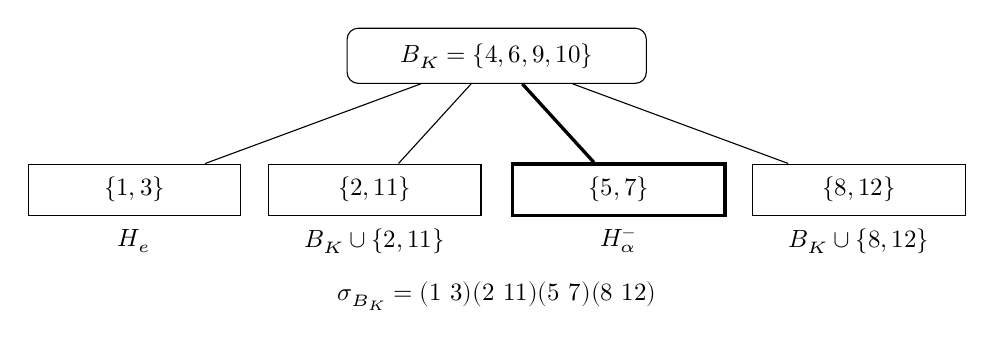
\begin{tikzpicture}[x=1cm,y=1cm, every node/.style={font=\small}]
 \node[draw,rounded corners,minimum width=3.8cm,minimum height=.7cm]
  (b) at (0,0) {$B_K=\{4,6,9,10\}$};
 \node[draw,minimum width=2.7cm,minimum height=.65cm]
  (p1) at (-4.6,-1.7) {$\{1,3\}$};
 \node[draw,minimum width=2.7cm,minimum height=.65cm]
  (p2) at (-1.55,-1.7) {$\{2,11\}$};
 \node[draw,very thick,minimum width=2.7cm,minimum height=.65cm]
  (p3) at (1.55,-1.7) {$\{5,7\}$};
 \node[draw,minimum width=2.7cm,minimum height=.65cm]
  (p4) at (4.6,-1.7) {$\{8,12\}$};
 \draw (b) -- (p1); \draw (b) -- (p2);
 \draw[very thick] (b) -- (p3); \draw (b) -- (p4);
 \node at (-4.6,-2.35) {$H_e$};
 \node at (-1.55,-2.35) {$B_K\cup\{2,11\}$};
 \node at (1.55,-2.35) {$H^-_\alpha$};
 \node at (4.6,-2.35) {$B_K\cup\{8,12\}$};
 \node at (0,-3.05)
  {$\sigma_{B_K}=(1\ 3)(2\ 11)(5\ 7)(8\ 12)$};
\end{tikzpicture}
\caption{The concrete star of the dodecaphasic flag. Each line
indicates the union of the central four-element set with the pair at its endpoint; the
thick line marks the hexad also selected by the signs
preceding the carry of $\alpha$. The four pairs exhaust the eight
outer positions.}
\label{exc:fig-estrella}
\end{figure}

\begin{proposition}[The collection of stars]
\label{exc:m12}
The $\binom{12}4=495$ permutations $\sigma_B$ preserve $\mathcal H$.
The group they generate has order $95040$ and is the Mathieu group
$M_{12}$ in its action on the small Witt design.
\end{proposition}

\begin{proof}
The preservation claim is a finite check on the
$132$ hexads of \eqref{exc:codigo}: for each four-element set the
four petals are constructed and one verifies
$\{\sigma_B(H):H\in\mathcal H\}=\mathcal H$.
Closure under composition of these permutations produces $95040$
elements. In the lexicographic enumeration, it suffices to add successively
six stars not yet contained in the group; the intermediate orders
are $2,6,18,360,7920,95040$, and all $495$ stars belong to the final
group. In image notation for \(1,\ldots,12\), the generators are
\[
\begin{aligned}
 \sigma_1&=(1,2,3,4,12,11,9,10,7,8,6,5),\\
 \sigma_2&=(1,2,3,12,5,10,11,9,8,6,7,4),\\
 \sigma_3&=(1,2,3,11,10,6,8,7,12,5,4,9),\\
 \sigma_4&=(1,2,12,4,5,9,8,7,6,11,10,3),\\
 \sigma_5&=(1,12,3,4,5,8,10,6,11,7,9,2),\\
 \sigma_6&=(12,2,3,4,5,7,6,11,10,9,8,1).
\end{aligned}
\]
For \(1\leq r\leq6\), set \(G_{r,0}=\{\operatorname{id}\}\) and iterate
\[
 G_{r,n+1}=G_{r,n}\cup\bigcup_{j=1}^{r}\sigma_jG_{r,n}.
\]
The iteration stops when \(G_{r,n+1}=G_{r,n}\); the six stabilized
cardinalities are those stated above. This specifies both the enumeration
and its finite inputs. Finally, one applies the recognition
of the automorphism group of $S(5,6,12)$ as $M_{12}$, whose order is
$12\cdot11\cdot10\cdot9\cdot8=95040$.
\end{proof}

An individual star generates a cyclic group of order two. It does
not by itself generate $M_{12}$, still less the Monster. Nor does the
existence of $495$ generators of a permutation group prove that
each is the transport of a specific TPK loop. That assertion
requires the corresponding loop map; the result established here
is the finite incidence action.

\begin{remark}[Equality of traces does not identify operators]
On $V_{11}$, a star has spectrum $+1$ with multiplicity seven
and $-1$ with multiplicity four. Its normalized trace is $3/11$.
A rank-three projector on the same space also has normalized
trace $3/11$, but spectrum $1^3,0^8$. They are not conjugate: their
minimal polynomials and spectra differ. The intertwiner
\eqref{exc:incidencia} transports defined operators; it does not turn
this scalar coincidence into an equivalence of operators.
\end{remark}

% Additive recovery from the Witt v4--v7 owners and their original tables.
% Full provenance is retained in the editorial map.
\subsection{Three regional stars and the polarization of their completions}
\label{star27:comparacion}

The preceding incidence construction compares the regions through one
operation. The regional words arise from APP--TRIT--TPK emission;
their encoding by \(\gamma_{A_W}(w)=(w,wA_W)\) retains a support
on the twelve positions. The register \(K\) and the pre-carry
cochain add two readings of the same state: position relative to
the \(729+271\) boundary and the orientation of borrowing.
The following comparison assembles these previously constructed
data while retaining their causal order.

The conserved tables also use an equivalent presentation. With
\(D=\operatorname{diag}(1,-1,-1,-1,-1,-1)\) over
\(\mathbb F_3\), their matrix is \(A_{\rm hist}=A_WD\), and
\[
\gamma_{A_{\rm hist}}(w)=\gamma_{A_W}(w)(I_6\oplus D).
\]
This change multiplies coordinates by units and preserves every
support. The star tables therefore transfer in full to the
presentation \(A_W\) used here.

Write
\[
\begin{aligned}
w_\pi&=010211,&w_e&=201101,&
w_\varphi&=121200,&w_{\rm APP}&=022020,\\
P_\pi&=\{2,4,5,6,7,8,9,10,11\},&
H_e&=\{1,3,4,6,9,10\},\\
H_\varphi&=\{1,2,3,4,7,9\},&
H_{\rm APP}&=\{2,3,5,10,11,12\}.
\end{aligned}
\]
The four sets in the second and third lines are the supports of
the corresponding encoded words. The cochain
\[
s=(7,297,353,-430,-715,-1199,-3,286,-894,-528,380,663)
\]
determines the partition
\[
H^-_\alpha=\{4,5,6,7,9,10\},\qquad
H^+_\alpha=\{1,2,3,8,11,12\}.
\]
The signs are thus fixed before decimal normalization. For a
four-subset \(B\), denote the matching of its star by
\[
\mu_W(B)=\{H\setminus B:H\in\mathcal H,\ B\subset H\}.
\]
A pair has type \(++\), \(--\), or \(+-\) according as it
contains zero, two, or one point of \(H^-_\alpha\).
Its signature is
\(\nu(B)=(n_{++}(B),n_{--}(B),n_{+-}(B))\).

\begin{proposition}[Comparison of the three regional intersections]
\label{star27:tres}
The four-subsets
\[
B_K=H_e\cap P_\pi,\qquad
B_\varphi=H_\varphi\cap P_\pi,\qquad
B_{\rm APP}=H_{\rm APP}\cap P_\pi
\]
have the twelve completions and signatures listed in
Table~\ref{star27:tabla-tres}.
\end{proposition}

\begin{table}[htbp]
\centering\small
\begin{tabular}{lll}
\toprule
Four-subset and signature & Added pair & Resulting hexad\\
\midrule
\(B_K=\{4,6,9,10\}\) & \(\{1,3\}_{++}\) & \(\{1,3,4,6,9,10\}\)\\
\(\nu(B_K)=(3,1,0)\) & \(\{2,11\}_{++}\) & \(\{2,4,6,9,10,11\}\)\\
 & \(\{5,7\}_{--}\) & \(\{4,5,6,7,9,10\}\)\\
 & \(\{8,12\}_{++}\) & \(\{4,6,8,9,10,12\}\)\\
\midrule
\(B_\varphi=\{2,4,7,9\}\) & \(\{1,3\}_{++}\) & \(\{1,2,3,4,7,9\}\)\\
\(\nu(B_\varphi)=(1,0,3)\) & \(\{5,11\}_{+-}\) & \(\{2,4,5,7,9,11\}\)\\
 & \(\{6,12\}_{+-}\) & \(\{2,4,6,7,9,12\}\)\\
 & \(\{8,10\}_{+-}\) & \(\{2,4,7,8,9,10\}\)\\
\midrule
\(B_{\rm APP}=\{2,5,10,11\}\) & \(\{1,4\}_{+-}\) & \(\{1,2,4,5,10,11\}\)\\
\(\nu(B_{\rm APP})=(1,1,2)\) & \(\{3,12\}_{++}\) & \(\{2,3,5,10,11,12\}\)\\
 & \(\{6,7\}_{--}\) & \(\{2,5,6,7,10,11\}\)\\
 & \(\{8,9\}_{+-}\) & \(\{2,5,8,9,10,11\}\)\\
\bottomrule
\end{tabular}
\caption{The three stars with the same reference polarization.
Each row retains the four-subset, complementary pair, and complete hexad.}
\label{star27:tabla-tres}
\end{table}

\begin{proof}
Applying \(\gamma_{A_W}\) to the four regional words yields
the stated supports. For each four-subset, enumerate the hexads
of \(\mathcal H\) that contain it. The relation \(\lambda_4=4\)
ensures that the four completions in the table exhaust the star.
Finally, intersection of each pair with \(H^-_\alpha\)
determines its sign. Every operation takes place within the
finite design already constructed.
\end{proof}

The three signatures distinguish concrete incidence roles.
The star of \(B_K\) separates three positive pairs and one
negative pair; that of \(B_\varphi\) contains three mixed pairs;
that of \(B_{\rm APP}\) combines all three classes. The
distinction persists even when two stars share the pair
\(\{1,3\}\).

\begin{figure}[htbp]
\centering
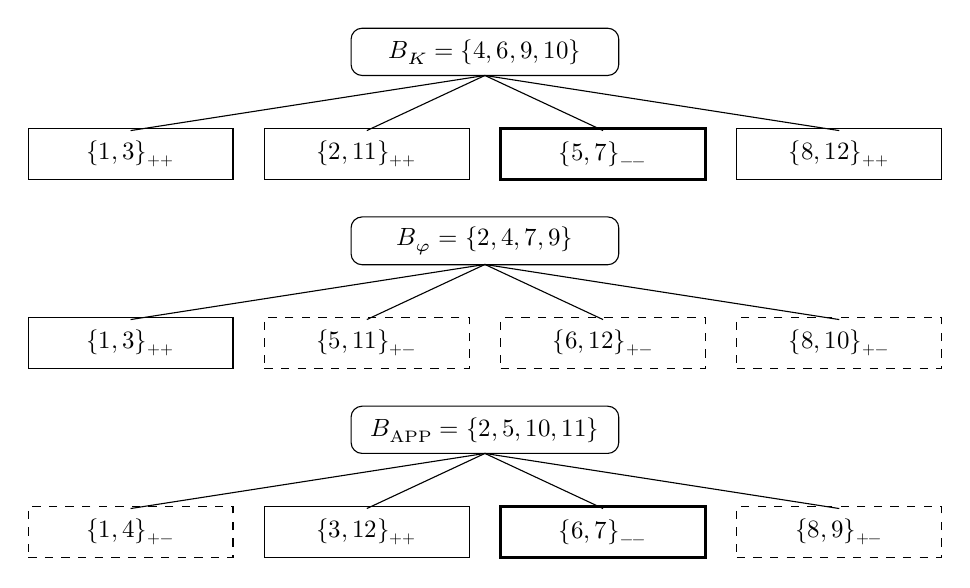
\begin{tikzpicture}[x=1cm,y=1cm,every node/.style={font=\small},
 core/.style={draw,rounded corners,minimum width=3.4cm,minimum height=.6cm},
 petal/.style={draw,minimum width=2.6cm,minimum height=.65cm}]
\foreach \y/\name in {0/{B_K=\{4,6,9,10\}},
 -2.4/{B_\varphi=\{2,4,7,9\}},-4.8/{B_{\rm APP}=\{2,5,10,11\}}}
 {\node[core] at (0,\y) {\(\name\)};
  \foreach \x in {-4.5,-1.5,1.5,4.5}
    {\draw (0,\y-.3)--(\x,\y-1);}}
\node[petal] at (-4.5,-1.3) {\(\{1,3\}_{++}\)};
\node[petal] at (-1.5,-1.3) {\(\{2,11\}_{++}\)};
\node[petal,very thick] at (1.5,-1.3) {\(\{5,7\}_{--}\)};
\node[petal] at (4.5,-1.3) {\(\{8,12\}_{++}\)};
\node[petal] at (-4.5,-3.7) {\(\{1,3\}_{++}\)};
\node[petal,dashed] at (-1.5,-3.7) {\(\{5,11\}_{+-}\)};
\node[petal,dashed] at (1.5,-3.7) {\(\{6,12\}_{+-}\)};
\node[petal,dashed] at (4.5,-3.7) {\(\{8,10\}_{+-}\)};
\node[petal,dashed] at (-4.5,-6.1) {\(\{1,4\}_{+-}\)};
\node[petal] at (-1.5,-6.1) {\(\{3,12\}_{++}\)};
\node[petal,very thick] at (1.5,-6.1) {\(\{6,7\}_{--}\)};
\node[petal,dashed] at (4.5,-6.1) {\(\{8,9\}_{+-}\)};
\end{tikzpicture}
\caption{Comparison of the three stars. Each connection represents
the union of the upper four-subset with one pair; the twelve complete
hexads appear in Table~\ref{star27:tabla-tres}. Thick outlines
indicate negative pairs and dashed outlines mixed pairs.
The connections represent incidence.}
\label{star27:figura}
\end{figure}

\begin{proposition}[Coupling of corona, incidence, and sign]
\label{star27:acoplamiento}
For the previously constructed dodecaphasic register,
\[
B_K=\{i:K_i\geq729\}=H_e\cap P_\pi=\{4,6,9,10\}.
\]
The unique hexad \(H\in\mathcal H\) satisfying
\(H\cap P_\pi=B_K\) is \(H_e\). Moreover,
\[
H^-_\alpha=B_K\sqcup\{5,7\},\qquad
(B_\varphi\setminus B_K)\cap H^-_\alpha=\{7\}.
\]
\end{proposition}

\begin{proof}
The register
\(K=(234,543,140,729,659,824,621,58,914,794,146,601)\)
reaches or exceeds \(729\) at precisely the four stated
positions. Comparison with the supports proves the first
equality. A hexad with intersection \(B_K\) belongs to
the star of \(B_K\); among its four pairs, only
\(\{1,3\}\) is disjoint from \(P_\pi\). This proves
the relative uniqueness of \(H_e\). The table identifies
the negative pair \(\{5,7\}\). Finally,
\(B_\varphi\setminus B_K=\{2,7\}\), and the signs
\(s_2=297>0\), \(s_7=-3<0\) determine the pivot \(7\).
\end{proof}

The four-subset, sign, and normalization retain distinct roles.
Incidence fixes the completion \(H^-_\alpha\); the Archimedean
lift of the complete cochain also uses the magnitudes, positional
order, and carries already established in the closure of
\(\alpha\). This composition explains how one genealogy
produces both a geometric boundary reading and a numerical reading.

\subsection{Polarized classification of the 495 four-subsets}
\label{star27:clasificacion}

\begin{theorem}[Signature census and regional restriction]
\label{star27:censo}
The \(495=\binom{12}{4}\) four-subsets are distributed as
in Table~\ref{star27:tabla-censo}. The last column counts
hexads \(H\) with \(|H\cap P_\pi|=4\), classified by
\(\nu(H\cap P_\pi)\).
\end{theorem}

\begin{table}[htbp]
\centering
\begin{tabular}{ccc}
\toprule
\(\nu=(n_{++},n_{--},n_{+-})\)&Four-subsets&Regional hexads\\
\midrule
\((3,1,0)\)&15&9\\
\((1,3,0)\)&15&0\\
\((2,2,0)\)&45&9\\
\((1,1,2)\)&180&18\\
\((1,0,3)\)&120&18\\
\((0,1,3)\)&120&0\\
\midrule
Total&495&54\\
\bottomrule
\end{tabular}
\caption{Complete classification and restriction to the support
\(P_\pi\). The two columns count different objects: four-subsets
and hexads.}
\label{star27:tabla-censo}
\end{table}

\begin{proof}
The following procedure is an exact enumeration of the finite
domain. Form the \(3^6\) words \(w\), compute \((w,wA_W)\)
modulo \(3\), and retain their weight-six supports without
repetition. This gives \(\mathcal H\), with \(132\) elements.
For each \(B\in\binom{[12]}4\), form \(\mu_W(B)\), count
the intersections of its four pairs with \(H^-_\alpha\),
and increment the entry for the resulting signature. The six
counts are \(15,15,45,180,120,120\). They sum to \(495\),
and each four-subset is processed once. For the last column,
traverse the \(132\) hexads, retain the \(54\) whose
intersection has size four, and apply the same function
\(\nu\) to that intersection. The operations are set
comparisons and arithmetic in \(\mathbb F_3\); the
reproducible certificate retains the complete input--output table.
\end{proof}

The signature \((3,1,0)\) occurs for fifteen four-subsets.
The regional frame is characterized jointly by the corona of
\(K\), the intersection \(H_e\cap P_\pi\), and the cochain
sign, as established in Proposition~\ref{star27:acoplamiento}.

\subsection{Rigidity of the ordered four-support frame}
\label{star27:rigidez}

Let \(G_W=\langle\sigma_B:|B|=4\rangle\), already computed
in Proposition~\ref{exc:m12}. For an ordered collection of
supports, define
\[
\operatorname{Stab}_{G_W}(S_1,\ldots,S_r)
=\{g\in G_W:g(S_j)=S_j\ \text{for every }j\}.
\]
Each support is preserved individually; internal permutations
of its points remain permitted.

\begin{theorem}[Joint rigidity of the four incidences]
\label{star27:marco}
The stabilizers have the following orders:
\[
\begin{array}{l|r}
\text{preserved data}&\text{order}\\ \hline
H^-_\alpha&720\\
H^-_\alpha,\ 6&120\\
B_K&192\\
B_K,H^-_\alpha&48\\
B_K,H^-_\alpha,H_e&16\\
H^-_\alpha,H_e,H_\varphi&2\\
H^-_\alpha,H_e,H_\varphi,H_{\rm APP}&1
\end{array}
\]
The second row also preserves the point \(6\).
In particular,
\[
\operatorname{Stab}_{G_W}
(H^-_\alpha,H_e,H_\varphi,H_{\rm APP})=\{\operatorname{id}\}.
\]
\end{theorem}

\begin{proof}
Use the closure under composition of the six explicit
permutations in Proposition~\ref{exc:m12}. On its \(95040\)
elements evaluate the predicates \(g(S_j)=S_j\), together
with \(g(6)=6\) where required. Summing their indicators
gives \(720,120,192,48,16,2,1\), respectively. The identity
satisfies every condition; the last cardinality proves
that it is the unique element. The closure algorithm
terminates when the set stabilizes, and the stabilizer
filters are then applied to the complete group.
\end{proof}

The table compares seven marked configurations. Two useful
inclusion chains are those determined by
\((B_K)\), \((B_K,H^-_\alpha)\),
\((B_K,H^-_\alpha,H_e)\), and by
\((H^-_\alpha)\), \((H^-_\alpha,H_e,H_\varphi)\),
\((H^-_\alpha,H_e,H_\varphi,H_{\rm APP})\).
Final rigidity means that the ordered regional frame fixes
all residual freedom within \(G_W\). Its domain is the
action on twelve positions; subsequent transport to
lattices and algebras retains the maps belonging to
those realizations.

\subsection{Finite incidence topology and preservation of its domain}
\label{star27:topologia}

The simplicial complex generated by the \(132\) hexads
has face vector
\[
(f_0,f_1,f_2,f_3,f_4,f_5)=(12,66,220,495,792,132)
\]
and Euler characteristic
\(\chi=12-66+220-495+792-132=331\).
Indeed, each five-subset has a unique hexadic extension;
every smaller subset belongs to one of these five-subsets,
and the maximal faces are the hexads.

The bipartite graph between four-subsets and hexads has
\[
|V|=495+132=627,\qquad |E|=495\cdot4=132\cdot15=1980.
\]
It is connected. Let \(H,H_*\) be distinct hexads; their
intersection has at most four points because each five-subset
has a unique extension. Choose a four-subset \(B\subset H\)
containing \(H\cap H_*\), and a point \(p\in H_*\setminus H\).
The unique extension \(H'\) of \(B\cup\{p\}\) is joined to
\(H\) by the bipartite path \(H-B-H'\) and satisfies
\(|H'\cap H_*|>|H\cap H_*|\). Repeating the operation
reaches \(H_*\); containing five of its points already
forces equality. Every four-subset is incident to four
hexads, so it too belongs to this single component.
Its first Betti number is therefore
\[
\beta_1=|E|-|V|+1=1354.
\]
An exhaustive traversal also verifies connectedness.
For unordered pairs of distinct hexads, the intersection
census is
\[
\begin{array}{c|rrrr}
|H\cap H'|&0&2&3&4\\ \hline
\#\{H,H'\}&66&2970&2640&2970 .
\end{array}
\]
The sum \(8646=\binom{132}{2}\) covers every pair.

These invariants describe the complex and its incidence graph.
The junction micrograph \(U_6=A|B\) separately retains its
\(96\) vertices, \(234\) edges, six components, and
\(\beta_1=234-96+6=144\). Likewise, compositions of the
\(\sigma_B\) act on incidence positions, whereas
\(\Gamma_9\) transports the TPK state with memory.
This distinction relates the readings through their
effective maps and preserves, at each level, the data
used by the operation.


\subsection{The binary residue and the five regions of \texorpdfstring{$\pi$}{pi}}
\label{exc:cinco-regiones}

The next recognition uses the extended binary Golay code
$G_{24}$, with parameters $[24,12,8]_2$. Its weights are
$0,8,12,16,24$, and the weight-eight supports form the design
$S(5,8,24)$. Fix a dodecad $D$, the support of a weight-twelve
word. This datum and the incidence isomorphism to be declared
below belong to the realization chart; they are not used to
generate or select the decimals of $\pi$.

\begin{proposition}[Residue of a dodecad and lifting of hexads]
\label{exc:residuo-binario}
The set
\[
 \mathcal H(D)=
 \{O\cap D: O\text{ is an octad},\ |O\cap D|=6\}
\]
is an $S(5,6,12)$ system on $D$. Each of its hexads has
a unique lift to an octad. For any four-element set $B\subset D$,
the five octads containing it split into four residual
lifts and a unique octad $O_B^\perp$ with $O_B^\perp\cap D=B$.
\end{proposition}

\begin{proof}
A five-element set $A\subset D$ belongs to a unique octad $O$. If
$j=|O\cap D|$, the binary word given by the sum of $O$ and $D$ has weight
$20-2j$. Among the permitted weights, with $0\leq j\leq8$, only
$j=2,4,6$ are possible. Since $A\subset O\cap D$, we have $j\geq5$
and therefore $j=6$. This gives existence and uniqueness of the residual
hexad, as well as uniqueness of its lift by selecting five of its
points. Moreover,
\[
 \lambda_4(S(5,8,24))=\frac{\binom{20}1}{\binom41}=5,
 \qquad
 \lambda_4(S(5,6,12))=4.
\]
The four residual hexads on $B$ give four distinct octads.
The fifth cannot meet $D$ in six points, since it would be another residual
hexad; because it contains $B$, its intersection has size four and
equals $B$.
\end{proof}

A hexad-preserving chart $\ell:[12]\to D$ identifies
$\mathcal H$ with $\mathcal H(D)$. Its existence is the recognition
of the design already constructed as the small Witt design; a concrete
choice of $\ell$ fixes the relabeling. The lift
\[
 \iota_D:\mathcal H\longrightarrow
       \{\text{octads of }G_{24}\},
 \qquad H\longmapsto O\text{ such that }O\cap D=\ell(H),
\]
is injective because intersection with $D$ recovers $\ell(H)$.
The domain of this injectivity is the hexads, not the record $K$.

The relation to the five regions of $\pi$ preserves richer data
than the number five. The emissions and their signatures are:
\begin{center}
\small
\begin{tabular}{@{}crll@{}}
\toprule
Region & Multiplicity & Emission $U_6$ & Signature \\
\midrule
$\perp$ & $432$ & $(501,614,498,169,272,272)$ & $555555$ \\
$++_1$ & $144$ & $(810,923,870,169,272,272)$ & $339555$ \\
$++_2$ & $144$ & $(810,983,810,169,272,272)$ & $393555$ \\
$++_3$ & $144$ & $(870,923,810,169,272,272)$ & $933555$ \\
$--$ & $144$ & $(870,923,810,418,674,521)$ & $933717$ \\
\bottomrule
\end{tabular}
\end{center}
In each three-digit decimal block, the signature uses the modular
difference of the first two digits. The five emissions have the
same visible tritic word $w_\pi=010211$, but not the same
regional genealogy. The three positive regions preserve the tail
$169|272|272$; the negative region changes it to $418|674|521$;
the transverse region has a constant signature and greater multiplicity.

The marked extension of the regional chart sends the transverse region
to $O_{\ell(B_K)}^\perp$, the negative region to $\iota_D(H^-_\alpha)$, and the
three positive regions to the other three lifts of the star. This
realizes the $4+1$ partition of the five octads on $\ell(B_K)$.
The individual correspondence between the three positive names and
the three remaining petals requires a chart order; incidence does not
determine it without that datum. The precise claim is therefore a
marked correspondence of regions, compatible with their roles and with
the flag, not a canonical bijection inferred from the cardinality five.

The identity $432+4\cdot144=1008$ preserves the regional
multiplicities. Also, $1008=36\cdot28$, and an octad has
$\binom82=28$ pairs. These equalities are arithmetic catalog
checks, not substitutes for the map $\iota_D$ or the regional chart.

\subsubsection{Pentadic representation of the microfiber and its incidence}
\label{pi-estrella:desarrollo}

The arrangement of the five regions makes it possible to visualize simultaneously
the unity of the ternary quotient and the differentiation preserved by the
catalog. The relevant map is the restriction
\[
 \Psi\big|_{\mathscr R_\pi^{\rm micro}}:
 \mathscr R_\pi^{\rm micro}\longrightarrow\{010211\},
 \qquad \Psi(U)=(-U)\bmod3.
\]
Its five antecedents are the vectors \(U_6\) in the preceding table.
Figure \ref{pi-estrella:figura} recovers their radial organization,
preserving chart order, signatures, and multiplicities of the
catalog.

% Chart order and data recovered from fig_cinco_regiones_pi.tex.
\begin{figure}[H]
\centering
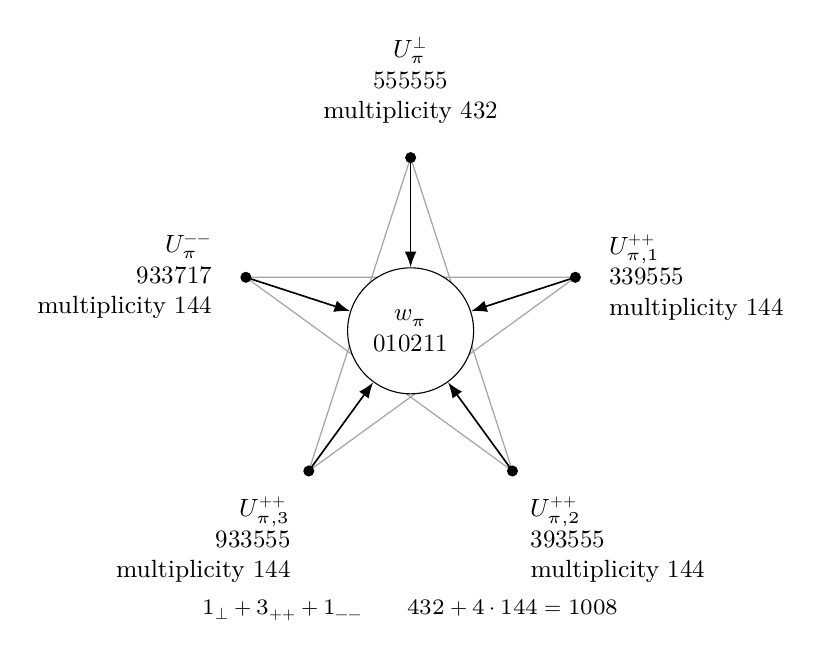
\begin{tikzpicture}[x=1cm,y=1cm,font=\small,>=Latex]
 \coordinate (a) at (90:2.2);
 \coordinate (b) at (18:2.2);
 \coordinate (c) at (-54:2.2);
 \coordinate (d) at (-126:2.2);
 \coordinate (e) at (162:2.2);
 \draw[black!35,line width=.45pt]
    (a)--(c)--(e)--(b)--(d)--cycle;
 \node[draw,fill=white,circle,minimum size=1.6cm,align=center,
    inner sep=3pt] (z) at (0,0) {$w_\pi$\\$010211$};
 \foreach \v in {a,b,c,d,e}{
    \fill (\v) circle (2pt);
    \draw[->,line width=.6pt] (\v)--(z);
 }
 \node[above=3mm,align=center] at (a)
   {$U_\pi^\perp$\\$555555$\\multiplicity $432$};
 \node[right=3mm,align=left] at (b)
   {$U_{\pi,1}^{++}$\\$339555$\\multiplicity $144$};
 \node[below right=2mm and 1mm,align=left] at (c)
   {$U_{\pi,2}^{++}$\\$393555$\\multiplicity $144$};
 \node[below left=2mm and 1mm,align=right] at (d)
   {$U_{\pi,3}^{++}$\\$933555$\\multiplicity $144$};
 \node[left=3mm,align=right] at (e)
   {$U_\pi^{--}$\\$933717$\\multiplicity $144$};
 \node[align=center,font=\footnotesize] at (0,-3.55)
   {$1_\perp+3_{++}+1_{--}$\qquad $432+4\cdot144=1008$};
\end{tikzpicture}
\caption{The five regions of \(\pi\) in a pentadic arrangement.
Each position preserves its multiplicative signature and multiplicity;
the radial arrows represent the common projection
\(\Psi(U)=010211\). The star-shaped outline organizes the five
positions of the chart. Their realization in the five Witt octads
is performed through regional alignment and the
\(4+1\) decomposition in the text.}
\label{pi-estrella:figura}
\end{figure}


Projection onto the center identifies the five ternary images; the
record of exterior positions retains the regional information
making incidence realization possible. The distribution
\(1_\perp+3_{++}+1_{--}\) specifies one transversal region, three
positive regions, and one negative region. Their normalized weights are
\(3/7\) and \(1/7\) for each of the remaining four: transversal
multiplicity is triple, even though all five images under
\(\Psi\) coincide.

\Needspace{11\baselineskip}
The link with the Witt star is formulated through the flag
\(B_K\subset H^-_\alpha\), the alignment \(\ell\), and the
lift \(\iota_D\) already constructed. The five regional positions
are realized in the five octads over \(\ell(B_K)\):
\[
\begin{aligned}
 U_\pi^\perp&\longmapsto O^\perp_{\ell(B_K)},\\
 U_\pi^{--}&\longmapsto\iota_D(H^-_\alpha),\\
 \{U_{\pi,1}^{++},U_{\pi,2}^{++},U_{\pi,3}^{++}\}
 &\longmapsto
 \{\iota_D(B_K\cup P):P\in\mathcal P_+\},\\
 \mathcal P_+&=\bigl\{\{1,3\},\{2,11\},\{8,12\}\bigr\}.
\end{aligned}
\]
Assignment of the three positive positions to the three pairs is
performed in an ordered chart. The transversal and negative rows
are distinguished by their regional predicates and by the flag.

The two figures are thus articulated: Figure
\ref{exc:fig-estrella} shows the four hexads of the small Witt
design over \(B_K\); Figure \ref{pi-estrella:figura} shows
the five regions that, under alignment, occupy the four residual
octads and the transversal octad of the binary design. The law
\(4+1\), proved in Proposition
\ref{exc:residuo-binario}, specifies the change in incidence. In this
composition, \(K\) determines the marked tetrad, and the signature of
\(\alpha\) distinguishes one of its hexads. In addition to their common
ternary value, the regions preserve the structure required for that
transport toward the exceptional realization.


\subsection{From the ternary code to the Niemeier lattice}
\label{exc:niemeier}

The passage to dimension twenty-four need not first go through the
binary code. It is performed directly from $C_W$ by discriminant
gluing. Two compatible prolongations thus remain distinct:
one preserves the residue $W_{12}\subset W_{24}$; the other constructs the
lattice on which the vertex operator algebra will be realized.

Let $A_2=\mathbb Z a_1\oplus\mathbb Z a_2$ with Gram matrix
\[
 \begin{pmatrix}2&-1\\-1&2\end{pmatrix},
 \qquad \rho=a_1+a_2,\qquad \rho^2=2.
\]
Represent the three classes of $A_2^*/A_2$ by
\[
 \varpi_0=0,\qquad
 \varpi_1=\frac{2a_1+a_2}{3},\qquad
 \varpi_2=\frac{a_1+2a_2}{3}.
\]
The map $j\mapsto\varpi_j+A_2$ additively identifies
$\mathbb F_3$ with this discriminant. For $c\in C_W$, write
$\phi(c)=(\varpi_{c_1},\ldots,\varpi_{c_{12}})$ and define
\begin{equation}
 N(C_W)=\bigcup_{c\in C_W}\bigl(A_2^{12}+\phi(c)\bigr).
 \label{exc:niemeier-def}
\end{equation}

\begin{theorem}[Ternary gluing]
\label{exc:niemeier-teorema}
The object \eqref{exc:niemeier-def} is a positive, even,
unimodular lattice of rank $24$. Its root system is exactly
$A_2^{12}$; it is therefore recognized as the Niemeier lattice with
that root system.
\end{theorem}

\begin{proof}
Linearity of the code makes the union of classes stable under
addition. Self-orthogonality annihilates the discriminant pairing:
the latter is a multiple of $c\cdot d/3$ modulo $\mathbb Z$. Thus the
lattice is integral. The norm of a glue class is
$2\operatorname{wt}(c)/3$ modulo $2\mathbb Z$. The weights in
\eqref{exc:enumerador} are multiples of three, so the lattice is even.

The index of $A_2^{12}$ in $N(C_W)$ is $|C_W|=3^6$. Consequently,
\[
 \det N(C_W)=\frac{3^{12}}{(3^6)^2}=1.
\]
Positivity follows from the orthogonal sum of the twelve $A_2$ metrics.
In a nonzero class of $A_2^*/A_2$, the minimum norm is $2/3$;
every nonzero word has at least six nonzero positions.
Hence a vector in a nontrivial glue class has norm
at least $6\cdot2/3=4$. No norm-two roots occur outside
$A_2^{12}$. Within it, the roots are precisely those of its
twelve components.
\end{proof}

\subsection{Incidence selection of the rootless unimodular neighbor}
\label{exc:leech}

\paragraph{From the incidence origin to lattice modification.}
\label{inc-ampl-reticulo}
The marked flag determines a position through an equivariant
set operation:
\[
 o_*=(H_e\cap H_\varphi)
       \setminus(H^-_\alpha\cup H_{\rm APP})=\{1\}.
\]
Its function is to distinguish one component among the twelve entering
the lattice realization. The complete ternary code
acts as a glue code in the discriminant module
$(A_2^*/A_2)^{12}$. Its preimage defines $N(C_W)$, and
self-duality, weights, and distance of the code translate,
respectively, into properties of integrality and determinant, parity,
and norm bounds for the glue classes. Here the symbolic information
of the code performs a function no longer performed by the isolated support.

The $A_2$ metric and positive radial chamber are fixed in the lattice
development. Within that chamber, the congruence required for an even
index-three neighbor has twelve realizations of minimum norm $54$,
permuted by changing the distinguished component. The origin $o_*$
selects
\[
 v_\alpha=4\rho_1+\rho_2+\cdots+\rho_{12},\qquad
 v_\alpha^2=2(4^2+11)=54.
\]
The coefficient $4$ belongs to that solution of the congruence in the
declared chamber. The subscript $\alpha$ records the incidence
provenance of the selection: its content is the frame that entered
closure and now individualizes a lattice direction.

Pairing with $v_\alpha$ determines the index-three sublattice
$N_{\alpha,0}$, and adding the class
$v_\alpha/3$ produces the neighbor $N_\alpha$ of
\eqref{exc:vecino}. This modification preserves rank and recovers
unimodularity and parity; congruence selection eliminates the previous
roots, and local bounds exclude roots in the new classes.
Identification with Leech appears after these verifications. The
binary realization of the five regions and this lattice construction
are two prolongations of the common frame: the second receives the
ternary code directly as glue data.


The label $o_*=1$ of the flag is now realized as one of the
twelve $A_2$ components. This operation declares the preceding metric and
the positive radial chamber
\[
 v(a)=\sum_{i=1}^{12}a_i\rho_i,
 \qquad a_i=1+3b_i,\quad b_i\in\mathbb Z_{\geq0}.
\]
The evenness requirement for the index-three neighbor is
$v(a)^2\equiv0\pmod{18}$. Since
\[
 v(a)^2=2\sum_i(1+3b_i)^2,
\]
this congruence is equivalent to $\sum_i b_i\equiv1\pmod3$. The least
norm in the chamber is obtained with a single $b_i=1$ and
all others zero; it is $54$. The marked origin selects
\begin{equation}
 v_\alpha=4\rho_1+\rho_2+\cdots+\rho_{12},
 \qquad v_\alpha^2=54.
 \label{exc:vector}
\end{equation}
The word ``least'' refers to this positive chamber. It does not assert
minimality throughout the residual class: the vector
$(a_1-2a_2,\rho,\ldots,\rho)$ represents the same class modulo three
and has norm $14+11\cdot2=36$. The chamber restriction is part
of the construction data, not an omissible conclusion.

Let $N=N(C_W)$. Define
\begin{equation}
 N_{\alpha,0}=\{x\in N:\langle x,v_\alpha\rangle\equiv0\pmod3\},
 \qquad
 N_\alpha=N_{\alpha,0}+\mathbb Z\frac{v_\alpha}{3}.
 \label{exc:vecino}
\end{equation}

\begin{theorem}[Leech neighbor determined by the marked flag]
\label{exc:teorema-leech}
With the declared metric and chamber, $N_\alpha$ is a positive, even,
unimodular lattice of rank $24$, with no vectors of norm two.
By the corresponding classification theorem, it is isometric to the
Leech lattice $\Lambda_{24}$.
\end{theorem}

\begin{proof}
The character $x\mapsto\langle x,v_\alpha\rangle\bmod3$ is nonzero:
a simple root of a component pairs with $a_i\rho_i$ to give
$a_i\equiv1\pmod3$. Hence $[N:N_{\alpha,0}]=3$ and
$\det N_{\alpha,0}=9$. Moreover,
$v_\alpha/3\in N_{\alpha,0}^*$ and $v_\alpha\in N_{\alpha,0}$.
If $v_\alpha/3$ belonged to $N$, the integrality of $N$ would make
all pairings with $v_\alpha$ divisible by three,
contradicting the nonzero character. The class of $v_\alpha/3$ therefore
has order three. It follows that
\[
 [N_\alpha:N_{\alpha,0}]=3,
 \qquad \det N_\alpha=9/3^2=1.
\]
The extension is integral, and for $x\in N_{\alpha,0}$,
\[
 \left(x+m\frac{v_\alpha}{3}\right)^2
   =x^2+2m\frac{\langle x,v_\alpha\rangle}{3}+6m^2
   \in2\mathbb Z.
\]
Hence it is even.

It remains to exclude roots, the decisive step. The roots of $N$
belong to $A_2^{12}$. Their pairings with $v_\alpha$ are
congruent to $\pm1$ or $\pm2$ modulo three; none belongs to
$N_{\alpha,0}$. For the other two classes of the neighbor, each component
belongs to one of the local classes
\[
 A_2+\varpi_j\pm\rho/3,\qquad j=0,1,2.
\]
Since $4\rho/3\equiv\rho/3\pmod{A_2}$, this description also holds
in the distinguished component. Writing a local vector
as $(u a_1+v a_2)/3$, its norm is
$2(u^2-uv+v^2)/9$. The six preceding classes have nonzero residues
and minimum $2/9$: representatives minimizing the quadratic form
are $(\pm1,0),(0,\pm1),(1,1),(-1,-1)$ in the appropriate residues.
A vector in a new class therefore has norm at least
$12\cdot2/9=8/3>2$. There are no roots in any of the three classes.
The classification of positive even unimodular lattices of
rank twenty-four identifies the unique rootless case with
$\Lambda_{24}$.
\end{proof}

The argument does not recognize Leech from a coincidence of dimension.
It constructs the gluing, proves integrality, evenness, and the determinant, and
eliminates roots through a local bound. Only then does it apply the
classification theorem. The dependence on $\alpha$ is preserved in
the flag selecting $o_*$ and in the vector \eqref{exc:vector};
the scalar value of the constant is not converted into a length of the
lattice.

\subsection{The vertex operator algebra and the Monster}
\label{exc:voa}

Let $\Lambda=N_\alpha$, already recognized as Leech. The next step
uses its integral lattice, not a decimal expansion. The lattice
vertex operator algebra construction is written
\[
 V_\Lambda=M(1)\otimes\mathbb C_\varepsilon[\Lambda].
\]
Here $M(1)$ is the rank-twenty-four Heisenberg oscillator
space; $\mathbb C_\varepsilon[\Lambda]$ is the group algebra
twisted by the cocycle of the central extension of the lattice. The
cocycle and the lift of the isometries are part of the
construction: a bare vector-space sum does not determine the vertex
products.

Negation $\lambda\mapsto-\lambda$ admits the standard lift
$\theta$. With its twisted module and the compatible parity choice,
the Frenkel--Lepowsky--Meurman construction produces
\begin{equation}
 V^\natural_{\rm HMT}
   =V_\Lambda^+\oplus(V_\Lambda^T)^+.
 \label{exc:flm}
\end{equation}
The sign $+$ denotes the even part of the lifted action. The expression
includes the orbifold vertex product; it is not merely a sum
of graded spaces.

\begin{theorem}[Prolongation to the Moonshine module]
\label{exc:moonshine}
The algebra \eqref{exc:flm}, constructed on the neighbor
\eqref{exc:vecino}, is a realization of the Moonshine algebra
$V^\natural$. It has central charge $24$, zero weight-one component,
and automorphism group isomorphic to the Monster $\mathbb M$. Its graded
character is
\begin{equation}
 \operatorname{Tr}_{V^\natural_{\rm HMT}}q^{L_0-1}
   =J(\tau)=j(\tau)-744
   =q^{-1}+196884q+21493760q^2+\cdots,
 \qquad q=e^{2\pi i\tau}.
 \label{exc:j}
\end{equation}
\end{theorem}

\begin{proof}
Theorem \ref{exc:teorema-leech} verifies the lattice hypotheses:
positivity, evenness, unimodularity, rank twenty-four, and absence of
roots. The Frenkel--Lepowsky--Meurman construction and theorem
for the Leech lattice then apply. They identify
the orbifold with $V^\natural$ and establish its character and its
automorphism group. Composing the flag, the neighbor, and the VOA
construction functor gives the realization stated here. The group is not inferred
from the coefficient $196884$.
\end{proof}

The theorem used is a subsequent classical recognition with verified
hypotheses, not a new proof of the FLM construction in this article
\cite{flm}.
Moreover, the notation $q=e^{2\pi i\tau}$ is the conventional Fourier
variable used to recognize the character. It does not introduce $\pi$
or $e$ as inputs into the coinductive generator that has already determined them.

Part of the trace mechanism can be seen before the orbifold.
Only the zero lattice vector is fixed by negation; each
oscillator contributes an alternating sign. Hence
\[
 \operatorname{Tr}_{V_\Lambda}\theta q^{L_0-1}
   =t_2(\tau)
   :=q^{-1}\prod_{n\geq1}(1+q^n)^{-24}.
\]
This trace in the lattice algebra must not be confused with the
character of $V^\natural$ without insertion. Nor does it by
itself identify a Monster conjugacy class: the space, insertion,
and lift must be specified before functions are compared.

\paragraph{Grading, unity, and automorphisms.}
\label{inc-ampl-automorfismos}
The Frenkel--Lepowsky--Meurman construction is applied to the lattice
$N_\alpha$ once its properties have been verified. It incorporates the oscillator
space, the central extension of the lattice, the vertex product,
and the sector twisted by the lift of negation. The result is
the algebra $V^\natural_{\rm HMT}$ of \eqref{exc:flm}, whose
automorphism group is isomorphic to the Monster. Its action domain is thus
fixed by an algebraic structure with grading and product. Borcherds's
Moonshine theorem subsequently determines the graded traces
with insertion of those automorphisms \cite{flm,borcherds}.

Unity acquires a precise realization at this level: the weight-zero
component is the vacuum line and contributes the coefficient $1$ of
$q^{-1}$ in the graded character. At the cylinder level,
refinement maps preserve the constant function through
precomposition. Every conservation statement therefore has its
object and map. The development of the proofs makes visible this
continuity of construction, from arithmetic operations and
memory to incidence, metric, and vertex products.

This articulation places $K$ and the closure of $\alpha$ in the main
argument. $K$ reversibly preserves an integral coordinate of the
history; normalization of $\alpha$ composes regional records
with that coordinate; the signed configuration determines a flag; and
the marked flag selects the lattice modification on which
Moonshine is realized. The following proofs develop these
maps, distinguishing reversible equivalences, information
quotients, and realizations adding metric or algebraic
structure. A demonstrable relation between structure,
equation, and value is thus expressed, preserving the attribution of each construction and the
scope of its theorems.


% Additive incorporation for Article I; the preceding source is unchanged.
% RESULTADO_RECUPERADO: integral, chapter 22, extensive source
% colaboracion/partes_i_ii/source/base_residencias/
% capitulo_22_c20_lineas_2613_3270.tex, lines 176--576.
% Equivalence 2/3: public/residencias/capitulo_22_voa_leech_moonshine.tex,
% lines 55--127. Order two and Fricke: hmt/15d_voa_moonshine_orden_dos_rev11.tex.
% Prerequisites resident in I: code C_W, matrix A_W, N(A_2^12),
% origin o_*, vector v_alpha of norm54, N_alpha recognized as Leech,
% lattice VOA and FLM presentation in preceding sections.
% New bibliography: chenlamshimakura2016, abelamyamada2017,
% kmconwaynorton1979.

\subsection{Ternary orientation of the Leech neighbour}
\label{km:orden-tres-reticular}

The order-two presentation constructed above uses negation
of the Leech lattice. The same lattice, obtained from the incidence marked
by \(K\) and the dodecaphasic support of \(\alpha\), admits a second
presentation compatible with the ternary character of the construction.
To make this continuity explicit, the gluing is retained, its order-three
isometry is constructed, and preservation of the already selected neighbour
is verified. This step requires no alteration of \(K\), its rational reading,
or the preceding definition of \(\alpha\). The construction presents the lattice operations and the precise conditions of the classical theorems used.

We work in the basis of simple roots of each \(A_2\) factor, with
\begin{equation}
 B_2=\begin{pmatrix}2&-1\\-1&2\end{pmatrix},\qquad
 \mathsf C=\begin{pmatrix}0&-1\\1&-1\end{pmatrix},\qquad
 \mathsf R=\begin{pmatrix}0&1\\1&0\end{pmatrix},\qquad
 \rho=\begin{pmatrix}1\\1\end{pmatrix}.
 \label{km:coxeter-reflexion}
\end{equation}
Multiplication gives
\[
 \mathsf C^3=I_2,\quad
 \mathsf C^2+\mathsf C+I_2=0,\quad
 \mathsf C^{\mathsf T}B_2\mathsf C=B_2,\quad
 \mathsf R\mathsf C\mathsf R=\mathsf C^{-1},\quad
 \mathsf R^{\mathsf T}B_2\mathsf R=B_2.
\]
These identities fix both the metric and the orientation of the action.
In the discriminant \(A_2^*/A_2\cong\mathbb F_3\), we take
the class of \(\varpi=(2,1)^{\mathsf T}/3\) as generator. We have
\(\mathsf C\varpi-\varpi=(-1,0)^{\mathsf T}\), so
\(\mathsf C\) acts trivially on the discriminant; the reflection
\(\mathsf R\) reverses its sign.

The Paley--Witt matrix already constructed produces a full-support
element by the following operation:
\begin{equation}
 \begin{gathered}
 q_*=(1,1,1,1,1,1),\qquad q_*A_W=(2,1,1,1,1,1),\\
 c_*=(q_*,q_*A_W)
 =(1,1,1,1,1,1,2,1,1,1,1,1)\in C_W.
 \end{gathered}
 \label{km:palabra-total}
\end{equation}
Every coordinate of \(c_*\) is nonzero. For the twelve positions,
define the frames and the isometry
\begin{equation}
 P_b(c_*)=
 \begin{cases}\mathsf R,&(c_*)_b=1,\\I_2,&(c_*)_b=2,\end{cases}
 \qquad
 g_c=\bigoplus_{b=1}^{12}P_b(c_*)\mathsf C P_b(c_*)^{-1}.
 \label{km:isometria-ternaria}
\end{equation}
The symbol \(P_b(c_*)\) here denotes an invertible frame of an
\(A_2\) factor, not the three-dimensional isotypic projector \(P_3\).

\begin{proposition}[Order-three isometry on the marked neighbour]
\label{km:estabilidad-vecino}
The operator \(g_c\) is an order-three isometry with no nonzero
fixed vectors. It preserves the Niemeier lattice \(N=N(C_W)\) and the
neighbour \(N_\alpha\) constructed in \eqref{exc:vecino}.
\end{proposition}
\begin{proof}
Each block of \(g_c\) is \(\mathsf C\) or \(\mathsf C^{-1}\);
its minimal polynomial is \(X^2+X+1\). This proves its order and
the absence of fixed vectors. Both blocks act trivially on the
discriminant, so they preserve every gluing class and therefore
the lattice \(N\).

Write \(v=v_\alpha=4\rho_{o_*}+\sum_{b\ne o_*}\rho_b\),
with the frames and incidence origin already fixed. Its radial
coefficients are \(a_{o_*}=4\) and \(a_b=1\) for \(b\ne o_*\).
All satisfy \(a_b\equiv1\pmod3\). In one factor,
\[
 (\mathsf C-I_2)\rho=(-2,-1)^{\mathsf T},\qquad
 (\mathsf C^{-1}-I_2)\rho=(-1,-2)^{\mathsf T}.
\]
After division by three, their discriminant classes are
\(2\) and \(1\), respectively. Consequently, the vectors
\begin{equation}
 y=\frac{g_cv-v}{3},\qquad z=\frac{g_c^{-1}v-v}{3}
 \label{km:desplazamientos}
\end{equation}
have discriminant words \(c_*\) and \(-c_*\), both in
\(C_W\). Hence \(y,z\in N\). The local product is
\[
 \left\langle
 \frac{(\mathsf C^{\pm1}-I_2)a_b\rho}{3},a_b\rho
 \right\rangle=-a_b^2,
\]
and summing gives
\(\langle y,v\rangle=\langle z,v\rangle=-(16+11)=-27\).
Thus, \(y,z\in N_0=\{x\in N:\langle x,v\rangle\equiv0\pmod3\}\).
For \(x\in N_0\),
\[
 \langle g_cx,v\rangle
 =\langle x,g_c^{-1}v\rangle
 =\langle x,v\rangle+3\langle x,z\rangle\equiv0\pmod3.
\]
The argument applied to \(g_c^{-1}\) proves \(g_cN_0=N_0\).
Finally, \(g_c(v/3)=v/3+y\) preserves the class generating
\(N_\alpha=N_0+\mathbb Z(v/3)\). We obtain
\(g_cN_\alpha=N_\alpha\).
\end{proof}

The proof preserves more than the lattice dimension: it uses the
gluing code, its orientation, the flag origin, and the congruence of the
radial vector. These data explain why the second presentation
remains linked to the dodecaphasic record from which the construction began.

\subsection{Ternary trace, twisted weight, and order-three extension}
\label{km:orbifold-tres}

Let \(\Lambda=N_\alpha\), and let \(\widehat g_c\) be the standard
lift of \(g_c\) to the lattice algebra
\(V_\Lambda=M(1)\otimes\mathbb C_\varepsilon[\Lambda]\), with the
central extension and cocycle already specified. The odd order allows
this lift to be chosen of order three. Each complex \(A_2\) factor
contributes the eigenvalues \(\zeta_3\) and \(\zeta_3^2\), where
\(\zeta_3^2+\zeta_3+1=0\).

\begin{proposition}[Graded trace and type of the lift]
\label{km:traza-tipo}
For \(j=1,2\),
\begin{equation}
 \operatorname{Tr}_{V_\Lambda}
       \bigl(\widehat g_c^{\,j}q^{L_0-1}\bigr)
 =t_3(\tau)
 :=q^{-1}\prod_{n\ge1}(1+q^n+q^{2n})^{-12}.
 \label{km:tres-traza}
\end{equation}
The lowest weight of the nontrivial twisted modules is \(4/3\), and
the lift is of type zero.
\end{proposition}
\begin{proof}
Only the zero vector contributes to the lattice part of the trace,
because \(g_c\) and \(g_c^2\) have no nonzero fixed vectors.
At each oscillator degree, the trace of symmetric powers is the inverse
of the determinant \(I-g_c^jq^n\). Each \(A_2\) factor contributes
\(1+q^n+q^{2n}\), proving \eqref{km:tres-traza}.

The twisted-vacuum weight formula for an order-three lattice
automorphism, applied to the two twelve-dimensional eigenspaces, gives
\[
 \rho_{\widehat g_c}
 =\frac{1}{4\cdot3^2}
   \bigl(1\cdot2\cdot12+2\cdot1\cdot12\bigr)=\frac43.
\]
The type is the class of \(3^2\rho_{\widehat g_c}=12\) modulo
three, which is zero. The weight formula is a result of twisted-module
theory; the multiplicities and isometry supplied to it
have been constructed here.
\end{proof}

\begin{theorem}[Second presentation of the Moonshine algebra]
\label{km:moonshine-tres}
The type-zero cyclic extension
\begin{equation}
 V_{(3)}=\operatorname{Orb}_{\mathbb Z/3}
                 (V_\Lambda,\widehat g_c)
 \label{km:extension-orden3}
\end{equation}
is isomorphic to the vertex operator algebra \(V^\natural\).
\end{theorem}
\begin{proof}
Theorem \ref{exc:teorema-leech} provides a positive,
even, unimodular, rootless lattice of rank twenty-four.
Proposition~\ref{km:estabilidad-vecino} constructs an order-three
fixed-point-free isometry on that same lattice;
Proposition~\ref{km:traza-tipo} verifies the lift and its type.
The Chen--Lam--Shimakura theorem on the order-three orbifold
of the Leech lattice algebra then applies
\cite{chenlamshimakura2016}. This identification is also covered
by the uniform treatment of Abe--Lam--Yamada
\cite{abelamyamada2017}. This application follows construction
of the lattice data; equality of characters does not replace the
hypotheses of the theorem used.
\end{proof}

To specify the dual symmetry, write
\(V_{(3)}=W_0\oplus W_1\oplus W_2\), where \(W_i\) is the
integral sector selected in the \(\widehat g_c^{\,i}\)-twisted module.
The product satisfies
\(Y(W_i,z)W_j\subset W_{i+j\bmod3}((z))\). Hence
\begin{equation}
 g^\vee|_{W_i}=\zeta_3^i I
 \label{km:dual-ciclico}
\end{equation}
defines an order-three automorphism. Indeed, the factor on a
product is \(\zeta_3^{i+j}=\zeta_3^i\zeta_3^j\), and the vacuum and
conformal vector belong to \(W_0\). The classical identification of
this automorphism in the Monster is class \(3B\), with series
\(T_{3B}=t_3+12\) \cite{kmconwaynorton1979,borcherds}.
This normalization can be checked in the construction. The lattice
character is \(\operatorname{ch}V_\Lambda=J+24\): its initial pole
is \(q^{-1}\), its weight-one space has dimension 24, and the
weight-zero modular character is determined by these data.
If \(F\) is the character of the fixed subspace and \(H\) that of each
integral twisted sector, projection onto invariants and conjugation
of the two sectors give
\[
 F=\frac{J+24+2t_3}{3},\qquad F+2H=J,
 \qquad \operatorname{Tr}g^\vee q^{L_0-1}=F-H=t_3+12.
\]
Its domain is the extended algebra, whereas
\(\widehat g_c\) acts on the preceding lattice algebra.

\subsection{Equivalence of the order-two and order-three presentations}
\label{km:equivalencia-dos-tres}

Denote by
\[
 V_{(2)}=(V_\Lambda)^+\oplus(V_\Lambda^T)^+
\]
the FLM presentation in \eqref{exc:flm}. Both presentations preserve
the same Leech neighbour as their antecedent. Their extensions employ
different automorphisms and vertex products determined by
the respective lifting data.

\begin{theorem}[Graded equivalence and transport of automorphisms]
\label{km:equivalencia-voa}
Given vertex operator algebra isomorphisms
\[
 \phi_2:V_{(2)}\xrightarrow{\ \cong\ }V^\natural,
 \qquad
 \phi_3:V_{(3)}\xrightarrow{\ \cong\ }V^\natural,
\]
the composition
\begin{equation}
 \Phi_{23}=\phi_2^{-1}\phi_3:
 V_{(3)}\xrightarrow{\ \cong\ }V_{(2)}
 \label{km:Phi23}
\end{equation}
preserves the vacuum, conformal vector, grading, and vertex
product. Conjugation by \(\Phi_{23}\) identifies the automorphism
groups and preserves their graded traces.
\end{theorem}
\begin{proof}
The composition of the two isomorphisms preserves the stated
structures. In particular,
\[
 \Phi_{23}Y_{(3)}(a,z)b
 =Y_{(2)}(\Phi_{23}a,z)\Phi_{23}b,
 \qquad
 \Phi_{23}L_0^{(3)}=L_0^{(2)}\Phi_{23}.
\]
If \(h\) is an automorphism of \(V_{(3)}\), then
\(h' =\Phi_{23}h\Phi_{23}^{-1}\) is an automorphism of
\(V_{(2)}\). Equality of traces on each finite-dimensional homogeneous
component gives
\[
 \operatorname{Tr}_{V_{(3)}}h q^{L_0-1}
 =\operatorname{Tr}_{V_{(2)}}h' q^{L_0-1}.
\]
\end{proof}

The choice of \(\phi_2\) and \(\phi_3\) forms part of the statement;
\(\Phi_{23}\) is not presented as a canonical identification
independent of these choices. Nor does it transform an order-three
automorphism into the order-two involution: conjugation preserves
order. Its content is that two different extensions realize the
same graded structure, with explicit transport of their products,
representations, and traces.

\subsection{Eta functions, Fricke involution, and vacuum normalization}
\label{km:fricke}

For \(\operatorname{Im}\tau>0\), the traces of the two lattice
automorphisms admit the expressions
\begin{equation}
 \eta(\tau)=q^{1/24}\prod_{n\ge1}(1-q^n),\qquad
 t_2=\left(\frac{\eta(\tau)}{\eta(2\tau)}\right)^{24},\qquad
 t_3=\left(\frac{\eta(\tau)}{\eta(3\tau)}\right)^{12}.
 \label{km:eta-trazas}
\end{equation}
They follow directly from the factorizations
\(1-q^{2n}=(1-q^n)(1+q^n)\) and
\(1-q^{3n}=(1-q^n)(1+q^n+q^{2n})\). The order in \(q\) of the
level-three quotient, before raising it to the twelfth power, is
\[
 \frac1{24}-\frac3{24}=-\frac1{12};
 \qquad 12\left(-\frac1{12}\right)=-1.
\]
Here \(-1/12\) denotes the exact difference between the initial
exponents of two eta functions. The operation is specified and
does not require interpreting a divergent sum as a convergent one.
Agreement with other normalized defects in the corpus preserves
their respective realizations; it does not identify their operators
through equality of the scalar.

\begin{proposition}[Fricke involution on the order-two trace]
\label{km:fricke-prop}
Let \(w_2\tau=-1/(2\tau)\). Then
\begin{equation}
 t_2(w_2\tau)=\frac{2^{12}}{t_2(\tau)},\qquad
 T_{2A}=t_2+24+\frac{2^{12}}{t_2}
 \label{km:fricke-t2}
\end{equation}
and \(T_{2A}(w_2\tau)=T_{2A}(\tau)\).
\end{proposition}
\begin{proof}
The transformation law
\(\eta(-1/\tau)=(-i\tau)^{1/2}\eta(\tau)\) gives
\[
 \frac{\eta(-1/(2\tau))}{\eta(-1/\tau)}
 =\sqrt2\,\frac{\eta(2\tau)}{\eta(\tau)}.
\]
The twenty-fourth power yields the first identity. Substitution
interchanges the two variable terms of \(T_{2A}\) and fixes
the constant term. Recognition of this expression as the
McKay--Thompson series of class \(2A\) corresponds to the
level-two symmetrization of Conway--Norton
\cite[\S\S4 and 6, Table~3]{kmconwaynorton1979} and the
Moonshine theorem \cite{borcherds}.
\end{proof}

The modular uniformizations of levels two and three, with the
preceding normalizations, are
\begin{align}
 j&=\frac{(t_2+256)^3}{t_2^2},
 \label{km:j-nivel2}\\
 J=j-744
 &=t_3+12+\frac{10\cdot3^9}{t_3}
       +\frac{4\cdot3^{14}}{t_3^2}
       +\frac{3^{18}}{t_3^3}.
 \label{km:j-nivel3}
\end{align}
They are used as classical modular identities on the traces already
constructed, not as rules for selecting the code or the neighbour.
The second can also be written
\(j=(t_3+27)(t_3+243)^3/t_3^3\).
The direct product expansion of \eqref{km:tres-traza} begins with
\[
 t_3=q^{-1}-12+54q-76q^2-243q^3+1188q^4+O(q^5).
\]
In particular, \([q]J=54+10\cdot3^9=196884\); this is a
consequence of the traces and uniformization. The construction of
\(V^\natural\) retains its lattice and orbifold proof,
independently of this check of the first coefficient.

% BEGIN R27_MG09
\subsubsection{Ternary congruence of the trace and optimality of the exponent}
\label{mg09:congruencia}

The level-three identity permits comparison of every coefficient of
the constructed trace with the corresponding coefficient of its modular
realization. The appropriate domain for this consequence is the ring
of formal power series: each coefficient depends on finitely many
factors of the product, while the statement retains all degrees.

\begin{lemma}[Integral unit of the order-three product]
The series
\begin{equation}
 u(q)=q\,t_3(q)=\prod_{n\geq1}(1+q^n+q^{2n})^{-12}
 \label{mg09:unidad}
\end{equation}
belongs to \(1+q\mathbb Z[[q]]\), and its inverse belongs to the
same set.
\end{lemma}

\begin{proof}
Each polynomial \(1+q^n+q^{2n}\) has constant term one. For any
series \(v(q)=1+\sum_{r\geq1}v_rq^r\) with integer
coefficients, the equation \(v(q)w(q)=1\) recursively determines
\[
 w_0=1,\qquad w_r=-\sum_{i=1}^{r}v_iw_{r-i}\quad(r\geq1).
\]
This recurrence proves existence, uniqueness and integrality of the
inverse. Applied to each factor, it also proves integrality of its
inverse twelfth power. Moreover,
\((1+q^n+q^{2n})^{-12}\in1+q^n\mathbb Z[[q]]\).
To compute a coefficient of degree at most \(r\), only factors
with \(n\leq r\) are needed; the partial products stabilize
coefficientwise. Consequently, \eqref{mg09:unidad} defines an
integral series with constant term one. Applying the same recurrence
to \(u\) yields \(u^{-1}\in1+q\mathbb Z[[q]]\).
\end{proof}

\begin{proposition}[Exact uniform divisibility]
For the trace \(t_3\) and the series \(J=j-744\) related by
\eqref{km:j-nivel3},
\begin{equation}
 J-(t_3+12)\in3^9q\mathbb Z[[q]].
 \label{mg09:congruencia-exacta}
\end{equation}
The uniform exponent of divisibility by three is exactly nine:
\begin{equation}
 [q]\bigl(J-t_3-12\bigr)=10\cdot3^9=196830.
 \label{mg09:optimalidad}
\end{equation}
\end{proposition}

\begin{proof}
Since \(t_3=q^{-1}u\), the lemma gives
\(t_3^{-r}=q^ru^{-r}\in q^r\mathbb Z[[q]]\) for
\(r=1,2,3\). Identity \eqref{km:j-nivel3} becomes
\begin{equation}
 J-t_3-12
 =3^9q\left(10u^{-1}+4\cdot3^5q\,u^{-2}
                         +3^9q^2u^{-3}\right).
 \label{mg09:factorizacion}
\end{equation}
Every term in parentheses is an integral series, proving
\eqref{mg09:congruencia-exacta}. Its constant term is \(10\),
since \(u(0)=u^{-1}(0)=1\), and the last two terms contain
\(q\) and \(q^2\). This gives \eqref{mg09:optimalidad}. As
\(3\nmid10\), the coefficient of \(q\) has \(3\)-adic valuation
nine, establishing optimality of the uniform exponent.
\end{proof}

In particular, \([q^r]J\equiv[q^r]t_3\pmod{3^9}\) for every
\(r\geq1\). The quantifier follows from the formal identity and
the integral inversion proved in the lemma. Verification through any
finite degree is a specialization of this relation. The trace continues
to arise from the order-three automorphism of the lattice constructed
from HMT incidence; uniformization subsequently acts on that trace.
The congruence preserves this order and determines an exact relation
between its two graded readings.

% END R27_MG09

The three operations occurring in this extension have
different domains. The dual symmetry \(g^\vee\) acts on sectors
of the vertex algebra; Fricke acts on the modular parameter and
its function; radius duality interchanges momentum and winding
in the compact lattice sector. Their reciprocity formulas can
be coordinated through the corresponding maps, but the name
“duality” does not replace those maps. This distinction allows the
construction to continue towards dimensional screens while preserving
incidence, grading, and the origin of each operation.

% New bibitems appear in the article bibliography.
% Primary verification: arXiv 1606.05961v2 (Theorem 1.1);
% arXiv 1705.09022v4 (Sections 2--4);
% Conway--Norton, pp. 311 and 314--315, Table 3.


\subsection{Coordinated screens and reciprocal-radius duality}
\label{exc:pantallas-dualidad}

The reduction selected by \(K\) and the Leech construction
arise from different readings of the same incidence. To specify
their coordination, the algebraic maps preserving
both data are brought together here. The rank-eleven space and rank-twenty-four lattice
are not identified; their respective quotients and the
involution acting on the route-and-memory factor are specified.

\subsubsection{Residue, quotient, and change of section}

The lifted arithmetic evaluation of APP preserves
\(n=9Q+r\), with \(r\in\{1,\ldots,9\}\) in the positive
residual section. TPK transport preserves these coordinates
separately, together with their orientation and the memory of their changes. To
represent an exchange between the two coordinates, a domain stable
under exchange is required. The ambient space
\(\ZZ^2\) is therefore used, whose signed integers prolong the coordinates of
the chart; this does not assert that all its pairs are admissible
trajectories of the same TPK history.

On \(\mathscr D_0=\ZZ^2\times\RR_{>0}\), the declared quadratic
realization is
\begin{equation}
 q_R(m,w)=\frac{m^2}{R^2}+w^2R^2,
 \qquad \mathsf T_0(m,w,R)=(w,m,R^{-1}).
 \label{eq:dualidad-normalizada-k}
\end{equation}
The variable \(R\) is a dimensionless scale of the reading chart.
The symbols \(m,w\) here designate the two transported integer
coordinates. Their subsequent recognition as momentum and winding
maintains that distinction between construction and realization.

\begin{proposition}[Exchange and quadratic form]
\label{prop:dualidad-radios-k}
The map \(\mathsf T_0\) is an involution and satisfies
\[
 q_{R^{-1}}(w,m)=q_R(m,w).
\]
On \(\ell^2(\ZZ^2)\), the unitary operator
\(U_T|m,w\rangle=|w,m\rangle\) intertwines the diagonal
operators \(H(R)|m,w\rangle=q_R(m,w)|m,w\rangle\):
\[
 U_TH(R)U_T^{-1}=H(R^{-1}).
\]
\end{proposition}
\begin{proof}
Two exchanges recover the coordinates, and two inversions recover
\(R\). Substitution gives
\(q_{R^{-1}}(w,m)=w^2R^2+m^2/R^2\). Exchange permutes
the orthonormal basis and is therefore unitary, and that equality verifies the
intertwining on each basis vector. It extends to the
domains of the diagonal operators through the same equality of weights.
\end{proof}

The residual section matters. For \(n=9\), the pairs
\((r,Q)=(9,0)\) and \((0,1)\) represent the same integer;
their evaluations \(81/R^2\) and \(R^2\) do not coincide for every
\(R\). Change of section is incorporated exactly through
\[
 L_9=\ZZ(9,-1),\qquad S(x_1,x_2)=(x_2,x_1).
\]
On quotient classes we define
\begin{equation}
 \mathcal E_R^{L_9}([x])=\min_{\ell\in L_9}q_R(x+\ell),
 \qquad
 \mathsf T_{\mathrm{cov}}([x]_{L_9},R)
       =([Sx]_{SL_9},R^{-1}).
 \label{eq:dualidad-cociente-k}
\end{equation}

\begin{proposition}[Duality compatible with change of section]
The two expressions in \eqref{eq:dualidad-cociente-k} are well
defined. The positive and zero sections, with the corresponding
quotient increment, represent the same class. Moreover,
\[
 \mathcal E_{R^{-1}}^{SL_9}([Sx])=\mathcal E_R^{L_9}([x]).
\]
\end{proposition}
\begin{proof}
Replacing \(x\) by \(x+\ell_0\) permutes the candidates for the minimum.
The minimum exists because \(q_R(x+k(9,-1))\) is a coercive quadratic
in \(k\in\ZZ\). The change \((9,Q)\mapsto(0,Q+1)\)
has difference \((9,-1)\). Finally,
\[
 \min_{\ell\in L_9}q_{R^{-1}}(Sx+S\ell)
 =\min_{\ell\in L_9}q_R(x+\ell).
\]
Since \(S^2=I\), the inverse exchange recovers the class and scale.
\end{proof}

The equality depends on also transporting the equivalence relation,
from \(L_9\) to \(SL_9\). This preserves the change-of-section
information that a mere substitution of representative \(9\) by
\(0\) would lose.

\subsubsection{The lattice screen and its coordination with \(K\)}

Let \(\Lambda=N_\alpha\), the Leech lattice constructed in
\ref{exc:leech}. Add the integral hyperbolic plane
\(U=\ZZ e_+\oplus\ZZ e_-\), with
\(e_+^2=e_-^2=0\) and \(\langle e_+,e_-\rangle=1\).
Then \(L_{26}=\Lambda\oplus U\) has signature \((25,1)\), and
\[
 e_+^\perp=\Lambda\oplus\ZZ e_+,
 \qquad e_+^\perp/\ZZ e_+\cong\Lambda.
\]
Indeed, if \(y=\lambda+ae_++be_-\), the condition
\(\langle y,e_+\rangle=0\) is equivalent to \(b=0\), and the quotient
eliminates exactly the summand \(ae_+\). Its map is
\(q_{24}(\lambda+ae_+)=\lambda\).

For the reduction \(P_{10}\) already proved, let
\[
 \mathscr G_K=\{(v_{11},P_{10}v_{11}):v_{11}\in V_{11}\}.
\]
Define
\begin{equation}
 \mathcal R_K(v,d,y)
 =\bigl((P_{11}v,P_{10}v),d,q_{24}(y)\bigr),
 \label{eq:k-mapa-pantallas}
\end{equation}
with domain \(\RR^{12}\times\mathscr D_0\times e_+^\perp\)
and codomain \(\mathscr G_K\times\mathscr D_0\times\Lambda\).

\begin{theorem}[Isomorphism of the quotient screens]
\label{thm:k-pantallas-coordinadas}
The map \eqref{eq:k-mapa-pantallas} induces an isomorphism
\[
 (\RR^{12}/\RR\mathbf1)\times\mathscr D_0
       \times(e_+^\perp/\ZZ e_+)
 \ \cong\ \mathscr G_K\times\mathscr D_0\times\Lambda.
\]
It intertwines the transformations acting by \(\mathsf T_0\)
on the factor \(\mathscr D_0\) and by the identity on the others.
\end{theorem}
\begin{proof}
\(P_{11}\) induces an isomorphism from \(\RR^{12}/\RR\mathbf1\)
onto \(V_{11}\). Since \(P_{10}P_{11}=P_{10}\), the map
\([v]\mapsto(P_{11}v,P_{10}v)\) identifies that quotient with
the graph \(\mathscr G_K\); the inverse takes the first component
and its class. The lattice quotient has just been identified through
\(q_{24}\). The remaining factor is preserved by the identity.
The product of the three maps proves the isomorphism. The
involution and projectors act on distinct factors, so
their compositions commute. The quadratic form is preserved
by Proposition \ref{prop:dualidad-radios-k}.
\end{proof}

The graph retains \(v_{11}\) together with its projection. This
isomorphism therefore does not assert that \(V_{11}\) and \(V_{10}\) are isomorphic:
the isolated reduction has kernel \(\ell_K\), whereas the graph
preserves the preceding coordinate. This specification identifies what each
map preserves and allows the screens \(11\to10\) and
\(26\to24\) to be linked without confusing them.

Taken together, \(K\) determines the reduction direction; the dodecaphase
flag determines the lattice neighbor used for Moonshine;
and exchange of the route and memory coordinates preserves the
quadratic form under reciprocal radii. Application to a physical
string theory or to an eleven-dimensional space additionally requires
its action, fields, and realization operators. The result brought together
here is the algebraic map with its proofs, constituting an
explicit antecedent for that subsequent development.


\subsection{Graded Moonshine traces and representation of the Monster}
\label{exc:alcance}

For $g\in\operatorname{Aut}(V^\natural_{\rm HMT})$, the trace
with insertion is
\[
 T_g(\tau)=
 \operatorname{Tr}_{V^\natural_{\rm HMT}}gq^{L_0-1}.
\]
The monstrous Moonshine theorem identifies these series as
Hauptmoduln of the corresponding genus-zero groups
\cite[Theorem~1.1]{borcherds}.
The character $J$, the group $\mathbb M$, and the collection $g\mapsto T_g$
are realizations of the algebra already constructed. They do not form a causal
sequence in which one first guesses $J$ and then infers the Monster.

The unit has a precise algebraic location here. The weight-zero
subspace is the vacuum line, \(V^\natural_0=\CC\mathbf1\), and
the coefficient of \(q^{-1}\) in \(J\) is therefore \(1\). In weight one
the dimension is zero, accounting for the absence of the constant term
in \(J=j-744\). A morphism of vertex algebras preserves the vacuum
vector. This property provides the technical meaning of preservation
of the unit at this level; the unit of cylindrical observables
is preserved by the precomposition proved earlier. The relation
between the two levels must follow the construction maps with their units.

In weight two, the equality
\[
 196884=1+196883=196560+324=54(5\cdot729+1).
\]
appears. The first decomposition corresponds to the trivial conformal line and the
irreducible component of dimension $196883$ in the Monster
representation. The other expressions have lattice-theoretic or
arithmetic readings. Their equality does not automatically identify their summands
with TPK regions, words, or routes. Doing so would require
presenting the maps between those spaces and proving that they respect the
relevant actions.

\par
In particular, an isometry $N_\alpha\simeq\Lambda_{24}$ induces
a realization of \eqref{exc:flm}, and a choice of isomorphism
with $V^\natural$ transports its automorphism group. This does not
construct an action of the Monster on the digits of
$\pi$, on the blocks of $K$, or on all TPK histories.
Such an additional assertion would require a representation
$\rho_{\rm TPK}$ and a map $F$ with an explicit square
\[
 F\rho_{\rm TPK}(g)=\rho_{V^\natural}(g)F,
\]
including domain, codomain, and preserved information. The absence
of that step from the present claim does not remove the incidence
intertwiner $U_W$, the flag, or the neighbor already constructed; it only
delimits a different promotion, namely an action on the source state.

The chain established in this section can be summarized, keeping
its transport data visible, as
\begin{align*}
 &\text{APP--TRIT--TPK and arithmetic state with trajectory memory}
   \longrightarrow (w_j,f_j;K,Z_0)\\
 &\longrightarrow (C_W,\mathcal H;B_K\subset H^-_\alpha,
                   P_\pi,H_e,H_\varphi,H_{\rm APP})\\
 &\longrightarrow \bigl(N(C_W),o_*,\text{metric and chamber}\bigr)
   \longrightarrow N_\alpha
   \longrightarrow V^\natural_{\rm HMT}.
\end{align*}
At the incidence level, the stars generate $M_{12}$, and the
residual chart realizes the regional $4+1$ structure in $W_{24}$.
At the lattice and VOA level, the construction gives Leech and the
Moonshine module. These are prolongations of the same marked source, with
different objects and maps. Causal continuity does not require
identifying their codomains or erasing the explicit choices
of frame, chamber, and lift.

The result of this section is a derivation through finite and lattice
proofs connecting dodecaphasic incidence to the hypotheses of the recognition
theorems. Its scope retains the specified transport, frame, chamber, and
lift data. This algebraic realization and the comparison of constants
have distinct functions: the latter does not by itself constitute
experimental validation of the former.

\clearpage
\section{Comparison with fundamental-constant adjustments}
\label{sec:comparacion}

External comparison evaluates the consequences of expressions whose initial states, regions, coefficients, and carries have been determined by the preceding construction. For each reference \(x_{\rm ref}\), with standard uncertainty \(u(x_{\rm ref})\), the normalized residual is reported:
\[
 z=\frac{x_{\rm calc}-x_{\rm ref}}{u(x_{\rm ref})}.
\]
This ratio expresses the difference from each tabulated centre in units of its standard uncertainty. A probabilistic interpretation requires a specified statistical model; joint comparison of the CODATA adjustments additionally requires their correlations and the independence conditions being used.

The expressions used in this comparison give
\begin{align}
 \alpha&=0.007297352569283800997285105472380662999\ldots,\notag\\
 \frac{m_ec^2}{\mathrm{MeV}}&=0.510998950690000808608\ldots.
 \label{eq:valores-comparacion}
\end{align}
The second value corresponds to the corrected electronic expression, with the complete \(\Delta_4\) factor in the basal normalization and in the return exponent. Composition of the basal term with return memory produces this value before the tabulated mass is introduced as a comparison reference.

\subsection{Exactness, uncertainty, and dimensional realization}

The comparison connects three quantities with distinct functions. Algebraic exactness concerns identities proved within their domains. Numerical evaluation error is controlled through computational precision. Experimental uncertainty quantifies knowledge of the measured quantity under the adjustment used and retains that meaning when the decimal evaluation is extended. The additional digits in \eqref{eq:valores-comparacion} describe the mathematical expression; experimental information is represented by the centres, uncertainties, and correlations of the adjustment.

The dimensional realization in Section~\ref{sec:electron} specifies the map from the electronic character to energy and mass, with its scale and normalization. This map determines the quantity and units on which the comparison acts. The structural construction establishes the evaluated value and its relations; metrological comparison examines its correspondence with the physical quantity thus identified. The causal order retains APP, TRIT, and TPK as antecedents of the evaluated expressions, followed by dimensional realization and the reference values.

\subsection{CODATA 2018}

The 2018 adjustment contains the following central values and uncertainties\cite{codata2018}:
\begin{center}
\begin{tabular}{@{}lcccr@{}}\toprule
Quantity&HMT value&Reference&\shortstack{Standard\\uncertainty}&\(z\)\\\midrule
\(\alpha\)&\(0.0072973525692838\ldots\)&\(0.0072973525693\)&\(1.1\times10^{-12}\)&\(-0.01473\)\\
\(m_ec^2/\mathrm{MeV}\)&\(0.5109989506900008\ldots\)&\(0.51099895000\)&\(1.5\times10^{-10}\)&\(+4.60001\)\\\bottomrule
\end{tabular}
\end{center}
The expression for \(\alpha\) agrees with the 2018 central value when rounded to the digits shown. The difference, approximately \(-1.62\times10^{-14}\), is about \(0.0147\) times the printed standard uncertainty. The corrected electronic expression exceeds the 2018 centre by approximately \(6.90\times10^{-10}\,\mathrm{MeV}\), a difference that persists at the stated rounding. Each row thus retains its decimal agreement or its quantified discrepancy.

\subsubsection{Comparison of the dodecaphase window with the reciprocal centre}
\label{sec:contraste-ventana-reciproco}

The finite window \(\alpha_{12}^{(0)}\) in
\eqref{eq:alpha-ventana-cero}, obtained with \(c_{13}=0\), also admits
the historical comparison with the reciprocal of the printed central
value of the inverse constant. Define
\[
 R_{2018}:=137.035999084,\qquad
 \alpha_{\mathrm{rec},2018}:=R_{2018}^{-1}.
\]
This operation evaluates the reciprocal of the decimal rational
\(R_{2018}\). This reference is distinct from the tabulated central
value \(0.0072973525693\) used in the preceding table.

\begin{center}
\begin{tabular}{@{}ll@{}}
\toprule
Expression & Arithmetic evaluation\\
\midrule
\(\alpha_{12}^{(0)}\) &
\(0.007297352569283800997285105472380663\)\\
\(\alpha_{\mathrm{rec},2018}\) &
\(0.007297352569283800997285105472380663567972560701\ldots\)\\
\(\alpha_{12}^{(0)}-\alpha_{\mathrm{rec},2018}\) &
\(\simeq-5.679725607012965\times10^{-37}\)\\
\((\alpha_{12}^{(0)})^{-1}-R_{2018}\) &
\(\simeq+1.066588006664435\times10^{-32}\)\\
\(\bigl((\alpha_{12}^{(0)})^{-1}-R_{2018}\bigr)/R_{2018}\) &
\(\simeq+7.783268730800000\times10^{-35}\)\\
\bottomrule
\end{tabular}
\end{center}

The precise decimal relation is
\[
 \alpha_{12}^{(0)}
 =10^{-36}\left\lfloor10^{36}\alpha_{\mathrm{rec},2018}\right\rfloor.
\]
The historical agreement therefore concerns truncation of the
reciprocal to thirty-six decimal places; rounding at that position
gives a final block \(664\), whereas the window ends in \(663\).
The differences in the table quantify the comparison between these
two numbers. The infinite section \(\alpha_A\) retains its own
compatible normalization and boundary, distinguished from this
finite window.

The adjustment reports the inverse constant as
\(137.035999084(21)\), with standard uncertainty
\(u(R_{2018})=2.1\times10^{-8}\)\cite{codata2018}.
The decimal digits obtained by inverting its printed centre belong
to the arithmetic evaluation of that rational; experimental uncertainty
retains the value specified by the adjustment. The preceding comparison
with the tabulated centre of \(\alpha\) retains its own reference and
normalized residual.


\subsection{CODATA 2022}

The 2022 adjustment changes the central values\cite{codata2022}:
\begin{center}
\begin{tabular}{@{}lcccr@{}}\toprule
Quantity&HMT value&Reference&\shortstack{Standard\\uncertainty}&\(z\)\\\midrule
\(\alpha\)&\(0.0072973525692838\ldots\)&\(0.0072973525643\)&\(1.1\times10^{-12}\)&\(+4.53073\)\\
\(m_ec^2/\mathrm{MeV}\)&\(0.5109989506900008\ldots\)&\(0.51099895069\)&\(1.6\times10^{-10}\)&\(+0.00000505\)\\\bottomrule
\end{tabular}
\end{center}
In this edition, the electronic expression agrees with the tabulated central value after rounding, whereas \(\alpha\) differs by approximately \(4.53\) printed standard uncertainties. Comparison of the physical accuracy of the adjustments rests on their experimental data, correlations, and assumptions. The date and decimal agreement with an expression identify properties of the comparison; assessing proximity to the physical value requires that complete experimental analysis.

\Needspace{29\baselineskip}
\subsection{Comparison of the reduced Planck constant}
\label{sec:revision-planck-contraste}

The International System in force since 20 May 2019 fixes
\(h=6.62607015\times10^{-34}\,\mathrm{J\,s}\) exactly
\cite{bipm2018}. Its reduced constant is therefore
\[
 \hbar_{\mathrm{SI}}=\frac{6.62607015}{2\pi}\,10^{-34}\,\mathrm{J\,s}
 =1.0545718176461563912\ldots\times10^{-34}\,\mathrm{J\,s}.
\]
The ellipsis denotes the expansion of an exact expression,
not an experimental uncertainty in \(h\) in the current SI.
This reference value is used here after evaluation of the
HMT readers; its function is comparative.

The article's two return coordinates are
\begin{align*}
 H_5&=1.0545718176461544696\ldots,\\
 \eta_{\mathrm{ret}}&=1.0545718169150390611\ldots.
\end{align*}
Under the identification of \(\mathcal U_S\) with \(\mathrm{J\,s}\), the
relative difference between the preceding section and
\(\hbar_{\mathrm{SI}}\) is approximately \(-1.82\times10^{-15}\).
For the subsequent section, it is approximately \(-6.93\times10^{-10}\).
The second difference contains the return effect used by the
electronic corrector; it does not equal the evaluation error of the
first section.

The precision of these comparisons allows the quantitative proximity
of the construction of \(H_5\) to be recognized while distinguishing
proximity from exact identity. In the present manuscript, the displayed
expressions do not provide an exact equality with \(h/(2\pi)\).
The result proved for \(\Sigma_H\) is its decade \(-34\);
the analytic result for \(H_5\) is the evaluation of the stated
character. The physical identification is examined in this chart and with the
explicit differences just given. The SI value does not participate
in the definition of the determinantal norm or in the regional recurrence.



\clearpage
\section{Conclusions}
\label{sec:conclusiones}

The construction jointly determines \(\pi,\varphi,e\) to arbitrary
depth and derives \(\alpha\) as the closure coordinate of the regions
and the dodecaphase record \(K\). The same structure produces the
electronic composition, its spin-\(1/2\) representation, and helicity
projectors, and preserves the incidence leading to Leech and
\(V^\natural\), whose automorphism group is the Monster.
These results arise from the additive and multiplicative APP evaluations
with their remainders and quotients, from TRIT orientation and quadratic
regimes, and from TPK selection, transport, and memory updating.
Their domains, normalizations, and compatibility maps determine both the
values and the relations that persist between their realizations.

Initial exhaustiveness and refinement depth are complementary properties. The \(104\,976\) oriented conditions determine \(468\) emissions, whose reduction contains \(243\) visible words within the ternary ambient space of \(729\) elements. The regions of closure, propagation, and self-scaling are distinguished on this domain. The closure region preserves five emissions with multiplicities \(432+4\cdot144=1008\). Their Archimedean realizations are determined through compatible cylinders of decreasing diameter. Any finite prefix is obtained through a finite computation, while compatibility identifies the complete object. Nonadic return preserves phase and increases memory.

The Sturmian realization specifies the aperiodic order of this transport. The primary separations \(21/22\), secondary returns \(6/7\), and complexities \(m+1\), \(9(m+1)\), and \(3(m+1)\) originate in a common slope and its phase readings. Weyl relations and memory increment articulate the base rotation with the algebra of observables and translations.

The resolvent formulation makes memory accumulation explicit: the generating series of the affine record is obtained by composing the transport resolvent with the increment series. The composition of three segments preserves the cocycle exactly. When an auxiliary subspace is eliminated, the Schur complement determines the correction to the effective operator and, simultaneously, the modification of the source and evaluation functional. These identities are proved in the body of the article and preserve the contribution of the states intervening between two observations.

The dodecaphasic record introduces another form of preservation. The trajectory channels produce the signed integer vector \(U\), and the orbitwise transformation determines
\[
 K=\tfrac14\mathcal H_{12}U,\qquad U=\mathcal H_{12}K.
\]
These equations express a reversible equivalence between integral coordinatizations within the specified sublattice. The step-three and step-four differences, together with the total sum, allow the same vector to be reconstructed. Reversibility pertains to these records; a subsequent support reading preserves different information.

The periodic rational realization
\[
 \kappa_{\mathrm{per}}=\frac{N_K}{1000^{12}-1}
\]
evaluates the canonical record with fixed origin and orientation. Its minimal period of twelve blocks explains the denominator and distinguishes this constant from the finite reading \(N_K/1000^{12}\). The structural object \(K\), its reconstruction equation, and the rational number representing it remain distinct. Periodicity belongs to this evaluation, while the regional coordinates and their carries retain their own continuation conditions.

The positional determination of \(\alpha\) composes the regional records with \(K\) through positional normalization. The transported blocks and quotients satisfy a local equality whose telescoping sum preserves the boundary. The complete section determines
\[
 \alpha_A=\pi+e-\varphi-4-\kappa_{\mathrm{per}}.
\]
The four comes from the regional integer parts; orientation determines the signs; compatible continuation fixes the carry. The equation expresses the arithmetic compatibility coordinate of closure. Its evaluation begins with
\[
 \alpha_A=0.007297352569283800997285105472380662999\ldots.
\]

The correlated analytic representation preserves the ninth-order jet
and specifies its prolongation through
\(b_{10+3n}=\lambda/729^n\), \(b_{11+3n}=b_{12+3n}=0\).
The coefficient \(\lambda\) is computed from the regional and terminal
coordinates of the same state, within the declared geometric class.
Uniform convergence of the function and its derivative, uniqueness of
the root, and rational intervals compatible with the integer cylinders
establish equality of the prefixes of both representations at every depth
(Theorem~\ref{thm:alpha-dos-publicaciones-completas}). Proximity between
the truncation root and \(\alpha_A\) remains a finite comparison;
the complete equality follows from the recurrence and its compatibility
proof, not from that proximity or a metrological value.
The analytic chart represents the same generated point,
rather than a second causally independent selection.

The electronic construction returns to the centre of APP after the coordinates it uses. The fixed point \((5,5)\) and the deformations \((8,2)\), \((2,8)\) preserve the sum and multiplicative residue, while distinguishing one quotient unit. Its matrix representation explains the norm \(\sqrt3/4\). The basal coordinate composes this norm with regional transfer, coupling, and torsional normalization; return memory then acts multiplicatively.

Two readers make this return explicit: one counts chronological discrepancies and the other compares correlations of dodecaphasic windows. Their domains and operations differ, but on the electronic trajectory both determine \((80,54,6)\). The composition is
\[
 \varepsilon_e^\beta
 =\frac{\sqrt3}{4}
 \left[\exp\!\left(\frac{\varphi}{\pi^2}\right)-22\alpha^3\right]
 (1+15\Delta_4)
 R_{\mathrm{act}}^{\,80-54\alpha+6\Delta_4},
\]
whose evaluation begins with \(0.510998950690000808608\ldots\). The equality of the triples at the centre relates these representations without universally identifying their readers. The common action scale cancels in \(R_{\mathrm{act}}\); realization as energy or mass adds the dimensional chart. The chronological quantum retains its scaling function, and the electronic section retains its own trajectory.

The central transport also determines an exact support of three cyclic
diagonals containing \(27\) cells. The two orientations produce event
records with the same absolute-value histogram and sectorial signs but different margins in
the reversible integral chart. The harmonic reading of the central record
concentrates its powers in modes \(2,6,10\), with values \(64,16,64\).
The proved weighting recovers \(\Omega=80\) and \(P_6=6\), expressing
the return exponent of the electronic equation as a spectral functional.
The histogram, autocorrelation, and reversible record retain different
amounts of information about the trajectory.

The spinorial representation in \S\ref{sec:el-representacion-espinorial}
makes the rotational information of the electronic block explicit. The two sheets
induce a Hermitian triple and its rotation generators; for each direction,
the spectral projectors separate two orthogonal complex lines. The transport
law distinguishes the sign change after one full rotation from the
spinorial return after two. When the direction is realized as a direction
of propagation, this decomposition determines helicity. Direction
reversal, charge conjugation, chirality, and nonadic holonomy
retain their respective domains. Electronic evaluation acts
scalarly on the representation, so this rotational structure
is preserved without modifying the mass formula or its readers.

The exceptional extension develops the incidence of the same state. The ternary code preserves words; their supports retain positions and intersections. The marked flag of \(K\) and the pre-carry record of \(\alpha\) link both readings. The binary lift relates the four Witt petals to a fifth transverse octad. Ternary gluing produces the even unimodular lattice, and the selected neighbour leads to Leech. With the stated algebraic data, the Frenkel--Lepowsky--Meurman construction gives \(V^\natural\), whose automorphism group is the Monster\cite{flm}. Moonshine subsequently describes its graded traces\cite{borcherds}. The action pertains to the resulting algebra; the numerical construction and this exceptional realization remain linked by their maps from the common state.

Metrological comparison is performed at the end\cite{codata2018,codata2022}. After rounding, \(\alpha\) agrees with the CODATA 2018 central value and differs from the 2022 central value by approximately \(4.53\) standard uncertainties. After rounding, the electronic expression agrees with the 2022 central value and differs from the 2018 value by approximately \(4.60\) standard uncertainties. Algebraic exactness, evaluation error, and experimental uncertainty have different meanings. Neither agreement with a formula nor the date of an adjustment alone decides its proximity to the physical value.

The additional historical comparison in
Section~\ref{sec:contraste-ventana-reciproco} uses the finite window
\(\alpha_{12}^{(0)}\) and the reciprocal of the centre
\(R_{2018}=137.035999084\). The difference in the inverse coordinate
is approximately \(1.066588006664435\times10^{-32}\), with relative
difference \(7.783268730800000\times10^{-35}\); in the direct
coordinate it is approximately \(-5.679725607012965\times10^{-37}\).
This proximity corresponds to decimal truncation of the printed
reciprocal. Its arithmetic precision, comparison with the tabulated
centre of \(\alpha\), and experimental uncertainty retain their
respective domains.


The direction \(u_K=P_3P_{11}K\) extends this account of the function
of \(K\). Its exact positive norm proves that the record selects
a line, and the complementary orthogonal projector realizes the reduction
\(11\to10\). The reduction removes a direction specified by the
record; the coordinated map also preserves the lattice screen
\(26\to24\) and intertwines the exchange of reciprocal radii. Each
factor retains its own domain and preserved information.

The exceptional construction also admits two orbifold
realizations, of orders \(2\) and \(3\), on the same lattice neighbour.
The identifications with \(V^\natural\) provide an isomorphism
preserving the vacuum, conformal vector, vertex product, and
grading. Fricke traces and the dual orbifold automorphism
describe concrete operations on these realizations. The exponent
\(-1/12\) of the level-three eta-function quotient has a precise
location here, distinct from an ordinary divergent sum.
These maps connect the two realizations through morphisms preserving
their algebraic data and their classical identifications.

% BEGIN S27_FRAMING
The carry cocycle determines how integer evaluation is retained
under composition of regional columns. The identities
\(p+e+f=q+3c\) and \(p+e-f=a+3h\) recover the two integer
combinations from their residues and quotients. The complete table
shows that \((0,0,0)\) and \((1,2,0)\) share \(q=a=0\), whereas
their quotients are \((c,h)=(0,0)\) and \((1,1)\), respectively.
The polynomial representations and ranks \(4,5,5\) specify the
algebraic contribution of these carries. The nine three-element
fibres of the residual map \((p,e,f)\mapsto(q,a)\) make explicit
the freedom to distribute the inputs, and the recurrences transport
the joint and signed evaluations within the declared integer domain.

The incidence reading distinguishes the three regional stars by
the signatures \((3,1,0)\), \((1,0,3)\), and \((1,1,2)\), with
their twelve explicit completions. The global census distributes
the \(495\) four-subsets among six classes, and the regional
restriction classifies the \(54\) relevant hexads. Successive
filters on the constructed group prove that the ordered frame
\((H^-_\alpha,H_e,H_\varphi,H_{\rm APP})\) has trivial stabilizer.
This rigidity determines the residual freedom of its action on
the twelve positions. Numerical reconstruction of \(K\) retains
its own reversible equations and the complete integer record.
Two functions of the same genealogy are thereby articulated:
magnitudes, residues, and quotients in arithmetic evaluation;
supports, polarization, and stabilizers in incidence realization.

% END S27_FRAMING

% BEGIN R27_FRAMING_CONCLUSION_EN
The proofs for the emitter and its prolongation specify the degrees of
information preserved by this genealogy. The two signatures determine the
\(42\) possible decimal blocks of one window; six witness emissions
establish the regional junction cycle. A common histogram can coexist
with different temporal correlations, so the ordered archive preserves
an additional operational distinction. Gauge and boundary controls
identify, respectively, the normalization of the observable and dependence
on carry direction, the terminal endpoint, and coefficient position.

In APP, the defect laws retain an explicit modulus, support, and dimension.
Restricting the aggregated operator to an index-two sublattice gives
\((-1)\oplus3H\), with \(\det H=1\). The Pell recurrence, with its
fixed initial data, determines the powers of \(H\), which retain norm
one. Nonadic encoding preserves six trits through three pairs
and transports addition with carry. Quadratic correlation gives
\(C^2=5I_6\); saturation, dual neutrality, and orientation determine
the prolongation boundary in successive stages. Finally, the level-three
identity proves \(J-(t_3+12)\in3^9q\mathbb Z[[q]]\), with optimal
uniform exponent. These results connect finite operations, their proved
general laws, and the exceptional realization, retaining the domain
of each assertion.
% END R27_FRAMING_CONCLUSION_EN

% BEGIN R28_FRAMING_CONCLUSION_EN
The five regional closures attain the minimum of eight in the finite
problem of covering the four prescribed edges. The graph retains
emission labels, and the quotient retains their incidences between
phase classes. Oriented reversal makes the reader \(\nu_{120}\) odd
and preserves the even parity of \(\nu_{270}\); these identities
make explicit the response of memory to a change of orientation.
% END R28_FRAMING_CONCLUSION_EN
\par % S27_LAYOUT_CONCLUSION; REV03: continuous conclusion pagination.
Cubic completion and aperiodic transport specify two senses
of preservation articulated in the development. The former preserves
unity under projection of normalized measures and distinguishes the
initial cube, the punctured completion of \(999\) elements, and restoration
of the apex. The latter preserves the trajectory record during
phase return. Monodromy and the mathematical model of an aperiodic
time crystal express this second mechanism through maps and
observables, not merely through a helical image. The tritic
exponential, for its part, unifies the elliptic, parabolic, and
hyperbolic realizations without suppressing their respective quadratic relations.

The reduced Planck constant, \(\hbar\), occupies an explicit position
in this architecture. The order-\(16\) determinantal quotient acts
in the norm determining the decade \(-34\); the character \(H_5\) and its
regional continuation determine the two action sections whose
quotient enters the electronic coordinate. Comparing the
preceding section with \(h/(2\pi)\) shows a relative difference of
order \(10^{-15}\), and the returned section preserves the compensation
used by the electron. The action scale thus links the determinantal norm
and regional character to the electronic quotient: the compensation belongs
to the exact construction, whereas the proximity of the preceding section
to \(h/(2\pi)\) is a numerical comparison, not an exact equality.


The conceptual consequence centres on the articulation of \(K\),
\(\alpha\), and the electronic section. The reversible reconstruction of
\(K\) preserves data that participate both in positional normalization
and in boundary incidence. The electronic composition uses the
previously constructed coordinates and preserves its centre, transports,
and dimensional realization. The exceptional extension preserves other
relations of the same state under successive representations. The connections
between these objects therefore form part of the result together with
the values of their coordinates.

This organization also determines the order of testing. When
a derivation fixes a value without receiving it as an argument, measurement
tests the consequence obtained. Correspondence with a
physical observable additionally requires identification of the quantity,
normalization, and dimensional realization employed. In this precise sense,
the thesis examines the transition from a parametrized description to an explanation of
the relations determining its parameters. The scope of each result
is that of the proofs presented: structure, equation, and value
constitute inseparable aspects of the determination being tested.

Uniqueness of the record retains two prospective counts and their
respective operations (Section~\ref{act21:sec:relacion-censos}).
The sequence \(40320\to21902\to19446\to79\to1\) culminates in the
heterotypic survivor on the exceptional face; the sequence
\(196\cdot197\cdot196\to331\to2\to1\) culminates in oriented
selection from regional catalogues. The intermediate populations
retain the meaning of each filter. Composition of the selected outputs
with integral inversion connects prospective determination
and reversible recovery.


At the close of his 1946 Nobel lecture, Pauli linked the explanation of electricity to a theory able to \emph{“determine the value of the fine-structure constant”}\cite{pauli1946}. The mathematical response obtained here is the closure identity for \(\alpha\), its compatible analytic representation, and its composition with the electronic structure. Regional generation, reversible reconstruction of \(K\), and incidence transports make the values and their relations consequences of a common construction. Metrology subsequently tests their physical realizations; it does not retrospectively fix the states or coefficients determining them.

\clearpage
\begin{thebibliography}{99}
\setlength{\itemsep}{2pt plus .5pt minus .5pt}
\phantomsection
\addcontentsline{toc}{section}{References}
\bibitem{feynman1948} R. P. Feynman, ``Space-Time Approach to Non-Relativistic Quantum Mechanics'', \emph{Reviews of Modern Physics} \textbf{20}, 367--387 (1948). \href{https://doi.org/10.1103/RevModPhys.20.367}{doi:10.1103/RevModPhys.20.367}.
\bibitem{feynman1949} R. P. Feynman, ``The Theory of Positrons'', \emph{Physical Review} \textbf{76}, 749--759 (1949). \href{https://doi.org/10.1103/PhysRev.76.749}{doi:10.1103/PhysRev.76.749}.
\bibitem{feynman1965} R. P. Feynman, ``The Development of the Space-Time View of Quantum Electrodynamics'', Nobel lecture, 11 December 1965. \href{https://www.nobelprize.org/prizes/physics/1965/feynman/lecture/}{Lecture text}.
\bibitem{mustovicary} B. Musto and J. Vicary, ``Quantum Latin Squares and Unitary Error Bases'', \emph{Quantum Information and Computation} \textbf{16}, 1318--1332 (2016). \href{https://doi.org/10.26421/QIC16.15-16-4}{doi:10.26421/QIC16.15-16-4}.
\bibitem{delascuevas2020} G. De las Cuevas, T. Drescher and T. Netzer, ``Quantum Magic Squares: Dilations and Their Limitations'', \emph{Journal of Mathematical Physics} \textbf{61}, 111704 (2020). \href{https://doi.org/10.1063/5.0022344}{doi:10.1063/5.0022344}.
\bibitem{delascuevas2023} G. De las Cuevas, T. Netzer and I. Valentiner-Branth, ``Magic Squares: Latin, Semiclassical, and Quantum'', \emph{Journal of Mathematical Physics} \textbf{64}, 022201 (2023). \href{https://doi.org/10.1063/5.0127393}{doi:10.1063/5.0127393}.
\bibitem{dirac1933} P. A. M. Dirac, ``The Lagrangian in Quantum Mechanics'', \emph{Physikalische Zeitschrift der Sowjetunion} \textbf{3}, 64--72 (1933). \href{https://www.informationphilosopher.com/solutions/scientists/dirac/Lagrangian_1933.pdf}{Reproduction of the original article}.
\bibitem{pauli1946} W. Pauli, ``Exclusion Principle and Quantum Mechanics'', Nobel lecture, 13 December 1946, in \emph{Nobel Lectures, Physics 1942--1962}, Elsevier, 1964, pp. 27--43, especially p. 42. \href{https://www.nobelprize.org/uploads/2018/06/pauli-lecture.pdf}{Lecture text}.
\bibitem{codata2018} E. Tiesinga, P. J. Mohr, D. B. Newell and B. N. Taylor, ``CODATA Recommended Values of the Fundamental Physical Constants: 2018'', \emph{Reviews of Modern Physics} \textbf{93}, 025010 (2021). \href{https://doi.org/10.1103/RevModPhys.93.025010}{doi:10.1103/RevModPhys.93.025010}. \href{https://physics.nist.gov/cuu/Constants/ArchiveASCII/allascii_2018.txt}{Archived 2018 tables}.
\bibitem{codata2022} P. J. Mohr, D. B. Newell, B. N. Taylor and E. Tiesinga, ``CODATA Recommended Values of the Fundamental Physical Constants: 2022'', \emph{Reviews of Modern Physics} \textbf{97}, 025002 (2025). \href{https://doi.org/10.1103/RevModPhys.97.025002}{doi:10.1103/RevModPhys.97.025002}. \href{https://physics.nist.gov/cuu/Constants/Table/allascii.txt}{Table of constants}.
\bibitem{flm} I. B. Frenkel, J. Lepowsky and A. Meurman, \emph{Vertex Operator Algebras and the Monster}, Pure and Applied Mathematics, vol. 134, Academic Press, 1988.
\bibitem{borcherds} R. E. Borcherds, ``Monstrous Moonshine and Monstrous Lie Superalgebras'', \emph{Inventiones Mathematicae} \textbf{109}, 405--444 (1992). \href{https://doi.org/10.1007/BF01232032}{doi:10.1007/BF01232032}.
\bibitem{conwaysloane} J. H. Conway and N. J. A. Sloane, \emph{Sphere Packings, Lattices and Groups}, 3rd ed., Grundlehren der mathematischen Wissenschaften 290, Springer, 1999. \href{https://doi.org/10.1007/978-1-4757-6568-7}{doi:10.1007/978-1-4757-6568-7}.
\bibitem{bipm2018} Conférence générale des poids et mesures, \emph{Resolution 1 of the 26th CGPM: On the revision of the International System of Units}, 2018. \href{https://www.bipm.org/en/committees/cg/cgpm/26-2018/resolution-1}{Official resolution}. \href{https://doi.org/10.59161/CGPM2018RES1E}{doi:10.59161/CGPM2018RES1E}.
\bibitem{dirac1931} P. A. M. Dirac, ``Quantised singularities in the electromagnetic field'', \emph{Proceedings of the Royal Society of London. Series A} \textbf{133}, 60--72 (1931). \href{https://doi.org/10.1098/rspa.1931.0130}{doi:10.1098/rspa.1931.0130}.
\bibitem{lep2006} ALEPH, DELPHI, L3, OPAL and SLD Collaborations; LEP Electroweak Working Group; SLD Electroweak Group and SLD Heavy Flavour Group, ``Precision electroweak measurements on the Z resonance'', \emph{Physics Reports} \textbf{427}, 257--454 (2006). \href{https://doi.org/10.1016/j.physrep.2005.12.006}{doi:10.1016/j.physrep.2005.12.006}.
\bibitem{chenlamshimakura2016} H.-Y. Chen, C. H. Lam and H. Shimakura, ``\(\mathbb Z_3\)-orbifold construction of the Moonshine vertex operator algebra and some maximal \(3\)-local subgroups of the Monster'', preprint, arXiv:1606.05961 (2016), version 2 (2017). \href{https://arxiv.org/abs/1606.05961}{arXiv:1606.05961}.
\bibitem{abelamyamada2017} T. Abe, C. H. Lam and H. Yamada, ``A remark on \(\mathbb Z_p\)-orbifold constructions of the Moonshine vertex operator algebra'', preprint, arXiv:1705.09022 (2017). \href{https://arxiv.org/abs/1705.09022}{arXiv:1705.09022}.
\bibitem{kmconwaynorton1979} J. H. Conway and S. P. Norton, ``Monstrous Moonshine'', \emph{Bulletin of the London Mathematical Society} \textbf{11}, 308--339 (1979). \href{https://doi.org/10.1112/blms/11.3.308}{doi:10.1112/blms/11.3.308}.
\end{thebibliography}

\end{document}
